% -*- TeX:SI -*-
% slovene sub-mode for spell check
% ----------------------------------------------------------------------
%  Predloga za obliko in navodila za pisanje diplomskih nalog v LaTex-u

%  Univerza v Ljubljani, Fakulteta za elektrotehniko

%  zbral in uredil Roman Kamnik, junij 2013

% ----------------------------------------------------------------------

\documentclass[a4paper,twoside,openright,12pt]{book}
\usepackage[utf8]{inputenc}  %Kodna stran za Windows okolje, za linux je kodna stran latin2
%\usepackage[T1]{fontenc}
\usepackage[slovene]{babel}    % pravila za slovensko deljenje besed
\usepackage[pdftex]{UNI-LJ-FE-Diploma} %Stil za diplome na Fakulteti za elektrotehniko (za pdfTeX v MkiTex)
%\usepackage[pctex]{UNI-LJ-FE-Diploma} %Stil za diplome na Fakulteti za elektrotehniko  (za pcTex)

\usepackage{graphicx}
%%%%%%%%%%%%%%%%%%%%%%%%
% MATEMATIKA IN FIZIKA %
%%%%%%%%%%%%%%%%%%%%%%%%
% za matematiko
\usepackage{amsmath, amsfonts, xfrac, amssymb}
% za enote
% \si{enota}
% \SI{cifra}{enota}
% \num{cifra}
% \ang{kot}
\usepackage{siunitx}
% Declare new unit
\DeclareSIUnit{\cal}{cal}
\DeclareSIUnit{\kcal}{\kilo\cal}
\DeclareSIUnit{\joul}{J}
\DeclareSIUnit{\kjoul}{\kilo\joul}
\sisetup{output-decimal-marker = {,}}
%\sisetup{per-mode=reciprocal}
%\sisetup{group-separator = {.}}
% za uporabljanje decimalne vejice in ne pike
% pises decimalno piko, vendar ti zgenerira kot decimalno vejico
% to zato, da ko uporabljas vejico imas za vejico avtomatsko presledek
\DeclareMathSymbol{.}{\mathord}{letters}{"3B}
% lahko bi uporabil tudi novo komando
\newcommand{\vejica}{{,}}
% lahko pa uporabljas \num{stevilka}, iz paketa siunitx

% za (1-3) pri enačbah
%\usepackage{cleveref}

%%%%%%%%%%%%%%%%%%%%%%%%%%%%%%
% TABELE IN SLIKE NASTEVANJE %
%%%%%%%%%%%%%%%%%%%%%%%%%%%%%%
%
% for adding tables that can span across multiple columns
\usepackage{xtab}
% za uporabo toprule bottomrule midrule za boljse tabele
\usepackage{booktabs} 
\usepackage[]{multirow}
% za align-annje na decimalni vejici
\usepackage{dcolumn}
% USAGE: ...\begin{tabular}{l r c D{separator in tex file}{ separator in output}{decimal places}}
% ovveride in heading with \multicolumn{1}{..}{..}

% za tabele katerim dolocimo širino in X specifier -> ta naredi stolpec tako
% dolg, da bo tabela zavzela določeno širino.
\usepackage{tabularx}

% za dodajanje slik
\usepackage{graphicx}
\usepackage{caption}
\usepackage{subcaption}

% Za dodajanje okvirjev okoli slik
\usepackage[export]{adjustbox}
% USAGE: 
% \includegraphics[<other options>, frame]{image}
% or
% \includegraphics[<other options>, fbox]{image}

% za tikz slikce
\usepackage{circuitikz, tikz}
\newcommand{\blokec}[2]{node[draw, text centered, minimum width=4cm, minimum
	height=1cm, rounded corners, text width= 3cm, scale=1](#1){#2}}
% za odštevanje pri listih
%\usepackage[start=7]{etaremune}
% za seznam kjer lahko spreminjaš številke
% dodati moraš [label = nekaj]
% če hočeš številke dodaš \arabic*
% če hočeš črke dodaš \alph* ali \Alph*
% če hočeš rimske številke dodaš \roman* ali \Roman*
\usepackage{enumitem}
% za listo v dveh stolpcih
\usepackage{multicol}
% za dodajanje besedila iz drugih datotek
\usepackage{verbatim}
% za urlje 
\usepackage[hidelinks]{hyperref}





%%%%%%%%%%%%%%%%
% NOVE KOMANDE %
%%%%%%%%%%%%%%%%
\usepackage{xspace} % da latex dojame da mora dat presledke med komandami
\newcommand{\stopinj}{^\circ}
\newcommand{\clips}{\uppercase{clips}\xspace}
\newcommand{\sintaksa}[1]{\xspace``\texttt{#1}''\xspace}
\newcommand{\modd}{\uppercase{modd}\xspace}
\newcommand{\ds}{\uppercase{ds}\xspace}
\newcommand{\bn}{Beier-Neely\xspace}
\newcommand{\opencv}{OpenCV\xspace}
\newcommand{\dlib}{Dlib\xspace}











%*************************** PRILAGODITVE *****************************
% mapa s slikami
\potgrafike{./Slike/}
%prilagoditev levega roba sodih strani. ?e se pri dvostranskem tisku robovi ne umemajo se lahko pove?a ali pomanj?a
\zamaknirobsodihstrani{0mm}

%*************************** NASLOVNA STRAN *****************************
\naslov{Brezkontaktno merjenje telesne aktivnosti in napora}
\avtor{Gregor Koporec} \univerza{Univerza v Ljubljani}
\fakulteta{Fakulteta za elektrotehniko}
\delo{Magistrsko delo}
%\delo{Diplomsko delo visoko?olskega strokovnega ?tudija}
\date{Ljubljana, 2017}
\mentor{doc. dr. Janez Perš}
%\somentor{prof. dr. Ime Priimek}
\begin{document}

%------------------------ ZA?ETNI DEL -----------------------------------
\frontmatter
%------------------------------------------------------------------------


%************************ NASLOVNA STRAN ********************************
\maketitle


%*************************** ZAHVALA ************************************
\zahvala 
Najprej bi se rad iskreno zahvalil svojemu mentorju doc. dr. Janezu Peršu. Z njegovo strokovno pomočjo sva rešila marsikatero težavo na poti. Nesebično je žrtvoval veliko delovnih ur in mi s tem omogočil doseči zadane cilje. Brez njega bi težko sodeloval na konferencah in utrjeval pot v smeri znanstvenega dela. Prav tako sem pridobil bogate izkušnje na področju eksperimentalnega dela. Njegova pedagoška filozofija mi je omogočila trdno strokovno rast z jasno zadanimi cilji.

Vse zahvale gredo tudi izr. prof. dr. Goranu Vučkoviću za vse znanje o kineziologiji, fiziologiji in pojasnilih o športni aktivnosti. Brez njega projekta ne bi morali izvesti, saj nam je priskrbel prostor in merjence za preiskave. Na tem mestu se zahvaljujem tudi Radoju Miliću, ? ? in ? ? za izvajanje laboratorijskih preiskav v laboratoriju za fiziologijo?. Marku Gorjancu se zahvaljujem za pomoč pri postavitvi opreme. Zahvala gre tudi vsem merjencem za sodelovanje na preiskavah. 

Roku Mandeljcu se zahvaljujem za računalniško podporo in delo na preliminarni laboratorijski preiskavi, kjer je sodelovala tudi Vildana Sulič Kenk.

Nenazadnje bi se rad zahvalil še Urši Kunstelj za nezimerno potrpežjivost in moralno podporo. Prav tako se ji zahvaljujem za lektoriranje in slovnično oblikovanje.


%*************************** VSEBINA *************************************
\tableofcontents

%*************************** SEZNAM SLIK in TABEL  ***********************
\seznamslik
\seznamtabel

%***************************  SEZNAM UPORABLJENIH SIMBOLOV  **************
\seznamsimbolov

V zaključnem delu so uporabljeni naslednje veličine in simboli:

\begin{table}[h]
\centering
%\begin{footnotesize}
\begin{tabular}{l l l l}
 \toprule
 \multicolumn{2}{c}{\bf{Veličina / oznaka}} & \multicolumn{2}{c}{\bf{Enota}}  \\
 \midrule
Ime & Simbol & Ime & Simbol \\
 \midrule
 \multirow{2}{*}{energija} & \multirow{2}{*}{$W$} & kilojoul & \si{\kjoul} \\
 && kilokalorija & \si{\kcal} \\
 energijska poraba & $W_p$ &  & \si{\kcal.\min^{-1}} \\
 masa & $m$ & kilogram & kg \\
 srčni utrip & $hr$ & udarci na minuto & bpm \\
 srčni utrip v mirovanju & $hr_r$ & udarci na minuto & bpm \\
 teoretični maksimalni srčni utrip & $hr_{tmax}$ & udarci na minuto & bpm \\
 poraba kisika & ${VO}_{2}$ &  & \si{\ml.\kg^{-1}.\min^{-1}} \\
 višina & $h$ & centimeter & cm \\
 korelacijski koeficient & $R$ & odstotek & \% \\
 spol & $s$ &  & \\
 starost & $st$ & leto & \\
 nasičenost kisika & $SpO_2$ & odstotek & \% \\
 
  \bottomrule
\end{tabular}
%\end{footnotesize}
  \caption{Veličine in simboli}
  \label{prebojne_trdnosti}
\end{table}

Pri čemer so vektorji in matrike napisani s poudarjeno pisavo.
Natančnejši pomen simbolov in njihovih indeksov je razviden iz
ustreznih slik ali pa je pojasnjen v spremljajočem besedilu, kjer je
simbol uporabljen.

%------------------------ GLAVNI DEL ------------------------------------
\mainmatter
%-------------------------------------------------------------------------
%********************* POVZETEK V SLOVEN??INI ****************************
\povzetek



Povzetek se naj pri?ne z opisom in definicijo problema. Nadaljuje se
naj z opisom uporabljenih metod in postopkov, ki so privedli do
re?itve. Na koncu naj bodo opisani rezultati dela in glavni zaklju?ki, ki iz rezultatov
izhajajo.


\kljucnebesede beseda1, beseda2, beseda3

%*************************** POVZETEK V ANGLE??INI ***********************
\abstract

The thesis addresses ...

\keywords word1, word2, word3

%***************************** UVOD **************************************
\chapter{Uvod} \label{uvod}
\textbf{Telesna aktivnost} pomembno vpliva na zdravje ljudi, saj mnoge raziskave dokazujejo, da neaktivnost povečuje nagnjenost k obolevanju za kroničnimi boleznimi \cite{warburton2006health}. Neaktivnost najhitreje vpliva na debelost, ta pa posledično povečuje dejavnike tveganja za diabetes tipa 2 in kardio-vaskularne bolezni \cite{bassuk2005epidemiological}. Pojavita se lahko tudi osteoporoza in rak \cite{warburton2006health}. 

Z dovolj veliko telesno aktivnostjo povečujemo nivo zdravstvene telesne pripravljenosti in tako zmanjšujemo zdravstvena tveganja \cite{caspersen1985physical}. \textbf{Zdravstvena telesna pripravljenost} je tip telesne pripravljenosti, ta pa predstavlja zmožnost opravljanja fizičnih nalog brez dodatnega napora, ki bi povzročila nepotrebno utrujenost \cite{caspersen1985physical}. Za tovrstno pripravljenost je pomembna kardio-respiratorna vzdržjivost, mišična moč in sestava telesa (razmerje med količino mišic, kosti in maščob). Te komponente se lahko močno razlikujejo med posamezniki, saj so odvisne od fizioloških parametrov, kot so spol, starost in velikost \cite{caspersen1985physical}.

Za dobro telesno pripravljenost moramo opravljati \textbf{fizično aktivnost} -- gibanje telesa, ki ga povzročajo mišice \cite{caspersen1985physical}. Pri tem je zelo pomembna intenziteta aktivnosti, ki se manifestira v \textbf{energijski porabi}. Porabo lahko merimo v kilo-Joulih ali kilo-kalorijah na časovno enoto. Slednja se v literaturi bolj pogosto uporablja \cite{caspersen1985physical}. Pretvorba med enotama je: 

\begin{equation} \label{eq:pretvorba}
	1~\mathrm{\si{\kcal}} = 4184~\mathrm{\si{\kjoul}}
\end{equation}


Avtor v \cite{warburton2006health} tako navaja, da moramo za pozitivne zdravstvene učinke porabiti najmanj \SI{1000}{\kcal} na teden. Seveda bo še večja intenziteta fizične aktivnosti pripomogla k večjim pozitivnim zdravstvenim učinkom.

Telesna pripravljenost in aktivnost sta pomembni tudi v športu. Ker morajo športniki premagati drugačne telesne napore, za doseganje vrhunskih rezultatov, tu govorimo o \textbf{športni telesni pripravljenosti} \cite{caspersen1985physical}. Komponente športne pripravljenosti so nekoliko drugačne, saj so tu poleg komponent zdravstene pripravljenosti pomembne še hitrost, moč, koordinacija in reakcijski čas \cite{caspersen1985physical}.

Z merjenjem energijske porabe lahko predvidimo zahteve po količini energije za posamezne športne dejavnosti \cite{botton2011energy,osgnach2010energy}. S primerjavo energijske zahtevnosti športa in telesne pripravljenosti športnika lahko nato indivudualiziramo treninge in tako povečamo njihovo učinkovitost. Prav tako lahko predčasno ukrepamo pri preobremenitvah, ki vodijo v mišično utrujenost \cite{sahlin1998energy,reilly1997energetics}.

\section{Energija v človeškem telesu}\label{sec:energija}
Človeško telo lahko energijo porabi na tri različne načine:

\begin{itemize}
\item bazalna metabolična stopnja,
\item termični efekt hrane in
\item energijska poraba zaradi fizične aktivnosti \cite{levine2005measurement}.
\end{itemize}

\textbf{Bazalna metabolična stopnja} je uporabljena energija v času mirovanja (zjutraj, ko se zbudimo). Za povprečnega človeka predstavlja okoli \SI{60}{\%} dnevne porabe energije \cite{levine2005measurement}. \textbf{Termični efekt hrane} predstavlja porabo energije, ki je povezana s prebavo in shranjevanjem hrane. Predstavlja okoli \SI{10}{\%} dnevne porabe energije \cite{levine2005measurement}. \textbf{Energijska poraba zaradi fizične aktivnosti} pa predstavlja energijo, ki jo trošijo mišice. Da mišice lahko s svojimi kontrakcijami spravijo telo v pogon, potrebujejo mišične celice energijo, ki je shranjena v obliki molekulskih vezi adenozintrifosfata (ATP) \cite{scott2005misconceptions}. Z razgradnjo ATP, celice dobijo potrebno energijo za kontrakcije, nato pa ponovno sintetizirajo ATP s pomočjo metabolizma iz amino kislin, ogljikovih hidratov in maščobnih kislin \cite{scott2005misconceptions,patel2017aerobic}. Ker sta ATP razgradnja in ponovna sinteza termodinačno irreversibilni reakciji, se del enrgije pretvarja v toploto, to pa imenujemo energijska poraba \cite{scott2005misconceptions}. ATP molekule tako predstavljajo energijsko kapaciteto, zato omejitev sinteze ATP dejansko povzroča omejitev energijske porabe in s tem zmogljivost sistema \cite{sahlin1998energy}. 

Za ponovno sintezo ATP molekul, lahko celice uporabljajo aerobni ali anaerobni metabolizem \cite{scott2005misconceptions}. Pri \textbf{aerobnem metabolizmu} celice uporabljajo kisik ($\mathrm{O}_2$) \cite{patel2017aerobic}. Ta se pojavlja večinoma pri ponavljajočih ritmičnih gibih in manj intezivni fizični aktivnosti, kot je kolesarjenje, daljši tek, ples, itd. \cite{patel2017aerobic}. Ker se aerobni procesi uporabljajo za dolgotrajnejše dejavnosti, imajo visoko kapaciteto in nizko moč \cite{sahlin1998energy}. Njihovo kapaciteto lahko zmerimo s pomočjo zmogljivosti kardio-respiratornega sistema \cite{patel2017aerobic}. Večja dobava kisika, bo posledično omogočila več aerobnega metabolizma in proizvajanja ATP molekul. Za kriterij aerobne kapacitete se je tako uveljavilo merjenje porabe kisika (${VO}_2$).

Anaerobni metabolizem se pojavi, ko primanjkuje kisika, za produkcijo ATP molekul \cite{patel2017aerobic}. Formacija ATP poteka preko glikolize, kar povzroča nizko raven ATP, sintezo mlečne kisline in akumulacijo laktata v krvi. Mlečna kislina zakisa mišice, to pa vodi v mišično utrujenost \cite{sahlin1998energy}. Anaerobni procesi se pojavijo ob intenzivnih aktivnostih, ki trajajo kratek čas (sprint, dviganje uteži...) \cite{patel2017aerobic}. Anaerobni procesi imajo tako veliko moč, vendar nizko kapaciteto \cite{sahlin1998energy}.
\section{Merjenje energijske porabe}\label{sec:merjenje}
Zhang et al. \cite{zhang2004improving} je izpostavil, da je fizična aktivnost zelo kompleksna, še posebej če upoštevamo različen življenjski slog posameznika. Merjenje energijske porabe zato predstavlja velik metodološki izziv.

Kot smo razložili v poglavju \ref{sec:energija} je energijska poraba pravzaprav toplota, ki izhaja iz energijskih procesov mišičnih celic \cite{scott2005misconceptions}. Energijsko porabo zato lahko določimo z merjenjem toplotnih izgub med subjektom in kalorimetrom \cite{levine2005measurement}. Tovrstno merjenje imenujemo \textbf{direktna kalorimetrija}. Merilne naprave za direktno kalorimetrijo so izjemno drage, ki jih uporabljajo le visoko specializirani laboratoriji \cite{levine2005measurement}. Obstaja več tipov naprav, za vse pa je značilno, da so to komore, ki zagotavljajo toplotno ravnovesje. Odzivni časi so dokaj dolgi in lahko trajajo do \SI{30}{\min}, merilna napaka pa se giblje med \SI{1}{\%} - \SI{2}{\%} \cite{levine2005measurement}.

Toplota v človeškem telesu nastaja zaradi aerobnega ali anaerobnega metabolizma \cite{scott2005misconceptions}. Ker ima anaerobni metabolizem nizko kapaciteto in traja kratek čas \cite{sahlin1998energy}, se je v športu bolj uveljavilo merjenje aerobne kapacitete \cite{scott2005misconceptions,howley1995criteria}. Pri aerobnem metabolizmu se za produkcijo toplote porablja kisik, zato lahko energijsko porabo posredno merimo s porabo kisika (${VO}_2$) \cite{scott2005misconceptions}. Tako merjenje imenujemo \textbf{indirektna kalorimetrija} \cite{levine2005measurement}. Merilne naprave so glede na direktno kalorimetrijo cenejše in manj kompleksne. Večinoma gre za naprave z masko, ki mora biti fiksirana na nos in usta \cite{levine2005measurement}, zato niso primerne za široko uporabo ali izven-laboratorijske preiskave. Z merilnimi napakami pod \SI{3}{\%} in dokaj hitrimi odzivnimi časi prekašajo metode direktne kalorimetrije \cite{levine2005measurement}. 

Za potrebe terenskih preiskav se je razvila tretja skupina merilnih tehnik, t.i. \textbf{nekalorimetrične metode} \cite{levine2005measurement}. Energijska poraba nastaja zaradi gibanja telesa, zato se nekalorimetrične metode osredotočajo na opazovanje kinematike in ostalih fizioloških parametrov, ki sodelujejo pri fizičnih aktivnostih \cite{levine2005measurement}. Sem sodijo meritve srčnega utripa, elektromiografija, uporaba pedometrov in pospeškometrov ter brezkontaktne metode.

\subsection{Srčni utrip}
Pri zmerni fizični aktivnosti obstaja linearna povezava med srčnim utripom in porabo kisika \cite{keytel2005prediction}. Kar pa težko rečemo za odnos do energijske porabe, saj obstaja velika varianca med posamezniki \cite{levine2005measurement}. Ta je odvisna od fizioloških parametrov, kot so spol, višina, teža, ter telesna pripravljenost. Prav tako na pravilno estimacijo energijske porabe iz srčnega utripa vplivajo emocije in okoljske spremembe \cite{keytel2005prediction}. Srčni utrip, lahko zato uporabimo le v ozkem področju med \SI{90}{bpm} in \SI{150}{bpm}. Vendar še tu lahko dobimo razlike na intervalu $[-20~\% , 25~\%]$ glede na meritve indirektnih metod \cite{keytel2005prediction}. 

Ker je srčni utrip zelo slab posrednik za estimacijo energijske porabe, so raziskovalci predlagali modele, ki upoštevajo dodatne fiziološke parametre \cite{charlot2014improvement}. Najbolj pogosto citirana modela, ki se uporabljata tudi za široko populacijo sta Keytelova modela \cite{keytel2005prediction}. Pri prvem modelu \eqref{eq:keytel1} moramo za izračun energijske porabe $W_p$ (\si{\kcal.\min^{-1}}) poznati spol $s$ ($1$ moški, $0$ ženska), starost $st$ (leto), težo $m$ (\si{\kg}), srčni utrip $hr$ (\si{bpm}) in maksimalno porabo kiska merjenca $VO_{2max}$ (\si{\ml.\kg^{-1}.\min^{-1}}). Korelacijski koeficient $R$ tega modela glede na indirektno kalorimetrijo znaša $0.812$ \cite{charlot2014improvement}.

\begin{align} \label{eq:keytel1}
W_p = & -59.3954 + s \cdot (-36.3781 + 0.271 \cdot st + 0.394 \cdot m  \nonumber \\
& + 0.404 \cdot v + 0.634 \cdot hr ) + (1 - s) \nonumber \\
& \cdot (0.274 \cdot st + 0.103 \cdot m + 0.380 \cdot VO_{2max} + 0.450 \cdot hr)
\end{align}

Drugi Keytelov model \eqref{eq:keytel2} ne upošteva maksimalne porabe kisika $VO_{2max}$, ki nam pogosto manjka in je zato manj točen \cite{keytel2005prediction}. Njegov korelacijski koeficient $R$ znaša $0.632$ \cite{charlot2014improvement}.

\begin{align}\label{eq:keytel2}
 W_p = & s \cdot (-55.0969 + 0.6309 \cdot hr + 0.1988 \cdot m + 0.2017 \cdot st) \nonumber \\
 & + (1 - s) \cdot (-20.4022 + 0.4472 \cdot hr - 0.1263 \cdot m + 0.074 \cdot st)
\end{align}

Charlot et al. \cite{charlot2014improvement} je z uporabo drugačnih parametrov izboljšala rezultate glede na drugi Keytelov model. Model \eqref{eq:charlot} je tako dosegel korelacijski koeficient $R$ $0.657$. Pri tem modelu moramo za izračun energijske porabe $W_p$ (\si{\kcal.\hour^{-1}})  poznati srčni utrip $hr$ (\si{bpm}), višino $h$ (\si{\cm}), težo $m$ (\si{\kg}), spol $s$ ($1$ moški, $2$ ženski), srčni utrip v mirovanju $hr_r$ (\si{bpm}) in teoretični maksimalni srčni utrip $hr_{tmax}$ (\si{bpm}) \cite{charlot2014improvement}. Srčni utrip v mirovanju je definiran kot srednja vrednost srčnega utripa zadnjih \SI{2}{\min} \SI{5}{\min} mirovanja v ležečem položaju. Teoretični maksimalni srčni utrip lahko izračunamo na več različnih načinov. Najbolj pogosto uporabljena enačba za izračun je \eqref{eq:hrtmax1}, vendar pa obstajajo bolj natačni modeli, kot je enačba \eqref{eq:hrtmax2} \cite{miller1993predicting}. 

\begin{align}\label{eq:charlot}
W_p = & 171.62 + 6.87 \cdot hr + 3.99 \cdot h + 2.3 \cdot m \nonumber \\
& - 139.89 \cdot s - 4.26 \cdot hr_r - 4.87 \cdot hr_{tmax}
\end{align}

\begin{align}
	hr_{tmax} = & 220 - st \label{eq:hrtmax1}\\ 
    hr_{tmax} = & 217 - 0.85 \cdot st \label{eq:hrtmax2}
\end{align}

Slaba lastnost modela \eqref{eq:charlot} je, da energijsko porabo računamo na urni interval in ne na minutni kot je to običajno. Pri pretvorbi v minutni interval dobimo približek, saj s tem upoštevamo konstantno vrednost energijske porabe na intervalu $1$ ure. 





\subsection{Sensorji gibanja}\label{sec:senzorji-gibanja}

Za predikcijo energijske porabe iz opazovanja kinematike se večinoma uporabljajo pedometri in pospeškometri \cite{levine2005measurement}. Pedometri zaznajo premike z vsakim korakom, vendar pa imajo probleme z občutljivostjo. Ker  z njimi ne moremo določiti dolžine koraka so zelo slabi prediktorji in se za tovrstna merjenja ne uporabljajo \cite{levine2005measurement}.

Merjenje s pospeškometri je lahko dokaj natančno, saj je pospešek sorazmeren zunanjim silam in zato reflektira intenziteto gibanja \cite{yang2010review}. Pri tem moramo paziti, da uporabimo triosne in ne enoosnih pospeškometrov, saj ti ne dajejo zadovoljivih rezultatov \cite{levine2005measurement}. Pospeškometri se lahko uporabljajo tako za laboratorijske kot terenske raziskave \cite{yang2014sleep}, vendar pa kot pravi Zhang et al \cite{zhang2004improving} je njihova natančnost vprašljiva. Faktorji, ki vplivajo na njihovo natančnost so lokacija in način pritrditve na telo in zunanje vibracije \cite{yang2010review}. Priporočljivo je, da jih pritrdimo na spodnji del hrbta, saj bomo le tako zajeli večino premikov težišča telesa pri aktivnostih. za bolj natačne meritve bi morali pospeškometre pritrditi tudi na druge dele telesa, še posebej na okončine \cite{yang2010review}. To zmanjšuje njihovo praktičnost, saj omejujejo gibanje športnikov in s tem posredno vplivajo na rezultat. Pospeškometri pa imajo še eno slabo lastnost. Njihova natačnost močno upade kadar gibanje ni horizontalno s podlago, kar pomeni, da so neuporabni za hojo ali tek v hrib, plezanje, itd. \cite{yang2010review}.




\subsection{Brezkontakne metode}

Zaradi omejitev kontaktnih senzorjev, slabih lastnosti srčnega utripa in drage indirektne kalorimetrije, ki se lahko uporablja samo v laboratoriju so raziskovalci razvili nekontaktne metode estimacije energijske porabe, kjer dominirajo metode analize video posnetkov \cite{botton2011energy,osgnach2010energy,silva2015assessing,peker2004framework,nathan2015estimating}. 

Nobena od zgornjih metod ne izkorišča polja gibanja, ki najbolj kvalitetno opisuje intenzivnost telesne aktivnosti. Zato v tem delu predlagamo novo metodo estimacije intenzivnosti telesne aktivnosti na podlagi značilk iz video posnetkov. Dolgoročni cilj tovrstnega razvoja je metoda, ki bi se uporabila kot popolnoma nemoteč, brezkontakten merilni instrument.

Kljub specifični uporabi predlagane metode za merjenje energijske porabe, bi lahko tako metodo uporabili tudi za druge principe gibanja. Koncept merjenja s pomočjo optičnega toka nam omogoča, da opravljamo meritve z daljših razdalj, dokler nam optični sistem zagotavlja stabilno sliko. Tako smo se za prikaz posplošitve našega sistema odločili, da bomo preizkusili naš sistem kot detektor dihanja, saj dihanje, kot gibanje, ravno tako predstavlja vrsto telesne aktivnosti. Detekcija dihanja je podrobneje predstavljena v poglavju \ref{sec:detekcija-dihanja}
%\section{Podobna dela}\label{sec:podobna-dela}



\subsection{Subjektivna primerjava aktivnosti gibanja}\label{sec:subjektivna-primerjava}

Peker et al. \cite{peker2004framework} zagovarja stališče, da je intenziteta aktivnosti pri opazovanju video posnetkov subjektivna meritev. Pri opazovanju gibanja v video posnetkih bo vsaka oseba zaznala drugačno intenziteto, vendar pa bodo vsi prepoznali hojo kot nizko intenziteto, tek pa visoko intenziteto aktivnsti. Na podlagi tega so zato v delu \cite{peker2004framework} predstavili izvedbo psihofizičnega protokola za primerjavo meritev intenzitete aktivnosti s pomočjo subjektivne reference.

Subjektivni zlati standard so v \cite{peker2004framework} določili s 15 merjenci, ki so določevali intenziteto gibanja $294$ video posnetkov dolžine \SI{1.5}{\s} z lestvico od najmanjše do največje intenzitete $0$--$5$. Na podlagi strinjanja o intenziteti gibanja med subjekti, so izračunali mediano in jo uporabili za zlati standard. Glede na standard so avtorji \cite{peker2004framework} primerjali $9$ različnih deskriptorjev izpeljanih iz vektorjev gibanja. Ugotovili so, da je pravilnost estimacije odvisna od razdalje gibajočih oseb od kamere \cite{peker2004framework}. Prav tako na pravilnost vpliva tresenje kamere. Na podlagi primerjave srednje napake med deskriptorji so ugotovili, da so MPEG-7 deskriptorji gibanja primerni za uporabo v tovrstni problematiki \cite{peker2004framework}.

Fiziologija gibanja je v \cite{peker2004framework} popolnoma izključena. Tu gre zgolj za primerjave med deskriptorji in grobo subjetkivno oceno intenzitete aktivnosti, ki ne daje nobenih oprijemljivih informacij. Predstavlja pa dobro usmeritev za uporabo deskriptorjev za namene ocene intenzitete aktivnosti. Ti naj bi temeljili na polju gibanja, ki je tudi najtesneje povezan s fiziologijo. Prav tako opisuje zametke problematike merjenja intezitete aktivnosti, ko opisuje odvisnost estimacije od razdalje oseb od kamere in njeno premikanje.




\subsection{Predikcija tipov fizične aktivnosti z video analizo}

V študiji \cite{silva2015assessing} so evaluirali avtomatski sistem za video analizo. S predikcijo tipov fizične aktivnosti so želeli pokazati, da so metode računalniškega vida ravno tako primerne za določevanje fizične aktivnosti, kot pospeškometri in orodja za ročno označevanje.

Za eksperimente je Silva et al. \cite{silva2015assessing} uporabil 8 košarkašev, ki so igrali \SI{20}{minutno} igro. Košarkaši so imeli okoli pasu pritrjen pospeškometer Actigraph GT3X+, ki je služil za zlati standard. Za ročno označevanje so uporabili orodje SOPLAY, pri čemer so uporabili dva operaterja (SOPLAY 1 in SOPLAY 2) \cite{silva2015assessing}. Video sistem (CAM) je bil sestavljen iz ene kamere Gigabit Ethernet camera DFK 31BG03.H, ki je bila pritrjena na strop igrišča. Uporabili so širokokotno lečo Computar T2Z1816CS z goriščnimi razdaljami \SI{1.8}{\mm}--\SI{3.6}{\mm} \cite{silva2015assessing}. Snemali so z resolucijo $1024$x$768$ in \SI{30}{fps}. S sledenjem igralcev v koordinatnem sistemu igrišča so določili njihove hitrosti \cite{silva2015assessing}. Na podlagi hitrosti so določili tudi tri tipe fizične aktivnosti in sicer:

\begin{itemize}
\item Lahka fizična aktivnost ($<$\SI{0.9}{m.s^{-1}}),
\item hoja (\SI{0.9}{m.s^{-1}}--\SI{1.8}{m.s^{-1}}) in
\item Fizična aktivnost velike intenzitete ($>$\SI{1.8}{m.s^{-1}})
\end{itemize}

Rezultati dela \cite{silva2015assessing} so prikazani v tabeli \ref{tab:silva}. Raziskovalci so ugotovili, da avtomatski sistem za video analizo deluje bolje od ročnega označevanja.

\begin{table}[!htb]
	\centering
    \begin{tabular}{l S[table-format=2.2] S[table-format=1.2]}
    \toprule
    \textbf{Metoda} & \multicolumn{1}{c}{$\mathbf{\chi^2}$} & \multicolumn{1}{c}{\textbf{$e$ [\%]}} \\
    \midrule
    SOPLAY 1 & 77.60 & 8.68  \\
    SOPLAY 2 & 93.10 & 9.60 \\
    \textbf{CAM} & \boldentry{2.2}{36.40} & \boldentry{1.2}{5.32} \\
    \bottomrule
    \end{tabular}
    \caption[Rezultati Silva et al. metod.]{Rezultati ročnega anotiranja prvega operaterja (SOPLAY 1), ročnega anotiranja drugega operaterja (SOPLAY 2) in avtomatskega sistema za video analizo (CAM) iz \cite{silva2015assessing}. Za metriko so uporabili $\chi^2$ in srednjo procentualno napako (e). V tabeli so prikazani samo rezultati primerjave s podatki pospeškometra GT3X. Najboljša metoda je odebeljena.}
    \label{tab:silva}
\end{table}

Za razliko od dela v poglavju \ref{sec:subjektivna-primerjava} v \cite{silva2015assessing} že uporabijo objektivne metode, ki ne temeljijo na posameznikovi percepciji intenzivnosti fizične aktivnosti. S stališča fiziologije je hitrost posredno povezana s intenziteto aktivnosti, ampak tu avtorji subjektivno kategorizirajo intenzitete aktivnosti v tri tipe glede na hitrost. V tem pogledu gre spet le za grobo oceno intenzitete. Ta temelji le na premikanju masnega centra, saj tu ne opazujejo celotnega telesa. Za bolj jasno evaluacijo v \cite{silva2015assessing} manjkajo uveljavljeni zlati standardi z indirektno metodo. Tu so zlati standard določili s pospeškometri, ki imajo že sami po sebi probleme pri estimaciji kot smo to opisali v \ref{sec:senzorji-gibanja}.





\subsection{Ocena energijske porabe s Kinect senzorji}

Nathan et al. \cite{nathan2015estimating} je poskušal oceniti energijsko porabo z Microsoft Xbox Kinect V1. Gre za sistem zajemanja gibanja brez markerjev, kjer se uporablja globinska kamera s strukturirano svetlobo \cite{nathan2015estimating}. Pridobanje podatkov s tako napravo je nevsiljivo, zato se merjenec lahko premika svobodno in naravno. 

V \cite{nathan2015estimating} so napravo uporabili za snemanje skeletnega modela in modeliranja energijske porabe iz mehaničnega dela. Za eksperimente so uporabili $2$ Kinect kameri v razmiku \SI{60}{\stopinj} glede na merjenca. $19$ subjektov je opravljalo $4$ različne vaje najmanj $4$ minute \cite{nathan2015estimating}. Med vajami so merjenci stoje mirovali, dokler se poraba kisika ni umirila na že prej kalibrirano stojno mirovno metabolično stopnjo. Za zlati standard so uporabili Cortex Metamax 3B avtomatski sistem za analizo plina \cite{nathan2015estimating}.

Iz premikov posameznih segmentov skeletnega modela so v \cite{nathan2015estimating} določili različne značilke. Med njimi so določili koncentrične in ekscentrične kontrakcije mišic za masni center, spodnje in zgornje okončine ter faktor drže. Ta je predstavljal količino dela, ki ga porabi telo za ohranitev poze \cite{nathan2015estimating}. Za predikcijo so uporabili Gaussovo regresijo (GPR), lokalno uteženo regresijo K najbljižji sosed (KNNR) in linearno regresijo (LINR). Rezultati modelov v obliki metrik so prikazani v tabeli \ref{tab:nathan}.

\begin{table}[!htb]
	\centering
    \begin{tabular}{l 
    S[table-format=2.3]
    S[table-format=2.2] 
    S[table-format=1.3]}
    \toprule
    \textbf{Model} & \multicolumn{1}{c}{\textbf{$RMSE$}} & \multicolumn{1}{c}{\textbf{$e$ [\%]}} & \multicolumn{1}{c}{\textbf{$CCC$}} \\
    \midrule
    \textbf{GPR} & \boldentry{2.3}{8.384} &  35.64 & \boldentry{1.3}{0.879} \\
    KNNR & 8.415 & 29.76 & 0.847 \\
    LINR & 10.229 & \boldentry{2.2}{29.39} & 0.847 \\
    \bottomrule
    \end{tabular}
    \caption[Rezultati Nathan et al. modelov]{Rezultati modela Gaussove regresije (GPR), modela lokalno utežene regresije K-najbljižji sosed (KNNR) in modela linearne regresije (LINR) iz dela \cite{nathan2015estimating}. Avtorji so za prikaz rezultatov uporabili koren srednje kvadratne napake (RMSE), srednjo procentualno napako (e) in konkordančni korelacijski koeficient (CCC). Najboljši rezultati posamezne metrike in modela so odebeljeni. Najbolje se je iskazal GPR model \cite{nathan2015estimating}.}
    \label{tab:nathan}
\end{table}

Avtorji \cite{nathan2015estimating} so ugotovili, da z njihovo metodo lahko dobro ocenijo energijsko porabo le za aktivnosti visoke intenzitete, kot je skakanje.






\subsection{Ocena energijske zahtevnosti igranja nogometa}


V delu \cite{osgnach2010energy} so avtorji pokazali, da lahko z video analizo v povezavi z metaboličnim modelom ocenimo energijsko zahtevnost igranja nogometa. Video posnetke so obdelali tako, da so sledili igralcem med celotno igro. Na podlagi sledenja so klasificirali gibanje v posamezne kategorije in iz fizioloških značilnosti izračunali porabo energije.





\subsection{Merjenje aktivnosti v tenisu}

Podoben pristop k merjenju aktivnosti so predstavili v \cite{botton2011energy}. Bistvenim aktivnostim, ki se izvajajo v tenisu, so določili aerobno porabo energije in tako zgradili matematični model metabolizma. Iz video posnetkov so nato določili profil aktivnosti in tako posredno ocenili porabo energije.

Problem v zgornjih dveh pristopih je v modeliranju metaboličnega modela, ki je omejen na določeno vrsto aktivnosti ali športa. Prav tako študiji uporabljata analizo posnetkov, ki je bolj namenjena določitvi porabe energije po koncu igre in ne toliko sprotni ocenitvi tega pomembnega fiziološkega parametra.
\section{Detekcija dihanja}\label{sec:detekcija-dihanja}
Detekcija dihanja, je zelo pomembna v medicini, saj je dihanje eno izmed osnovnih življenjskih funkcij. Seveda obstaja že veliko literature in aplikacij na to temo \cite{sathyanarayana2015vision}.

Velik poudarek pri spremljanju dihanja dajejo detekciji  \textbf{sindroma spalne apneje} \cite{sathyanarayana2015vision}. Gre za pogosto in resno zdravstveno stanje \cite{wang2006vision}, kjer prihaja do krajših zastojev dihanja \cite{flemons2002obstructive}. Zastoji dihanja se pojavljajo skozi celo noč in zmanjšujejo kvaliteto spanca. Pomanjkanje spanca pa vpliva na kvaliteto življenja in povečuje nagnjenost k zdravstvenim težavam \cite{malhotra2002obstructive}. Apneja lahko povzroča depresijo in diabetes. Prav tako je povezana s kardiovaskularnimi obolenji \cite{takemura2005respiratory}.

Obstajata dva tipa sindroma spalne apneje. Vzrok \textbf{centralne spalne apneje} je okvara možganskega centra za nadziranje dihanja \cite{javaheri2010central}. Možgani so nezmožni generiranja signalov za ritmično dihanje, kar povzroči pomanjkanje respiratornega gibanja prsnega koša in abdomna. \textbf{Obstruktivno spalno apnejo} pa povzroči kolaps mehkega tkiva v grlu. Tkivo zapre dihalne poti, kar povzroči premikanje prsnega koša in abdomna v nasprotni smeri.

Trenutni klinični standard za diagnozo sindroma spalne apneje je polisomnograf (PSG) \cite{collop2007clinical}, kjer uporabljamo različne kontaktne senzorje za meritve različnih fizioloških parametrov \cite{heinrich2015video}. Ker so senzorji pritrjeni na pacienta, ga zato motijo med spanjem. Kljub problemom kontaktnih senzorjev, so tovrstne meritve dokaj natačne z nizko stopnjo napak. Največji problem polisomnografske meritve je v tem, da je zelo draga in ni primerna za dolgotrajno opazovanje pacientov.

Bolj dostopna alternativa za detekcijo respiratornih motenj je pulzna oksimetrija \cite{netzer2001overnight}. Tu merimo ponavljajoče fluktuacije v nasičenosti kisika v arteriah ($\mathrm{SpO}_{2}$) \cite{levy1996accuracy}. Obstaja kar nekaj kazalnikov za predikcijo sindroma spalne apneje, ki so opisani v \cite{netzer2001overnight, magalang2003prediction}, ampak najbolj pogosto se uporablja \SI{4}{\%} zmanjšanje nasičenosti glede na delovno točko signala. Na podlagi raznih raziskav \cite{cooper1991value,magalang2003prediction,netzer2001overnight,levy1996accuracy} je natančnost oksimetrije podobna natačnosti PSG, zato se lahko uporablja kot alternativa za diagnozo sindroma spalne apneje.

Po drugi strani danes obstaja že kar nekaj nekontaknih metod na podlagi računalniškega vida, ki ne motijo spanca in s tem ogrožajo razultate. Večinoma se uporabljajo infra-rdeče kamere s sledenjem premikanja prsnega koša \cite{sathyanarayana2015vision}. Nekateri so poskušali tudi z globinskimi kamerami \cite{yang2014sleep}, kamerami s časom preleta \cite{falie2009statistical} in razvojem namenskih senzorjev \cite{takemura2005respiratory}.

Za sledenje premikanja prsnega koša se uporabljajo standardne metode za detekcijo gibanja. Razliko med slikami so uporabili v delu \cite{nakai2000non}, optični tok pa v delu \cite{nakajima2001development}. Ker je dihanje ciklično gibanje in je nagnjeno h okluzijam, avtorji v delu \cite{wang2014unconstrained} zagovarjajo stališče, da te metode niso primerne za to problematiko. V našem preliminarnem delu \cite{koporec2017observation}, smo pokazali, da lahko z uporabo namenskih deskriptorjev naredimo bolj robusten optični tok s katerim smo sposobni detektirati dihanje.

V nadaljevanju tako predstavljamo metode, ki smo jih uporabili v postopku predikcije dihanja in predikcije energijske porabe. Nadalje so v poglavju \ref{sec:eksperimenti} opisani eksperimenti in njihovi rezultati. Na koncu sledi še diskusija, kjer rezultate ovrednotimo. 





%*********************** OSREDNJA POGLAVJA ********************************
\chapter{Metode}\label{sec:metode}
\section{Model gibanja}\label{sec:model-gibanja}
% Ponovi teorijo energijske porabe in kako pridemo do gibanja
% Dokazi, da lahko gibanje opazujemo s kamerami
% Teorija, da je najboljši približek optični tok
Da mišice lahko s svojimi kontrakcijami spravijo telo v pogon, potrebujejo energijo, pri tem pa se del energije pretvarja v toploto, ki ji pravimo energijska poraba \cite{scott2005misconceptions}. Energijska poraba nastaja zaradi gibanja telesa, zato jo lahko določimo z opazovanjem kinematike \cite{levine2005measurement}. Zaradi omejitev kontaktnih senzorjev in slabih lastnosti srčnega utripa so v študijah, ki so opisane v poglavju \ref{sec:podobna-dela}, dokazali, da lahko z opazovanjem kinematike z računalniškim vidom določimo energijsko porabo. 

Naj bo delec z maso $m$ predstavljen kot točka prizora $\vec{p} = [X~Y~Z]^\top$, na sliki \ref{fig:model-gibanja}. $X$, $Y$ in $Z$ predstavljajo koordinate na posameznih oseh v koordinatnem sistemu kamere \cite{trucco1998introductory}. Gibanje delca $\vec{p}$ lahko predstavimo z vektorjem hitrosti $\vec{v} = [v_X~v_Y~v_Z]^\top$, $\vec{v} \in \mathcal{V} \subset \mathbb{R}^3$, kjer so $v_X$, $v_Y$ in $v_Z$ hitrosti glede na osi in $\mathcal{V}$ vektorski prostor. Kadar imamo v prostoru več masnih delcev, množico vektorjev hitrosti imenujemo \textbf{polje hitrosti} (angl. Velocity Field) $\mathbf{H}: \mathbb{R}^3 \to \mathcal{V}$, kjer velja $\vec{p} \mapsto \vec{v}$ \cite{trucco1998introductory}.


\begin{figure}
\centering
\begin{tikzpicture}%[tdplot_main_coords, scale=0.5]
[x={(0.8cm,0.4cm)}, y={(0cm,1cm)}, z={(0.8cm,-0.4cm)}, scale=0.5]
      
	% Coordinate system
    \coordinate (O) at (0,0,0);
    \coordinate (y) at (0,5,0);
    \coordinate (z) at (0,0,15);
    \coordinate (x) at (10,0,0);
    \draw [axis] (O) -- (y) node [above] {$y$};
    \draw [axis] (O) -- (z) node [below] {$z$};
    \draw [axis] (O) -- (x) node [below] {$x$};
    \node (izhodisce) [below] at (O) {$o$};
    
    % delec
    \coordinate (p) at (5,3,10);
    \draw [fill=black] (p) circle (1.5mm) node [below] {$\vec{p}$};
    \draw [dash] (O) -- (p);
    \draw [dash] (5,0,0) node [above] {$X$} -- (5,0,10);
    \draw [dash] (0,0,10) node [below] {$Z$} -- (5,0,10);
    \draw [dash] (5,0,10) -- (5,3,10);
    
    % hitrost
    \draw [velocity] (p) -- (6,4,10) node [above] {$\vec{v}$};
    

\end{tikzpicture}
\caption[Predstavitev delca $\vec{p}$ v koordinatnem sistemu kamere]{Predstavitev delca $\vec{p}$ v koordinatnem sistemu kamere. Delec je predstavljen kot točka prizora z vektorjem hitrosti $\vec{v}$ \cite{trucco1998introductory}.}
\label{fig:model-gibanja}
\end{figure}




Relativno gibanje delca $\vec{p}$ glede na koordinatno izhodišče kamere $O$ lahko opišemo kot:

\begin{equation}
	\vec{v} = -\vec{T}-\omega\times\vec{p},
\end{equation}

kjer je $\vec{T}$ translatorna hitrost in $\omega$ kotna hitrost \cite{trucco1998introductory}. Po komponentah lahko gibanje opišemo z enačbo \eqref{eq:gibanje}

\begin{equation} \label{eq:gibanje}
	\begin{bmatrix}
	v_X \\ v_Y \\ v_Z
	\end{bmatrix}
    =
    \begin{bmatrix}
    - T_X - \omega_Y Z + \omega_Z Y \\
    - T_Y - \omega_Z X + \omega_X Z \\
    - T_Z - \omega_X Y + \omega_Y X
    \end{bmatrix}.
\end{equation}

Gibanje telesa v prostoru torej lahko opišemo s poljem hitrosti $\vec{H}$.










\section{Optični tok} \label{sec:opticni-tok}
% Teorija optičnega toka
% vrste optičnega toka
% Kateri tip smo mi uporabili
% Zakaj smo tega uporabili
% Kako smo ga uporabili
% Problemi naše predpostavke
% Rešitev s kalibracijo velikosti
Za namen razlage upoštevamo perpektivni model kamere, kjer je \cite{trucco1998introductory}:

\begin{itemize}
\item \textbf{optična os} enaka $Z$ osi koordinatnega sistema kamere.
\item \textbf{Gibajoči masni delec} je predstavljen enako kot v poglavju \ref{sec:model-gibanja}.
\item \textbf{Osvetlitev} se ne spreminja.
\end{itemize}

Sliko delca $\vec{q} = [x~y]^\top$ na slikovni ravnini $\mathit{\Omega} \subset \mathbb{R}^2$, kjer sta $x$ in $y$ slikovni koordinati, lahko predstavimo z enačbo

\begin{equation}\label{eq:slika-delca}
	\vec{q} = f \frac{\vec{p}}{Z},
\end{equation}

kjer je $f$ goriščna razdalja kamere \cite{trucco1998introductory}. Delec in njegova slika sta predstavljena na sliki \ref{fig:optical-flow} S časovnim odvodom enačbe \eqref{eq:slika-delca}, dobimo hitrost delca na slikovni ravnini:

\begin{equation}\label{eq:hitrost-slike-delca}
	\vec{u} = f \frac{Z\vec{v}-v_Z\vec{p}}{Z^2},
\end{equation}

kjer je $\vec{u} \in \mathcal{U} \subset \mathbb{R}^2$.




\begin{figure}
\centering
\begin{tikzpicture}%[tdplot_main_coords, scale=0.5]
[x={(0.8cm,0.4cm)}, y={(0cm,1cm)}, z={(0.8cm,-0.4cm)}, scale=0.5]

	% Coordinate system
    \coordinate (O) at (0,0,0);
    \coordinate (oo) at (0,0,5);
    \coordinate (y) at (0,5,0);
    \coordinate (z) at (0,0,15);
    \coordinate (x) at (10,0,0);
    \draw [axis] (O) -- (y) node [above] {$y$};
    \draw [base-axis] (O) -- (oo);
    \draw [axis] (O) -- (x) node [below] {$x$};
    \node (izhodisce) [below] at (O) {$o$};
    
    % Image plane
    \coordinate (ol) at (-5,0,5);
    \coordinate (or) at (5,0,5);
    \coordinate (ot) at (0,3,5);
    \coordinate (ob) at (0,-3,5);
    \coordinate (lb) at (-5,-3,5);
    \coordinate (rb) at (5,-3,5);
    \coordinate (lt) at (-5,3,5);
    \coordinate (rt) at (5,3,5);
    \draw [plane] (lb) -- (lt) -- (rt) -- (rb) -- cycle;
    \draw [dash] (ol) -- (or);
    \draw [dash] (ob) -- (ot);
    \node [xshift=3mm, yshift=5mm] at (lb) {$\mathit{\Omega}$};
    % Draw the rest of axis
    \draw [axis] (oo) -- (z) node [below] {$z$};
    
    % focal length
    \coordinate (of) at (-5,0,0);
   	\draw [dash] (O) -- (of);
    \draw [<->] (of) -- (ol) node [below] at (-5,0,2.5) {$f$};
    
    % delec
    \coordinate (p) at (5,3,10);
    \draw [fill=black] (p) circle (1.5mm) node [below] {$\vec{p}$};
    \draw [dash, name path=line 1] (O) -- (p);
    \draw [dash] (5,0,0) node [above] {$X$} -- (5,0,10);
    \draw [dash] (0,0,10) node [below] {$Z$} -- (5,0,10);
    \draw [dash] (5,0,10) -- (p);
    
    % hitrost
    \coordinate (v) at (6,4,10);
    \draw [velocity] (p) -- (v) node [above] {$\vec{v}$};
    \draw [dash] (O) -- (v);
    
    % slika delca
    \coordinate (q) at (2.5,1.5,5);
    \draw [fill=black] (q) circle (1mm) node [below] {$\vec{q}$};
    \draw [dash] (2.5,0,5) node [below] {$x$} -- (q);
    \draw [dash] (0,1.5,5) node [left] {$y$} -- (q);
    
    %hitrost
    \draw [velocity] (q) -- (3,2,5) node [above] {$\vec{u}$};

\end{tikzpicture}
\caption[Preslikava hitrosti delca na slikovno ravnino $\mathit{\Omega}$]{ Preslikava hitrosti delca na slikovno ravnino $\mathit{\Omega}$. Gibajoči delec $\vec{p}$ ima sliko $\vec{q}$. Hitrost delca $\vec{v}$ ima sliko hitrosti $\vec{u}$, ki predstavlja idealni vektor gibanja. Koordinatni sistem predstavlja sistem kamere.}
\label{fig:optical-flow}
\end{figure}




Razširjena oblika enačbe \eqref{eq:hitrost-slike-delca}, kjer upoštevamo \eqref{eq:gibanje}, je zapisana z enačbo \eqref{eq:hitrost-slike-delca-raz} \cite{trucco1998introductory}. Prvi člen v posamezni enačbi predstavlja \textbf{translatorni del}, ostali členi pa sodijo v \textbf{rotacijski del}.

\begin{equation}\label{eq:hitrost-slike-delca-raz}
\begin{aligned}
	u_x = & \frac{T_Z x - T_X f}{Z} - \omega_Y f + \omega_Z y + \frac{\omega_X x y}{f} - \frac{\omega_Y x^2}{f} \\
    u_y = & \frac{T_Z y - T_Y f}{Z} - \omega_X f + \omega_Z x + \frac{\omega_Y x y}{f} - \frac{\omega_X y^2}{f}
\end{aligned}
\end{equation}

Kadar imamo na slikovni ravnini več slik delcev, množico vektorjev hitrosti $\vec{u}$ imenujemo \textbf{polje gibanja} (angl. Motion Field) $\vec{G} : \mathit{\Omega} \to \mathcal{U}$, kjer velja $ \vec{q} \mapsto \vec{u}$ \cite{trucco1998introductory}. Polje gibanja $\vec{G}$ lahko razumemo kot projekcijo polja hitrosti $\vec{H}$ na slikovno ravnino, zato ta predstavlja idealno rekonstrukcijo gibanja. V praksi do polja gibanja ne moremo dostopati, zato se poslužujemo njegovih približkov.  

Video posnetek je sestavljen iz sekvence slik, to pa lahko opišemo kot funkcijo osvetljenosti slikovnega elementa $I(\vec{x},t)$, na poziciji $\vec{x} = [x~y]^\top$ ob času $t$ \cite{wedel2011stereo}. Gibanje oseb opazimo kot premikanje pikslov skozi čas, pri čemer predpostavimo, da osvetljenost posameznega piklsa ostaja konstantnta \cite{trucco1998introductory}. Stacionarnost osvetljenosti slikovnega elementa lahko opišemo z enačbo  

\begin{equation}
	\frac{d I(\vec{x}, t)}{dt} = \frac{\partial I}{\partial x} \frac{dx}{dt} + \frac{\partial I}{\partial y} \frac{dy}{dt} + \frac{\partial I}{\partial t} = 0,
\end{equation}

to pa lahko zapišemo z vektorjem hitrosti slikovnega elementa $\vec{w} \in \mathcal{W} \subset \mathbb{R}^2$ v kompaktnejšo obliko

\begin{equation}\label{eq:opticni-tok}
	(\nabla I)^\top \vec{w} + I_t = 0.
\end{equation}

Enačba \eqref{eq:opticni-tok} predstavlja \textbf{omejitev optičnega toka} \cite{trucco1998introductory}. Če v enačbi \eqref{eq:opticni-tok} normaliziramo prostorski gradient $(\nabla I)$, v enačbi \eqref{eq:aperture-problem} opazimo, da lahko  določimo le hitrost, ki je vzporedna prostorskemu gradientu. Pojav je znan kot problem reže (angl. Aperture problem) \cite{trucco1998introductory}. 

\begin{equation}\label{eq:aperture-problem}
	\frac{(\nabla I)^\top \vec{w}}{\| \nabla I \|} = - \frac{I_t}{\| \nabla I \|} = w_n
\end{equation}

\textbf{Problem reže} si lahko razlagamo na način opazovanja gibanja daljice na beli podlagi skozi režo tako, da ne vidimo koncev. Zaradi omejene vizualne informacije lahko določimo hitrost le v pravokotni smeri na daljico \cite{trucco1998introductory}. Razlaga je predstavljena na sliki \ref{fig:aperture-problem}.




\begin{figure}[htb]
\centering
\begin{tikzpicture}[scale=0.7]
\tikzset{aperture/.style = {
fill=teal!50, 
draw=teal!50!black!80
}}
\tikzset{stick/.style = {
fill=orange!50!black!50, 
draw=orange!50!black!80, solid, thick,
minimum width = 1mm, minimum height=7cm
}}
  \begin{scope}
  		\coordinate (top) at (10,10);
        \coordinate (bottom) at (0,0);
       	\coordinate (center) at (5,5);

  		% palica
        \coordinate (pc) at (4,4);
        \path (pc) node[stick,rotate = 45]{};
        \draw [fill] (pc) circle (0.5mm);
        \coordinate (pc2) at (6,4);
        \path (pc2) node[stick, rotate = 45, dashed, fill=none]{};
        \draw [fill] (pc2) circle (0.5mm);
        
        % vektor
        \draw [velocity, draw=black] (pc) -- ++(1,1) node [below] {${\vec{w}_n}$};
        \draw [velocity, draw=black] (pc) -- (pc2) node [below] {$\vec{w}$};
  		% aperture	
		\draw [aperture, opacity=0.8] (bottom) rectangle (top) (center) circle (20mm);  
  \end{scope}


\end{tikzpicture}
\caption[Problem reže]{Problem reže. Ker skozi režo ne vidim koncev daljice, lahko določimo le hitrost v pravokotni smeri na daljico \cite{trucco1998introductory}.}
\label{fig:aperture-problem}
\end{figure}




Kadar imamo na slikovni ravnini več premikajočih slikovnih elementov, vektorsko polje hitrosti $\vec{w}$ imenujemo \textbf{optični tok} (angl. Optical flow) $\vec{O}: \mathit{\Omega} \to \mathcal{W}$, kjer velja $ \vec{q} \mapsto \vec{w}$ \cite{trucco1998introductory}. Optični tok je dobra aproksimacija polja gibanja v točkah visokega prostorskega gradienta svetlosti in konstantne osvetlitve.



\subsection{Metode estimacije optičnega toka}\label{sec:metode-of}

Metode estimacije optičnega toka $\vec{O}$ v grobem delimo na diferencialne in {ujemalne} metode \cite{trucco1998introductory}. Z \textbf{diferencialnimi metodami} računamo optični tok z uporabo parcialnih diferencialnih enačb ali minimizacijskimi metodami. Z metodami dobimo \textbf{gost optični tok}, kar pomeni, da je optični tok določen za vsak slikovni element \cite{trucco1998introductory}. Te metode zelo natačno opisujejo optični tok in ne proizvajajo vrednosti, ki lokalno odstopajo, zato je optični tok gladek \cite{brox2011large}.  Glavni problem teh metod je, da so računsko zelo zahtevne \cite{trucco1998introductory}.

Pri \textbf{ujemalnih metodah} računamo optični tok le na značilnih točkah \cite{trucco1998introductory}. Zaradi uporabe značilk so te metode lahko bolj efektivne, saj ne potrebujemo določevanja korespondenc za vse piksle. Prav tako se lahko uporabijo za računanje optičnega toka v realnem času, saj niso računsko zahtevne. Po \cite{trucco1998introductory} je največja težava teh metod, da računajo \textbf{redek optični tok}, saj je ta določen le za slikovne elemete, ki predstavljajo značilne točke. Prav tako delujejo dobro le pri majhnih premikih, ker temeljijo na Taylorjevi aproksimaciji enačbe \eqref{eq:opticni-tok} \cite{wedel2011stereo}. 

V nadaljevanju predstavljamo diferencialno metodo Farneb{\"a}ck algoritem.

\subsubsection{Farneb{\"a}ck algoritem.}
Alogritem temelji na estimaciji premika z razčlenjevanjem polinoma  po enačbi \eqref{eq:polinom}, kjer je $\vec{A}$ simetrična matrika, $\vec{b}$ vektor in $c$ skalar \cite{farneback2003two}.

\begin{equation}\label{eq:polinom}
	f(\vec{x}) \sim \vec{x}^\top \vec{A} \vec{x} + \vec{b}^\top \vec{x} + c
\end{equation}

Ideja temelji na tem, da aproksimiramo okolico piksla s kvadratičnim polinomom, pri čemer želimo najti premik piksla na poziciji $\vec{x}$ z minimizacijo enačbe \eqref{eq:polinom-min} in omejitvijo \eqref{eq:omejitev-polinoma}. $\vec{A}_1(\vec{x})$ in $\vec{b}_1(\vec{x})$ sta razčlenitvena koeficienta za prvo sliko, $\vec{A}_2(\vec{x})$ in $\vec{b}_2(\vec{x})$ koeficienta za drugo sliko in $w(\Delta\vec{x})$ je utežna funkcija za sosedne točke.

\begin{align}
\vec{A}(\vec{x}) = & \frac{\vec{A}_1(\vec{x} + \vec{A}_2(\vec{x}))}{2} \\
\Delta\vec{b}(\vec{x}) = & - \frac{1}{2}\left(\vec{b}_2(\vec{x}) - \vec{b}_1(\vec{x})\right) 
\end{align}

\begin{equation}\label{eq:polinom-min}
\sum_{\Delta x \in I} w(\Delta\vec{x}) \| \vec{A}(\vec{x} + \Delta\vec{x})\vec{d}(\vec{x}) - \Delta\vec{b}(\vec{x} +\Delta\vec{x}) \|^2
\end{equation}

\begin{equation}\label{eq:omejitev-polinoma}
\vec{A}(\vec{x})\vec{d}(\vec{x}) = \Delta\vec{b}(\vec{x})
\end{equation}

Rešitev minimizacije enačbe \eqref{eq:polinom-min} je enačba \eqref{eq:polinom-resitev}

\begin{equation}\label{eq:polinom-resitev}
 \vec{d}(\vec{x}) = \left( \sum w \vec{A}^\top \vec{a} \right)^{-1} \sum w \vec{A}^\top \Delta\vec{b}
\end{equation}

Evaluacija algoritma je bila narejena v \cite{Geiger2012CVPR}. Rezultati so povzeti v tabeli \ref{tab:farneback}. Algoritem so preverjali s procesorjem z 1 jedrom \@ \SI{2.5}{GHz}.

\begin{table}
	\centering
    \begin{tabular}{S[table-format=2.2] S[table-format=2.2] S[table-format=2.1] S[table-format=2.1] S[table-format=3.2] S[table-format=1]}
    \toprule
    \multicolumn{1}{c}{\textbf{Out-Noc}} & \multicolumn{1}{c}{\textbf{Out-All}} & \multicolumn{1}{c}{\textbf{Avg-Noc}} & \multicolumn{1}{c}{\textbf{Avg-All}} & \multicolumn{1}{c}{\textbf{Gostota}} & \multicolumn{1}{c}{\textbf{Čas izvajanja}} \\
    \midrule
    47.59~\% & 54.00~\% & 17.3~px & 25.3~px & 100.00~\% & 1~s\\
    \bottomrule
    \end{tabular}
    \caption[Evaluacija Farneb{\"a}ck algoritma v KITTI Vision Benchmark 2012]{Evaluacija Farneb{\"a}ck algoritma v KITTI Vision Benchmark 2012 \cite{Geiger2012CVPR}. Metrika Out-Noc predstavlja procent pikslov, ki težijo k napakam v območju, kjer ni prekrivnosti. Out-all je procent pikslov, ki težijo k napakam v celoti. Avg-Noc je povprečna napaka disparitete v območjih neprekrivnsoti. Avg-All je povprečna napaka disparitete v celoti. Gostota predstavlja procent pikslov, za katere je metoda določila referenco \cite{Geiger2012CVPR}.}
    \label{tab:farneback}
\end{table}




\section{Prostorski tok}
% Teorija prostorskega toka
% Katero metodo smo mi uporabili in zakaj
Optični tok $\vec{O}$ predstavlja aproksimacijo polja gibanja $\vec{G}$, ta pa je projekcija polja hitrosti $\vec{H}$ na slikovno ravnino $\mathit{\Omega}$ \cite{trucco1998introductory}. Če pogledamo z druge perspektive, ni optični tok $\vec{O}$ nič drugega kot projekcija aproksimacije polja hitrosti $\vec{H}$, ki jo po analogiji lahko imenujemo \textbf{prostorski tok} (angl. Scene Flow) \cite{vedula1999three}. 

Za namen razlage upoštevamo enake omejitve kamere, masnega delca in osvetlitve, kot v poglavju \ref{sec:opticni-tok}. Predpostavimo, da imamo v prostoru površino $f(x,y,z) = 0$ na kateri imamo gibajoč točkovni delec $\vec{p} = \vec{p}(t)$. Na slikovni ravnini $\mathit{\Omega}$ imamo njegovo sliko $\vec{q}$ \cite{vedula1999three}. Vizualni prikaz prizora lahko vidimo na sliki \ref{fig:scene-flow}. 




\begin{figure}
\centering
\begin{tikzpicture}%[tdplot_main_coords, scale=0.5]
[x={(0.8cm,0.4cm)}, y={(0cm,1cm)}, z={(0.8cm,-0.4cm)}, scale=0.5]

	% Coordinate system
    \coordinate (O) at (0,0,0);
    \coordinate (oo) at (0,0,5);
    \coordinate (y) at (0,5,0);
    \coordinate (z) at (0,0,15);
    \coordinate (x) at (10,0,0);
    \draw [axis] (O) -- (y) node [above] {$y$};
    \draw [base-axis] (O) -- (oo);
    \draw [axis] (O) -- (x) node [below] {$x$};
    \node (izhodisce) [below] at (O) {$o$};
    
    % Image plane
    \coordinate (ol) at (-5,0,5);
    \coordinate (or) at (5,0,5);
    \coordinate (ot) at (0,3,5);
    \coordinate (ob) at (0,-3,5);
    \coordinate (lb) at (-5,-3,5);
    \coordinate (rb) at (5,-3,5);
    \coordinate (lt) at (-5,3,5);
    \coordinate (rt) at (5,3,5);
    \draw [plane] (lb) -- (lt) -- (rt) -- (rb) -- cycle;
    \draw [dash] (ol) -- (or);
    \draw [dash] (ob) -- (ot);
    \node [xshift=3mm, yshift=5mm] at (lb) {$\mathit{\Omega}$};
    % Draw the rest of axis
    \draw [axis] (oo) -- (z) node [below] {$z$};
    
    % focal length
    \coordinate (of) at (-5,0,0);
   	\draw [dash] (O) -- (of);
    \draw [<->] (of) -- (ol) node [below] at (-5,0,2.5) {$f$};
    
    % povrsina
    \begin{scope}
    \coordinate (p0) at (3,1,12);
    \coordinate (p1) at (3,5,12);
    \coordinate (p2) at (7,5,12);
    \coordinate (p3) at (7,1,12);
   
    \draw [plane, fill=purple!20, draw=purple!50!black!50,] 
    			   (p0) .. controls (3,4,10) .. (p2)
                        .. controls (7,3,10) .. (p3) 
                        .. controls (5,1,10) .. cycle;
    \node at (6,2,12) {$f$};
    \end{scope}
    
    
    
    % delec
    \coordinate (p) at (5,3,10);
    \draw [fill=black] (p) circle (1.5mm) node [below] {$\vec{p}$};
    \draw [dash, name path=line 1] (O) -- (p);
    %\draw [dash] (5,0,0) node [above] {$X$} -- (5,0,10);
    %\draw [dash] (0,0,10) node [below] {$Z$} -- (5,0,10);
    %\draw [dash] (5,0,10) -- (p);
    
    % hitrost
    \coordinate (v) at (6,4,10);
    \draw [velocity] (p) -- (v) node [above] {$\vec{\mu}$};
    \draw [dash] (O) -- (v);
    
    % slika delca
    \coordinate (q) at (2.5,1.5,5);
    \draw [fill=black] (q) circle (1mm) node [below] {$\vec{q}$};
    \draw [dash] (2.5,0,5) node [below] {$x$} -- (q);
    \draw [dash] (0,1.5,5) node [left] {$y$} -- (q);
    
    %hitrost
    \draw [velocity] (q) -- (3,2,5) node [above] {$\vec{w}$};
\end{tikzpicture}
\caption[Vizualni prikaz vektorja prostorskega toka $\vec{w}$]{Vizualni prikaz vektorja prostorskega toka $\vec{w}$. V prostoru imamo površino $f$ na kateri leži gibajoči točkovni delec $\vec{p}$ \cite{vedula1999three}. Na slikovni ravnini $\mathit{\Omega}$ imamo sliko delca $\vec{q}$ s prostorskim tokom $\vec{w}$.}
\label{fig:scene-flow}
\end{figure}



Ker je slika projekcija delca na slikovno ravnino $\mathit{\Omega}$, lahko zapišemo $\vec{q} = \vec{q}(\vec{p})$. Hitrost slike določimo po enačbi \eqref{eq:opticni-tok-sf}, ki predstavlja enačbo vektorja optičnega toka $\vec{w}$, kot projekcijo prostorskega toka \cite{vedula1999three}. 


\begin{equation}\label{eq:opticni-tok-sf}
	\vec{w} = \frac{d\vec{q}}{dt} = \frac{\partial \vec{q}}{\partial \vec{p}}\frac{d\vec{p}}{dt}
\end{equation}

Če predpostavimo, da imamo dovoj informacije o sistemu, da lahko določimo inverzno funkcijo $\vec{p} = \vec{p}(\vec{q},t)$, kjer je masni delec $\vec{p}$ projekcija slike $\vec{q}$, lahko določimo njegovo hitrost $\vec{\mu} \in \mathcal{\Mu} \subset \mathbb{R}^3$ z enačbo \eqref{eq:scene-flow}. Slednja je sestavljena iz dveh delov. Prvi člen je projekcija vektorja optičnega toka $\vec{w}$ na tangentno ravnino površine $f$, v točki, kjer se nahaja delec $\vec{p}$ \cite{vedula1999three}. Drugi člen je hitrost spreminjanja oddaljenosti delca od slikovne ravnine $\mathit{\Omega}$, ko slika delca stoji na miru. 

\begin{equation}\label{eq:scene-flow}
	\vec{\mu} = \frac{d\vec{p}}{dt} = \frac{\partial \vec{p}}{\partial \vec{q}} \frac{d\vec{q}}{dt} + \left.\frac{\partial \vec{p}}{\partial t}\right|_\vec{q}
\end{equation}

Kadar imamo v prostoru več, med seboj neodvisnih premikajočih masnih delcev, vektorsko polje hitrosti $\vec{\mu}$ imenujemo prostorski tok (angl. Scene Flow) $\vec{S}: \mathcal{W} \times \mathbb{R} \to \mathcal{\Mu}$, kjer velja $(\vec{w}, \dot{Z}) \mapsto \vec{\mu}$ \cite{yan2016scene}. $\dot{Z}$ predstavlja hitrost spreminjanja globine.

\subsection{Metode estimacije prostorskega toka}
Konvencionalne metode estimacije prostorskega toka so se razvile iz optičnega toka, in dodatne informacije o globini \cite{yan2016scene}. Slednjo lahko pridobimo s parom stereo kamer ali z uporabo sistemov večih kamer \cite{jaimez2015primal}. Vektor hitrosti prostorskega toka lahko v takih sistemih aproksimiramo z $\vec{\mu} = \left[w_x~w_y~\dot{d}\right]^\top$, kjer sta $(w_x, w_y)$ komponenti vektorja optičnega toka $\vec{w}$, $\dot{d}$ pa časovna sprememba disparitete \cite{yan2016scene}.

Z razvojem RGB-D kamer, kjer RGB predstavlja barvno sliko, D pa globinsko sliko, smo dobili cenovno dostopne in natančne sisteme, ki omogočajo implementacijo hitrih algoritmov prostorskega toka \cite{yan2016scene,jaimez2015primal}. Ti večinoma temeljijo na globalni variacijski metodi, kjer rešujemo minimizacijski problem 

\begin{equation}\label{eq:minimizacijski-problem}
	\min_{\mu}\{E_D(\vec{\mu}) + E_R(\vec{\mu})\}
\end{equation}

V podatkovnem delu funkcionala \eqref{eq:minimizacijski-problem} $E_D(\vec{\mu})$ \eqref{eq:podatkovni-del} upoštevamo konstantno osvetljenost \eqref{eq:konstantna-osvetljenost} in konsistentnost spreminjana globine \eqref{eq:konsistentnost-globine}, kjer je  $\Psi$ cenilka. Ponavadi je uporabljena $L_2$ norma $\Psi(x) = \| x \|^2$ \cite{yan2016scene}. $\alpha$ v \eqref{eq:podatkovni-del} predstavlja utež.

\begin{equation}\label{eq:konstantna-osvetljenost}
	E_{KO} = \sum_\Omega \Psi( I(\vec{q} + \vec{w}) - I(\vec{q}))
\end{equation}

\begin{equation}\label{eq:konsistentnost-globine}
	E_{KG} = \sum_\Omega \Psi\left( Z(\vec{q} + \Delta \vec{q}) - Z(\vec{q}) - \dot{Z}(\vec{q}))\right)
\end{equation}

\begin{equation}\label{eq:podatkovni-del}
	E_D = E_{KO} + \alpha E_{KG}
\end{equation}

V regularizacijskem delu funkcionala \eqref{eq:minimizacijski-problem} $E_R(\vec{\mu})$ pa uporabimo enačbo \eqref{eq:regularizacijski-del}

\begin{equation}\label{eq:regularizacijski-del}
	E_R = \sum_\Omega \Psi\left( \nabla w_x \right) + \Psi\left( \nabla w_y \right) + \Psi\left( \nabla \dot{Z} \right)
\end{equation}

V nadaljevanju predstavljamo globalno variacijsko metodo PD-Flow algoritem.


\subsubsection{PD-Flow algoritem.}\label{sec:pd-flow}
Algoritem spada pod globalne variacijske metode \cite{jaimez2015primal}. Za cenilko $\Psi$ v \eqref{eq:konstantna-osvetljenost} in \eqref{eq:konsistentnost-globine} avtorji uporabljajo $L_1$ normo. Za utež $\alpha$ v podatkovnem delu funkcionala \eqref{eq:podatkovni-del} se v tem algorimu uporablja funkcija 

\begin{equation}\label{eq:utez}
 \alpha(x,y) = \frac{\mu_0}{1 + k_\mu \left( \frac{\partial Z^2}{\partial x} + \frac{\partial Z^2}{\partial y} + \frac{\partial Z^2}{\partial t} \right)},
\end{equation}

kjer sta empirično določena parametra $\mu_0 = 75$ in $k_mu = 1000$. Za izračun podatkovnega dela uporabljajo hierarhično metodo grajenja slikovne piramide, pri tem pa uporabljajo linearizacijo podatkovnega dela \eqref{eq:podatkovni-del} \cite{jaimez2015primal}.

Jaimez et al. v delu \cite{jaimez2015primal} predstavi nov regularizacijski del \eqref{eq:regularizacijski-del-pdflow}, kjer upošteva še geometrijo prizora s faktorjem $\vec{r}$ \eqref{eq:faktor-prizora}. Z njim upošteva, da lahko sosednji slikovni elementi predstavljajo točke v prostoru, ki so si različno oddaljene.

\begin{equation}\label{eq:regularizacijski-del-pdflow}
E_R = \sum_\Omega \Psi\left( (\nabla w_x)^\top \vec{r} \right) + \Psi\left( (\nabla w_y)^\top \vec{r} \right) + \Psi\left( (\nabla \dot{Z})^\top \vec{r} \right)
\end{equation}

\begin{equation}\label{eq:faktor-prizora}
\vec{r} =
\begin{bmatrix}
\frac{1}{\sqrt{\frac{\partial X^2}{\partial x} + \frac{\partial Z^2}{\partial x}}} &
\frac{1}{\sqrt{\frac{\partial Y^2}{\partial y} + \frac{\partial Z^2}{\partial y}}}
\end{bmatrix}^\top
\end{equation}

Evaluacija PD-Flow algoritma je prikazana v tabeli \ref{tab:pdflow}. V tabeli so zapisani še rezultati RGB-D flow algoritma, ki za cenilko $\Psi$ ravno tako uporablja $L_1$ normo \cite{jaimez2015primal}. Opazimo lahko, da se PD-Flow po metrikah bolje odnese. Največji izboljšanje vidimo pri času izvajanja algoritma.

\begin{table}
	\centering
    \begin{tabular}{l S[table-format=1.3] S[table-format=2.3] S[table-format=3.3] S[table-format=3.3]}
    \toprule
    \textbf{Algoritem} & \multicolumn{1}{c}{\textbf{NRMS-V}} & \multicolumn{1}{c}{\textbf{AAE}} & \multicolumn{1}{c}{\textbf{Čas izvajanja [s]}} & \multicolumn{1}{c}{\textbf{MAX-V [m]}} \\
    \midrule
    \textbf{PD-Flow} & \boldentry{1.3}{0.068} & \boldentry{2.3}{6.653} & \boldentry{3.3}{7.150} & 0.111 \\
    RGB-D flow & 0.096 & 15.58 & 119.1 & 0.111 \\
    \bottomrule
    \end{tabular}
    \caption[Evaluacija PD-Flow algoritma]{Evaluacija PD-Flow algoritma in primerjava z algoritmom RGB-D flow, ki uporablja enako cenilko $\Psi$ \cite{jaimez2015primal}. Za metrike se uporabljata povprečna kotna napaka (AAE) in normaliziran koren srednje kvadratične napake magnitude hitrosti (NRMS-V), kjer se največja magnituda (MAX-V) uporablja za normalizacijo \cite{jaimez2015primal}. Opazimo lahko, da se PD-Flow po metrikah bolje odnese. Največji izboljšanje vidimo pri času izvajanja algoritma. Odebeljene vrednosti predstavljajo najboljšo vrednost.}
    \label{tab:pdflow}
\end{table}









\section{Deskriptorji}
% Težave optičnega toka in prostorskega toka.
% Kako bi te težave rešili z deskriptorji
% Našli specifične deskriptorje
Klasične metode optičnega toka so občutljive na šum, diskontinuitete gibanja ter spremembe v osvetljenosti objekta~\cite{brox2011large}, pri novejših pa še vedno obstaja problem pravilne ocene amplitude gibanja zaradi \textbf{pojava paralakse}~\cite{xu2012scale} -- objekti, ki so bolj oddaljeni od kamere imajo manjšo jakost optičnega toka. 


Ker je prostorski tok projekcija optičnega toka v prostor ima podobne probleme kot optični tok \cite{yan2016scene}. Večja natančnost algoritma zahteva večjo \textbf{računsko zahtevnost}, kar vodi v manjšo učinkovitost. \textbf{Okluzija}, ki se lahko pogostokrat pojavi, krši konsistentnost podatkov skozi čas, in lahko vodi v napačno določitev korespondenc \cite{yan2016scene}. Pri \textbf{hitrem gibanju} večina algoritmov ne deluje, saj temeljijo na predpostavki kratkih premikov na časovno enoto. Zaradi \textbf{sprememb osvetlitve} prizora postane estimacija prostorskega toka neuporabna \cite{yan2016scene}. Prav tako lahko pride do problemov, ko imamo \textbf{pomanjkanje teksture}, saj težje izračunamo gradient.

Surova optični in prostorski tok zaradi vrste problemov nista primerna za opis gibanja, čeprav predstavljata najbolj naravno metodo estimacije energijske porabe. Tudi če zagotovimo idealno okolje (kontinuiteta gibanja, konstantna osvetljenost, počasno gibanje in dobra tekstura) imamo še vedno problem šuma zaradi CCD senzorja \cite{wedel2011stereo}. Ravno tako se ne moremo znebiti paralakse ali zagotoviti neodvisnosti od smeri po $X$ osi koordinatnega sistema kamere \cite{chaudhry2009histograms}. Pri tem moramo tudi opozoriti, da se število slikovnih elementov, ki predstavljajo merjenca, spreminja skozi čas. Vsa dejstva stremijo k temu, da moramo za pravilno merjenje energijske porabe uporabiti deskriptorje, ki izboljšajo robustnost optičnega in prostorskega toka \cite{chaudhry2009histograms}. 







\subsection{Histogrami orientiranega optičnega toka}\label{sec:hoof}
% Teorija teh deskriptorjev
% Kako smo jih mi uporabili
% Težave teh deskriptorjev
% Dodali nove deskriptorje
Ko se človek premika se optični tok temporalno spreminja. Lahko rečemo, da se spreminja karakteristični profil optičnega toka \cite{chaudhry2009histograms}. Prva ideja za deskriptor bi bila distribucija optičnega toka. Ker pa se profil spreminja zaradi paralakse, potrebujemo deskriptor, ki je invarianten na skalo in smer gibanja \cite{chaudhry2009histograms}.

Chaudhry et al. \cite{chaudhry2009histograms} predlaga uporabo histogramov orientiranega optičnega toka (HOOF), kjer vsak vektor optičnega toka zložimo v stolpec, glede na njegov kot in ga utežimo z njegovo velikostjo.

Vektorju optičnega toka $\vec{w} = [x~y]^\top$ določimo smer \eqref{eq:smer} in amplitudo \eqref{eq:amplituda} \cite{chaudhry2009histograms}. Interval smeri $\Theta$ je določen z \eqref{eq:interval}. 

\begin{align}
	\Theta = & \tan^{-1}\left( \frac{y}{x} \right) \label{eq:smer} \\
    \| \vec{w} \| = & \sqrt{x^2 + y^2} \label{eq:amplituda}
\end{align}

\begin{equation}\label{eq:interval}
	-\frac{\pi}{2} + \pi \frac{b - 1}{N_{HOOF}} \leq \Theta < - \frac{\pi}{2} + \pi \frac{b}{N_{HOOF}}
\end{equation}

Interval smeri \eqref{eq:interval} pomeni, da vektorju $\vec{w}$ določimo stolpec $b$, za katerega velja $1 \leq b \leq N_{HOOF}$, pri čemer je $N_{HOOF}$ celotno število stolpcev histograma, na podlagi smeri $\Theta$ \cite{chaudhry2009histograms}. Pri tem moramo za smer $\Theta$ upoštevati najmanjši predznačen kot med vektorjem $\vec{w}$ in koordinatno osjo $x$ koordinatnega sistema slikovne ravnine $\mathit{\Omega}$. Z drugimi besedami, upoštevamo samo kote na intervalu \eqref{eq:interval-kot}, kote na intervalu \eqref{eq:interval-kot2} pa preslikamo na interval \eqref{eq:interval-kot}. Interval \eqref{eq:interval-kot} razdelimo na $N_{HOOF}$ podintervalov, ki predstavljajo stolpce histograma. 

\begin{equation}\label{eq:interval-kot}
	\left[-\frac{\pi}{2}, \frac{\pi}{2}\right]
\end{equation}

\begin{equation}\label{eq:interval-kot2}
	\left(\frac{\pi}{2},\frac{3\pi}{2}\right)
\end{equation}

Vsak vektor $\vec{w}$, ki leži v podintervalu ali stolpcu $b$ bo prispeval svojo velikost $\|\vec{w} \|$ k njegovi vsoti \cite{chaudhry2009histograms}. Dobljeni histogram še normaliziramo, tako da je njegova vsota enaka $1$.





\begin{figure}[htb]
\centering
\begin{tikzpicture}
% LAYERS
\pgfdeclarelayer{bg}
\pgfsetlayers{bg,main}

 % LENGTHS
\newcommand{\csl}{5}
\newcommand{\vl}{3}

\begin{pgfonlayer}{bg}
% Coordinate system
\begin{scope}
	\tikzset{vec/.append style = {
    	draw=teal!50!black!80,
        very thick
    }}
	\begin{polaraxis}[hoof plot style]
		\addplot[vec, domain=0:1](20,x);
        \coordinate (v1) at (20, 0.7);
        \addplot[vec, domain=0:1.5](-45,x);
        \coordinate (v2) at (-45, 1);
        \addplot[vec, domain=0:0.5](160,x);
        \coordinate (v3) at (160,0.2);
	\end{polaraxis}
\end{scope}

\begin{scope}[xshift=10cm, yshift=0pt]
	\draw (0,1) rectangle (1,2) node (h1) [midway] {$1$};
    \draw (0,2) rectangle (1,3) node (h2) [midway] {$2$};
    \draw (0,3) rectangle (1,4) node (h3) [midway] {$3$};
    \draw (0,4) rectangle (1,5) node (h4) [midway] {$4$};
    \draw (0,5) rectangle (1,6) node (h5) [midway] {$5$};
    \draw (0,6) rectangle (1,7) node (h6) [midway] {$6$};
    \node at (0,0) {HOOF stolpci};
\end{scope}
\end{pgfonlayer}

\tikzset{show/.style={
	->,
    >=stealth,
    very thick,
    line width=1mm,
    draw=red!50!black!50,
    shorten >=2mm
    }}
\draw [show] (v1) circle (1mm);
\draw [show] (v1) to[out=90, in=180] (h4);
\draw [show] (v2) circle (1mm);
\draw [show] (v2) to[out=60, in=180] (h2);
\draw [show] (v3) circle (1mm);
\draw [show] (v3) to[out=90, in=180] (h4);
\end{tikzpicture}
\caption[Prikaz določitve HOOF histograma glede na kot vektorja]{Prikaz določitve HOOF histograma glede na kot vektorja optičnega toka $\vec{u}$. Slika prikazuje določitev za $6$ stolpcev.}
\label{fig:hoof-histogram}
\end{figure}




Preslikava intervala \eqref{eq:interval-kot2} v interval \eqref{eq:interval-kot} omogoča neodvisnost histograma od leve ali desne smeri gibanja \cite{chaudhry2009histograms}. Če se subjekt premika v levo ali desno, bo histogram enak. Z normiranjem histograma dobimo invariantnost na skalo \cite{chaudhry2009histograms}. Če se subjekt premika daleč ali blizu kamere, bo histogram enak. Ker je vsak prispevek vektorja sorazmeren njegovi amplitudi, šumni vektorji nimajo vpliva na obliko histograma \cite{chaudhry2009histograms}. Posledično lahko določimo histogram za celotno sliko in zato ne potrebujemo segmentacije ali subtrakcije gibajoče osebe iz ozadja. 

Edini parameter, ki ga moramo določiti za HOOF značilke je število stolpcev histograma $N_{HOOF}$. Chaudry et al \cite{chaudhry2009histograms} pravi, da moramo za dobro delovanje določiti najmanj $30$ stolpcev. 










\subsection{Histogrami absolutnih tokovnih amplitud}\label{sec:hafa}
% Opis dodatnih deskriptorjev
% Kako uporabili nove deskriptorje
HOOF deskriptor modelira samo smer gibanja. Za modeliranje amplitude gibanja moramo uporabiti drug deskriptor. Idejo deskriptorja za modeliranje amplitude gibanja smo dobili v delu \cite{pers2010histograms}, kjer so avtorji za opis gibanja uporabili histograme optičnega toka (HOF). Gre za histograme v dveh dimenzijah, ki posebej kvantizirata amplitudo in smer optičnega toka v podregijah slike. 

Vektorju optičnega toka $\vec{w}$, ki je opredeljen v poglavju \ref{sec:hoof}, ima amplitudo določeno na intervalu \eqref{eq:interval-amp1}. 

\begin{equation}\label{eq:interval-amp1}
	[0, \infty)
\end{equation}


Interval \eqref{eq:interval-amp1} lahko kvantiziramo po enačbi \eqref{eq:interval-amp2}. Ta pomeni, da vektorju $\vec{w}$ določimo stolpec $b$, za katerega velja $1 \leq b \leq N_{HAFA}$, pri čemer je $N_{HAFA}$ celotno število stolpcev histograma na podlagi amplitude $\| \vec{w} \|$. S tako kvantizacijo omejimo zgornjo mejo intervala \eqref{eq:interval-amp1} na parameter histograma $N_{HAFA}$. Ko tak histogram normiramo, ga imenujemo histogram absolutnih tokovnih amplitud (HAFA). Določitev HAFA histograma je prikazan na sliki \ref{fig:hafa-histogram}.

\begin{equation}\label{eq:interval-amp2}
	\frac{b-1}{N_{HAFA}} \leq \| \vec{w} \| < \frac{b}{N_{HAFA}}
\end{equation}




\begin{figure}[htb]
\centering
\begin{tikzpicture}
% LAYERS
\pgfdeclarelayer{bg}
\pgfsetlayers{bg,main}

 % LENGTHS
\newcommand{\csl}{5}
\newcommand{\vl}{3}

\begin{pgfonlayer}{bg}
% Coordinate system
\begin{scope}
	\tikzset{vec/.append style = {
    	draw=teal!50!black!80,
        very thick
    }}
	\begin{polaraxis}[polar plot style]
		\addplot[vec, domain=0:1](20,x);
        \coordinate (v1) at (20, 0.7);
        \addplot[vec, domain=0:1.5](-45,x);
        \coordinate (v2) at (-45, 1);
        \addplot[vec, domain=0:0.5](160,x);
        \coordinate (v3) at (160,0.2);
	\end{polaraxis}
\end{scope}

\begin{scope}[xshift=10cm, yshift=0pt]
	\draw (0,1) rectangle (1,2) node (h1) [midway] {$ 0.5$};
    \draw (0,2) rectangle (1,3) node (h2) [midway] {$1$};
    \draw (0,3) rectangle (1,4) node (h3) [midway] {$1.5$};
    \node at (0,0) {HAFA stolpci};
\end{scope}
\end{pgfonlayer}

\tikzset{show/.style={
	->,
    >=stealth,
    very thick,
    line width=1mm,
    draw=red!50!black!50,
    shorten >=2mm
    }}
\draw [show] (v1) circle (1mm);
\draw [show] (v1) to[out=-90, in=180] (h2);
\draw [show] (v2) circle (1mm);
\draw [show] (v2) to[out=60, in=180] (h3);
\draw [show] (v3) circle (1mm);
\draw [show] (v3) to[out=-90, in=180] (h1);
\end{tikzpicture}

\caption[Prikaz določitve HAFA histograma glede na velikost vektorja]{Prikaz določitve HAFA histograma glede na velikost vektorja optičnega toka $\vec{u}$. Slika prikazuje določitev za $3$ stolpce.}
\label{fig:hafa-histogram}
\end{figure}


























\section{Matematični modeli}\label{sec:matematicni-modeli}
Metode strojnega učenja s podpornimi vektorji (SVM) se pogosto uporabljajo za klasifikacijo in regresijo \cite{chang2011a}. Njihova popularnost temelji na visoki uspešnosti generalizacije brez potrebe po predhodnem znanju \cite{chapelle1999support}. Njihova performanca delovanja ni odvisna od števila značilk, saj jih ponavadi uporabljamo v primerih ko ima vhodni prostor značilk $\mathcal{W}^n$ veliko moč $n$. Cilj teh metod je, da generiramo matematični model in ga uporabimo za predikcijo izhoda $y$ \cite{hsu2003practical}. 








\subsection{Linearno ločljiva učna množica}
Imamo učne vzorce $\{ \vec{x}_i, y_i \} \in \mathcal{U}_l$, kjer je $\vec{x}_i \in \mathcal{\Xi}_l \subset \mathbb{R}^n~\forall i = 1, \ldots, l$ vektor značilk oziroma deskriptor in $y_i \in \mathit{\Omega}_l \subset \mathbb{R}~\forall i = 1, \ldots, l$ oznake razredov objektov \cite{chapelle1999support}. Za poenostavitev privzamemo, da imamo samo dva razreda $y_i \in \{-1,1\}$. 

Pri postopku s podpornimi vektorji v splošnem iščemo koeficiente $\vec{w} \in \mathcal{W} \subset \mathbb{R}^m$ ločilnih mej ali \textbf{hiper-ravnin} in prag $b$, ki razmejujejo prostor $\mathbb{R}^n$ tako, da so enako oddaljene od vzorcev $\vec{x}$ iz različnih razredov $\mathcal{C}_i~\forall i= 1, \ldots, p$, kot je prikazano na sliki \ref{fig:svm-locljivo} \cite{chapelle1999support}. Pri tem velja omejitev

\begin{equation}\label{eq:omejitev-ravnine}
	y_i(\vec{w} \vec{x}_i + b) \geq 1, i=1, \ldots, l.
\end{equation}





\begin{figure}[htb]
\centering
\begin{tikzpicture}[scale=1.0]
	% Draw axes
  \draw [axis] (0,0) -- (0,5) node (yaxis) [left] {$y$};
  \draw [axis] (0,0) -- (5,0) node (xaxis) [below] {$x$};
  % Draw line
  \draw (0,-1) -- (5,4); % y=x-1
  \draw[dashed] (-1,0) -- (4,5); % y=x+1
  \draw[dashed] (2,-1) -- (6,3); % y=x-3
  % Draw labels
  \draw (3.5,3) node[rotate=45,font=\small] 
        {$\vec{w}\cdot \vec{x} + b = 0$};
  \draw (2.5,4) node[rotate=45,font=\small] 
        {$\vec{w}\cdot \vec{x} + b = 1$};
  \draw (4.5,2) node[rotate=45,font=\small] 
        {$\vec{w}\cdot \vec{x} + b = -1$};
  % Draw distance
  \draw[dotted] (4,5) -- (6,3);
  \draw (5.25,4.25) node[rotate=-45] {$\frac{2}{\Vert \vec{w} \Vert}$}; 
  \draw[->] (2,1) -- (1.5,1.5);
  \draw (1.85,1.35) node[rotate=-45] {$\vec{w}$};
  % Draw negative dots
  \fill[orange]   (1.5,2.5)   circle (3pt);
  \fill[teal] (1,2.5)     circle (3pt);
  \fill[teal] (0.75,2)    circle (3pt);
  \fill[teal] (0.6,1.9)   circle (3pt);
  \fill[teal] (0.77, 2.5) circle (3pt);
  \fill[teal] (1.5,3)     circle (3pt);
  \fill[teal] (1.3,3.3)   circle (3pt);
  \fill[teal] (0.6,3.2)   circle (3pt);
  % Draw positive dots
  \draw[orange,thick] (4,1)     circle (3pt); 
  \draw[orange,thick] (3.3,.3)  circle (3pt); 
  \draw[teal]     (4.5,1.2) circle (3pt); 
  \draw[teal]     (4.5,.5)  circle (3pt); 
  \draw[teal]     (3.9,.7)  circle (3pt); 
  \draw[teal]     (5,1)     circle (3pt); 
  \draw[teal]     (3.5,.2)  circle (3pt); 
  \draw[teal]     (4,.3)    circle (3pt); 
    
\end{tikzpicture}
\caption[Prikaz ločevanja vzorcev na razrede s podpornimi vektorji]{Prikaz ločevanja vzorcev na razrede s podpornimi vektorji. Na sliki je prikazan primer ločevanja na dva razreda.}
\label{fig:svm-locljivo}
\end{figure}




Če hiper-ravnina obstaja, pravimo, da je množica $\mathcal{U}_l$ \textbf{linearno ločljiva} \cite{chapelle1999support}. Ker želimo določiti ločilno mejo s čim širšim robom, moramo minimizrati $\|\vec{w}\|^2$, saj je razdalja med mejo in najbližjo točko $\frac{1}{\|\vec{w}\|}$. To naredimo z vpeljavo Lagrangeovih multiplikatorjev $\vec{\alpha} \in \mathcal{A}^i$ in maksimizacijo funkcije \eqref{eq:svm-lagrange} z omejitvijo \eqref{eq:svm-lagrange-omejitev} \cite{chapelle1999support}.

\begin{equation}\label{eq:svm-lagrange}
	\mathcal{L}(\vec{\alpha}) = \sum_{i=1}^l \alpha_i - \frac{1}{2}\sum_{i,j=1}^l \alpha_i\alpha_j y_i y_j \vec{x}_i^\top\vec{x}_j
\end{equation}

\begin{equation}\label{eq:svm-lagrange-omejitev}
	\sum_{i=1}^ly_i\alpha_i = 0, \alpha_i \geq 0; i=1, \ldots, l
\end{equation}

Z rešitvijo maksimizacijskega problema \eqref{eq:svm-lagrange} $\vec{\alpha}^0$ lahko izračunamo optimalne koeficiente \cite{chapelle1999support}:

\begin{equation}
	\vec{w}_0 = \sum_{i=1}^l \alpha_i^0 y_i \vec{x}_i.
\end{equation}

Učnim vzorcem, za katere so $\alpha_i^0 > 0$ pravimo \textbf{podporni vektorji} \cite{chapelle1999support}.









\subsection{Linearno neločljiva učna množica}
Pri linearno neločjivi učni množici $\mathcal{U}_l$ uvedemo dodaten vektor spremenljivk $\vec{\xi} \in \mathit{\Lambda}^i$ in rešujemo optimizacijski problem \eqref{eq:svm}, kjer je $C>0$ regularizacijski parameter napake in $b$ prag \cite{chapelle1999support}. Večji $C$ pomeni manjšo dopustnost napak. 

\begin{equation}\label{eq:svm}
\begin{aligned}
\min_{\vec{w}, b, \vec{\xi}} &~ \left\{ \frac{1}{2} \vec{w}^\top\vec{w} + C \sum_{i=1}^l\xi_i \right\}\\
    \mathrm{z~omejitvijo} &~ y_i \left( \vec{w}^\top \vec{x}_i + b \right) \geq 1 - \xi_i,~ 
    \xi_i \geq 0
\end{aligned}	
\end{equation}








\subsection{Funkcije jedra}
V primeru, ko učnih vzorcev ne moremo razmejiti brez napak v linearno hiper-ravnino jih lahko preslikamo v več razsežni prostor z nelinearno preslikavo $\phi: \mathcal{\Xi} \subset \mathbb{R}^n \to \mathcal{\Mu} \subset \mathbb{R}^m, n < m$, kjer lahko postanejo linearno separabilni \cite{chapelle1999support,boughorbel2005generalized}.Tako v enačni \eqref{eq:svm-lagrange} namesto $\vec{x}_i^\top\vec{x}_j$ uporabimo $\phi(\vec{x_i})^\top\phi(\vec{x_j})$ Preslikovanju vzorcev v m-razsežni prostor se lahko znebimo s t.i. \textbf{ukano jedra} (angl. Kernel trick), kjer uporabimo implicitno preslikavo $K: \mathcal{\Xi} \times \mathcal{\Xi} \to \mathbb{R}$ \cite{boughorbel2005generalized}. V skladu z Mercerjevim izrekom mora biti $K(\vec{x}_i,\vec{x}_j)$ simetrična in pozitivna funkcija. Takrat obstaja preslikava $\phi$ tako da velja $K(\vec{x_i}, \vec{x_j}) = \phi(\vec{x}_i)^\top\phi(\vec{x}_j)$.


\subsubsection{Jedro radialnih baznih funkcij}{
Jedro radialnih baznh funckij (RBF) ima naslednjo obliko z enim hiper-parametrom $\gamma$ \cite{hsu2003practical}:

\begin{equation} \label{eq:rbf-kernel}
		K_{RBF}(\vec{x_i}, \vec{x_j}) = e^{
        	-\gamma 
        	\begin{Vmatrix}
        		\vec{x_i} - \vec{x_j}
        	\end{Vmatrix}^2
        }
\end{equation}

Avtorji v \cite{hsu2003practical} zagovarjajo, da pri učenju najprej poskusim z RBF jedrom. Prvi argument je, da to jedro ne vpliva na kompleksnost modela, saj moramo izbrati le en dodaten parameter $\gamma$. Kot drugo, imamo z njim manj numeričnih težav, saj se njegova vrednost giblje na intervalu $(0, 1]$ \cite{hsu2003practical}. 



\subsubsection{Jedro preseka generaliziranih histogramov}
Jedro preseka generaliziranih histogramov (GHI) je uporaben, ko imamo deskriptorje definirane kot histograme. Določen z enačbo \eqref{eq:ghi-kernel}, kjer je hiper-parameter $\beta \geq 0$, $m$ pa je število stolpcev histogramov $\vec{x}$ in $\vec{x}'$ \cite{boughorbel2005generalized}.

\begin{equation}\label{eq:ghi-kernel}
K_{GHI}(\vec{x}, \vec{x}') = \sum_{i=1}^m min\left\{ \left| x_i \right|^\beta, \left|  x_i' \right| \right\}
\end{equation}

Po \cite{boughorbel2005generalized} je prednost uporabe GHI jedra ta, da so meje invariantne na skaliranje prostora značilk, zato ne potrebujemo dodatne optimizacije skalirnega hiper-parametra. Optimalna vrednosti hiper-parametra je okoli $\beta=0.25$.

%\subsubsection{linear}






\subsection{Predprocesiranje}
\subsubsection{Skaliranje značilk}

Po \cite{hsu2003practical} je skaliranje značilk pred uporabo SVM zelo pomembno. S skaliranjem se znebimo dejstva, da značilke, definirane na večjem intervalu bolj vplivajo na rezultat, kot značilke z manjšim intervalom. Prav tako se s skaliranjem znebimo numeričnih težav med učenjem. Avtorji \cite{hsu2003practical} zato predlagajo skaliranje na intervalih $[-1, 1]$ ali $[0, 1]$.







\subsubsection{Optimizacija SVM parametrov}\label{sec:optimizacija-svm-parametrov}

Ker a priori ne poznamo najboljših parametrov postopka SVM in hiper-parametrov funkcij jedra, jih moramo optimizirati \cite{hsu2003practical}. S tem zagotovimo najboljše delovanje metode na naših podatkih. Za optimizacijo lahko uporabljamo mrežno iskanje s križno validacijo.  Pri mrežnem iskanju izračunamo predikcije za kombinacijo parametrov in jih evaluiramo s križno validacijo \cite{hsu2003practical}. Izberemo tisto kombinacijo parametrov, s katero smo dobili najboljšo natančnost. 

Dobro je, če kombinacije parametrov izbiramo po eksponentni funkciji z osnovo $2$, saj s tem zagotovimo širok razpon iskanja \cite{hsu2003practical}. Iskanje optimalnih parametrov lahko pohitrimo z uporabo grobega in finega iskanja. Z grobim iskanjem omejimo območje iskanja za fino iskanje \cite{hsu2003practical}. S finim iskanjem pa dejansko optimiziramo parametre.






\subsection{Postopki SVM}
\subsubsection{Razvrščevalnik C-SVC}

Razvrščevalnik rešuje problem \cite{chang2011a}:

\begin{equation}\label{eq:c-svc}
\begin{aligned}
\min_{\vec{\alpha}} &~ \left\{ \frac{1}{2} \vec{\alpha}^\top Q \vec{\alpha} - \vec{e}^\top \vec{\alpha} \right\}\\
    \mathrm{z~omejitvijo} &~ \vec{y}^\top \vec{\alpha} = 0,~ 
    0 \geq \alpha_i \geq C, i=1, \ldots, l.
\end{aligned}	
\end{equation}

$\vec{e}$ je vektor enic. $Q$ je pozitivna semidefinitna matrika s členi $Q_{ij} = y_i y_jK(\vec{x}_i,\vec{x}_j)$, kjer je $K(\vec{x}_i,\vec{x}_j)$ funkcija jedra. $\vec{\alpha}$ so Lagrangeovi multiplikatorji in $C>0$ je regularizacijski parameter \cite{chang2011a}.








\subsubsection{Regresija \texorpdfstring{$\epsilon$}{e}-SVR}

Za uporabo SVM pri regresiji uvedemo dodatni vektor spremenljivk $\vec{\xi^+}$. Primarni problem regresije $\epsilon$-SVR je  tako \cite{chang2011a}:

\begin{equation}\label{eq:e-svr-primal}
\begin{aligned}
\min_{\vec{w}, b, \vec{\xi}, \vec{\xi}^+} &~ \left\{ \frac{1}{2} \vec{w}^\top\vec{w} + C \sum_{i=1}^l\xi_i + C \sum_{i=1}^l\xi_i^+ \right\}\\
    \mathrm{z~omejitvijo} &~ y_i \left( \vec{w}^\top \vec{x}_i + b \right) \geq \epsilon - \xi_i,\\
    &~  y_i \left( \vec{w}^\top \vec{x}_i + b \right) \leq \xi_i^+ - \epsilon, \\
    &~  \xi_i,\xi_i^+ \geq 0, i=1, \ldots, l,
\end{aligned}	
\end{equation}

kjer je $C>0$ regresijski parameter in $\epsilon > 0$ parameter kriterijske funkcije. Z njim določujemo toleranco do napak.

Sekundarni problem se glasi \cite{chang2011a}:

\begin{equation}\label{eq:e-svr-dual}
\begin{aligned}
\min_{\vec{\alpha}, \vec{\alpha}^+} &~ \left\{ \frac{1}{2} (\vec{\alpha} - \vec{\alpha^ +})^\top Q (\vec{\alpha} - \vec{\alpha}^+) +\right. \\
&~ \left.\epsilon \sum_{i=1}^l\left( \alpha_i + \alpha_i^+ \right) + \sum_{i=1}^l y_i\left( \alpha_i - \alpha_i^+ \right) \right\}\\
    \mathrm{z~omejitvijo} &~ 
    \vec{e}^\top \left(\vec{\alpha} - \vec{\alpha^+} \right) = 0,\\
    &~ 0 \geq \alpha_i, \alpha_i^+ \geq C, i=1, \ldots, l.
\end{aligned}	
\end{equation}

$Q$ je matrika s z elementi $Q_{ij} = KK(\vec{x}_i,\vec{x}_j)$.





\subsubsection{Regresija \texorpdfstring{$\nu$}{nu}-SVR}

Pri regresiji $\nu$-SVR uporabljamo dodatni parameter $\nu \in (0, 1]$, s katerim kontroliramo razmerje števila podpornih vektorjev. Ostali parametri so enaki kot pri $\epsilon$-SVR, le da tu $\epsilon$ postane spremenljivka \cite{chang2011a}. Primarni problem se glasi:

\begin{equation}\label{eq:nu-svr-primal}
\begin{aligned}
\min_{\vec{w}, b, \vec{\xi}, \vec{\xi}^+, \epsilon} &~ \left\{ \frac{1}{2} \vec{w}^\top\vec{w} + C (\nu\epsilon + \frac{1}{l}\sum_{i=1}^l\xi_i + \xi_i^+ \right\}\\
    \mathrm{z~omejitvijo} &~ 
    y_i \left( \vec{w}^\top \vec{x}_i + b \right) \geq \epsilon - \xi_i,\\
    &~  y_i \left( \vec{w}^\top \vec{x}_i + b \right) \leq \xi_i^+ - \epsilon, \\
    &~  \xi_i,\xi_i^+ \geq 0, i=1, \ldots, l, \epsilon \geq 0.
\end{aligned}	
\end{equation}

Sekundarni problem opišemo z \cite{chang2011a}:

\begin{equation}\label{eq:nu-svr-dual}
\begin{aligned}
\min_{\vec{\alpha}, \vec{\alpha}^+} &~ \left\{ \frac{1}{2} (\vec{\alpha} - \vec{\alpha^ +})^\top Q (\vec{\alpha} - \vec{\alpha}^+) + \vec{y}^\top \left( \alpha_i - \alpha_i^+ \right) \right\}\\
    \mathrm{z~omejitvijo} &~ 
    \vec{e}^\top \left(\vec{\alpha} - \vec{\alpha^+} \right) = 0,~ 
    \vec{e}^\top \left(\vec{\alpha} + \vec{\alpha^+} \right) \leq C\nu,\\
    &~ 0 \geq \alpha_i, \alpha_i^+ \geq C/l, i=1, \ldots, l.
\end{aligned}	
\end{equation}








\section{Sledilnik}
% tracker
% Zakaj smo uporabili sledilnik
% Na katere sledilnike smo ciljali 
% Primerjava sledilnikov
% Naši eksperimenti kateri je boljši
%
Gibanje objektov v prostoru zaznamo kot temporalno spreminjanje slike. Ta lastnost nam omogoča izluščenje koristnih informacij, kot je identifikacija objektov na podlagi karakteristike gibanja, določevanje njihove pozicije in ugotavljanje kaj se v sceni dogaja \cite{forsyth2002computer}. Forsyth et. al \cite{forsyth2002computer} sledenje opiše kot postopek, s katerim sklepamo o gibanju objektov glede na zaporedje slik. Problem sledenja v računalniškem vidu še ni v celoti rešljiv, saj obstaja veliko faktorjev, ki otežujejo delo sledilnikov \cite{danelljan2014adaptive}. Med njimi sodijo okluzija objekta, ki mu sledimo, razne geometrijske deformacije in zamegljenost zaradi hitrega gibanja, temporalno spreminjanje osvetljenosti, šum iz ozadja ter variacije v skali. 

Sledlinike delimo v glavnem na dva pristopa: generativne in diskriminativne metode \cite{danelljan2014adaptive}. Pri \textbf{generativnih metodah} iščemo področja, ki so najbolj podobna modelu tarče. \textbf{Diskriminativne metode} predstavljajo binarni problem razvrščanja, saj pri njih želimo določiti mejo med tarčo in ozadjem. Slednjo metodo uporabljamo pri sledenju z detekcijo, ki daje najboljše rezultate \cite{danelljan2014adaptive}. Glavna ideja takega sledenja je sprotno učenje razvrščevalnika s trenutnim vzorcem tarče. Sledi korak detekcije tarče na naslednji sliki zaporedja z razvrščevalnikom in vizualno predstavitvijo tarče, ki smo se jo naučili skozi čas.






\subsection{Zmanjševanje merilne napake}

V našem delu opazujemo gibajoča telesa, zato je smiselno vpeljati sledilnik v merjenje energijske porabe. Z uporabo sledilnika dobimo realnejšo sliko meritve, saj se znebimo šuma iz ozadja (premikanja slikovnih elementov, ki niso del tarče). Izognemo se napaki merjenja zaradi šuma CCD senzorja in premikanja drugih objektov. To so lahko razni predmeti (žoge, loparji, itd.) ali druge osebe. Brezkontaktnemu merilnemu instrumentu tako dodamo širšo uporabno vrednost, saj ga v nasprotnem primeru ne bi mogli uporabljati v ekipnih športih in športih z žogo. 

Zaradi uporabe optičnega in prostorskega toka pri določevanju modela gibanja nam merilno napako povzroča tudi premikanje kamere. S premikanjem kamere povzročimo relativno premikanje objetkov glede na koordinatni sistem kamere, četudi so ti glede na referenčni koordinatni sistem v prostoru pri miru. Tega problema se lahko znebimo z uporabo sledilnika. 

Predpostavimo, da imamo idealni sledilnik in enako definicijo in omejitve kamere, masnega delca, slike delca in osvetlitve kot v poglavju \ref{sec:opticni-tok}. Idealni sledilnik v vsaki sliki zaporedja najde sliko delca $\vec{q}$ in posamezno sliko v zaporedju obreže tako, da je težišče tarče vedno v centru obrezane slike. Ne glede na gibanje kamere, bo pozicija slike delca $\vec{q}$ vedno v centru slikovne ravnine. Gibanje kamere zato ne bo vplivalo na optični tok $\mathcal{O}$.



\subsection{Sledilnik za optični tok} 
Sledilnik temelji na delu \cite{danelljan2014adaptive}, kjer izboljšajo originalni KCF sledilnik iz dela \cite{henriques2012exploiting} z uporabo barvnih značilk. KCF sledilnik sodi med metode sledenja z detekcijo. Njegovo delovanje je prikazano na sliki \ref{fig:diagram-kcf}.

\paragraph{Korak učenja.}
Na področju tarče $x$ velikosti $M \times N$, vsakemu slikovnemu elementu pripada vrednost Gaussove funkcije $y$. Ob času $p$ poznamo $\mathcal{X}^p = \{x^j: j=1,\ldots,p\}$ področij tarče. Razvrščevalnik učimo z minimizacijo funkcije \eqref{eq:classifier-function}, ki predstavlja uteženo srednjo kvadratično napako čez področja $\mathcal{X}^p$, pri čemer je vsako področje uteženo s konstanto $\beta_j \geq 0$. $\phi$ predstavlja neliearno preslikavo v več rasežni prostor, za katero lahko uporabimo implicitno preslikavo ali funkcijo jedra $K$. V KCF sledilniku se uporablja Gaussovo RBF jedro \eqref{eq:kcf-gauss}. Konstanta $\lambda \geq 0$ je regularizacijski parameter.

\begin{equation}
\begin{aligned}
\epsilon &= \sum_{j=1}^p \beta_j \left( 
	\sum_{m,n} \left| \langle \phi\left(x_{m,n}^j \right), w^j \rangle - y^j(m,n) \right|^2
    + \lambda \langle w^j, w^j \rangle
\right), \\
w^j &= \sum_{k,l} a(k,l) \phi\left(x_{k,l}^j  \right)
\end{aligned}
\label{eq:classifier-function}
\end{equation}

V enačbi \eqref{eq:kcf-gauss} je $\mathcal{F}$ operator diskretne Fourierove transformacije (DFT). Velike začetnice spremenljivk predstavljajo njihove DFT. Tako je $X = \mathcal{F}\{ {x} \}$ DFT področja $x$. $\sigma$ je hiperparameter jedra.

\begin{equation}
K_{RBF}({x}, {x}') = \mathrm{e}^{-\frac{1}{\sigma^2}\left(
	||{x}||^2 + ||{x}'||^2 - 2 \mathcal{F}^{-1}\left\{ {X} {X}' \right\}
\right)}
\label{eq:kcf-gauss}
\end{equation}

Funkcijo \eqref{eq:classifier-function} minimiziramo s koeficientom \eqref{eq:classifier-a}.  $Y^p = \mathcal{F}\{y^p\}$ je DFT gaussove funkcije in $U_x^p = \mathcal{F}\{ K(x_{m,n}^p, x^p) \}$ je DFT jedrne funkcije $K$. $\gamma$ je parameter učenja.

\begin{equation}
A^p = \mathcal{F}\{a^p\} =  \frac{(1- \gamma) A_N^{p-1} + \gamma Y^p U_x^p}
{(1- \gamma)A_D^{p-1} + \gamma U_x^p\left( U_x^p + \gamma \right)}
\label{eq:classifier-a}
\end{equation}

Naučeno vizualno podobo tarče $\hat{x}^p$ ob času $p$ posodobimo z enačbo \eqref{eq:training-target}.

\begin{equation}
\hat{x}^p = (1 - \gamma) \hat{x}^{p-1} + \gamma x^p
\label{eq:training-target}
\end{equation}


\paragraph{Korak detekcije.}
Pri detekciji najprej izrežemo področje $z$ velikosti $M \times N$ na novi sliki. Nato izračunamo rezultate detekcije po enačbi \eqref{eq:detection-score}, kjer je $U_z = \mathcal{F}\left\{ K\left( z_{m,n}, \hat{x}^{p}  \right) \right\}$ DFT izhoda jedrne funkcije področja $z$.

\begin{equation}
\hat{y}^{p + 1} = \mathcal{F}^{-1}\left\{ A U_z \right\}
\label{eq:detection-score}
\end{equation}

Pozicijo tarče nato dobimo s tisto translacijo, ki maksimizira rezultat detekcije $\hat{y}^{p+1}$.




\begin{figure}[htb]
\centering
\begin{tikzpicture}
% LAYERS
\pgfdeclarelayer{bg}
\pgfsetlayers{bg,main}
\tikzset{
    between/.style args={#1 and #2}{
         at = ($(#1)!0.5!(#2)$)
    }
}

% NODES
\node (slika) [input] at (0,0) {Področje\\tarče $x^{p}$};
\node (ucenje) [block, right= of slika] {Učenje razvrščevalnika};
\node (tarca) [block, below= of ucenje] {Posodobitev podobe\\tarče $\hat{x}^p$};


\node (podrocje) [block, right=1cm of tarca] {Izrezano področje\\slike $z$};
\node (razvrscanje) [block, above= of podrocje] {Razvrščanje področja};
\node (prcenter) [between=razvrscanje.south and podrocje.north] {};
\node (iskanje) [block, right=2cm of prcenter] {Iskanje tarče};


\node (center) [between= podrocje.west and iskanje.east] {};
\node (kd) [title, above=2cm of center] {Korak detekcije};

\coordinate (c) at ( ucenje.center |- kd);
\node (ku) [title] at (c) {Korak učenja};


\node (rezultat) [output, right= of iskanje] {Novo področje\\ tarče $x^{p+1}$};

% arrows
\draw [arrow] (slika) -- (ucenje);
\draw [arrow] (ucenje) -- (tarca);
\draw [arrow] (tarca) -- (podrocje);
\draw [arrow] (podrocje) -- (razvrscanje);
\draw [arrow] (razvrscanje.east) -- (iskanje.north west);
\draw [arrow] (iskanje.south west) -- (podrocje.north east);
\draw [arrow] (iskanje) -- (rezultat);

\begin{pgfonlayer}{bg}
	\node (ltop) [above = 1mm of ku] {};
	\node (lleft) [left = 1mm of tarca] {};
	\node (lbottom) [below= 1mm of tarca] {};
    \node (lright) [right= 1mm of tarca] {};
  	\node (l0) [] at ( lbottom -| lleft) {};
    \node (l1) [] at (ltop -| lright) {};
    \path[background] (l0) rectangle (l1);
    
    \node (rtop) [above = 1mm of kd] {};
    \node (rright) [right = 1mm of iskanje] {};
    \node (rbottom) [below = 1mm of podrocje] {};
    \node (rleft) [left = 1mm of podrocje] {};
    \node (r0) at (rbottom -| rleft) {};
    \node (r1) at (rtop -| rright) {};
    \path [background] (r0) rectangle (r1);
\end{pgfonlayer}
\end{tikzpicture}
\caption[Diagram KCF sledilnika]{Diagram KCF sledilnika.}
\label{fig:diagram-kcf}
\end{figure}







\subsection{Sledilnik za prostorski tok}
Jedro sledilnika temelji na KCF sledilniku za optični tok iz dela \cite{henriques2015high}. Pri tem uporabljajo jedrno funkcijo \eqref{eq:kcf-gauss}. Model tarče je predstavljen z vektorjem značilk, ki je sestavljen iz histograma orientiranih gradientov (HOG) barvne slike in HOG histograma globinske slike. 

V DS-KCF sledilniku Najprej segmentirajo globinsko sliko na področja podobne globine s pomočjo rojenja \cite{hannuna2016ds}. S tem pridobijo relevantne značilke globinske distribucije. 

S pomočjo globinske distribucije izračunajo spremembe v skali glede na začetno srednjo vrednost globine tarče in jih uporabijo za posodobitev modela tarče. Posodobitev poteka, ko dobijo novo estimacijo pozicije tarče. Pri tem uporabljajo interpolacijo ali decimacijo v frekvenčnem prostoru \cite{hannuna2016ds}.

V istem času ko sledilnik računa spremembe v skali se globinska distribucija uporabi tudi za detekcijo okluzij. Kadar sledilnik detektira, da je prišlo do okluzije se model tarče ne posodobi \cite{hannuna2016ds}. Pri določevanju okluzije sledilnik uporablja Kalmanov filter, s katerim sledi centru tarče in objekta, ki povzroča okluzijo. V \cite{hannuna2016ds} uporabljajo linearni model konstantne hitrosti.  

Na koncu sledijo popravki zaradi sprememb oblike objekta. Popravki temeljijo na razmerju stranic začetnega pravokotnika modela tarče \cite{hannuna2016ds}. Sledilnik model tarče popravi vedno tako, da razmerje stranic ostaja konstantno.




\begin{figure}[htb]
\centering
\begin{tikzpicture}
\node (depth) [input] at (0,0) {Globinska slika};
\node (rgb) [input, below= of depth] {RGB slika};
\node (segment) [block, minimum width=1cm, right= of depth] {Segmentacija globinske slike};
\node (feature) [block, below= of segment] {Ekstrakcija značilk};
\node (kcf) [block, minimum width=4cm, minimum height=2cm, right=2cm of feature] {KCF};
\node (scale) [block, above left=5mm of kcf.north] {Analiza skale};
\node (shape) [block, above right=5mm of kcf.north] {Analiza oblike};
\node (occlusion) [block, below left=5mm of kcf.south] {Upravljanje z okluzijo};
\node (kalman) [block, below right=5mm of kcf.south] {Kalmanov filter};

% arrows
\draw [vec] (depth) -- (segment);
\draw [vec] (rgb) -- (feature);
\draw [vec] (depth.south east) -- (feature.north west);

\draw [vec] (segment) -- (scale);
\draw [vec] (segment.north east) to[out=45, in=90] (shape.north);
\draw [vec] (segment.south east) -- (occlusion);

\draw [vec] (feature) -- (kcf);

\draw [vec, <->] (scale) -- (kcf);
\draw [vec, <->] (shape) -- (kcf);
\draw [vec, <->] (occlusion) -- (kcf);
\draw [vec, <->] (kalman) -- (kcf);
\draw [vec, <->] (occlusion) -- (kalman);
\end{tikzpicture}
\caption{Diagram DS-KCF sledilnika po \cite{hannuna2016ds}.}
\label{fig:diagram-dskcf}
\end{figure}












\section{Filtri}\label{sec:filtri}
Filtri so zelo pomembni pri procesiranju signalov \cite{smith1997scientist}. V našem delu jih uporabljamo za izločitev šuma izhodnih podatkov razvrščevalnika. Izbrani filtri izhajajo iz družine filtrov tekočega povprečja, saj so ti najbolj optimalni za zmanjševanje šuma \cite{smith1997scientist}. Splošna enačba filtra tekočega povprečja je \eqref{eq:filter-tekocega-povprecja}, kjer je $x(i)$ i-ti vzorec vhodnega signala, $y(i)$ i-ti vzorec izhodnega signala in $M$ število vzorcev, ki jih uporabimo za filtriranje ali drugače, širina jedra filtra \cite{smith1997scientist}.

\begin{equation}
y(i) = \frac{1}{M} \sum_{j=0}^{M-1} x(i + j)
\label{eq:filter-tekocega-povprecja}
\end{equation}

V začetni fazi projekta smo uporabili Kalmanov filter, saj je to najbolj pogosta izbira pri podatkih, ki so povezani z gibanjem objekta. Zaradi slabih rezultatov in težko določljivega modela gibanja smo se nato osredotočili na Gaussov filter, ki je dal zadovoljive rezultate. Oba filtra sta podrobneje opisana v nadaljevanju.

%digitalni filtri so zelo pomemnbi pri digitalnem procesiranju signalov. filtre uporabljamo za dve stvari: signal separation and signam restoration. Prva se uporablja ko imamo signal ki je kontaminiran z interferenco, šumom ali drugimi signali. 

%signal restoration se uporablja ko je bil signal distorted in some way recimo debluring of an image.

%vsak filter im a impulze resonse step response in frekvenčni odziv. filter implementiramo tako da uporabmo konvolucijo z vhodnim signalom. 

%moving average filters
%optimalen za reducing random noise while retaining a sharp step response. najboljši za signale v časovnem prostoru.  -> gaussov filter -> frekvenčni odziv ravno tako gaussian  

\subsection{Digitalni Kalmanov filter}\label{sec:kalmanov-filter}
Kalmanov filter je sestavljen iz modela gibanja, merilnega modela in algoritma s katerim izračunamo novo stanje modela gibanja \cite{trucco1998introductory}.

\subsubsection{Model gibanja}
Gibanje modeliramo z vektorjem stanj $\vec{x}(k)$ na koraku $k$ \cite{trucco1998introductory}. Vektor stanj je predstavljen v enačbi \eqref{eq:vektor-stanj}. Za stanja si ponavadi izberemo tiste spremenljivke gibanja $s_i(k) \forall i = 1,2,\ldots \land k = 0, 1,\ldots$, ki jih opazujemo (npr. pozicija, hitrost, pospešek).

\begin{equation}
\vec{x}(k) = \begin{bmatrix}
					s_1(k) & s_2(k) & \ldots
\end{bmatrix}^\top
\label{eq:vektor-stanj} 
\end{equation}


Model gibanja je vektorska enačba \eqref{eq:model-gibanja}, ki govori o razvoju modela gibanja skozi diskretni čas $k = 0,1,\ldots$ \cite{trucco1998introductory}. Diskretni čas oziroma koraki morajo biti dovolj majhni, da zajamemo dinamiko sistema. $\vec{A}$ je matrika prehajanja stanj in $\vec{G}$ matrika vhodnih parametrov $\tilde{s}_i \forall i = 1,2,\ldots$ v vektorju $\vec{u}(k)$ \eqref{eq:vhodni-parametri}. 



\begin{equation}
\vec{x}(k) = \vec{A} \vec{x}(k-1) + \vec{G} \vec{u}(k)
\label{eq:model-gibanja}
\end{equation}

\begin{equation}
\vec{u}(k) = \begin{bmatrix}
					\tilde{s}_i(k) & \tilde{s}_i(k) & \ldots
			\end{bmatrix}^\top 
\label{eq:vhodni-parametri}
\end{equation}

$\vec{w}(k-1)$ predstavlja gaussov šum $\mathcal{N}$ modela gibanja s srednjo vrednostjo $0$ in kovariančno matriko $\vec{Q}$, kot je prikazano v enačbi \eqref{eq:sum-modela-gibanja} \cite{trucco1998introductory}.

\begin{equation}
 \vec{w}(k) \sim \mathcal{N}\left(0,\vec{Q}\right)
 \label{eq:sum-modela-gibanja}
\end{equation}

Modeliranje šuma je ekvivalentno določevanju uteži upoštevanja modela v Kalmanovem algoritmu. Večji je šum, večja je negotovost modela, zato bo njegov vpliv na določitev novega stanja manjši \cite{trucco1998introductory}.


\subsubsection{Merilni model}
Pri Kalmanovemu filtriranju predvidevamo, da ob vsakem časovnem trenutku dobimo meritev stanja $\vec{z}(k)$, ki je, realno gledano, pošumljena z Gaussovim šumom \cite{trucco1998introductory}. Merilni model lahko predstavimo z vektorsko enačbo \eqref{eq:merilni-model}, kjer je $\vec{H}$ merilna matrika in $\vec{\nu}(k)$ vektor gaussovega šuma $\mathcal{N}$ s srednjo vrednostjo $0$ in kovariančno matriko $\vec{R}$ \eqref{eq:sum-merilnega-modela}.


\begin{equation}
 \vec{z}(k) = \vec{H} \vec{x}(k) + \vec{\nu}(k)
 \label{eq:merilni-model}
\end{equation}

\begin{equation}
\vec{\nu}(k) \sim \mathcal{N} \left( 0, \vec{R} \right)
\label{eq:sum-merilnega-modela}
\end{equation}


Tako kot pri modelu gibanja, tudi tu z modeliranjem šuma vnašamo določeno stopnjo negotovosti, ki vpliva na upoštevanje modela pri izračunu novega stanja \cite{trucco1998introductory}.


\subsubsection{Algoritem}
S Kalmanovim algoritmom želimo čimbolj natančno določiti naslednjo oceno stanja sistema $\hat{\vec{x}}(k+1)$, pri čemer uporabimo trenutno meritev $\vec{z}(k)$ in trenutno oceno stanja $\hat{\vec{x}}(k)$ \cite{trucco1998introductory}. 

Jedro algoritma Kalmanovega filtra temelji na izračunavanju kovariančne matrike stanja $\vec{P}$ in matrike ojačanja filtra $\vec{K}$ \cite{trucco1998introductory}. Kovariančna matrika stanja predstavlja oceno vnosa napake zaradi šumnih modelov. Predstavlja šum celotnega sistema. Z ojačanjem določimo, kaj bolj vpliva na novo oceno stanja. Ali trenutna ocena stanja, ali trenutna meritev.

Algoritem lahko razdelimo na tri področja, in sicer: predikcijo, inovacijo in korekcijo \cite{trucco1998introductory}.

\paragraph{Predikcija}
V predikciji določimo trenutno oceno stanja $\hat{\vec{x}}^-(k)$ po enačbi \eqref{eq:ocena-stanja} in a priori kovariančno matriko stanja $\vec{P}^-(k)$ po enačbi \eqref{eq:apriori-p}.

\begin{equation}
	\hat{\vec{x}}^-(k) = \vec{A} \hat{\vec{x}}(k-1) + \vec{G} \vec{u}(k)
    \label{eq:ocena-stanja}
\end{equation}

\begin{equation}
	\vec{P}^-(k) = \vec{A} \vec{P}(k-1) \vec{A}^\top + \vec{Q}
    \label{eq:apriori-p}
\end{equation}

\paragraph{Inovacija}
V koraku inovacije izberemo trenutno meritev $\vec{z}(k)$ iz nabora meritev. Merilno napako $\vec{e}$ določimo po enačbi \eqref{eq:napaka}, kjer drugi člen predstavlja oceno meritve. Kovariaco inovacije $\vec{S}$ izračunamo po \eqref{eq:kovarianca-inovacije}. Gre za pomožno matriko, ki jo uporabljamo za izračun ojačanja v naslednjem koraku.

\begin{equation}
	\vec{e}(k) = \vec{z}(k) - \vec{H} \hat{\vec{x}}^-(k)
    \label{eq:napaka}
\end{equation}

\begin{equation}
\vec{S}(k) = \vec{H} \vec{P}^-(k) \vec{H}^\top + \vec{R}
\label{eq:kovarianca-inovacije}
\end{equation}

\paragraph{Korekcija}
V zadnjem koraku najprej izračunamo ojačanje filtra $\vec{K}$ po enačbi \eqref{eq:ojacanje}. Sledi določitev a posteriori ocene stanja $\hat{\vec{x}}(k)$ po \eqref{eq:aposteriori-stanje} in a posteriori kovariančne matrike stanje $\vec{P}(k)$ po \eqref{eq:aposteriori-p}, kjer je $\vec{I}$ identiteta.

\begin{equation}
\vec{K}(k) = {\vec{P}^-(k) \vec{H}^\top} ~/~ {\vec{S}(k)}
\label{eq:ojacanje}
\end{equation}

\begin{equation}
\hat{\vec{x}}(k) = \hat{\vec{x}}^-(k) + \vec{K}(k) \vec{e}(k)
\label{eq:aposteriori-stanje}
\end{equation}

\begin{equation}
\vec{P}(k) = \left( \vec{I} - \vec{K} \vec{H} \right) \vec{P}^-(k)
\label{eq:aposteriori-p}
\end{equation}








\subsection{Gaussov filter}\label{sec:gaussov-filter}
Gaussov filter $g$ je opredeljen z enačbo \eqref{eq:gauss}, kjer je $x$ vzorec in $\sigma$ standardni odklon. 


\begin{equation}
g(x) = \frac{1}{\sqrt{2 \pi} \sigma} \mathrm{e}^{-\frac{x^2}{2 \sigma^2}} 
\label{eq:gauss}
\end{equation}


Primer filtra s standardnim odklonim $\sigma = 5$ je prikazan na sliki \ref{fig:gauss}.

\begin{figure}
\centering
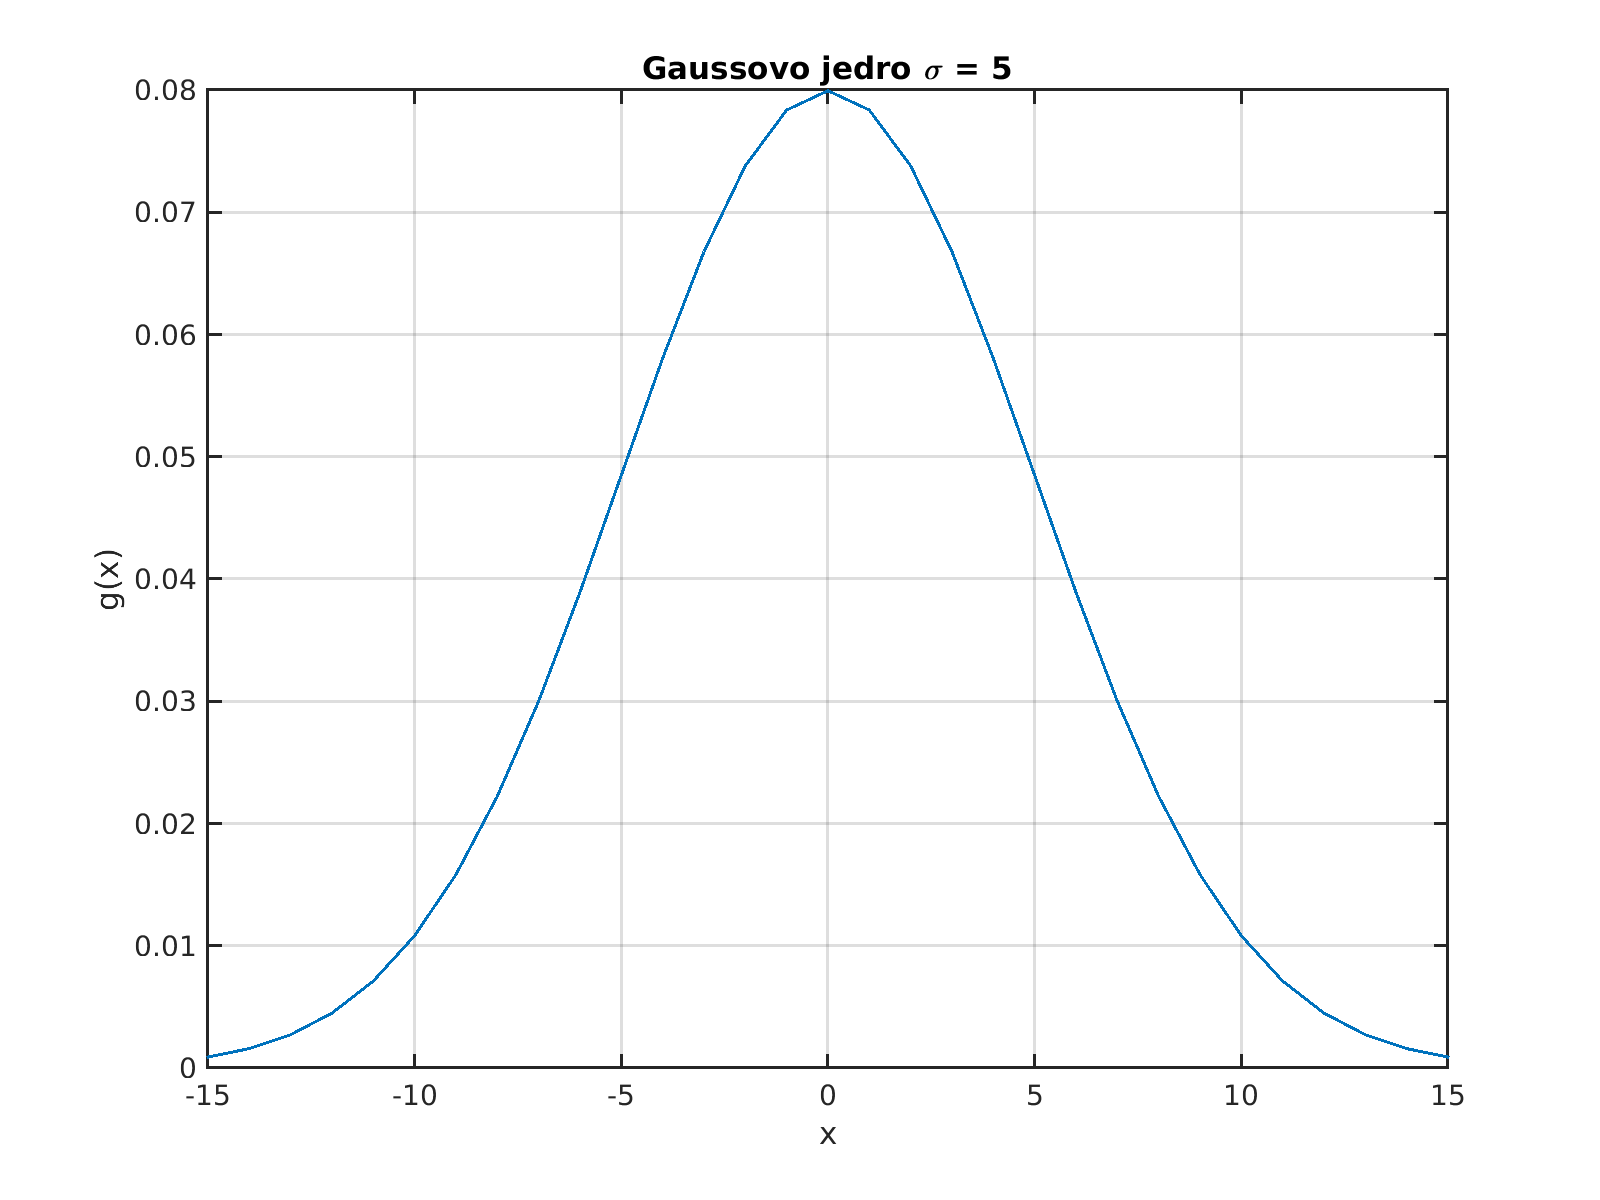
\includegraphics[width=0.7\columnwidth]{./Slike/gauss-kernel.png}
\caption{Gaussovo jedro s standardnim odklonom $\sigma=5$. }
\label{fig:gauss}
\end{figure}


Gaussov filter je vrsta filtra tekočega povprečja, ki je zelo primeren za izločevanje odvečnega šuma \cite{smith1997scientist}. Ker je karakteriziran z impulznim odzivom, ki je simetričen okoli ničelnega vzorca, gre za vrsto filtra z ničelno fazo. To pomeni, da je faza v frekvenčnem prostoru vedno $0$ \cite{smith1997scientist}. Ker imamo pri takih filtrih negativne indekse, ga težje uporabljamo. 

Ponavadi filtre uporabljamo v rekurzivni obliki, saj je računanje hitrejše. Impulzni odziv rekurzivnega filtra ni simetričen, zato ima nelinearno fazo \cite{smith1997scientist}. To pomankljivost lahko odpravimo z uporabo dvosmernega filtriranja.

Pri \textbf{dvosmernem filtriranju} najprej filtriramo iz leve proti desni in nato iz desne proti levi \cite{smith1997scientist}. Dobljena signala združimo in dobimo pravilen rezultat.







\section{Transformacija }
% Za testiranje optičnega toka in deskriptorjev, testiranje njihove robustnosti smo naredili več manipulacij, za boljšo predstavo o delovanju
\begin{equation}
\vec{M}_{int} = \begin{bmatrix}
	f_u & 0 & c_u \\
    0 & f_v & c_v \\
    0 & 0 & 1
\end{bmatrix}
\label{eq:intrinsic}
\end{equation}

\begin{equation}
\vec{R}_\phi = \begin{bmatrix}
\cos(\phi) & - \sin(\phi) & 0 \\
\sin(\phi) & \cos(\phi) & 0 \\
0 & 0 & 1
\end{bmatrix}
\label{eq:roll}
\end{equation}

\begin{equation}
\vec{R}_\theta = \begin{bmatrix}
1 & 0 & 0 \\
0 & \cos(\theta) & - \sin(\theta) \\
0 & \sin(\theta) & \cos(\theta)
\end{bmatrix}
\label{eq:pitch}
\end{equation}

\begin{equation}
\vec{R}_\psi = \begin{bmatrix}
\cos(\psi) & 0 & \sin(\psi) \\
0 & 1 & 0 \\
- \sin(\psi) & 0 & \cos(\psi) 
\end{bmatrix}
\label{eq:yaw}
\end{equation}


\begin{equation}
\vec{R} = \vec{R}_\phi \vec{R}_\theta \vec{R}_\psi
\label{eq:rotation}
\end{equation}


\begin{equation}
\vec{M}_{ext} = \begin{bmatrix}
	\vec{R} & \vdots & \vec{t}
\end{bmatrix}
\label{eq:extrinsic}
\end{equation}


\begin{equation}
\vec{H} = \vec{M}_{int} \vec{M}_{ext}
\label{eq:homography}
\end{equation}


\section{Evaluacijske metrike}
rmse snr mera prekrivanja področja, rae r 



\section{Materiali}
\subsection{Zlati standard}
\subsection{Senzorji v lab}
\subsection{Senzorji na terenu}
\subsection{Sinhornizacija časa}




\chapter{Eksperimenti in rezultati}\label{sec:eksperimenti}
V tem poglavju predstavljamo eksperimente, ki smo jih izvedli v različnih okoljih. Z njimi smo naslovili energijsko porabo, kot osrednji fiziološki parameter, srčni utrip in dihanje. 

Srčni utrip smo obravnavali kot posrednik (ang. Proxy) za energijsko porabo. Prav tako smo z eksperimenti srčnega utripa želeli preizkusiti teorijo iz poglavja \ref{sec:srcni-utrip} o srčnem utripu kot slabem posredniku.

Z eksperimenti detekcije dihanja smo želeli preizkusiti predlagano metodo za širšo uporabo.

Pri vseh naslovljenih fizioloških parametrih smo s pomočjo strojnega učenja izvajali predikcijo časovnih signalov $eem(t)$ za energijsko porabo, $hr(t)$ za srčni utrip in $dihanje(t)$ za dihanje. Predikcijo smo izvajali iz posamezne slike zaporedja video posnetka. Pri tem smo najprej generirali sliko optičnega ali prostorskega toka in nato določili področje, kjer se nahaja merjenec. Iz izbranega področja smo izračunali vektorje značilk $\vec{x}(t)$, te pa smo uporabili za predikcijo. Rezultat je zelo enostaven, realno-časoven model, ki ga lahko razširimo s temporalnim modeliranjem, če bi se pojavila potreba. Shema generalnega postopka je prikazana na sliki \ref{fig:shema-generalnega-postopka}.

\begin{figure}
\caption{}
\label{fig:shema-generalnega-postopka}
\end{figure}

Eksperimente smo kronološko razdelili na tri glavne dele: preliminarni testi, eksperimenti 1. faze in eksperimenti 2. faze. V \textbf{preliminarnih testih} opisujemo teste, s katerimi smo določili optimalne vrednosti parametrov, ki smo jih uporabili v metodah v nadaljevanju. 

Z \textbf{eksperimenti 1. faze} smo analizirali observabilnost izbranih fizioloških parametrov. Parameter je observabilen, če obstaja neničelna (pozitivna) korelacija med našo estimacijo iz značilk gibanja in merjenih vrednosti, ki smo jih dobili iz zanesljivih metod pridobivanja fizioloških parametrov. V 1. fazi smo posebej naslovili laboratorijske eksperimente tekalne steze, terenske eksperimente squash igre ter eksperimente dihanja.

V \textbf{eksperimentih 2. faze} smo optimizirali segmente generalnega postopka estimacije fizioloških parametrov. Sledi končna preiskava. Končna preiskava je sestavljena iz laboratorijske in terenske preiskave, kjer smo uporabili tri različne protokole.

V tem poglavju so na začetku opisane tudi implementacije nekaterih metod, opisanih v poglavju \ref{sec:metode}. Gre za tiste metode, kjer iz teoretične podlage implementacija ni bila točno razvidna. Opisane so tudi metode, ki nimajo teoretične podlage, saj gre samo za specifično implementacijo.

Na koncu sledijo še rezultati posameznih eksperimentov.







\section{Implementacija metod}
\subsection{Optični tok}
Na podlagi opisanih lastnosti metod optičnega toka v poglavju \ref{sec:metode-of} smo se odločili, da bomo v tem delu uporabili diferencialno metodo. Kljub višji računski zahtevnosti, ki ob današnji tehnologiji ne predstavlja več takega problema, smo želeli računati gost optični tok. Z gostim optičnim tokom tako dobimo natačno aproksimacijo polja gibanja za celotno telo. Prav tako nimamo problemov pri estimaciji energijske porabe za hitre gibe, kot bi bilo to v primeru uporabe ujemlanih metod. Ker je glavni namen uporaba in ne implementacija diferencialne metode, smo se osredotočili na Farneb{\"a}ck algoritem, ki je dostopen v knjižnici OpenCV.

\subsection{Prostorski tok}
Ker smo v našem delu za računanje prostorskega toka uporabili Kinect senzorje, smo potrebovali metodo, ki temelji na RGB-D podatkih. Ker je glavni namen uporaba in ne implementacija algoritma prostorskega toka, smo se osredotočili na PD-Flow algoritem, ki je javno dostopen \cite{jaimez2015primal}. Algoritem je podrobneje opisan v poglavju \ref{sec:pd-flow}.

\subsection{Sledilniki}
\subsubsection{Način izbire sledilnikov}\label{sec:pogoji-sledilnikov}
Pri izbiri sledilnikov smo se osredotočili na pogoje, ki jim morajo sledilniki v največji meri zadostiti.

\paragraph{Način sledenja.} Sledilnik mora dobro slediti osebam, ostali objekti niso pomembni. Sledenje mora biti zanesljivo, saj je od njega odvisna merilna napaka. Pri tem moramo upoštevati delovanje tudi v primerih, kadar tarča izgine iz slike. Sledenje mora delovati čimdaljši čas tako, da ne potrebujemo ponovne inicializacije. Inicializacijo sledilnika moramo opraviti samo na prvi sliki zaporedja, kar pomeni, da mora sledilnik vsebovati indirektno učenje (angl. offline training).

\paragraph{Implementacija.} Zaradi uporabe sledilnika v merilnem instrumentu, mora ta delovati v realnem času oziroma čim hitreje. Ker namen tega dela ni implementacija sledilnika, mora biti ta implementiran v prosto dostopni izvorni kodi. 


\subsubsection{Sledilnik za optični tok}
Na podlagi že prej opisanih pogojev, smo za merilno metodo z optičnim tokom našli sledilnik TLD avtorja Kalal et. al \cite{kalal2012tracking}. Prosto dostopne so tri implementacije sledilnika in sicer v knjižnici ccv (CCV-TLD), v knjižnici OpenCV (OPENCV-TLD) in c++ izvorna koda (NEBEHAY-TLD). Implementaciji iz knjižnic ccv in OpenCV se nekoliko razlikujeta od izvirnega dela \cite{kalal2012tracking}, NEBEHAY-TLD pa je samo prepis matlabove izvorne kode. 

Ker ni nobena implementacija zadovoljivo delovala na testnih squash posnetkih, smo poskusili še sledilnikom KCF \cite{danelljan2014adaptive} in CORR \cite{danelljan2014accurate}. KCF je implementiran v knjižnici OpenCV, CORR pa v knjižnici Dlib \cite{king2009dlib}.

Testiranje sledilnikov je opisano v poglavju \ref{sec:testiranje-sledilnikov-za-opticni-tok}, kjer smo ugotovili, da najbolje deluje sledilnik KCF. Tega smo tudi uporabili v naših nadaljnih eksperimentih.

\subsubsection{Sledilnik za prostorski tok}
Na podlagi pogojev iz poglavja \ref{sec:pogoji-sledilnikov} smo za merilno metodo s prostorskim tokom našli le DS-KCF sledilnik avtorja Hannuna et. al \cite{hannuna2016ds}. 

\subsection{Kalmanov filter}
Za prostor stanj smo izbrali stanje hitrosti $v$ in pospeška $a$ \eqref{eq:stanje}. 

\begin{equation}
\vec{x}(k) = \begin{bmatrix}
					v(k) & a(k)
				\end{bmatrix}^\top 
                \label{eq:stanje}
\end{equation}

Matrika prehajanja stanj je določena z enačbo \eqref{eq:a}.

\begin{equation}
\vec{A} = \begin{bmatrix}
				1 & 1 \\
                0 & 1
			\end{bmatrix} 
            \label{eq:a}
\end{equation}

Za matriko vhodnih stanj $G$ smo izbrali \eqref{eq:g}, s katero modeliramo neznane vhodne parametre hitrosti $v_n$ in pospeška $a_n$ v vektorju $u$ \eqref{eq:u}. 

\begin{equation}
\vec{G} = \begin{bmatrix}
				1 & 0
			\end{bmatrix}^\top 
            \label{eq:g}
\end{equation}

\begin{equation}
\vec{u}(k) = \begin{bmatrix}
					v_{n}(k) & a_n(k)
				\end{bmatrix}^\top 
                \label{eq:u}
\end{equation}


Merilna matrika je predstavljena z enačbo \eqref{eq:h}
\begin{equation}
\vec{H} = \begin{bmatrix}
				1 & 0
			\end{bmatrix}^\top 
            \label{eq:h}
\end{equation}

Za začetno hitrost in pospešek smo izbrali vrednost $0$, ker se naši testi večinoma začnejo v mirovanju. 

Variance šuma modela gibanja, merilnega modela in konvaričane matrike stanja smo določili z uporabo mrežnega iskanja, ki je opisan v poglavju \ref{sec:optimizacija-svm-parametrov}. Pri tem smo uporabili labele učnih vzorcev vseh testov 1. sklopa eksperimentov za referenco, njihove pošumljene ocene pa za meritev. Varianca šuma merilnega modela je tako znašala $\sigma_\vec{z}^2 = 0.04$, varianca šuma modela gibanja pa $\sigma_\vec{x}^2 = 456.13$. Za kovariančno matriko predikcije smo uporabili varianco $\sigma_\vec{P}^2 = 456.13$. Kovariančno matriko modela gibanja smo določili po enačbi \eqref{eq:Q}, kovariančna matrika merilnega modela je bila določena z enačbo \eqref{eq:R} in začetna vrednost kovariančne matrike stanja z \eqref{eq:P}.

\begin{equation}
\vec{Q} = \vec{G} \vec{G}^\top \sigma_\vec{x}^2
\label{eq:Q}
\end{equation}

\begin{equation}
\vec{R} = \sigma_\vec{z}^2
\label{eq:R}
\end{equation}

\begin{equation}
\vec{P}(0) = \begin{bmatrix}
1 & 0 \\
0 & 1
\end{bmatrix} \sigma_\vec{P}^2
\label{eq:P}
\end{equation}










\subsubsection{Implementacija Gaussovega filtra}
Gaussovo jedro smo implementirali po enačbi \eqref{eq:gauss} in ga nato še normirali. Za filtriranje podatkov smo uporabili Matlabovo funkcijo \texttt{filtfilt}, ki je primerna za hitro računanje s filtri z ničelno fazo, saj uporablja tehniko dvosmernega filtriranja.


\subsection{Projektivna transformacija preliminarnih testov}
Projektivno transformacijo smo izvedli s pomočjo matlabovih funkcij \texttt{fitgeotrans} in \texttt{imwarp}. Za vhodne točke smo izbrali robove posamezne slike zaporedja. Za izhodne točke smo izbrali vrednosti v tabeli \ref{tab:projective}, pri čemer so $h$ dolžina slike $w$ širina slike ter $x$ in $y$ slikovni koordinati.

\begin{table}[htb]
\centering
\begin{tabular}{l S[table-format=1.3] S[table-format=1.3] }
	\toprule
	\thead{Točka} & \thead{$\mathbf{x~[\times w]}$} & \thead{$\mathbf{y~[\times h]}$} \\
    \midrule
	$P_0$ & 0 & 0.25 \\
    $P_1$ & 1 & 0 \\
    $P_2$ & 0.125 & 0.75 \\
    $P_3$ & 0.875 & 0.875 \\
    \bottomrule
\end{tabular}
\caption{}
\label{tab:projective}
\end{table}

\subsection{Simulacija vibracij kamere}
Kadar uporabljamo ročne kamere, pogosto pride do tresenja. Vibracije smo simulirali z majhnimi naključnimi premiki in rotacijo posameznih slik iz video zaporedja. Vsako sliko smo transformirali z Evklidsko transformacijo. Pri tem smo translacijo omejili na \SI{4}{\%} velikosti slike. Rotacija je bila omejena na \SI{0.13}{rad}. 

Translacijo in rotacijo smo filtrirali še s Kalmanovim filtrom, tako da smo dobili bolj realistično simulacijo. Za Kalmanov filter smo uporabili enak model, kot je predstavljen v poglavju \ref{sec:kalmanov-filter}. Začetne variance filtra smo določili empirično tako, da smo dobili čimbolj realistične rezultate. Varianca šuma merilnega modela je znašala $\sigma_\vec{z}^2=1024$, variancal šuma modela gibanja pa $\sigma_\vec{x}^2=2$. Za kovariančno matriko predikcije smo uporabili varianco $\sigma_\vec{P}^2=2$.


\subsection{Združevanje slik iz dveh Kinect kamer}
Zaradi ozkega vidnega polja Kinect kamer smo za pokritje celotne širine igrišča potrebovali dve kameri. Zaporedja slik smo pred nadaljno obdelavo morali združiti v eno zaporedje glede na opazovanega igralca.

Zajem iz posameznih kamer ni bil sinhroniziran, zato smo pred združevanjem sinhronizirali posnetka tako, da smo izbrali slike iz posameznega zaporedja z najbolj podobnimi časovnimi žigi.

Časovno sinhornizirana zaporedja slik smo nato poskušali združiti s tremi različnimi metodami:  združevanje z značilkami, združevanje s kontrolnimi točkami in prilagojeno združevanje. Testiranja teh metod so opisana v poglavju \ref{sec:zdruzevanje}. Kot najbolj usešno metodo smo nato uporabili \textbf{prilagojeno združevanje}.



\section{Preliminarni testi}
\subsection{Deskriptorji}
\subsubsection{Optimizacija HOOF deskriptorjev}
Parameter $N_{HOOF}$ smo določili na podlagi rezultatov evaluacije v tabeli \ref{tab:nhoof} in grafov korelacije med referenčnimi podatki in predikcijo \ref{fig:corr-hoof}. Za evaluacijo smo uporabili učne vzorce hrbtne kamere preliminarnih laboratorijskih testov. Evaluirali smo samo za podatke energijske porabe $W$. Pridobljene značilke deskriptorjev smo normirali na intervalu $[-1,1]$ in jih uporabili za učenje regresijskega modela z metodo podpornih vektorjev $\epsilon$-SVR in jedrom RBF. Metode so podrobneje predstavljene v poglavju \ref{sec:matematicni-modeli}. Za določitev optimalnih parametrov, ki so predstavljeni v tabeli \ref{tab:nhoof-param}, smo uporabili optimizacijsko metodo mrežnega iskanja \cite{hsu2003practical}. Rezultate smo filtrirali še s Kalmanovim filtrom, ki je predstavljen v \ref{sec:kalmanov-filter}.

\begin{table}[htb]
	\centering
    \begin{tabular}{S[table-format=2.0] S[table-format=2.3] S[table-format=1.3] S[table-format=1.3] S[table-format=1.3]}
    \toprule
    \thead{$\mathbf{N_{HOOF}}$} & \thead{$\mathbf{C}$} & \thead{$\mathbf{\gamma}$} & \thead{$\mathbf{\epsilon}$} & \thead{MSE} \\ 
    \midrule
    30 & 8 & 0.707 & 0.812 & 7.903 \\
    60 & 8 & 0.354 & 0.379 & 7.320 \\
    120 & 11.314 & 0.177 & 0.536 & 6.998 \\
    160 & 11.314 & 0.125 & 0.616 & 6.832 \\
    \bottomrule
    \end{tabular}
    \caption[Optimalni parameteri RBF jedra modelov za določitev $N_{HOOF}$]{Optimalni parametri RBF jedra za modele z različnim številom stolpcev $N_{HOOF}$ v HOOF deskriptorju.}
    \label{tab:nhoof-param}
\end{table}

V tabeli \ref{tab:nhoof} lahko vidimo, da se povečevanjem števila stolpcev rezultati bistveno ne razlikujejo. Najbojlši rezultate nam sicer daje $120$ stolpcev, vendar pa smo za potrebe naše metode uporabili $N_{HOOF}=60$, ki je ravno tako dal zadovoljive rezultate. S takim številom smo zagotovili dobro delovanje glede na minimalno vrednost, še vseeno pa ne gre za tako veliko število, ko bi do izraza prišle amplitude šumnih vektorjev.

\begin{table}[htb]
	\centering
    \begin{tabular}{S[table-format=2.0] S[table-format=1.3] S[table-format=1.3] S[table-format=1.3] S[table-format=2.2]}
    \toprule
    \thead{$\mathbf{N_{HOOF}}$} & \thead{$\mathbf{r}$} & \thead{RAE} & \thead{RRSE} & \thead{nSV [\%]}\\
    \midrule%nSV
    30 & 0.978 & 0.296 & 0.304 & \boldentry{2.2}{62.81}\\%18089
    \boldentry{2.0}{60} & 0.980 & 0.277 & 0.289 & 81.21\\%23388
    120 & \boldentry{1.3}{0.983} & \boldentry{1.3}{0.261} & \boldentry{1.3}{0.273} & 74.39\\%21424
    160 & 0.982 & 0.272 & 0.284 & 71.68\\%20644
    \bottomrule
    \end{tabular}
    \caption[Rezultati evaluacije modelov z različnim $N_{HOOF}$]{Rezultati evaluacije modelov z različnim številom stolpcev $N_{HOOF}$ HOOF deskriptorja. Optimalni rezultati so odebeljeni. Kljub dobrim rezultatom modela z $N_{HOOF}=120$ smo izbrali $N_{HOOF}=60$, ker nanj šum manj vpliva.}
    \label{tab:nhoof}
\end{table}

\begin{figure}[htb]
	\centering
    \begin{subfigure}[t]{0.45\columnwidth}
    	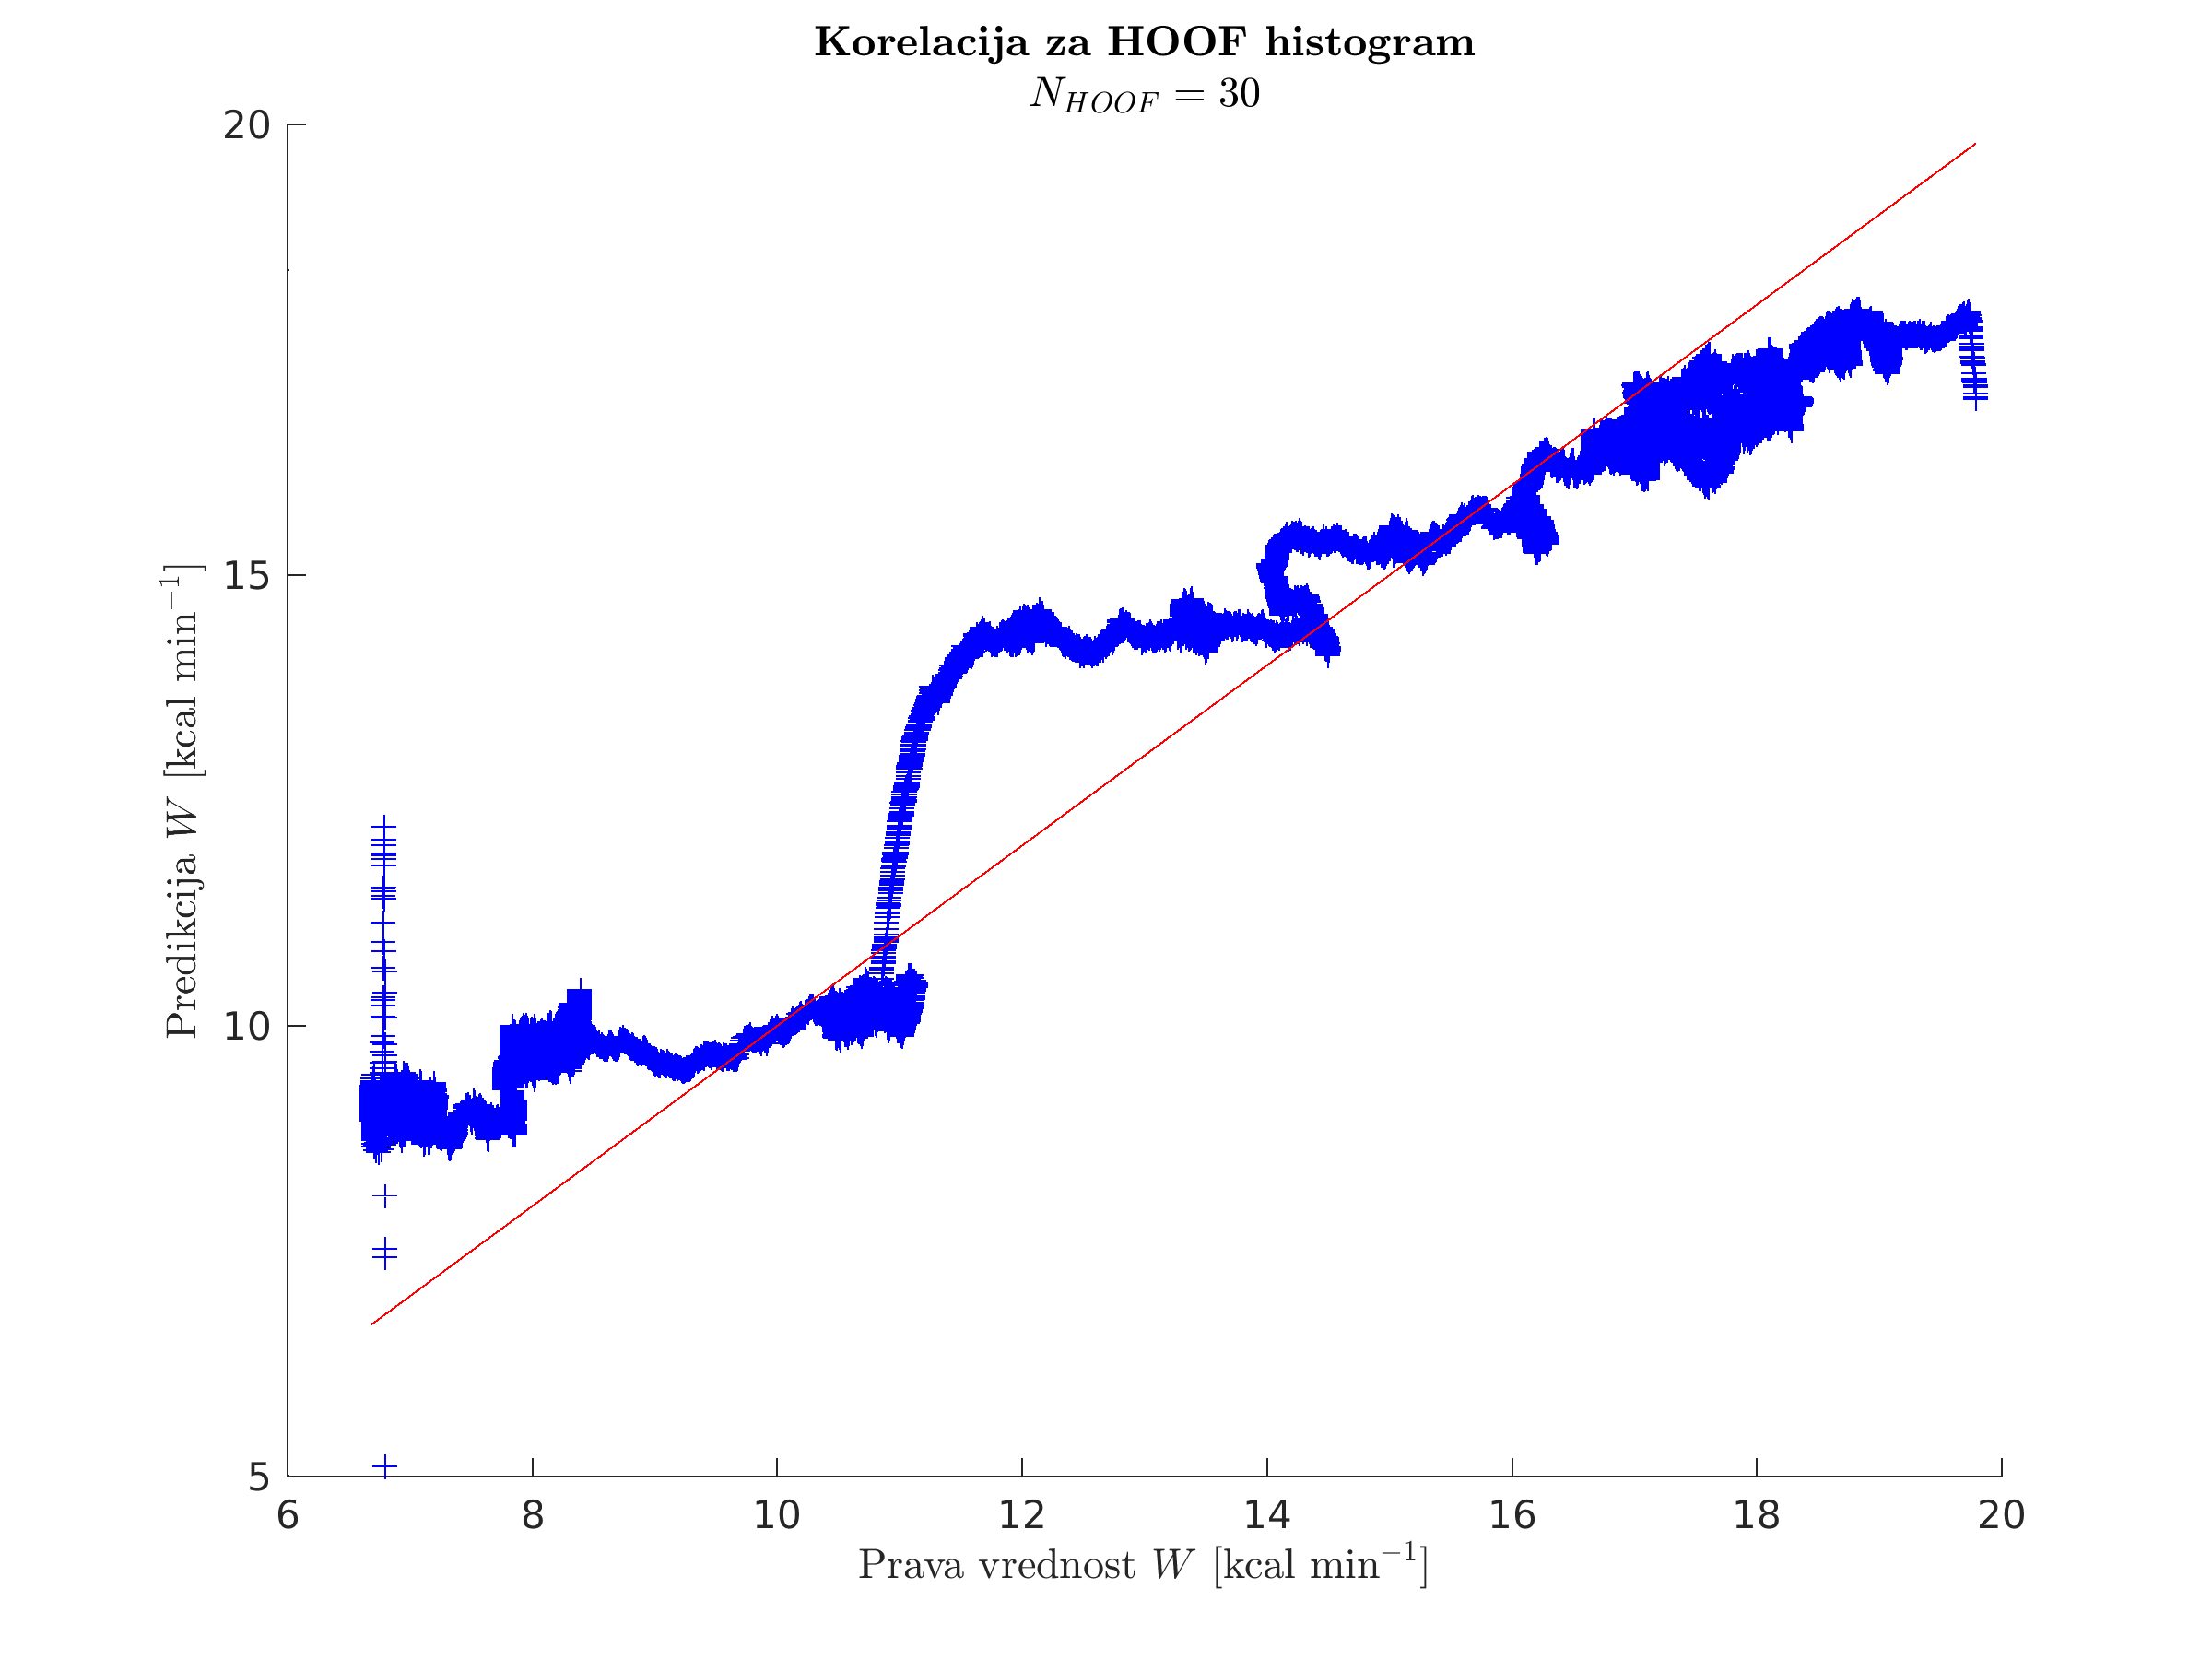
\includegraphics[width=\columnwidth]{./Slike/corr-hoof-30.png}
        \caption{Korelacija $N_{HOOF}=30$.}
        \label{fig:corr-hoof-30}
    \end{subfigure}
    ~
    \begin{subfigure}[t]{0.45\columnwidth}
      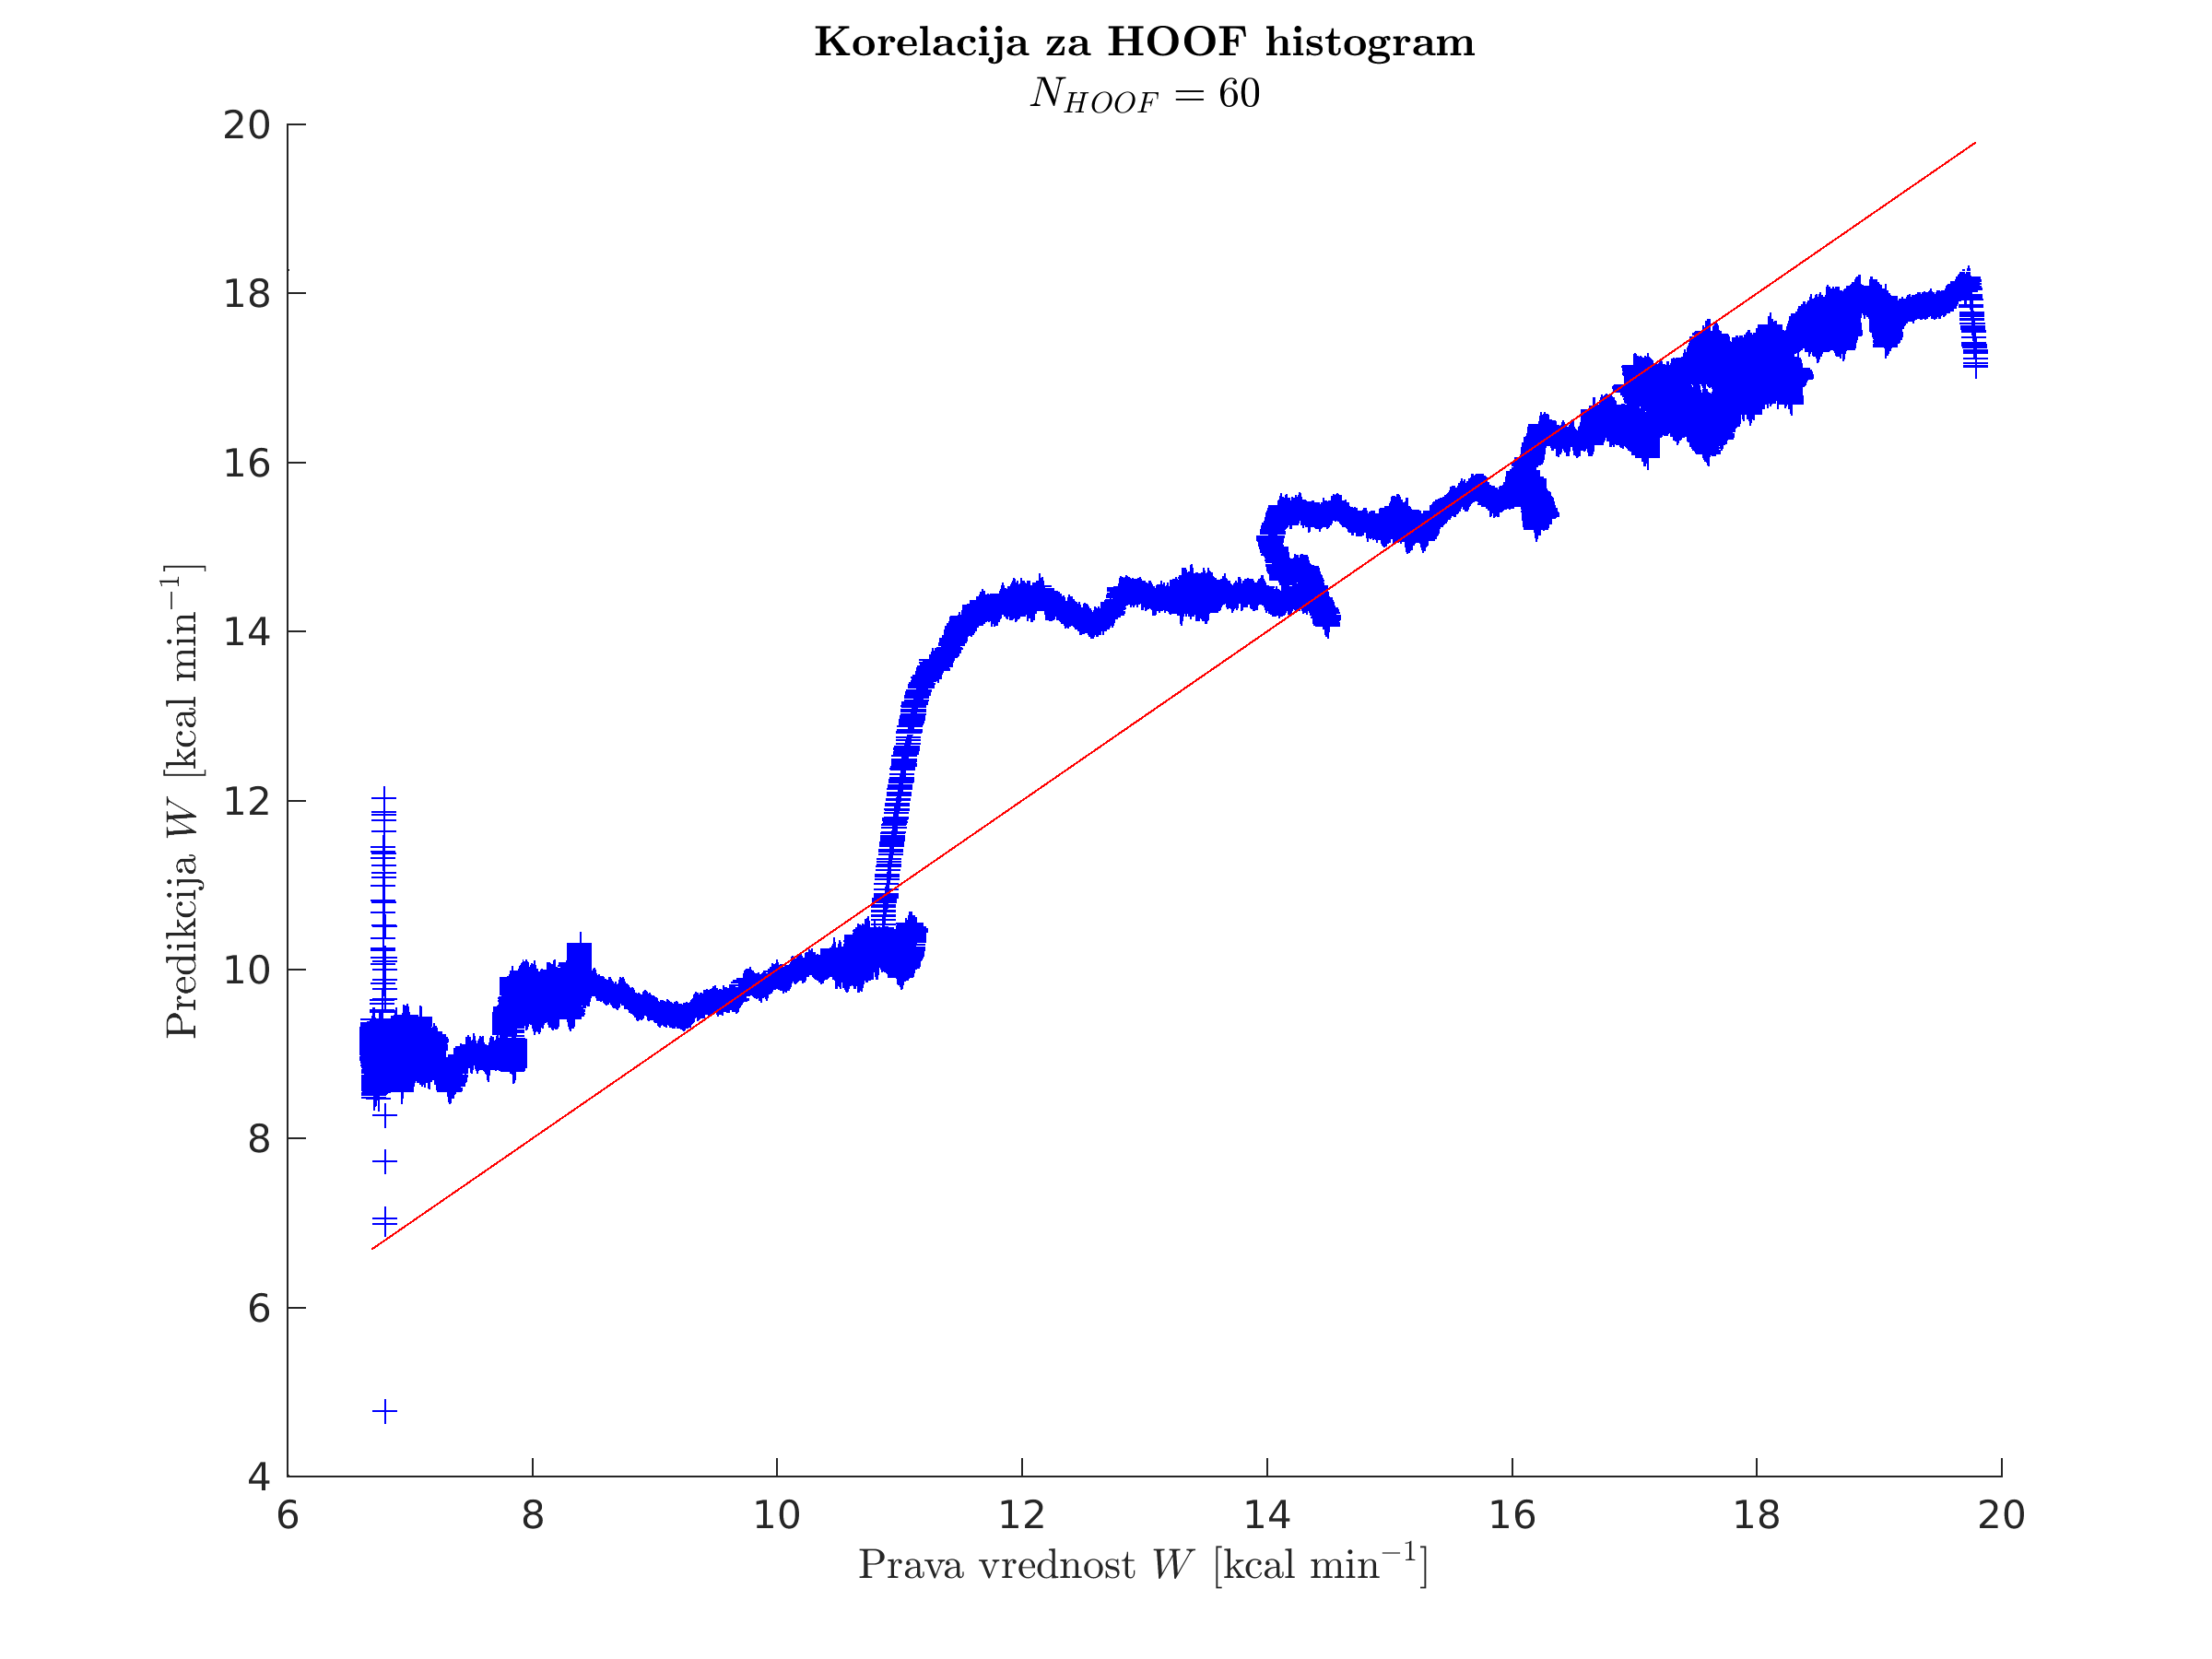
\includegraphics[width=\columnwidth]{./Slike/corr-hoof-60.png}
      \caption{Korelacija $N_{HOOF}=60$.}
      \label{fig:corr-hoof-60}
    \end{subfigure}
    ~
    \begin{subfigure}[b]{0.45\columnwidth}
      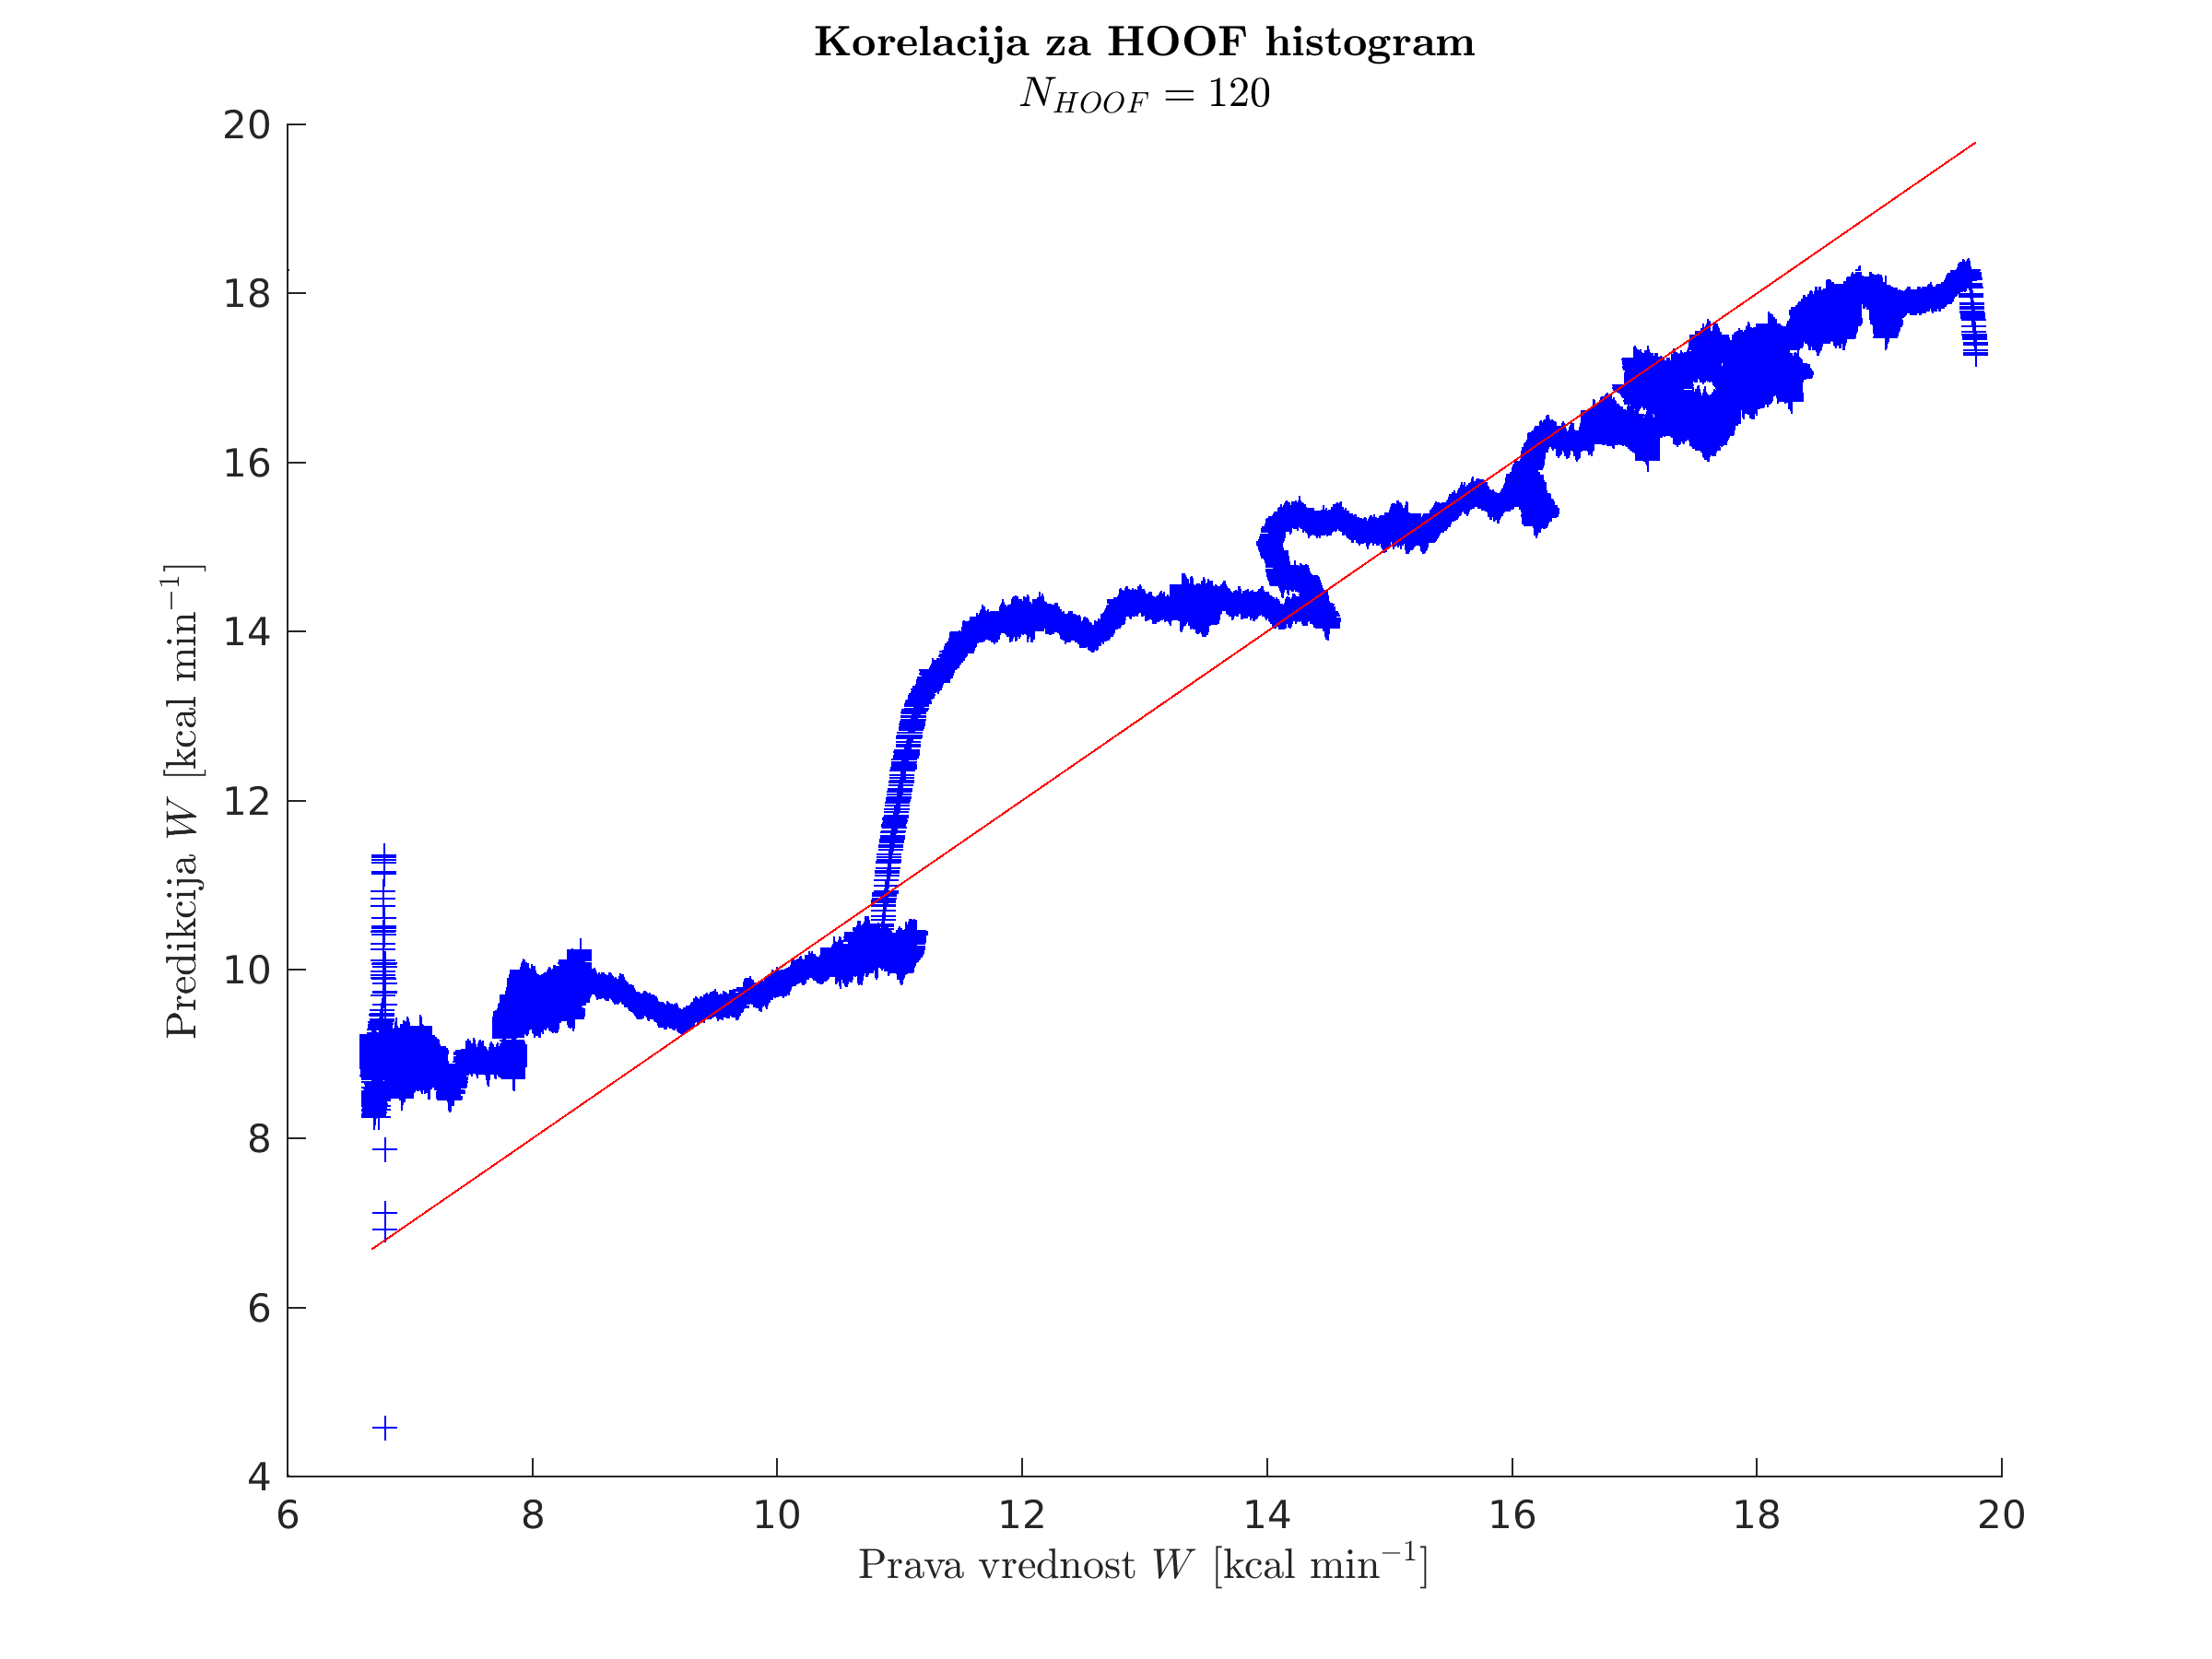
\includegraphics[width=\columnwidth]{./Slike/corr-hoof-120.png}
      \caption{Korelacija $N_{HOOF}=120$.}
      \label{fig:corr-hoof-120}
    \end{subfigure}
    ~
    \begin{subfigure}[b]{0.45\columnwidth}
      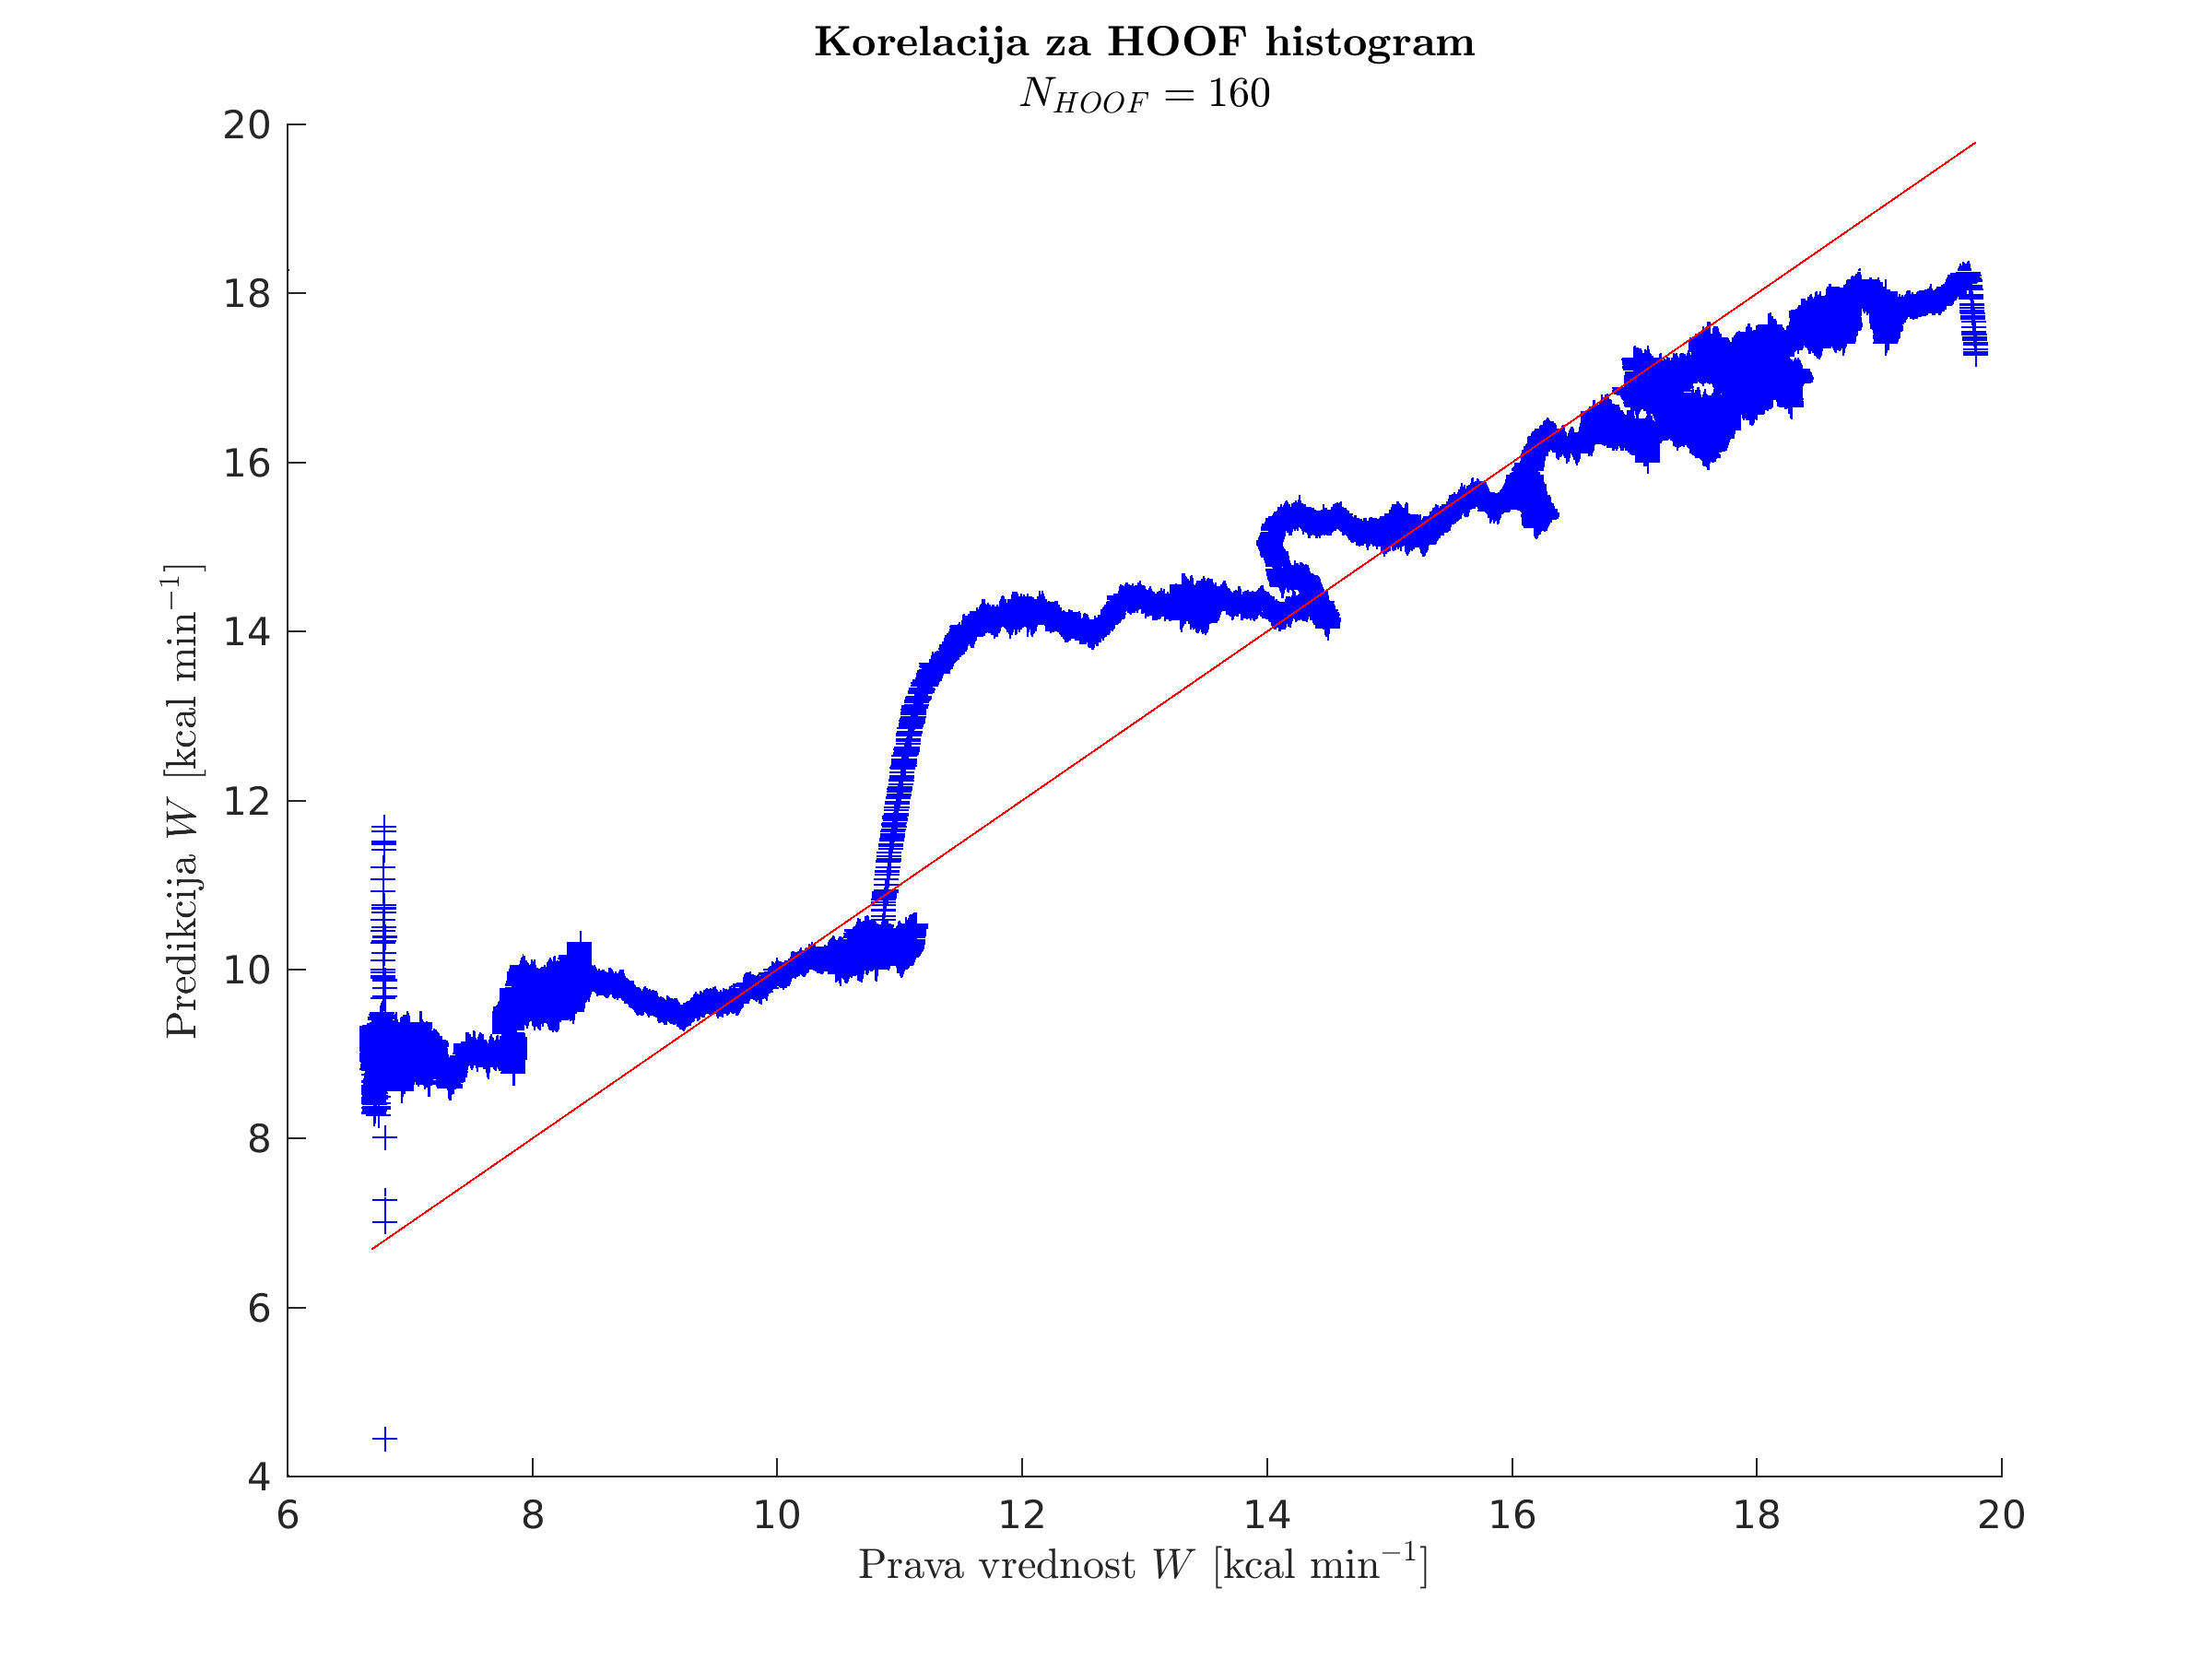
\includegraphics[width=\columnwidth]{./Slike/corr-hoof-160.png}
      \caption{Korelacija $N_{HOOF}=160$.}
      \label{fig:corr-hoof-160}
    \end{subfigure}
    \caption[Grafi korelacij modelov z različnim $N_{HOOF}$]{Grafi korelacij modelov z različnim številom stolpcev $N_{HOOF}$ HOOF deskriptorja. Rezultati so si zelo podobni.}
    \label{fig:corr-hoof}
\end{figure}





\subsubsection{Optimizacija HAFA deskriptorjev}
Parameter $N_{HAFA}$ smo določili na podlagi rezultatov evaluacije v tabeli \ref{tab:nhafa} in grafov korelacije med referenčnimi podatki in predikcijo \ref{fig:corr-hafa}. Za evaluacijo smo uporabili enak eksperimentalni protokol kot za HOOF značilke v poglavju \ref{sec:hoof}, s to razliko, da smo značilke normirali na intervalu $[0, 1]$ in odstranili stolpec z amplitudami $0.5$. S tem smo odstranili šum, ki se je pojavil, ko ni bilo nobenega gibanja. Amplitudo šuma smo določili, kot maksimalno vrednost amplitude, ki še ni predstavljala gibanja. Optimalni parametri evaluacijske metode so predstavljeni v tabeli \ref{tab:nhafa-param}.


\begin{table}[htb]
	\centering
    \begin{tabular}{S[table-format=2.0] S[table-format=2.3] S[table-format=1.3]  S[table-format=1.3] S[table-format=1.3]}
    \toprule
    \thead{$\mathbf{N_{HAFA}}$} & \thead{$\mathbf{C}$} & \thead{$\mathbf{\gamma}$} & \thead{$\mathbf{\epsilon}$} & \thead{MSE} \\ 
    \midrule
    30 & 8 & 5.657 & 0.616 & 4.329 \\
    60 & 8 & 5.657 & 0.616 & 4.327 \\
    120 & 8 & 5.657 & 0.616 & 4.327 \\
    160 & 8 & 5.657 & 0.616 & 4.327 \\
    \bottomrule
    \end{tabular}
    \caption[Optimalni parameteri RBF jedra modelov za določitev $N_{HAFA}$]{Optimalni parametri RBF jedra za modele z različnim številom stolpcev $N_{HAFA}$ v HAFA deskriptorju.}
    \label{tab:nhafa-param}
\end{table}

V tabeli \ref{tab:nhafa} lahko vidimo, da so rezultati praktično enaki. Za našo metodo smo izbrali $N_{HAFA}=60$, kar v grobem predstavlja $60$ različnih hitrosti z maksimalno amplitudo \SI{60}{px.f^{-1}}.

\begin{table}[htb]
	\centering
    \begin{tabular}{S[table-format=2.0] S[table-format=1.3] S[table-format=1.3] S[table-format=1.3] S[table-format=2.2]}
    \toprule
    \thead{$\mathbf{N_{HAFA}}$} & \thead{$\mathbf{r}$} & \thead{RAE} & \thead{RRSE} & \thead{nSV [\%]}\\
    \midrule%nSV
    30 & 0.984 & 0.213 & 0.231 & 62.08 \\%17879/28799
    \boldentry{2.0}{60} & \boldentry{1.3}{0.984} & \boldentry{1.3}{0.211} & \boldentry{1.3}{0.228} & \boldentry{2.2}{62.60} \\%18028
    120 & 0.984 & 0.211 & 0.228 & 62.63 \\%18037
    160 & 0.984 & 0.211 & 0.228 & 62.63 \\%18037
    \bottomrule
    \end{tabular}
    \caption[Rezultati evaluacije modelov z različnim $N_{HAFA}$]{Rezultati evaluacije modelov z različnim številom stolpcev $N_{HAFA}$ HAFA deskriptorja. Optimalni rezultati so odebeljeni.}
    \label{tab:nhafa}
\end{table}

\begin{figure}[htb]
	\centering
    \begin{subfigure}[t]{0.45\columnwidth}
    	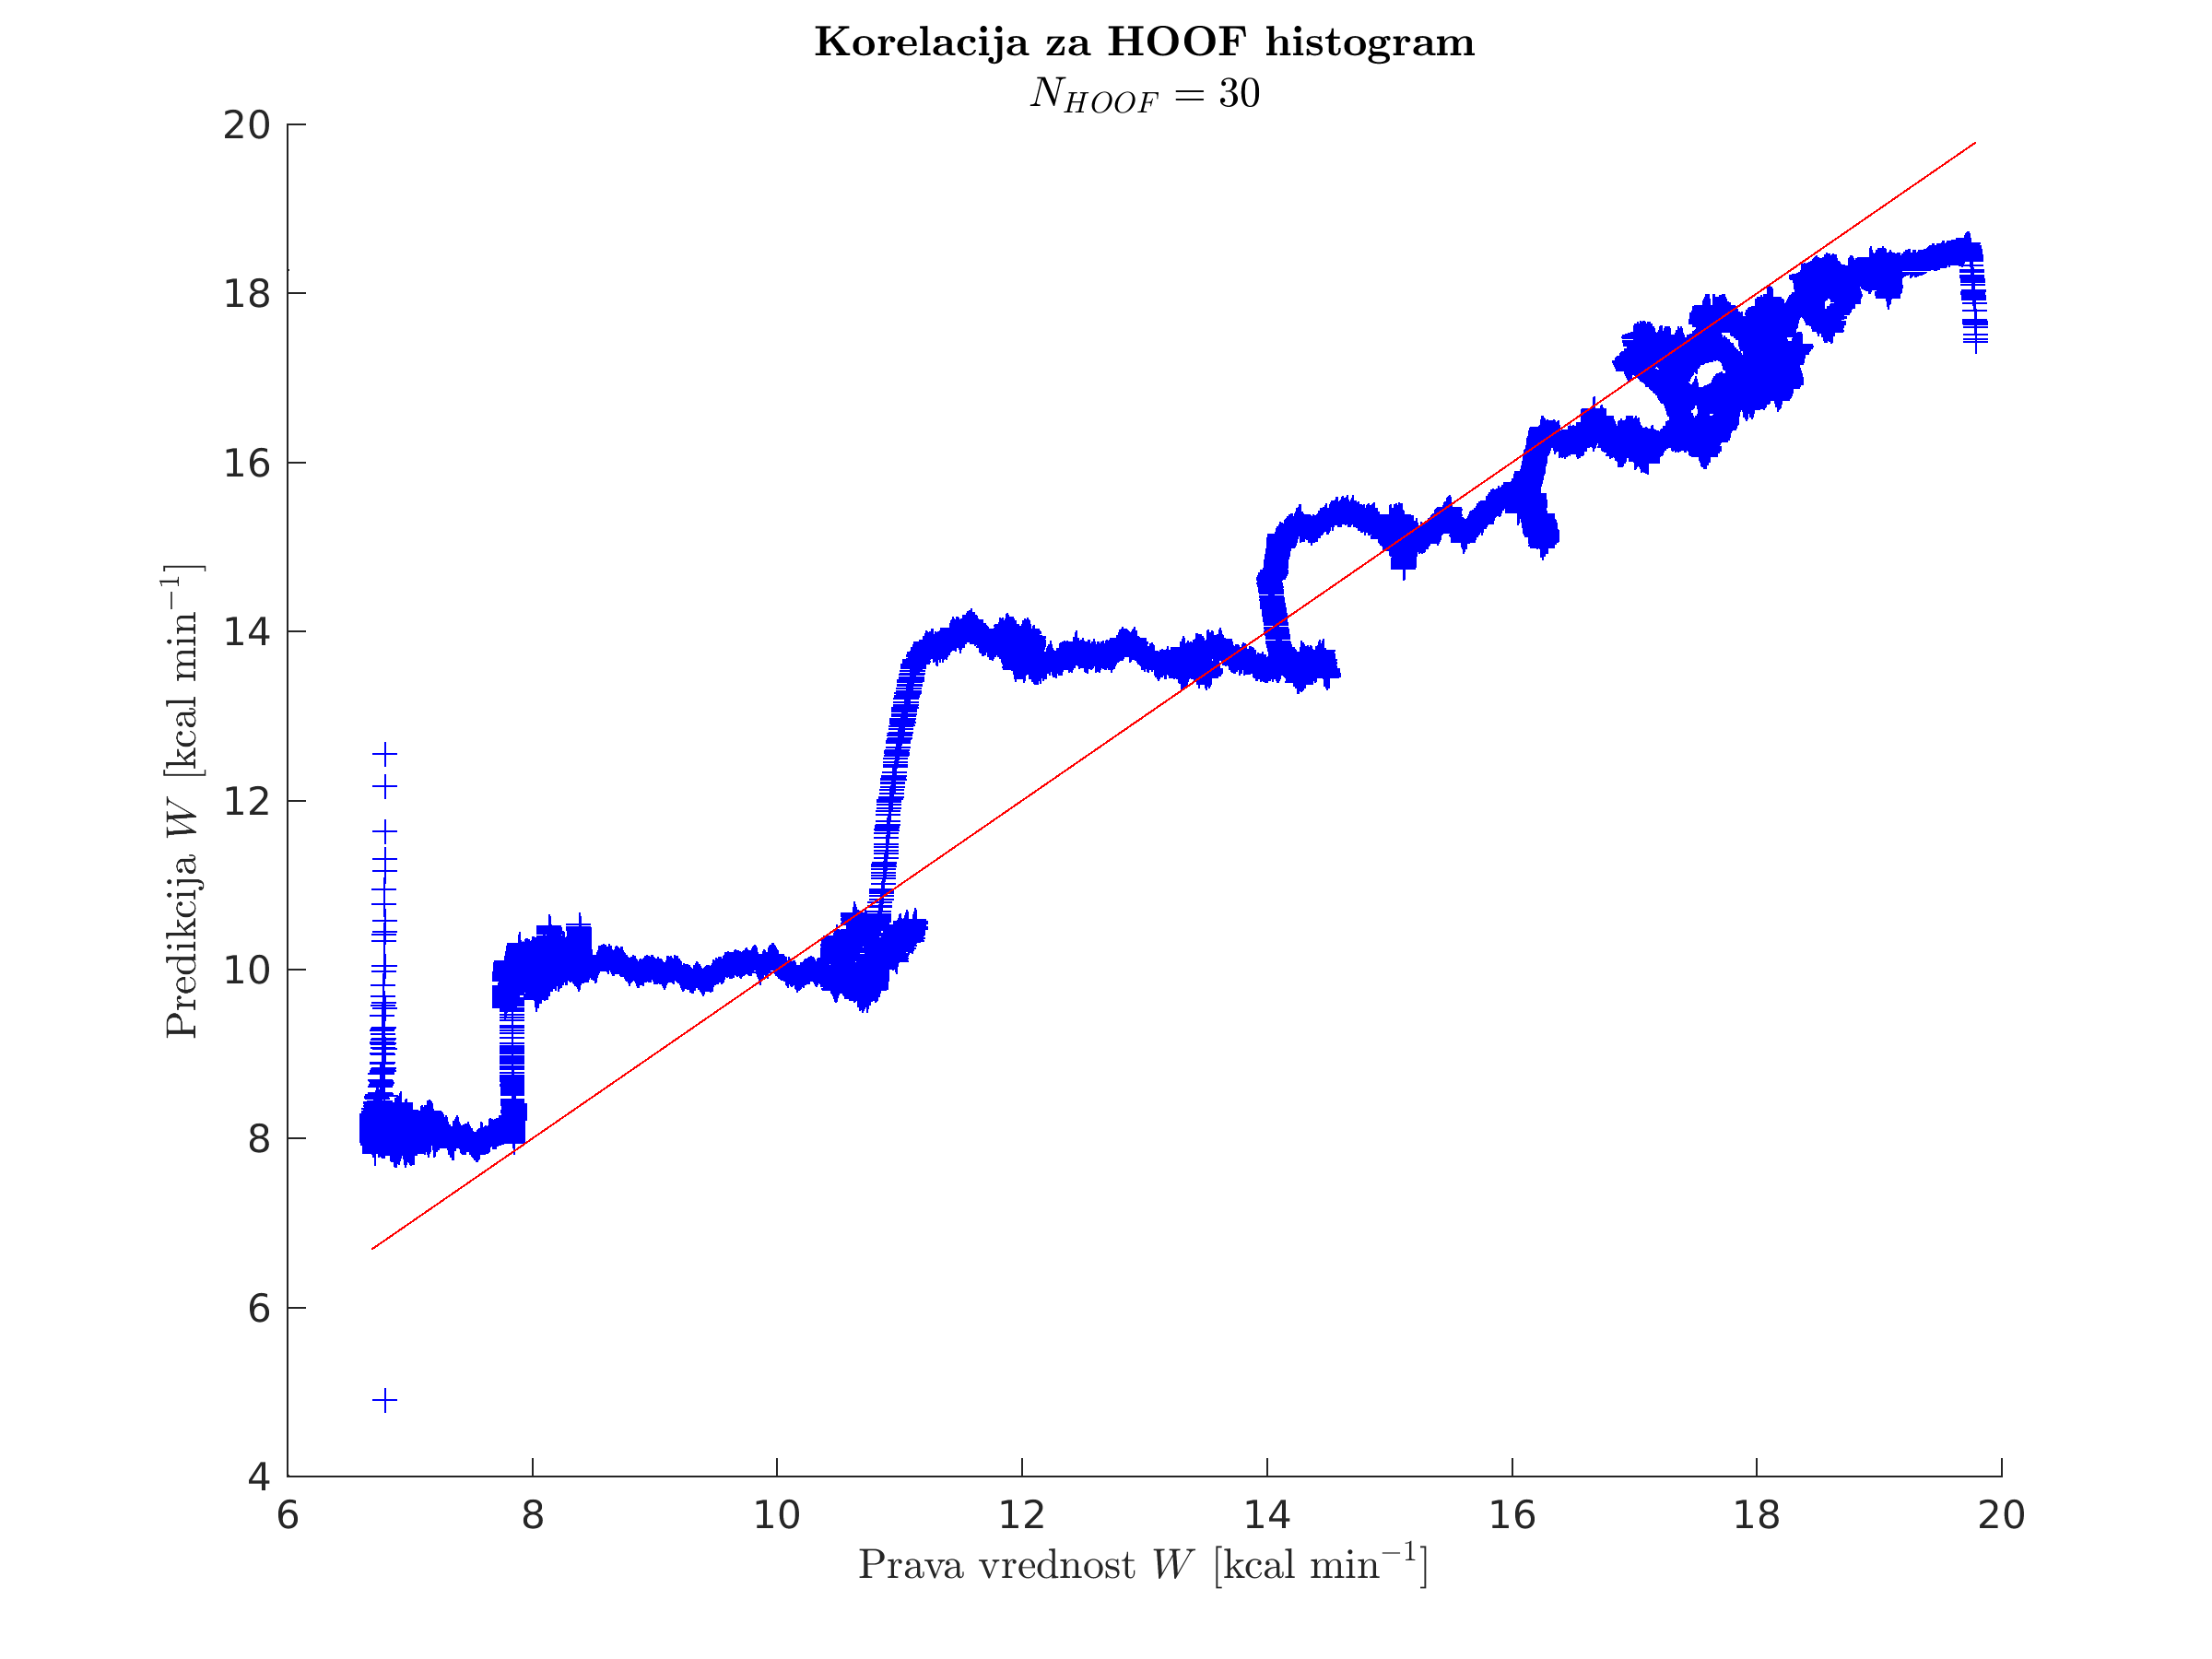
\includegraphics[width=\columnwidth]{./Slike/corr-hafa-30.png}
        \caption{Korelacija $N_{HAFA}=30$.}
        \label{fig:corr-hafa-30}
    \end{subfigure}
    ~
    \begin{subfigure}[t]{0.45\columnwidth}
      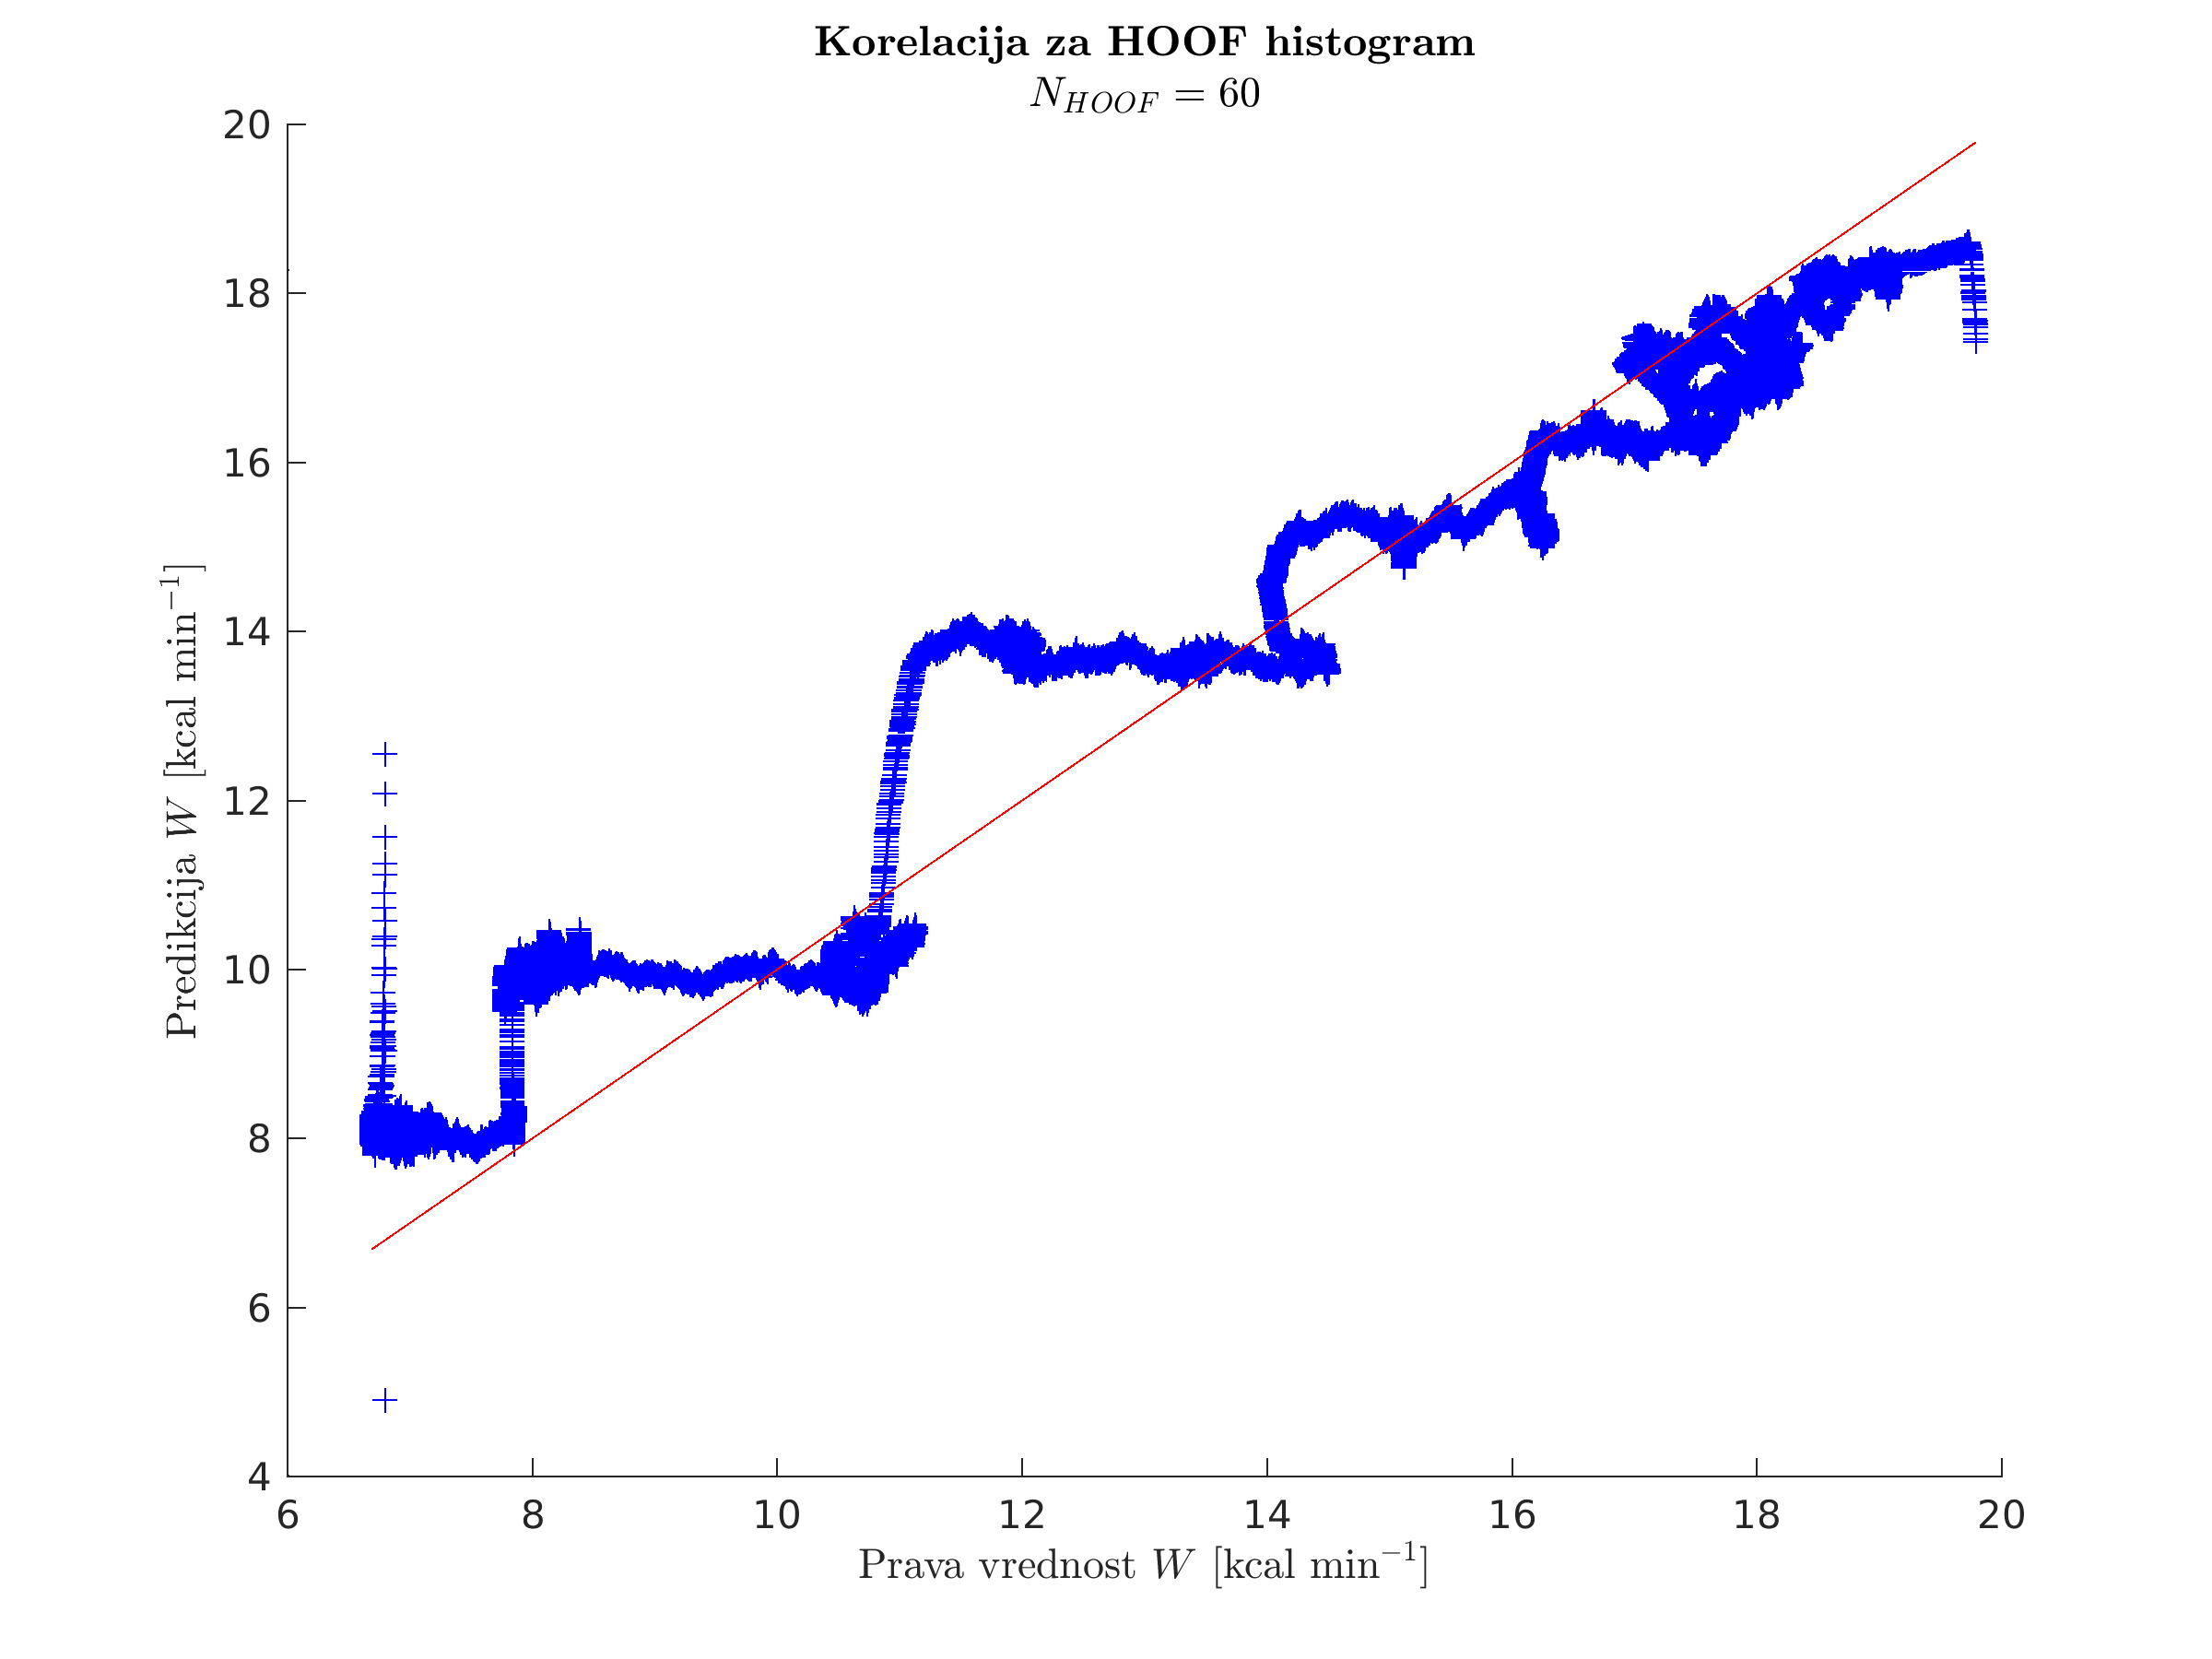
\includegraphics[width=\columnwidth]{./Slike/corr-hafa-60.png}
      \caption{Korelacija $N_{HAFA}=60$.}
      \label{fig:corr-hafa-60}
    \end{subfigure}
    ~
    \begin{subfigure}[b]{0.45\columnwidth}
      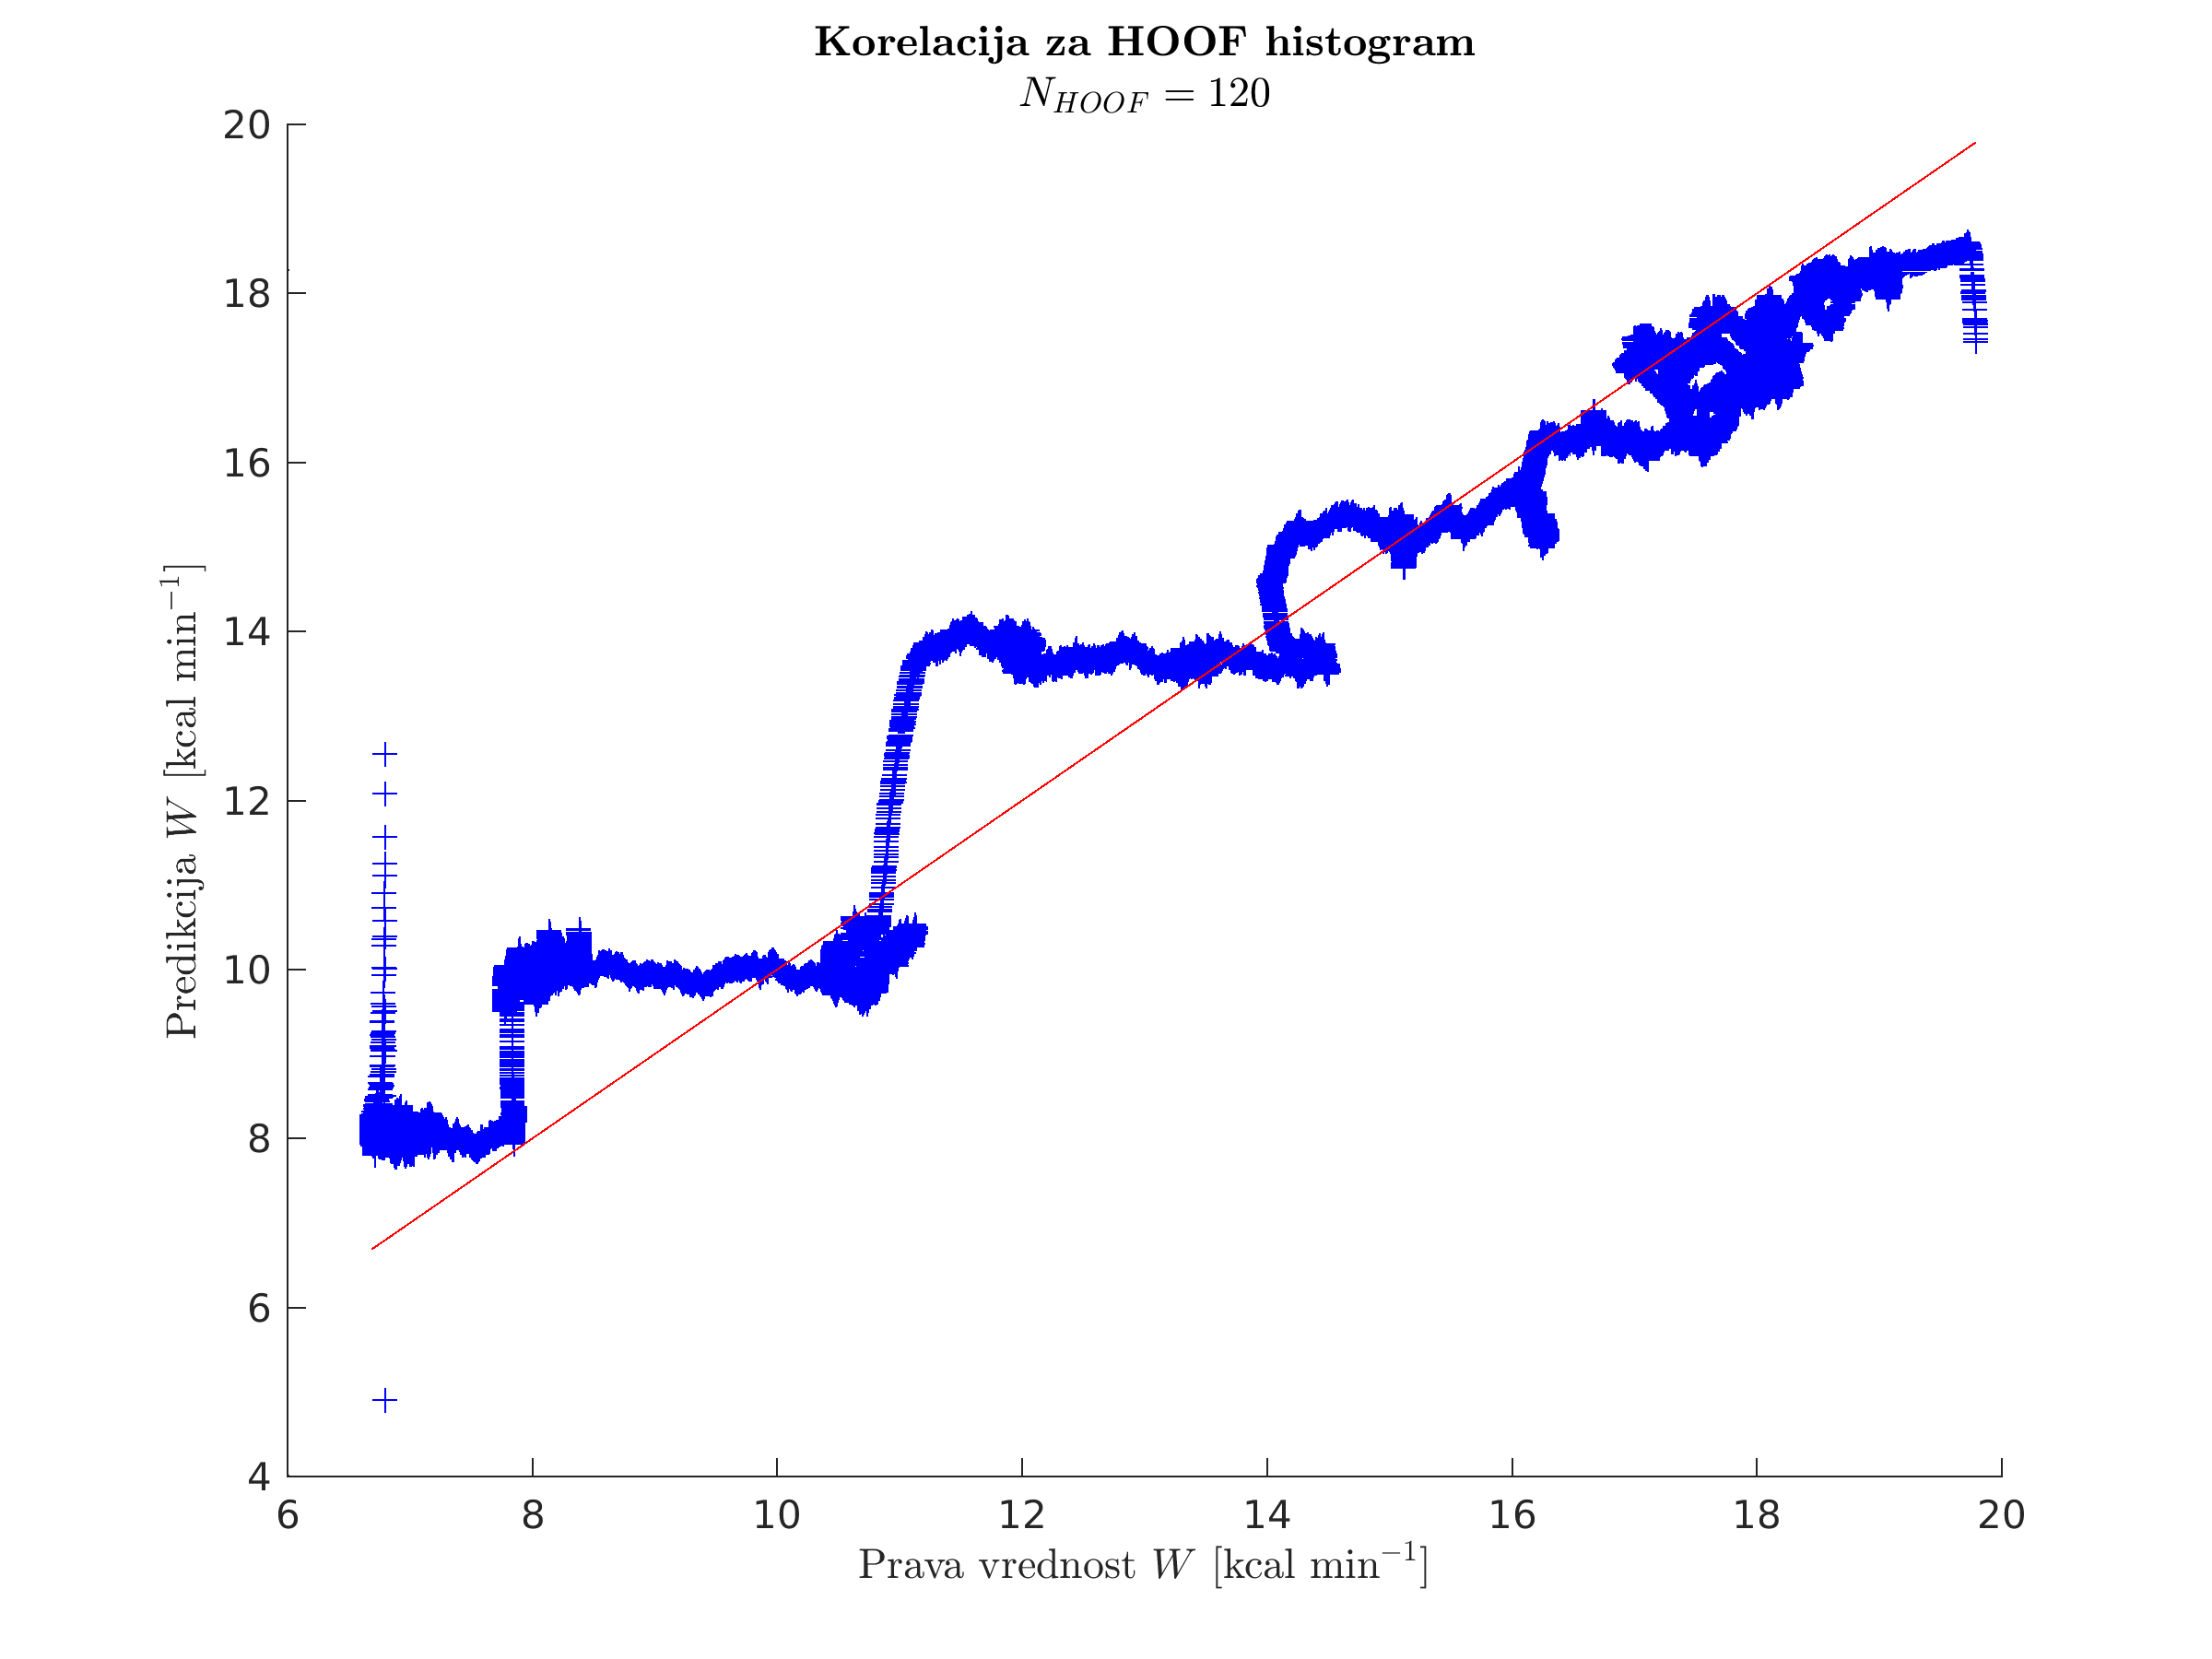
\includegraphics[width=\columnwidth]{./Slike/corr-hafa-120.png}
      \caption{Korelacija $N_{HAFA}=120$.}
      \label{fig:corr-hafa-120}
    \end{subfigure}
    ~
    \begin{subfigure}[b]{0.45\columnwidth}
      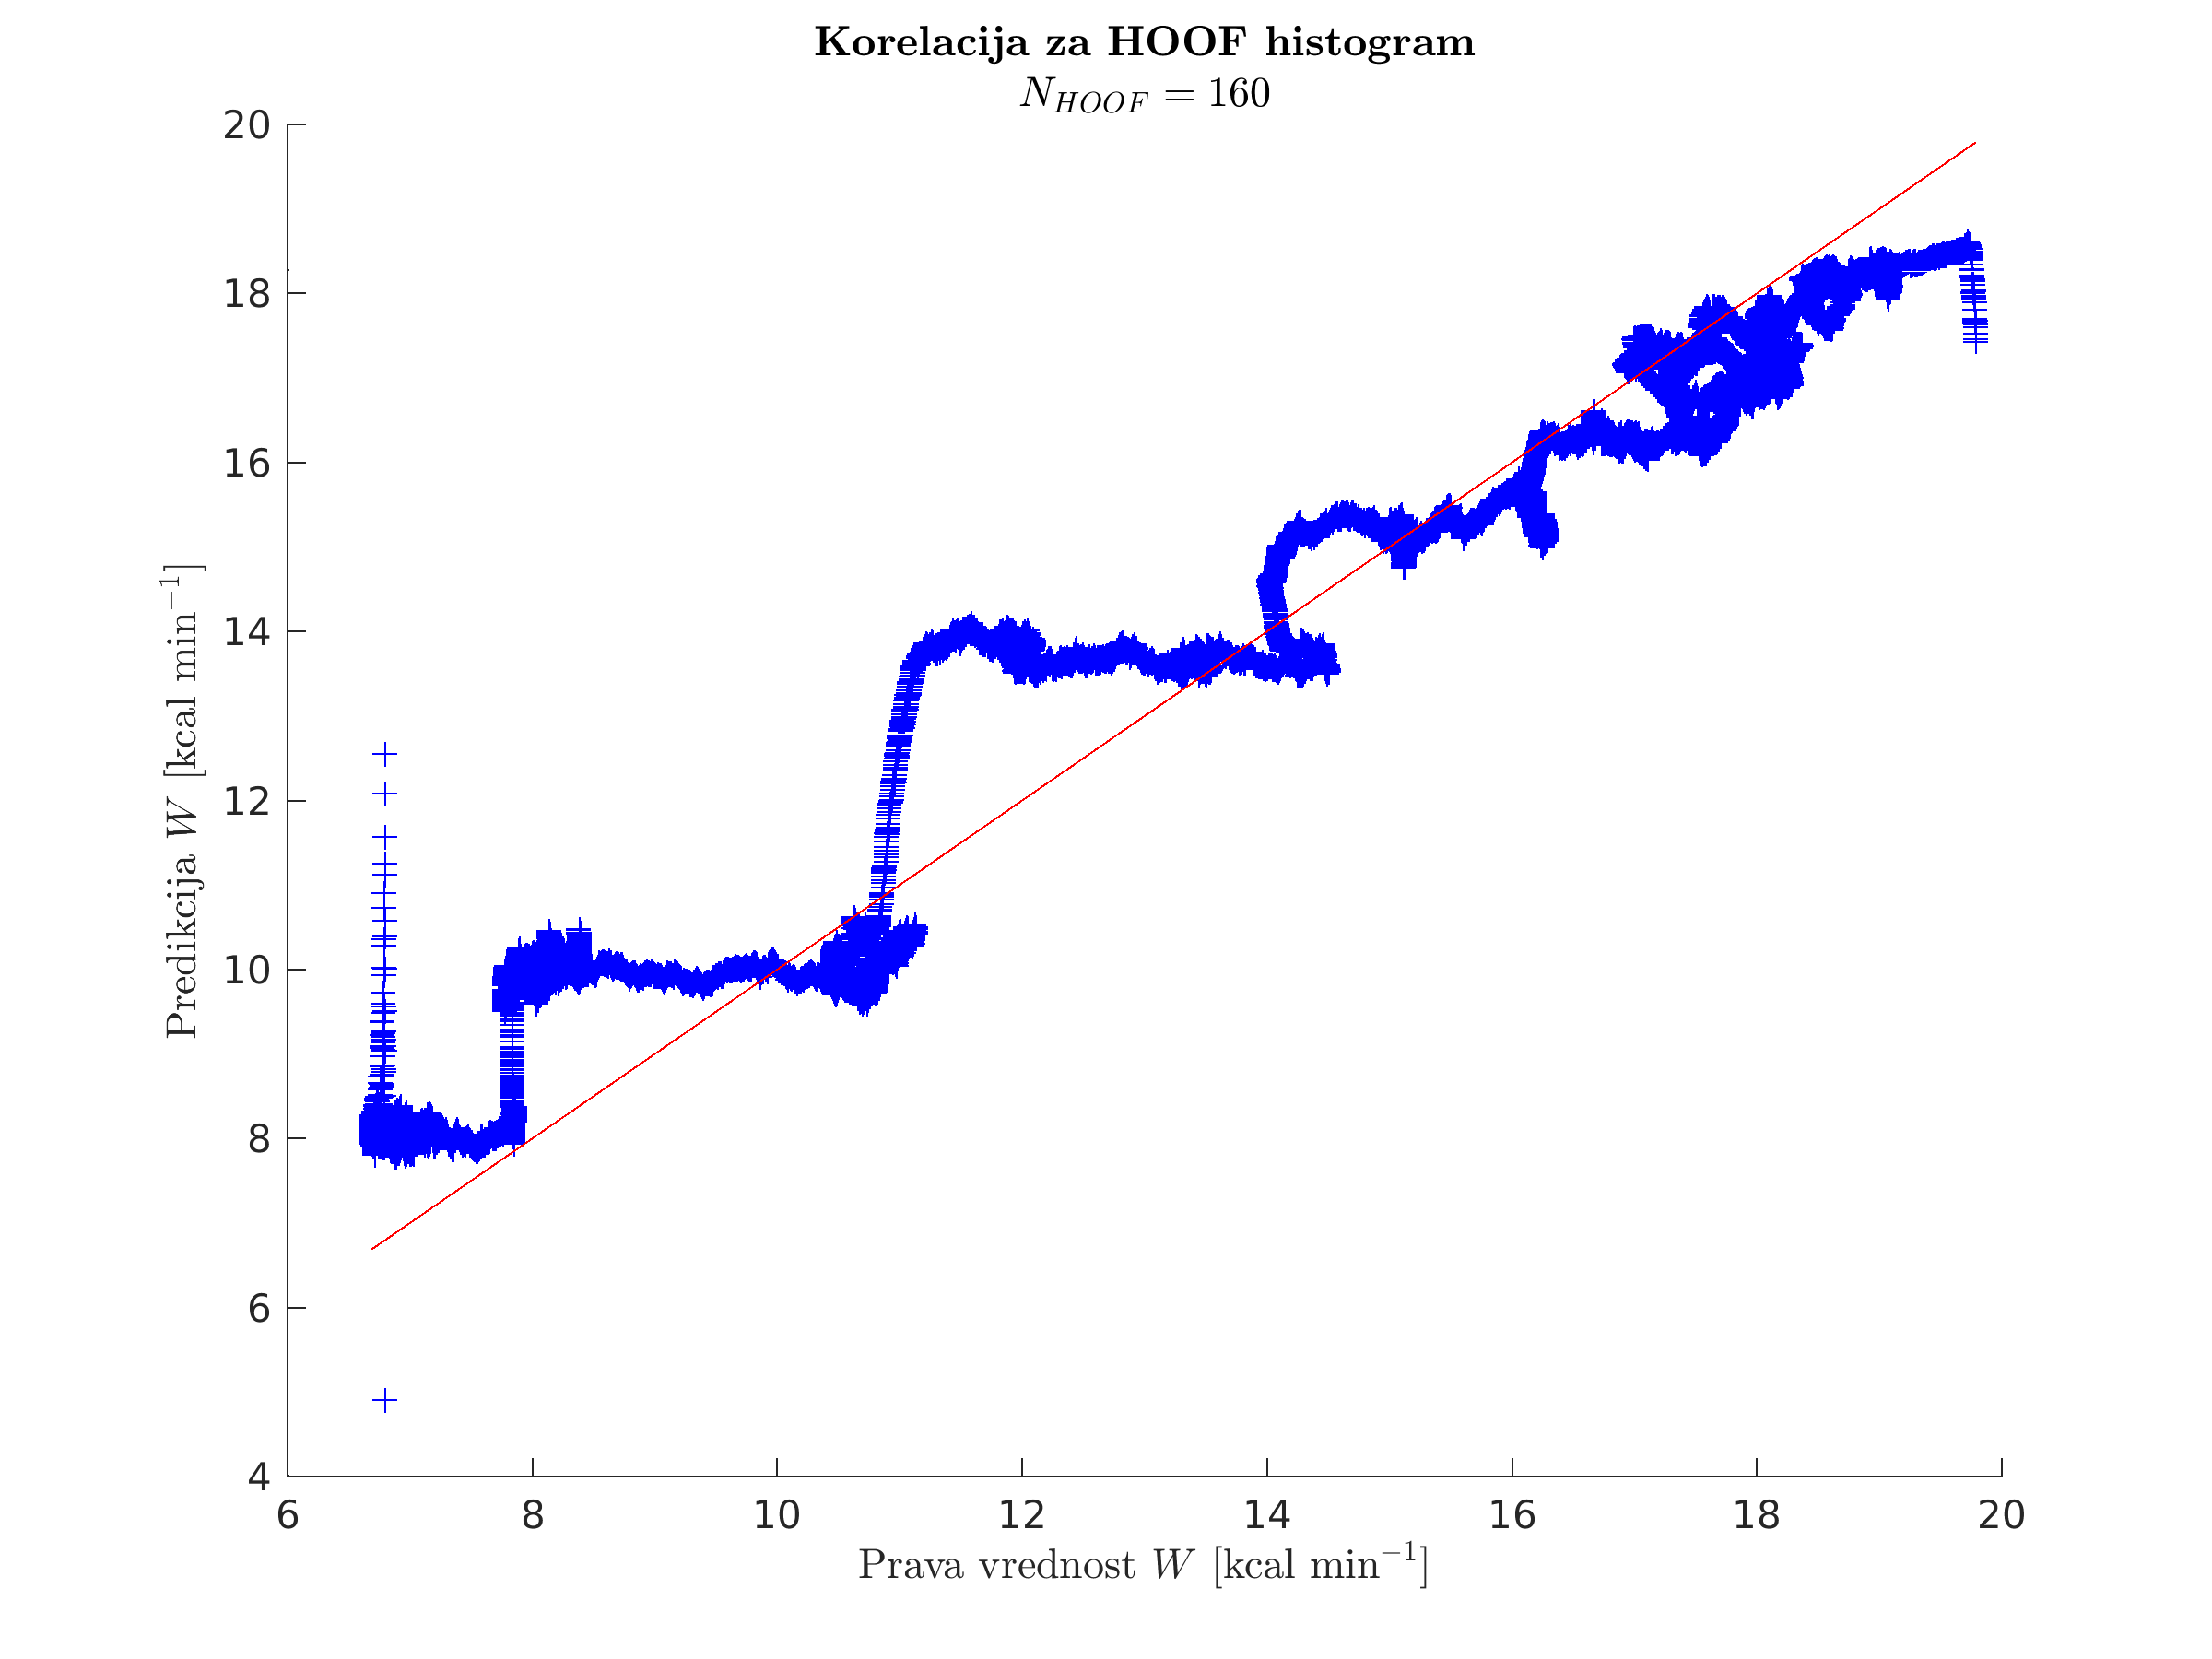
\includegraphics[width=\columnwidth]{./Slike/corr-hafa-160.png}
      \caption{Korelacija $N_{HAFA}=160$.}
      \label{fig:corr-hafa-160}
    \end{subfigure}
    \caption[Grafi korelacij modelov z različnim $N_{HAFA}$]{Grafi korelacij modelov z različnim številom stolpcev $N_{HAFA}$ HAFA deskriptorja. Rezultati so si zelo podobni.}
    \label{fig:corr-hafa}
\end{figure}





\subsubsection{Izbira deskriptorjev}

Chaudhry et al. \cite{chaudhry2009histograms} predlaga uporabo histogramov orientiranega optičnega toka (HOOF) za estimacijo gibanja. Vendar pa smo v preliminarnih terenskih testiranjih \cite{koporec2017observation} ugotovili, da njihova uporaba v realnih okoliščinah ni zadovoljiva. HOOF deskriptorju smo pripeli HAFA deskriptor in tako dobili razširjeni deskriptor HOOF-HAFA, ki v splošnem daje boljše rezultate, kot lahko vidimo v tabeli \ref{tab:izbira} in na primerjalnih slikah \ref{fig:izbira}.

Pri evaluaciji deskriptorjev HOOF in HOOF-HAFA smo uporabili učne vzorce hrbtne kamere terenskih testov. Evaluirali smo za podatke srčnega utripa $hr$. Srčni utrip smo za gradnjo modelov pretvorili v energijsko porabo $W$ po enačbi \eqref{eq:charlot}. Pridobljene značilke smo normirali na intervalu [0,1] in jih uporabili za učenje regresijskega modela z metodo podpornih vektorjev $\epsilon$-SVR in jedrom RBF. Za določitev optimalnih parametrov, ki so predstavljeni v tabeli \ref{tab:nhoof-param}, smo uporabili optimizacijsko metodo mrežnega iskanja \cite{hsu2003practical}. Rezultate smo filtrirali še s Gaussovim jedrom (predstavljen v \ref{sec:gaussov-filter}) velikosti $6$ in varianco $\sigma=16$. 

\begin{table}[htb]
	\centering
    \begin{tabular}{l S[table-format=2.3] S[table-format=1.3] S[table-format=1.3] S[table-format=1.3]}
    \toprule
    \textbf{Deskriptor} & \thead{$\mathbf{C}$} & \thead{$\mathbf{\gamma}$} & \thead{$\mathbf{\epsilon}$} & \thead{MSE} \\ 
    \midrule
    HOOF & 2.828 & 11.314 & 0.435 & 2.192 \\
    HOOF-HAFA & 5.657 & 2.828 & 0.154 & 1.781 \\
    \bottomrule
    \end{tabular}
    \caption[Optimalni parameteri RBF jedra modelov za izbiro deskriptorjev]{Optimalni parametri RBF jedra za modele z različnim deskriptorjem.}
    \label{tab:izbira-param}
\end{table}


\begin{table}[htb]
	\centering
    \begin{tabular}{l S[table-format=1.3] S[table-format=1.3] S[table-format=1.3] S[table-format=2.2]}
    \toprule
    \textbf{Deskriptor} & \thead{$\mathbf{r}$} & \thead{RAE} & \thead{RRSE} & \thead{nSV [\%]}\\
    \midrule%nSV
    HOOF & 0.992 & 0.336 & 0.317 & \boldentry{2.2}{82.34} \\%2187/2656
    \textbf{HOOF-HAFA} & \boldentry{1.3}{0.991} & \boldentry{1.3}{0.157} & \boldentry{1.3}{0.205} & 89.53 \\%2378
    \bottomrule
    \end{tabular}
    \caption[Rezultati evaluacije modelov z različnim deskriptorjem]{Rezultati evaluacije modelov z različnim deskriptorjem. Optimalni rezultati so odebeljeni. Vidimo lahko, da se bolje odnese razširjeni deskriptor HOOF-HAFA, čeprav model uporablja več podpornih vektorjev. }
    \label{tab:izbira}
\end{table}



\begin{figure}[htb]
	\centering
    \begin{subfigure}[t]{0.45\columnwidth}
      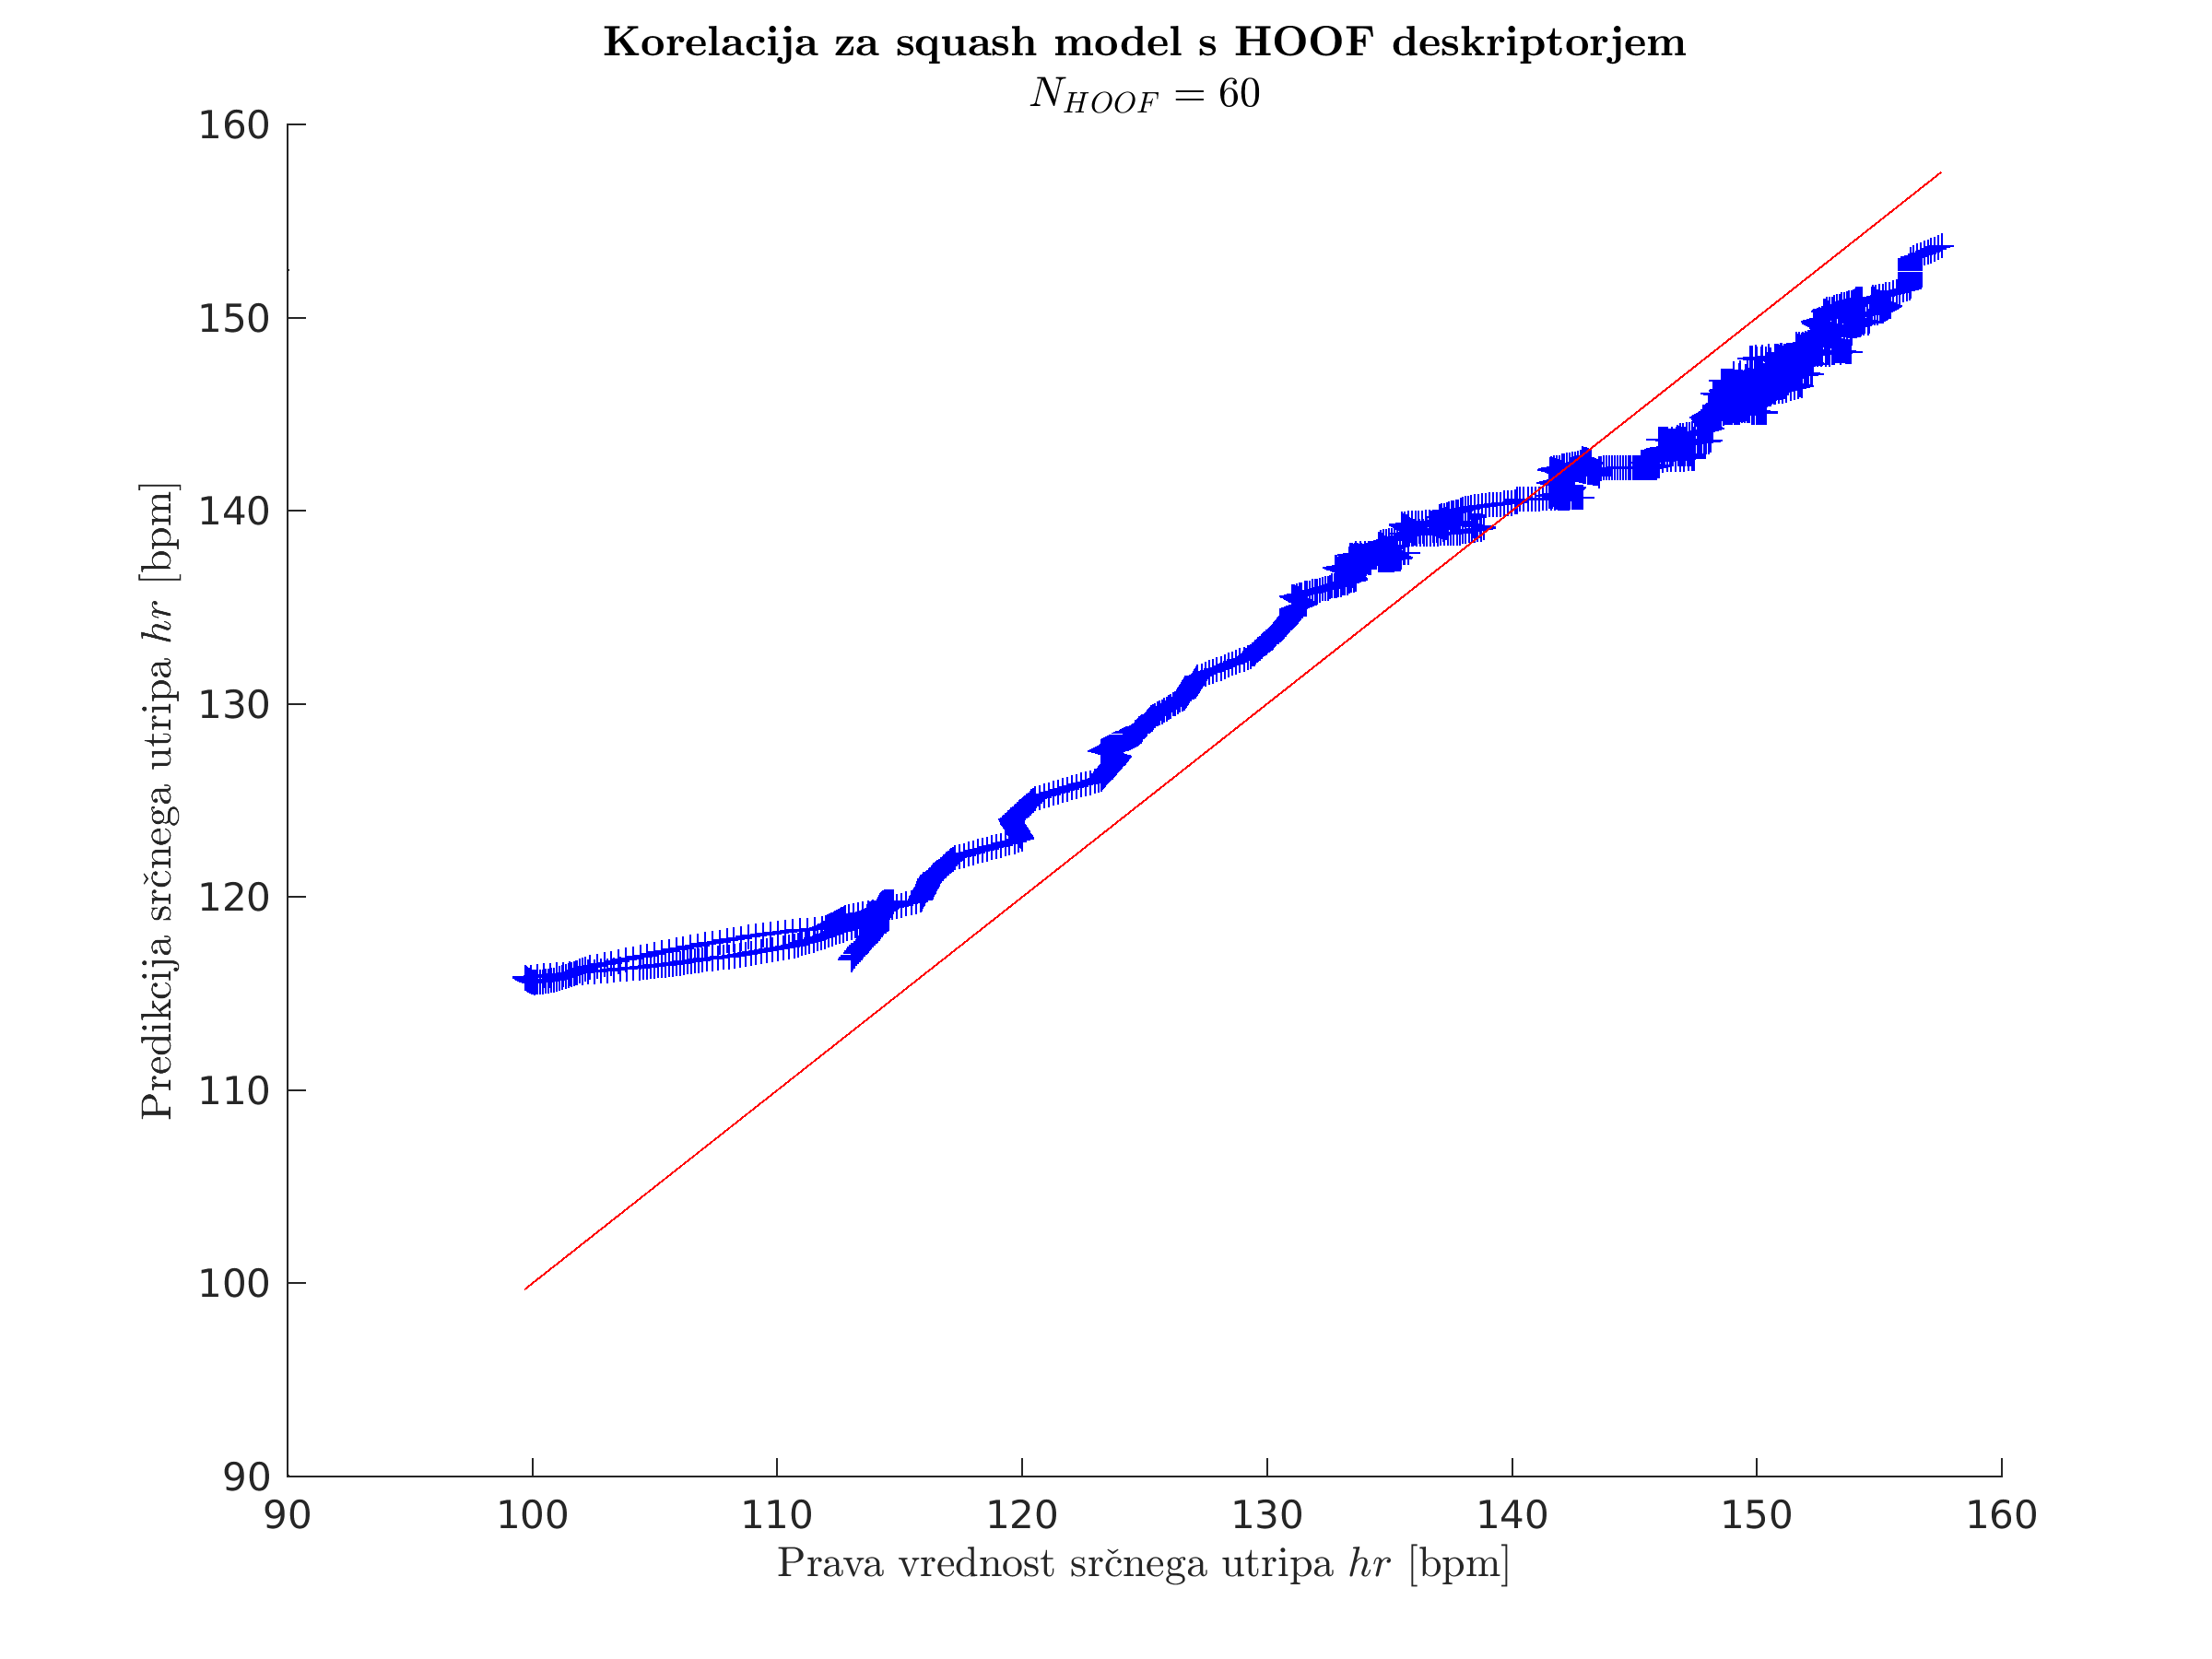
\includegraphics[width=\columnwidth]{./Slike/corr-hoof.png}
      \caption{Korelacija $N_{HOOF}=60$.}
      \label{fig:izbira-hoof}
    \end{subfigure}
    ~
    \begin{subfigure}[t]{0.45\columnwidth}
      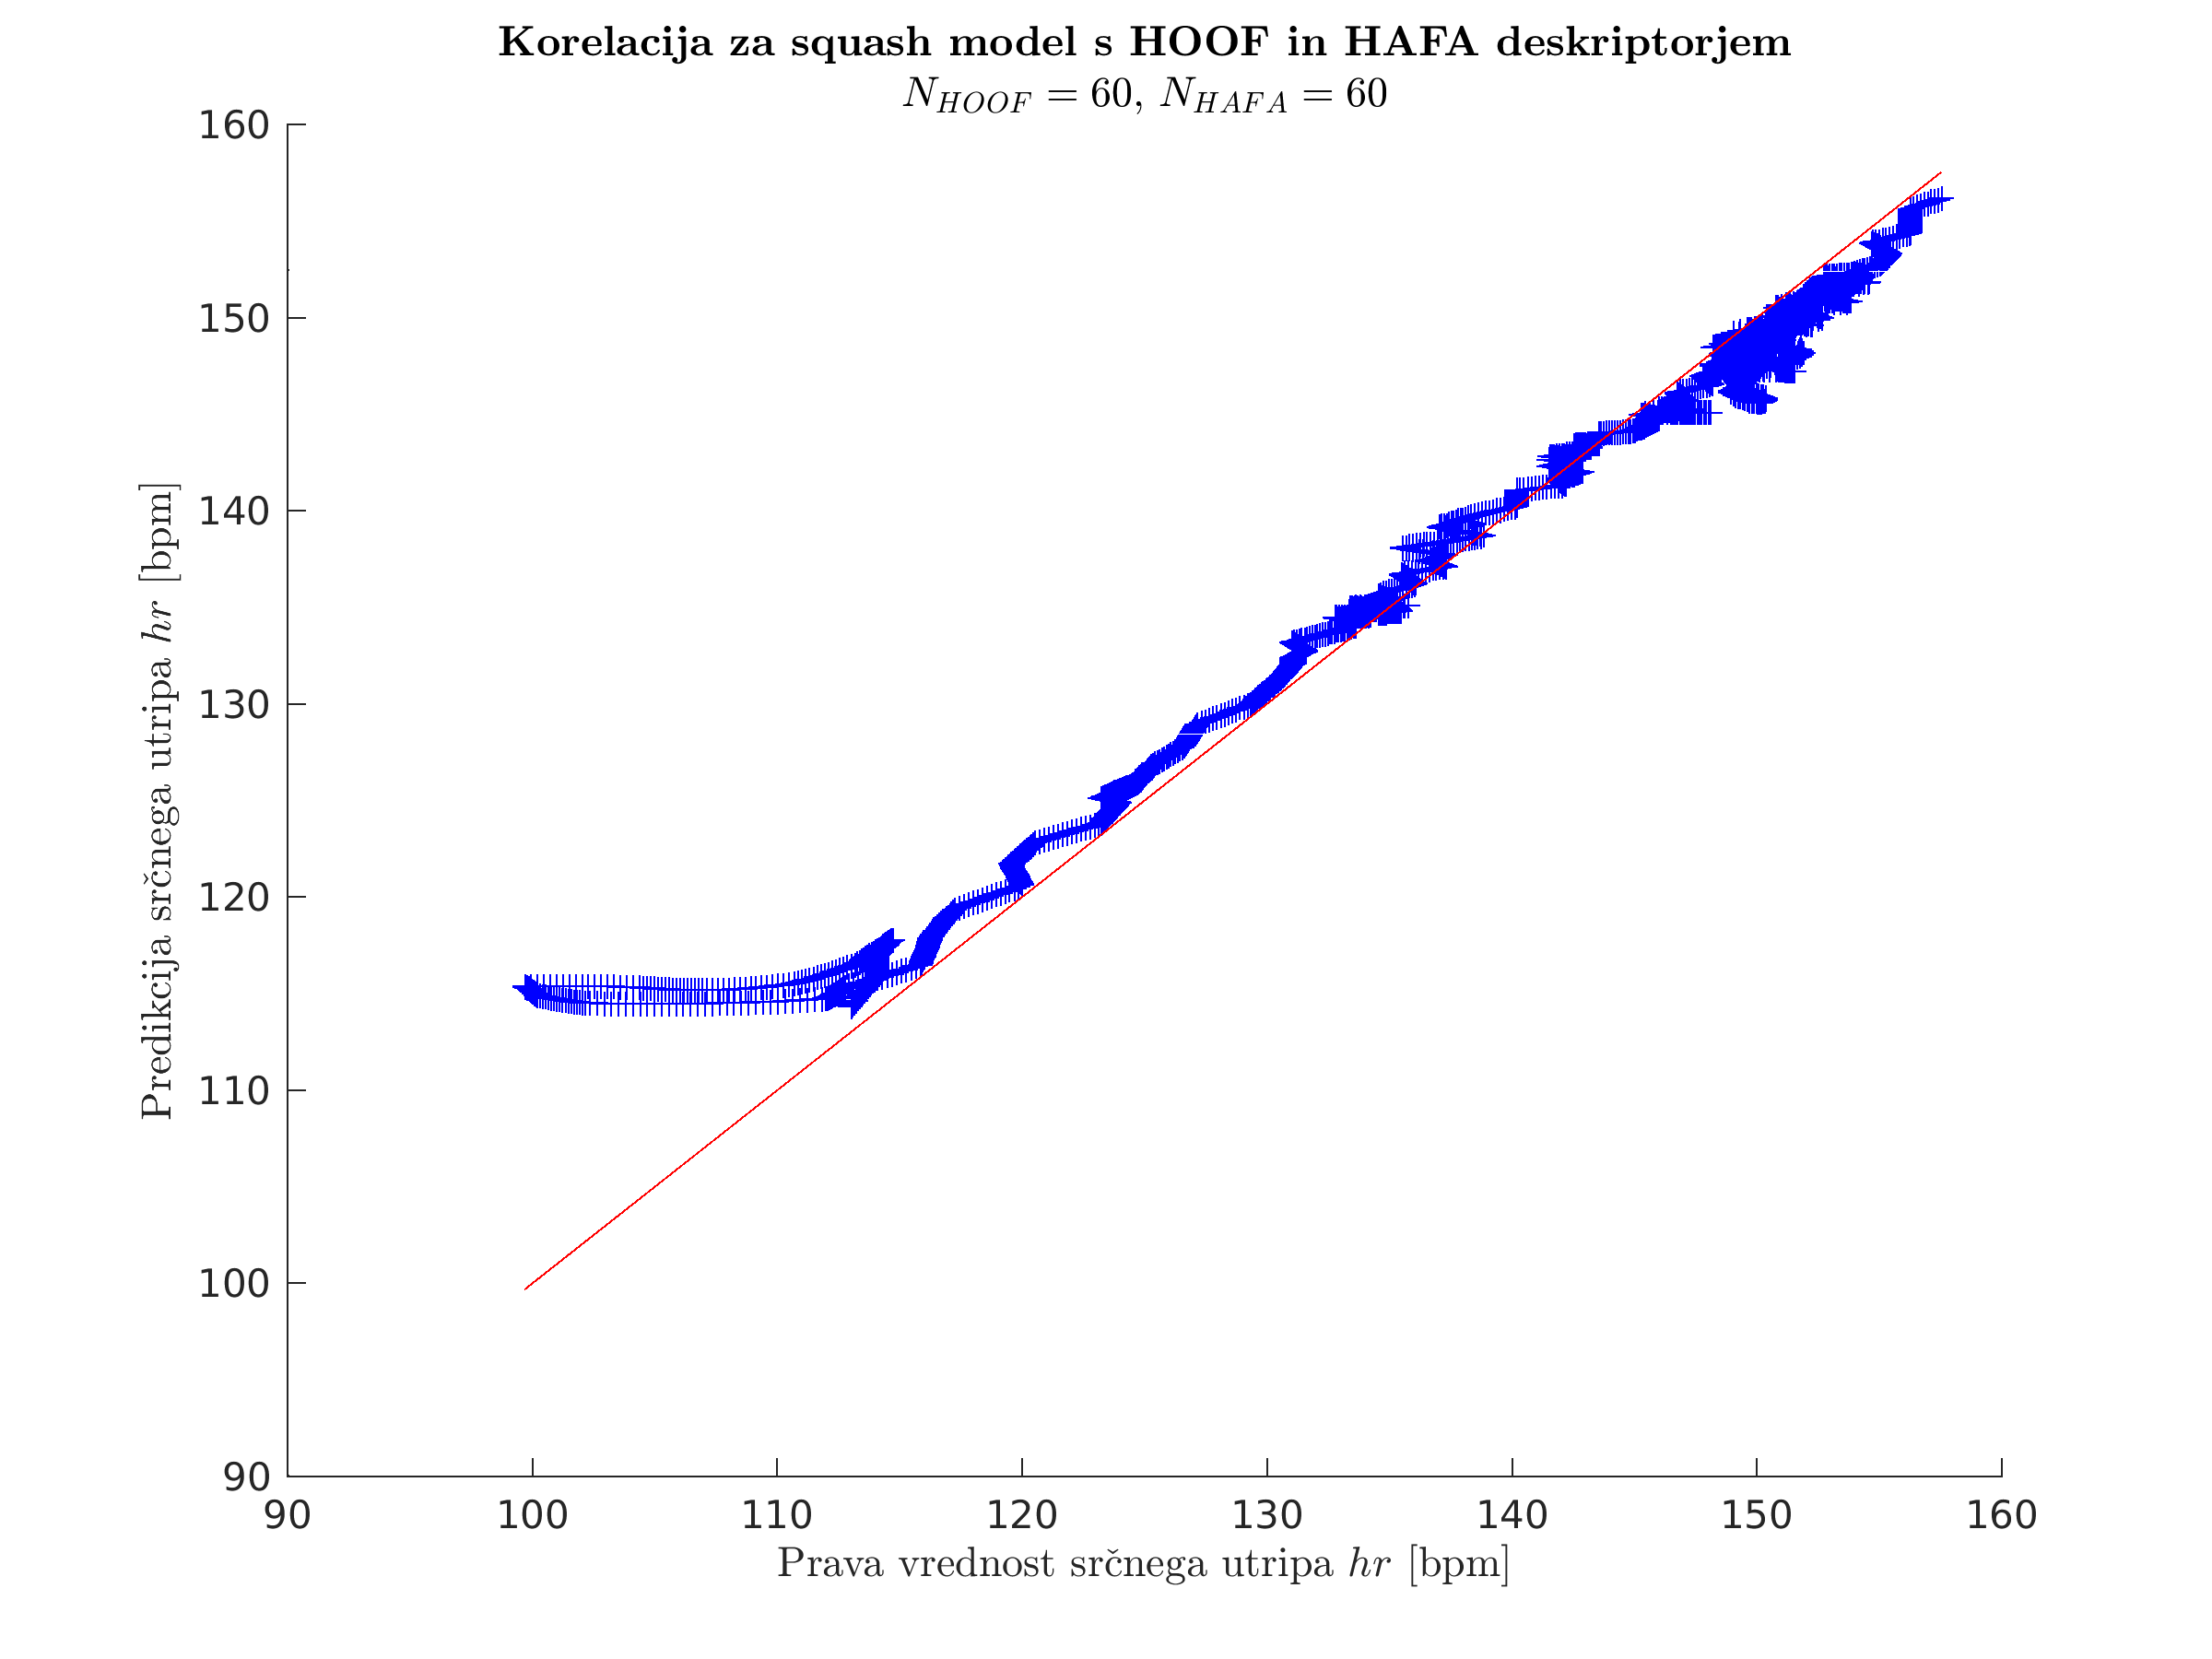
\includegraphics[width=\columnwidth]{./Slike/corr-hoof-hafa.png}
      \caption{Korelacija $N_{HOOF}=60$,\\$N_{HAFA}=60$.}
      \label{fig:izbira-hoofhafa}
    \end{subfigure}
    \caption[Primerjava modelov s HOOF in HOOF-HAFA deskriptorji]{Primerjava grafov korelacij modelov z različnimi deskriptorji. Model \subref{fig:izbira-hoof}) smo naučili s HOOF deskriptorjem. Model \subref{fig:izbira-hoofhafa}) smo naučili s HOOF in HAFA deskriptorjem. Posamezen vzorec je tako vseboval $120$ značilk. Pri primerjavi korelacije lahko opazimo vidno razliko. Model \subref{fig:izbira-hoofhafa}) dokazuje, da je razširjeni deskriptor boljši.}
    \label{fig:izbira}
\end{figure}













\subsection{Testiranje sledilnikov za optični tok}\label{sec:testiranje-sledilnikov-za-opticni-tok}
Sledilnike smo testirali na sekvencah slik \textit{handball1} in \textit{handball2} podatkovne baze VOT2016 \cite{kristan2016visual}. Sledila je še hitra vizualna ocena delovanja na kratkih izsekih video posnetka \cite{squashtv2014squash}.

Pri testiranju sekvenc slik podatkovne baze VOT2016 smo poenostavili rotirajoča referenčna področja detekcij na nerotirajoča področja. Pri tem smo za zgornji levi kot $T_0(x,y)$ in spodnji desni kot $T_1(x,y)$ uporabili enačbo \eqref{eq:vot-bb}, kjer so $\left( x_i, y_i\right), \forall i=1,\ldots,4$ ogljišča rotirajočega referenčnega področja. 

\begin{equation}
\begin{aligned}
	T_0(x,y) &= \left( \min_{i = 1,\ldots,4}\left\{x_i \right\}, 
    \min_{i=1,\ldots,4}\{y_i \} \right) \\
    T_1(x,y) &= \left( \max_{i = 1,\ldots,4}\left\{x_i \right\}, 
    \max_{i=1,\ldots,4}\{y_i \} \right)
\end{aligned}
\label{eq:vot-bb}
\end{equation}

Ker je za naš sledilnik najbolj pomembno zanesljivo delovanje, smo izbrali mero prekrivanja področja.


Video posnetek \cite{squashtv2014squash} smo za potrebe vizualne ocene delovanja na squash posnetkih razdelili na več kratkih izsekov. Pri tem smo uporabili le hrbtne posnetke mirujoče kamere. 

Rezultati testiranja so prikazani v tabeli \ref{tab:region-overlap}. Za izbrane sledilnike smo določili povprečje prekrivanja področja za posamezen posnetek. V tretjem stolpcu je predstavljeno povprečje prekrivanja glede na oba posnetka. Najboljši rezultati so odebeljeni. Po tabeli \ref{tab:region-overlap} se za posnetek \textit{handball1} najbolje izkaže CORR sledilnik. Za posnetek \textit{handball2} smo dobili najboljše rezultate pri sledilniku OPENCV-TLD. V povprečju se najbolje izkaže sledilnik CORR.




\begin{table}[htb]
	\centering
    \begin{tabular}{l S[table-format=1.3] S[table-format=1.3] S[table-format=1.3]}
    \toprule
    \textbf{Sledilnik} & \thead{$\mathbf{\Phi(\mathrm{handball1})}$} & \thead{$\mathbf{\Phi(\mathrm{handball2})}$} & \thead{$\mathbf{\overline{\Phi}}$}  \\
    \midrule%nSV
    NEBEHAY-TLD & 0.035 & 0.130 & 0.083 \\
    CCV-TLD & 0.117 & 0 & 0.117 \\
    OPENCV-TLD & 0.002 & \boldentry{1.3}{0.178} & 0.09 \\
    CORR & \boldentry{1.3}{0.214} & 0.160 & \boldentry{1.3}{0.187} \\
    \textbf{KCF} & {0.161} & {0.166} & {0.164} \\
    \bottomrule
    \end{tabular}
    \caption[Povprečje prekrivanja področja za posamezen sledilnik]{Povprečje prekrivanja področja za posamezen sledilnik in posnetek. V tretjem stolpcu je predstavljeno povprečje prekrivanja glede na oba posnetka. Najboljši rezultati so odebeljeni. Po tabeli \ref{tab:region-overlap} se za posnetek \textit{handball1} najbolje izkaže CORR sledilnik. Za posnetek \textit{handball2} smo dobili najboljše rezultate pri sledilniku OPENCV-TLD. V povprečju se najbolje izkaže sledilnik CORR.}
    \label{tab:region-overlap}
\end{table}


Na sliki \ref{fig:tracker-visual} lahko vidimo primer delovanja sledilnikov za oba posnetka. Referenčni igralec, ki mu morajo slediti ima rumeno majico. Za posnetek \textit{handball1} je predstavljena 15. slika, za posnetek \textit{handball2} pa 111. slika. Rezultati v tabeli \ref{tab:region-overlap} se skladajo z opažanji na sliki \ref{fig:tracker-visual}.

\begin{figure}[htb]
\centering

	\begin{subfigure}[t]{0.45\columnwidth}
      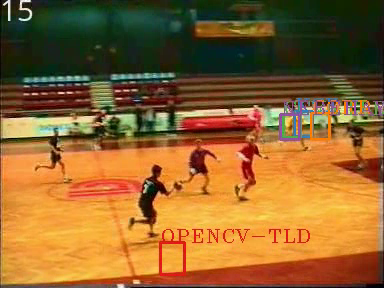
\includegraphics[width=\columnwidth]{./Slike/handball1-example.png}
      \caption{15. slika posnetka \textit{handball1}.}
      \label{fig:handball1}
    \end{subfigure}
    ~
    \begin{subfigure}[t]{0.45\columnwidth}
      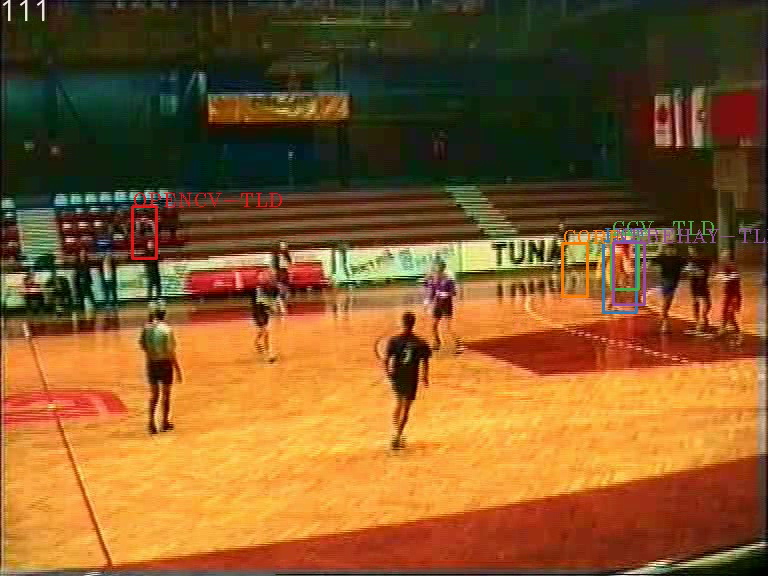
\includegraphics[width=\columnwidth]{./Slike/handball2-example.png}
      \caption{111. slika posnetka \textit{handball2}.}
      \label{fig:handball2}
    \end{subfigure}  
\caption[Primer delovanja sledilnikov za \textit{handball} posnetke]{Primer delovanja sledilnikov za \textit{handball} posnetke. Referenčni igralec, ki mu morajo slediti ima rumeno majico. }
\label{fig:tracker-visual}
\end{figure}




Čeprav smo z mero določili, da se je najbolje izkazal sledilnik CORR, se je pri hitri vizualni oceni sledenja na izsekih posnetka \cite{squashtv2014squash} izkazalo, da najbolje deluje sledilnik KCF. Primer boljšega delovanja KCF sledilnika je slika \ref{fig:squash-tracker-visual}, kjer sledimo modremu igralcu. Na isti sliki posnetka je KCF algoritem našel modrega igralca, medtem ko ga je CORR algoritem zamenjal z drugim igralcem. 



\begin{figure}[htb]
\centering

	\begin{subfigure}[t]{0.45\columnwidth}
      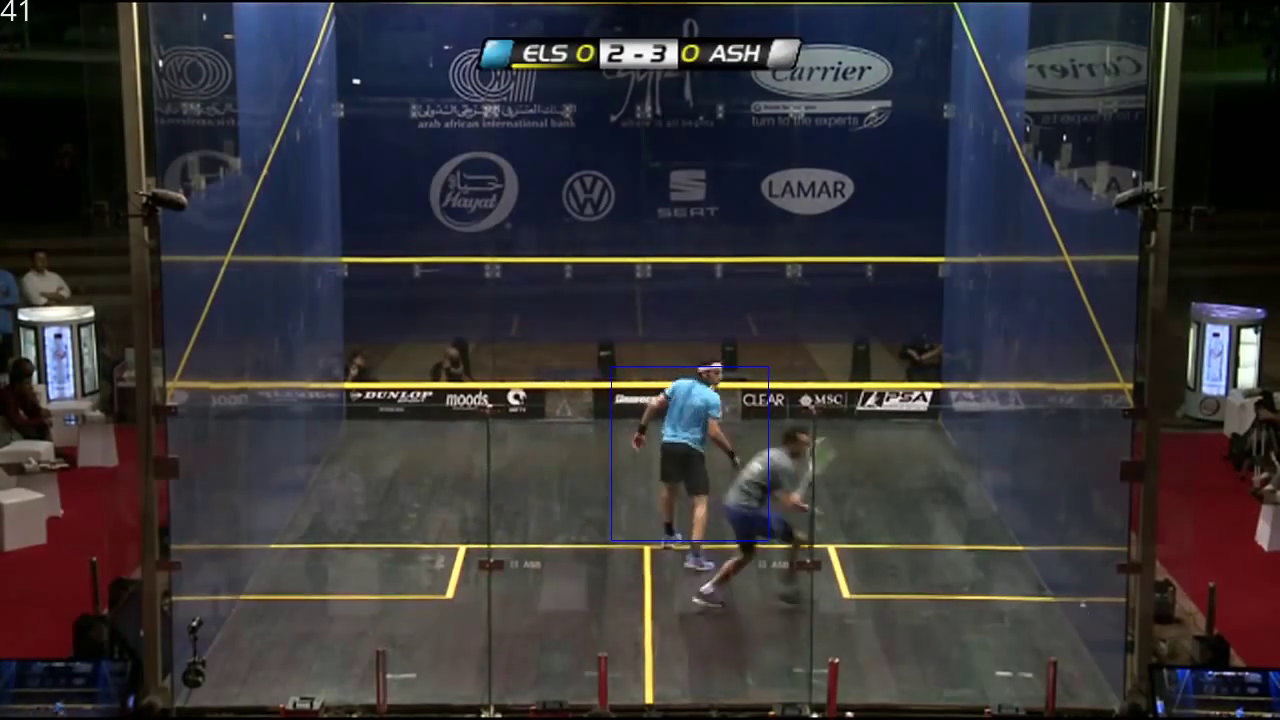
\includegraphics[width=\columnwidth]{./Slike/squash-1-kcf-example.png}
      \caption{41. slika posnetka \cite{squashtv2014squash} s KCF sledilnikom.}
      \label{fig:squash-1-kcf}
    \end{subfigure}
    ~
    \begin{subfigure}[t]{0.45\columnwidth}
      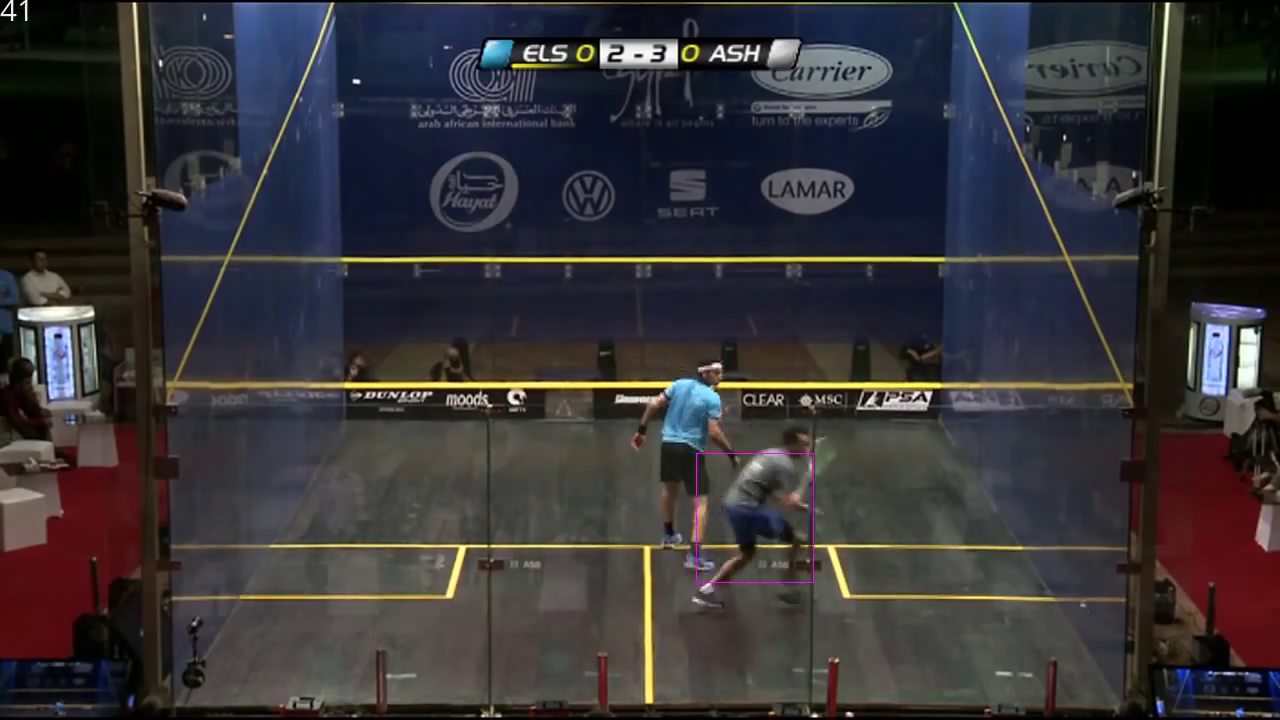
\includegraphics[width=\columnwidth]{./Slike/squash-1-corr-example.png}
      \caption{41. slika posnetka \cite{squashtv2014squash} s CORR sledilnikom.}
      \label{fig:squash-1-corr}
    \end{subfigure}  
\caption[Primer delovanja sledilnikov za squash posnetek]{Primer delovanja sledilnikov za squash posnetek. Gre za identični sliki posnetka, pri čemer smo na sliki \ref{fig:squash-1-kcf} uporabili KCF algoritem, na sliki \ref{fig:squash-1-corr} pa CORR algoritem. Sledilnika sta morala slediti igralcu z modro majico.}
\label{fig:squash-tracker-visual}
\end{figure}


Boljše delovanje KCF je razumljivo, saj prvi testi temeljijo na posnetkih rokometa, drugi pa na squashu, kjer gre za bistveno drugačno igro. Če pogledamo tabelo \ref{tab:region-overlap} ima KCF drugo najboljše povprečje, prav tako pa so si rezultati posameznih posnetkov zelo podobni. 









\subsection{Združevanje slik iz dveh Kinect kamer}\label{sec:zdruzevanje}
\subsubsection{Združevanje z značilkami}
Časovno sinhornizirana zaporedja slik smo nato poskušali združiti z metodo panoramskega šivanja slik z uporabo značilk, kot je opisano v delu \cite{brown2007automatic}. Tu smo namesto SIFT značilk uporabili SURF značilke.
Združevanje s značilkami se ni obneslo, zato smo to metodo opustili. Primer neuspelega poskusa je prikazan na sliki \ref{fig:zdruzevanje-znacilke}.

\begin{figure}[htb]
\centering
\begin{subfigure}[t]{0.45\columnwidth}
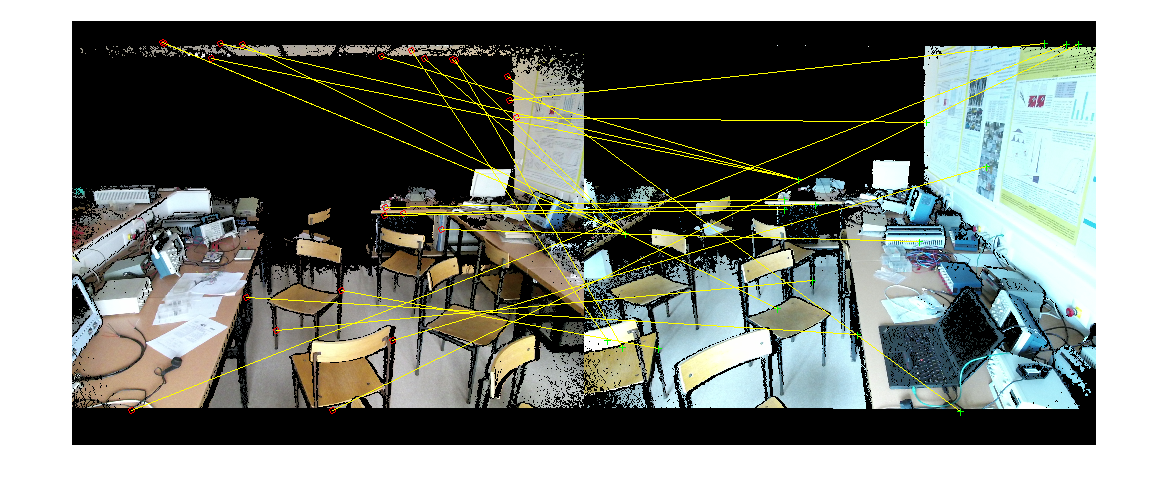
\includegraphics[width=\columnwidth]{./Slike/matched-features.png}
\caption{Ujemajoče SURF značilke}
\label{fig:zdruzevanje-surf}
\end{subfigure}
~
\begin{subfigure}[t]{0.45\columnwidth}
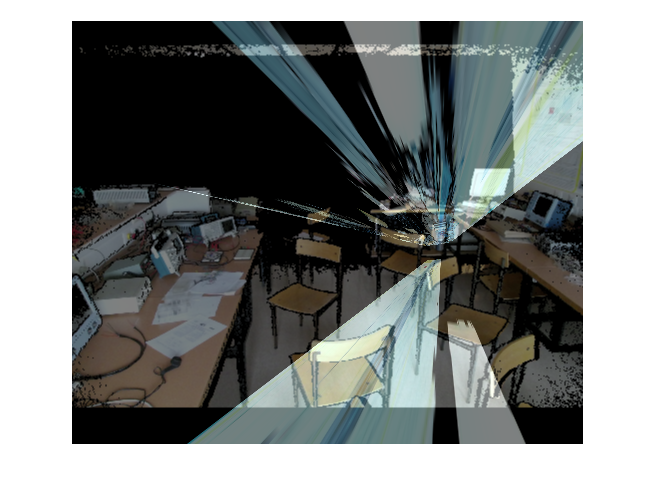
\includegraphics[width=\columnwidth]{./Slike/features-calibration-result.png}
\caption{Rezultat združevanja z značilkami}
\label{fig:zdruzevanje-result}
\end{subfigure}
\caption{Primer neuspelega poskusa združevanja slik iz dveh Kinect kamer s SURF značilkami.}
\label{fig:zdruzevanje-znacilke}
\end{figure}

\subsubsection{Združevanje s kontrolnimi točkami}
Zaporedja slik smo poskušali združiti z ročnim določevanjem kontrolnih točk. Rezultat je bil boljši od združevanja z značilkami, vendar še vedno slab, zato smo tudi to metodo opustili. Primer neuspelega poskusa je prikazan na sliki \ref{fig:zdruzevanje-cp}.

\begin{figure}[htb]
\centering
\begin{subfigure}[t]{0.45\columnwidth}
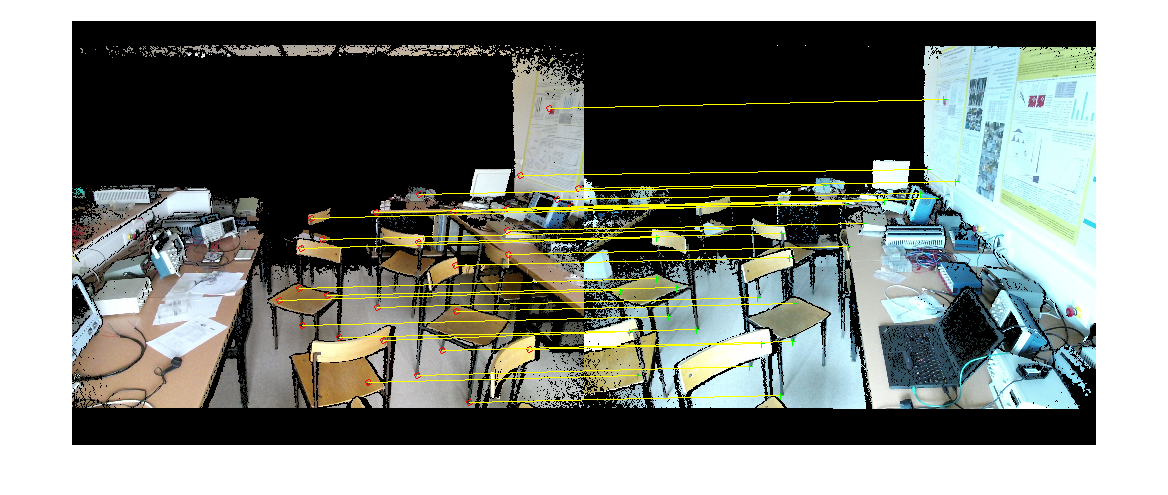
\includegraphics[width=\columnwidth]{./Slike/matched-points.png}
\caption{Ujemajoče kontrolne točke}
\label{fig:zdruzevanje-ujemajoce-cp}
\end{subfigure}
~
\begin{subfigure}[t]{0.45\columnwidth}
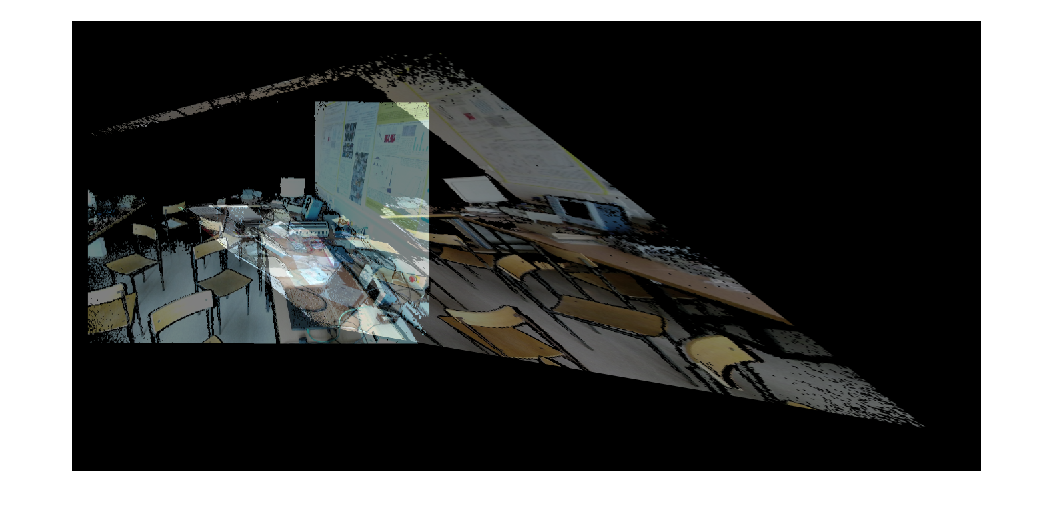
\includegraphics[width=\columnwidth]{./Slike/points-calibration-result.png}
\caption{Rezultat združevanja s kontrolnimi točkami}
\label{fig:zdruzevanje-result-cp}
\end{subfigure}
\caption{Primer neuspelega poskusa združevanja slik iz dveh Kinect kamer s kontolnimi točkami.}
\label{fig:zdruzevanje-cp}
\end{figure}


\subsubsection{Prilagojeno združevanje}
Zaradi nezadovoljivih rezultatov klasičnih metod združevanja stereo slik, smo razvili metodo, ki je prilagojena za Kinect kamere. Iz kamer smo pridobili intrinzične parametre infra-redečega (IR) senzora, in sicer: slikovni koordinati goriščne razdalje $f_u$ in $f_v$ ter slikovni koordinati optičnega središča slike (ang. principal point) $c_u$ in $c_v$. Intrinsične parametre smo uporabili za določitev intrizične matrike $\vec{M}_{int}$ po enačbi \eqref{eq:intrinsic}.


Ker pravih ekstrinsičnih parametrov kamer nismo poznali, smo jih le ocenili z metodo določevanja sečišča vidnih polj obeh kamer. Sečišče je prikazano kot rdeča linija na sliki \ref{fig:zdruzevanje}. S to metodo smo določili translacijski vektor $\vec{t} = \left [ t_x~ t_y~ t_z \right]^\top$ in rotacijsko matriko $\vec{R}$ iz Eulerjevih kotov.

S sledenjem igralca z DS-KCF algoritmom, smo s pomočjo projekcijske matrike \eqref{eq:projection-matrix} določili center tarče v metričnih enotah za vsako sliko zaporedja leve in desne kamere. Kadar slikovni element ni vseboval podatkov globine, smo za center tarče izbrali najbližji slikovni element z veljavno globino.

Prva slika združenega zaporedja je bila slika kamere, kjer se igralec prvič pojavi. Nadaljne slike smo izbirali med zaporedjema kamer glede na pozicijo centra tarče. Ko je šel center tarče skozi upragovljeno mejo, ki je na sliki \ref{fig:zdruzevanje} prikazana z modro linijo smo preklopili na drugo kamero. Razdalja med pragom in sečiščem je znašala \SI{200}{mm}.


\begin{figure}[htb]
\centering
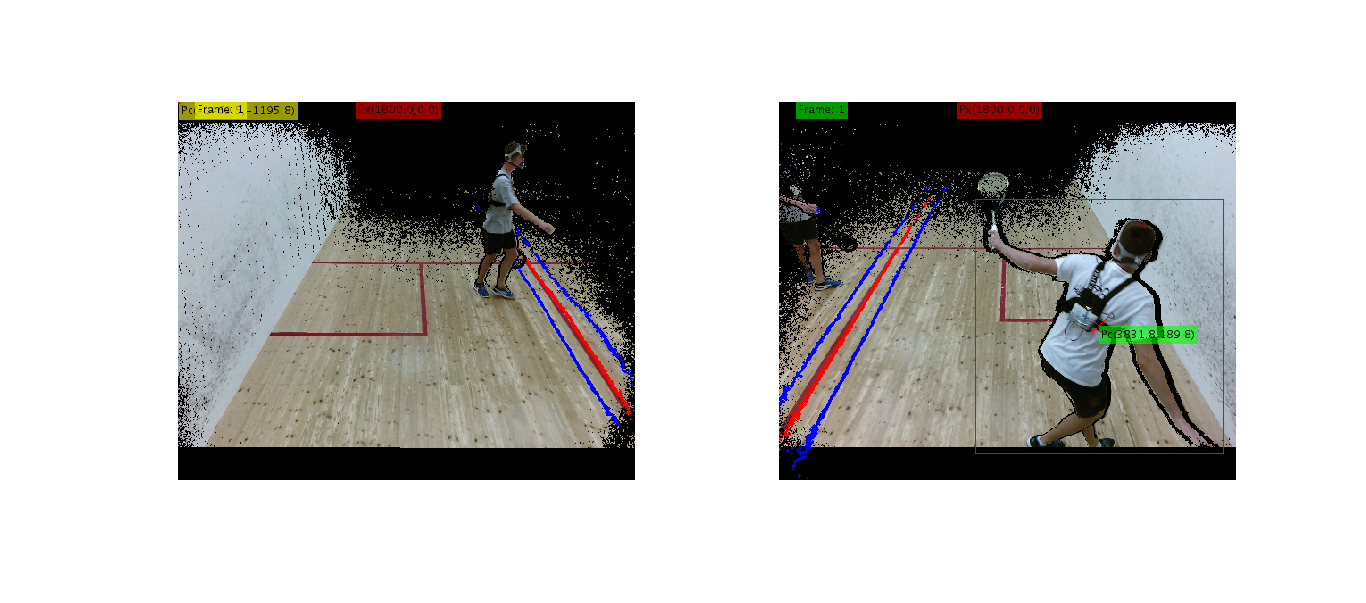
\includegraphics[width=\columnwidth]{./Slike/zdruzevanje-example.png}
\caption[Določevanje sečišča vidnih polj leve in desne Kinect kamere]{Določevanje sečišča vidnih polj leve in desne Kinect kamere. Na sliki sta prikazani prvi sliki zaporedja leve in desne Kinect kamere 1. seta 2. igre terenskega eksperimenta iz 2. faze. Označen je 4. igralec. Zelena barva koordiat središča tarče predstavlja izbrano kamero. Kamera z rumeno barvo ni izbrana. Sečišče je rdeča linija. Modri liniji sta pragova za preklop med kamerama. Ležita \SI{200}{mm} levo in desno od sečišča.}
\label{fig:zdruzevanje}
\end{figure}



















\section{Eksperimenti 1. faze}

\subsection{Določevanje zakasnitve fiziološkega odziva}

We explored the problem of the lag in physiological response as well. Based on Figure \ref{fig:zakasnitev}, we found out that between the change in speed of the treadmill and change of the selected physiological parameter there is a delay. This is perfectly acceptable due to the nature of physiological processes. We found out that offset for heart rate is amounted to \SI{15}{\s} and for energy expenditure to \SI{55}{\s}. Offset was included in models with the \textit{lag} abbreviation.

\begin{figure}[htb]
\centering
\begin{subfigure}[t]{0.45\columnwidth}
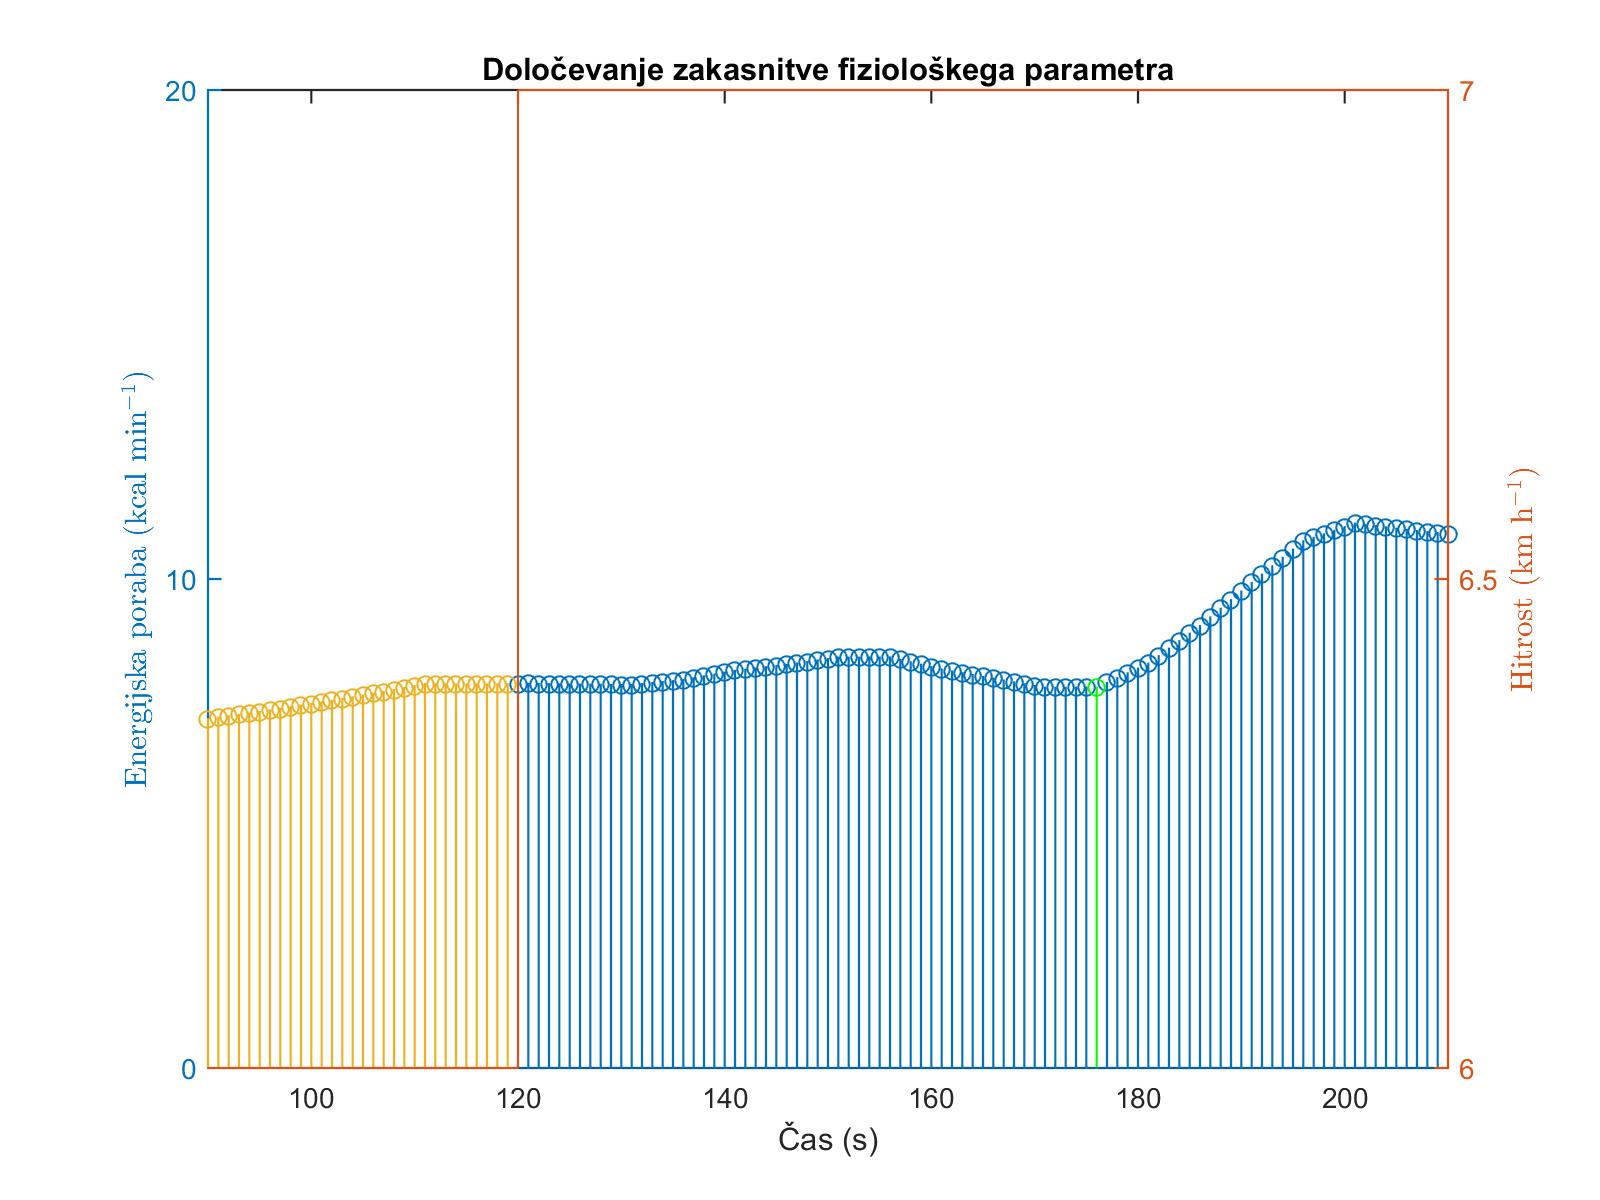
\includegraphics[width=\columnwidth]{./Slike/lag-estimation-train-eem.png}
\caption{Zakasnitev za energijsko porabo.}
\label{fig:lag-estimation-train-eem}
\end{subfigure}
~
\begin{subfigure}[t]{0.45\columnwidth}
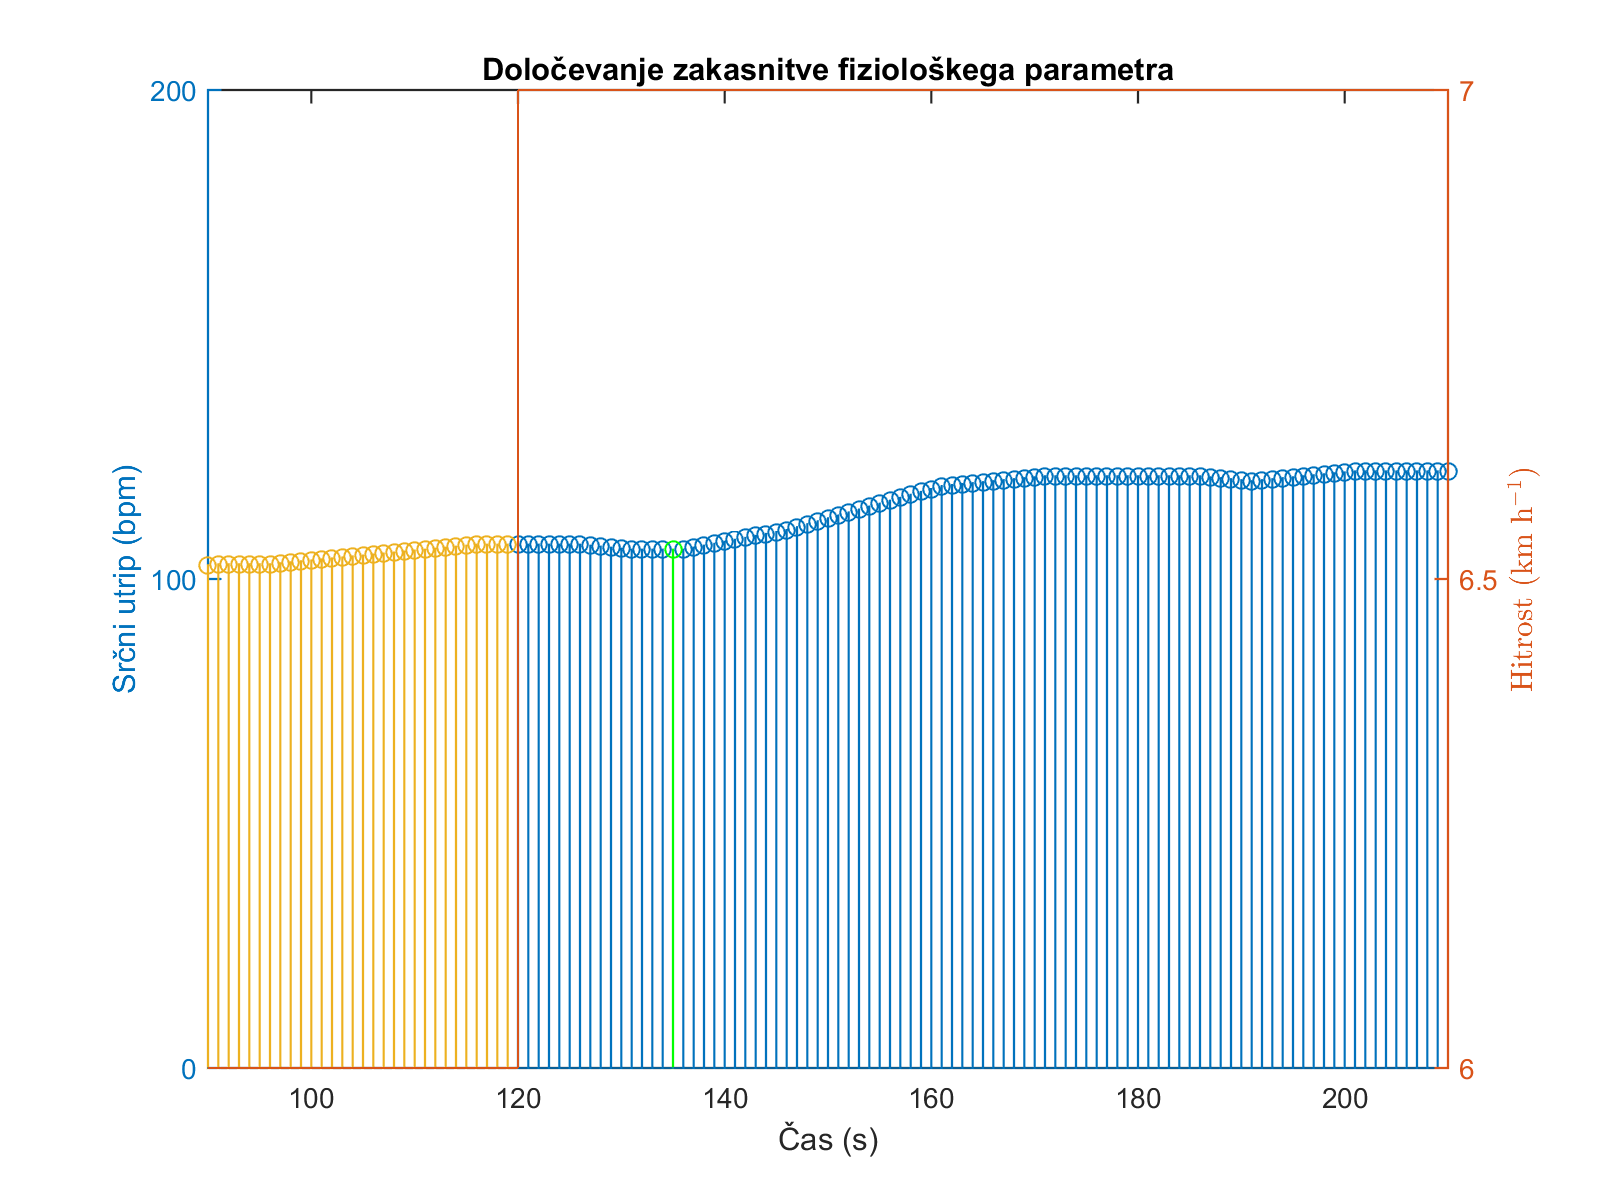
\includegraphics[width=\columnwidth]{./Slike/lag-estimation-train-hr.png}
\caption{Zakasnitev za srčni utrip.}
\label{fig:lag-estimation-train-hr}
\end{subfigure}
\caption{}
\label{fig:lag-estimation-stage1}
\end{figure}


\subsubsection{Normalizacija HAFA deskriptorjev}
% Zakaj naj bi bila ta rešitev dobra
% teorija tovrstne kalibracije
% Kako s to kalibracijo nismo popravili stvari
% In da smo ugotovili da obstaja še prostorski tok, ki bi nam rešil težave
!!!!!!!!!!!!!!!!!!!!!!!!!!!!!!!

V praksi se pokaže, da normiran HAFA histogram ne... -> To paše pod eksperimente.

!!!!!!!!!!!!!!!!!!!!!!!!!!!!!!!!!!!!!!!!!


\subsection{Treadmill experiment}
The first set of experiments was performed in physiological laboratory, with subject running on a treadmill in the presence of the operator---a doctor, who determined the intensity and duration of workload. Heart rate and energy expenditure were measured for an athlete (age: 26 years, height: \SI{177}{\cm}, weight: \SI{79.1}{\kg}, $VO_2max$: \SI{3705}{\ml\per\min}). Energy expenditure was measured using indirect calorimetry with Cosmed CPET Metabolic Cart. System allows breath-by-breath measurement \cite{beaver1973line}. We used Hans Rudolph face mask with prescribed minimal VD (dead space).

\subsubsection{Data acquisition}
We filmed the treadmill from the two different angles: the side-view and the back-view. The slope of the treadmill was from \SI{1.5}{\%} to \SI{2}{\%}. We filmed in $480 \times 640$ resolution with a \SI{30}{fps} speed. An example of a recording is shown in Figure \ref{fig:moving-components}(\subref{fig:original-frame}).

\subsubsection{Procedure}
We have made two series of tests with 20 minutes between them. Physiological parameters were sampled every \SI{5}{\s}. In the first series we made 8 tests, where every test lasted for 2 minutes. The treadmill's speed was increased by \SI{1}{\km\per\hour} every test. First test had a speed of \SI{6}{\km\per\hour} and the last a speed of \SI{13}{\km\per\hour}. In the second series we made 3 tests. Every test lasted for 5 minutes. Treadmill's speeds were \SI{7}{\km\per\hour}, \SI{10}{\km\per\hour} and \SI{13}{\km\per\hour}. The first set was used for the acquisition of samples for learning, and the other for testing.

\subsubsection{Processing}
We then calculated the optical flow \cite{farneback2003two} with the help of tracking algorithm described in \ref{sec:tracking}. For optical flow we used the following parameters: pyramid scale \num{0.5}, number of pyramid layers \num{3}, averaging window size \num{15}, number of iterations at each pyramid level \num{3}, size of the pixel neighborhood \num{5} and standard deviation of the Gaussian \num{1.2}. An example of the obtained optical flow is shown in Figure \ref{fig:optical-flow}.

\begin{figure}[!htb]
	\centering
	%\includegraphics[width=0.75\linewidth, frame]{./slike/colored-opticalFlow-frame-150.png}
    \caption{The optical flow for $150^{\mathrm{th}}$ frame of the first test from the first series of shots with color coding legend in the bottom left corner. We are using a standard color coding based on \cite{baker2011database}. The maximum amplitude of the optical flow in this figure is \SI{17}{px}.}
    \label{fig:optical-flow}
\end{figure}

HOOF features were calculated according to the method described in \cite{chaudhry2009histograms}.

The models have been generated with support vector regression \mbox{$\epsilon$-SVR} in LIBSVM library, which is more specifically described in \cite{CC01a}. We used RBF kernel that takes the form \eqref{eq:rbf-kernel}. Kernel and regression parameters were optimized with grid search approach described in \cite{hsu2003practical}. We needed to determine  regression penalty parameter $C > 0$, loss function parameter $\epsilon > 0$, and kernel coefficient $\gamma$. 

\begin{equation} \label{eq:rbf-kernel}
		K(\mathbf{x_i}, \mathbf{x_j}) = e^{
        	-\gamma 
        	\begin{Vmatrix}
        		\mathbf{x_i} - \mathbf{x_j}
        	\end{Vmatrix}^2
        }
\end{equation}
%The optimal parameters for each model are presented in Table \ref{tab:optimalni-parametri}.

We have built \num{8} models, divided into two categories: \textit{hr} models, which predict heart rate and \textit{eem} models, which provide the energy expenditure in \si{\kcal\per\min}.

The models are further divided according to the type of input data. We used a side-view camera (abbreviation \textit{sv}), and the back-view camera (abbreviation \textit{bv}). We extended our experiment by incorporating lag between measurements and reference values. With models, marked as \textit{lag}, we checked the proposed time delay between excitation and physiological response.

In experiments with \textit{mixed} abbreviations, we built the model on the data from the one view, and tested it on the another view.

Additional \textit{mixed} model experiment was generated with data from both cameras, side-view and back-view. Recordings from both cameras were concatenated and cropped. 

\subsection{Object tracking}\label{sec:tracking}
In many sports, there are a number of players participating and therefore they are all visible in each video frame. Necessary component of such system will be a tracking functionality, therefore we ran a tracker on treadmill video to check how the method performs if the position of the player is non-stationary and obtained by the tracking algorithm. Results which included tracking step have \textit{tr} abbreviation. 

For object tracking we used KCF tracking framework implemented in OpenCV because it gave us best results. The tracking method is an implementation of \cite{henriques2012exploiting} which is extended to KCF with color-names features. Extension is based on \cite{danelljan2014adaptive}.

Default parameters for tracking were: Gaussian kernel bandwidth $0.2$, linear interpolation factor for adaptation $0.075$, regularization $0.01$, max patch size $6400$, spatial bandwidth $0.0625$, resize features activated to improve the processing speed, training coefficients splitted into two matrices, wrapping around the kernel values not activated, non-compressed descriptors in gray, compressed descriptors in colornames, the PCA method to compress the features activated, compressed size $2$ and compression learning rate $0.15$.

% Cropal sem sliko optičnega toka.
With KCF tracking framework tracked objects were defined with bounding box. The region of interest, where bounding box was calculated, was set on the first frame of every recording. Bounding box was used to crop the region of interest from optical flow image of particular frame and calculated HOOF features on it. If tracker couldn't find an object---it disappeared from our view or there were technical difficulties to calculate correspondences---bounding box didn't exist and all histogram bins were therefore zero.

Finally, cameras may shake, if held manually. We simulated this scenario by artificially introducing random small displacements and rotation into the video. Every frame was transformed with random Euclidean transformation, where translation was limited to \SI{4}{\%} of frame size and rotation to \SI{0.13}{rad}. Random transformations were smoothed with Kalman filter \eqref{eq:kalman}, where the variance of process noise was \num{2}, the variance of model noise \num{1024} and variance for posteriori error covariance \num{2}. The tracking algorithm was run \emph{after} this motion noise was added, and these results are denoted by \textit{sh} abbreviation.

Comparison between the measured physiological parameters (\SI{5}{\s}) sampling, and our predictions at \SI{30}{fps} required interpolation of physiological parameters, which was performed in Matlab.



\subsection{Denoising the results}

Because of the noisy output of models, we had to filter them with the Kalman filter \cite{forsyth2002computer}. It is represented by the equation  in state space, where state is the state of speed $v$ and acceleration $a$ with unknown input parameters speed $v_n$ and acceleration $a_n$. The initial velocity and acceleration were $0$. Variance of process noise for all models was \num{0.04}. Variance of model noise was \num{456.13}. Due to the unknown initial values, we used variance \num{456.13} for the posteriori error covariance.

\begin{equation} \label{eq:kalman}
    \begin{bmatrix}
		v(k + 1) \\ a(k + 1)
	\end{bmatrix}
    =
    \begin{bmatrix}
		1 & 1 \\ 0 & 1
	\end{bmatrix}
    \begin{bmatrix}
		v(k) \\ a(k)
	\end{bmatrix}
    +
    \begin{bmatrix}
		1 \\ 0
	\end{bmatrix}
    \begin{bmatrix}
		v_{n}(k) \\ a_n(k)
	\end{bmatrix}
\end{equation}

\begin{figure}[!htb]
	\centering
    %\includegraphics[width=0.8\linewidth]{./slike/hr-eem-lag.eps}
    \caption{The figure shows the delay of physiological parameters response based on the treadmill speed.}
    \label{fig:zakasnitev}
\end{figure}


\subsection{Real-world squash experiment}

The model squash match, consisting of only one set was filmed in $1920 \times 1080$ resolution with RaspberryPi and RaspiCam as a recording device. The heart rate was measured for both players using wearable sensors. First player (age: 45 years, height: \SI{176}{\cm}, weight: \SI{68}{\kg}, gender: male, max heart rate: \SI{179}{bpm}, resting heart rate: \SI{45}{bpm}) was used for training. Second player (age: 17 years, height: \SI{178}{\cm}, weight: \SI{66}{\kg}, gender: male, max heart rate: \SI{203}{bpm}, resting heart rate: \SI{50}{bpm}) was used for testing the model.

To obtain player bounding boxes, tracking~\cite{danelljan2014adaptive} was employed, however the tracker was re-set once each 3 seconds by human operator to guarantee reasonable tracking results. We had to scale our frames to \SI{25}{\%} specifically for tracking, and remap the result to the original resolution later.

Poor initial performance with plain HOOF descriptors in a squash game prompted an extension of HOOF descriptor with amplitude histogram. This necessitated additional scaling step before building SVM model, where all features were scaled to the range $[-1, 1]$. Additionally, measured heart rate was first filtered with the Gaussian kernel of size \num{6} and variance \num{16} to prevent training on overly noisy data. It was then \emph{individualized} to each player by calculating energy expenditure based on basic equation from~\cite{charlot2014improvement}. Predicted results from model were then converted back to heart rate of the \emph{other player} using the same equation. This allowed us to train the model on one player, and test it on another. 

Kalman filter was not used for squash experiments. Because we used Gaussian kernel for filtering in data preprocessing, it was also used for filtering model output. The size of kernel was \num{6} samples and variance was \num{16}.

\subsection{Breathing detection}

To show the generality of the proposed concept, we tested it on a loosely related problem of breathing detection. Different from sport applications, the use cases for such applications would be mainly in medicine, care for the elderly, or surveillance. The concept of optical measurement allows us to perform such measurements from great distance, as long as optical system is able to provide us with the stable image. 

There are already many vision-based patient monitoring applications~ \cite{sathyanarayana2015vision}, one of which is also sleep apnea monitoring. As of \cite{sathyanarayana2015vision} there are two main approaches to monitoring this disorder. One of these is tracking movement of chest region. However, our primary motivation was to test our proposed approach with minimum modifications on a different problem.

\subsubsection{Method}
For this purpose we recorded a video of a male subject, age 42, with history of diagnosed sleep apnea, when sleeping (recording started at 4:45 in the morning and lasted about 30 minutes, part of which was used). The illumination was provided by 60W near-infrared (NIR) LED illuminator, and recording was done again with RaspberryPi and RaspiCam (NIR version, without the NIR blocking filter). Filming was done in  resolution at \SI{25}{fps} which were reduced to \SI{10}{fps} in video pre-processing to increase signal to noise ratio in calculated optical flow (breathing is a slow process). For the recording M12 lens with focal length of \SI{1.8}{mm} was used (wide angle). Recording apparatus was approximately 2 meters from the observed subject. 

\subsubsection{Ground truth}
To obtain reference values for breathing detection, sound was recorded as well using the audio module for RaspberryPi, with the microphone placed at close distance to the subject. Sound was synchronized to the video, and processed to obtain breathing detections based on high sound amplitude. By manual examination, it was established that the detections corresponded to the actual breathing, as heard on the sound track. Detections were subsampled to 10 samples per second, to coincide with the video frame rate.

\subsubsection{Processing}\label{sec:data-preprocessing}
To detect breathing, we observed a section of the subject's back (he was lying face down). That section, measured $384 \times 512$ pixels and covered approximately 2/3 of the subject's back. This was the only part of the image that was involved in any computation. 

Two sections of video in duration of 5 minutes each were selected for training and testing, respectively. The training and testing were done using C-SVC classifier and RBF kernel with parameter optimization. To determine the performance, we formulated the problem as a binary classification problem with classes ''no breathing'' and ''breathing''.

% \begin{table}[h]
%     \centering
%     \begin{tabular}{l r D{.}{.}{-1} D{.}{.}{-1}}
% 		\toprule
%         \textbf{Model name} & \multicolumn{3}{c}{\textbf{Parameters}} \\
%         & \multicolumn{1}{c}{$C$} & \multicolumn{1}{c}{$\gamma$} & \multicolumn{1}{c}{$\epsilon$} \\
%         \midrule
%         hr-sv		&	1024	&	16	&	3.48	\\
%         hr-sv-lag 	&	4096	&	11.31
%         &	2.14	\\
%         hr-bv		&	4096	&	16	&	4.59	\\      
%         hr-bv-lag 	&	1024	&	16	&	2.46	\\
%         eem-sv		&	256	&	16	&	0.81	\\
%         eem-sv-lag	&	256	&	16	&	0.54	\\
%         eem-bv		&	256	&	16	&	1.62	\\   
%         eem-bv-lag	&	256	&	16	&	1.74	\\
%         hr-mixed	&	1024	&	16	&	4.59	\\
%         hr-mixed-lag &	1024	&	16	&	4.59	\\
%         eem-mixed	&	90.51	&	16	&	1.15	\\
%         eem-mixed-lag	&	64	&	16	&	0.93	\\
%         hr-sv-tr	&	1024	&	11.31	&	3.73	\\
%         hr-sv-lag-tr	&	1024	&	16	&	3.03	\\
%         hr-bv-tr	&	256	&	16	&	2.64	\\
%         hr-bv-lag-tr	&	256	&	16	&	3.48	\\
%         eem-sv-tr	&	256	&	11.31	&	0.50	\\
%         eem-sv-lag-tr	&	256	&	16	&	0.31	\\
%         eem-bv-tr	&	64	&	16	&	1.87	\\
%         eem-bv-lag-tr	&	64	&	16	&	1.87	\\
%         hr-sv-tr-sh	&	64	&	16	&	4.59	\\
%         hr-sv-lag-tr-sh	&	64	&	16	&	4.59	\\
%         hr-bv-tr-sh	&	16	&	16	&	1.23	\\
%         hr-bv-lag-tr-sh	&	16	&	11.31	&	2.14	\\
%         eem-sv-tr-sh	&	16	&	16	&	0.62	\\
%         eem-sv-lag-tr-sh	&	16	&	16	&	0.87	\\
%         eem-bv-tr-sh	&	1.41	&	16	&	0.09	\\
%         eem-bv-lag-tr-sh	&	4	&	16	&	1.23	\\
%         hr-bv-lag-tr-sq	&	1024	&	0.25	&	4.59	\\
%         \bottomrule
% 	\end{tabular}
%      \caption{The optimal parameters for individual models, which were obtained by grid search with five-fold cross-correlation, as indicated in \cite{hsu2003practical}. Parameters were used for learning models with the LIBSVM library.}
%     %\caption{Optimalni parametri za posamezne modele, ki smo jih dobili z mrežnim iskanjem s petkratno križno korelacijo, kot je navedeno v \cite{hsu2003practical}. Parametre smo uporabili za učenje modelov v knjižnici LIBSVM.}
%     \label{tab:optimalni-parametri}
% \end{table}

% As said in \ref{sec:data-preprocessing}, predicted results for squash experiment were converted with basic equation from \cite{charlot2014improvement}, because energy expenditure models were used.

\subsection{Laboratorijski eksperimenti}
a

\subsection{Terenski eksperimenti}
a

\section{Eksperimenti 2. faze}
"Opis testa Nowatzky "

Merjenci  so opravili obremenilni test po protokolu Nowatzky. To je stopnjevani test na tekoči preprogi za merjenje maksimalne porabe kisika in oceno aerobne kapacitete  posameznika. Test smo izvajali s pomočjo sistema za direktno ergospirometrijo tipa "breath  by breath" Cosmed K4B2. Uporabili smo  tekočo  preprogo HP Cosmos. Test smo pričeli z ogrevanjem 3 minute s hitrostjo teka 5 km/h, pri naklon preproge 0 \%. Nadaljevali smo s 3 minutnim tekom s hitrostjo 6 km/h. Po treh minutah smo naklon tekoče preproge  dvignili za 2 \% in ga nismo več spreminjali. Po pretečeni minuti na  tretji stopnji (hitrost 6; naklon 2 \%) se je hitrost teka vsaki dve  minuti  povečevala za 1 km/h. Test smo izvajali brez prekinitve do pojava objektivnih oz. subjektivnih razlogov za prekinitev testa. Po koncu testiranja je sledilo še 5 min hoje pri  hitrosti 2 km/h ter 0 \% naklonu.  


\begin{figure}[htb]
\centering
\begin{subfigure}[t]{0.45\columnwidth}
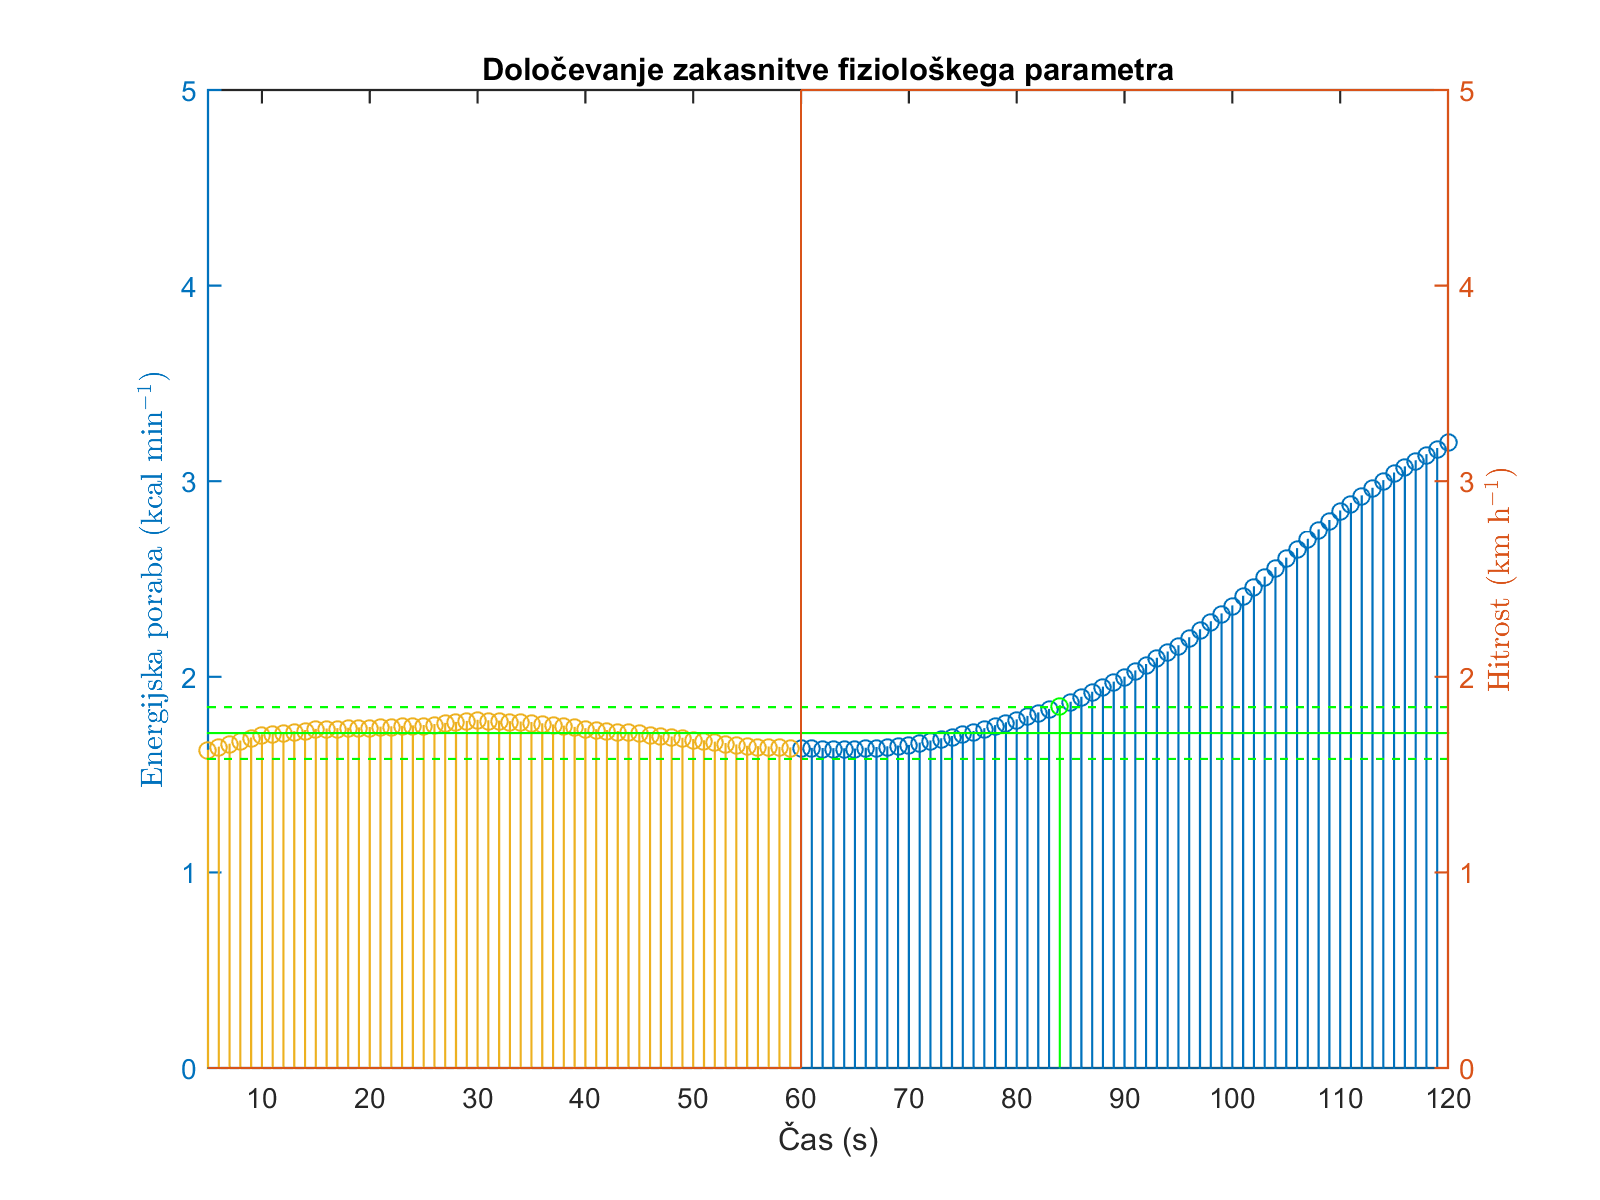
\includegraphics[width=\columnwidth]{./Slike/lag-estimation-1-eem.png}
\caption{Zakasnitev za subjekt 1.}
\label{fig:lag-estimation-train-eem}
\end{subfigure}
~
\begin{subfigure}[t]{0.45\columnwidth}
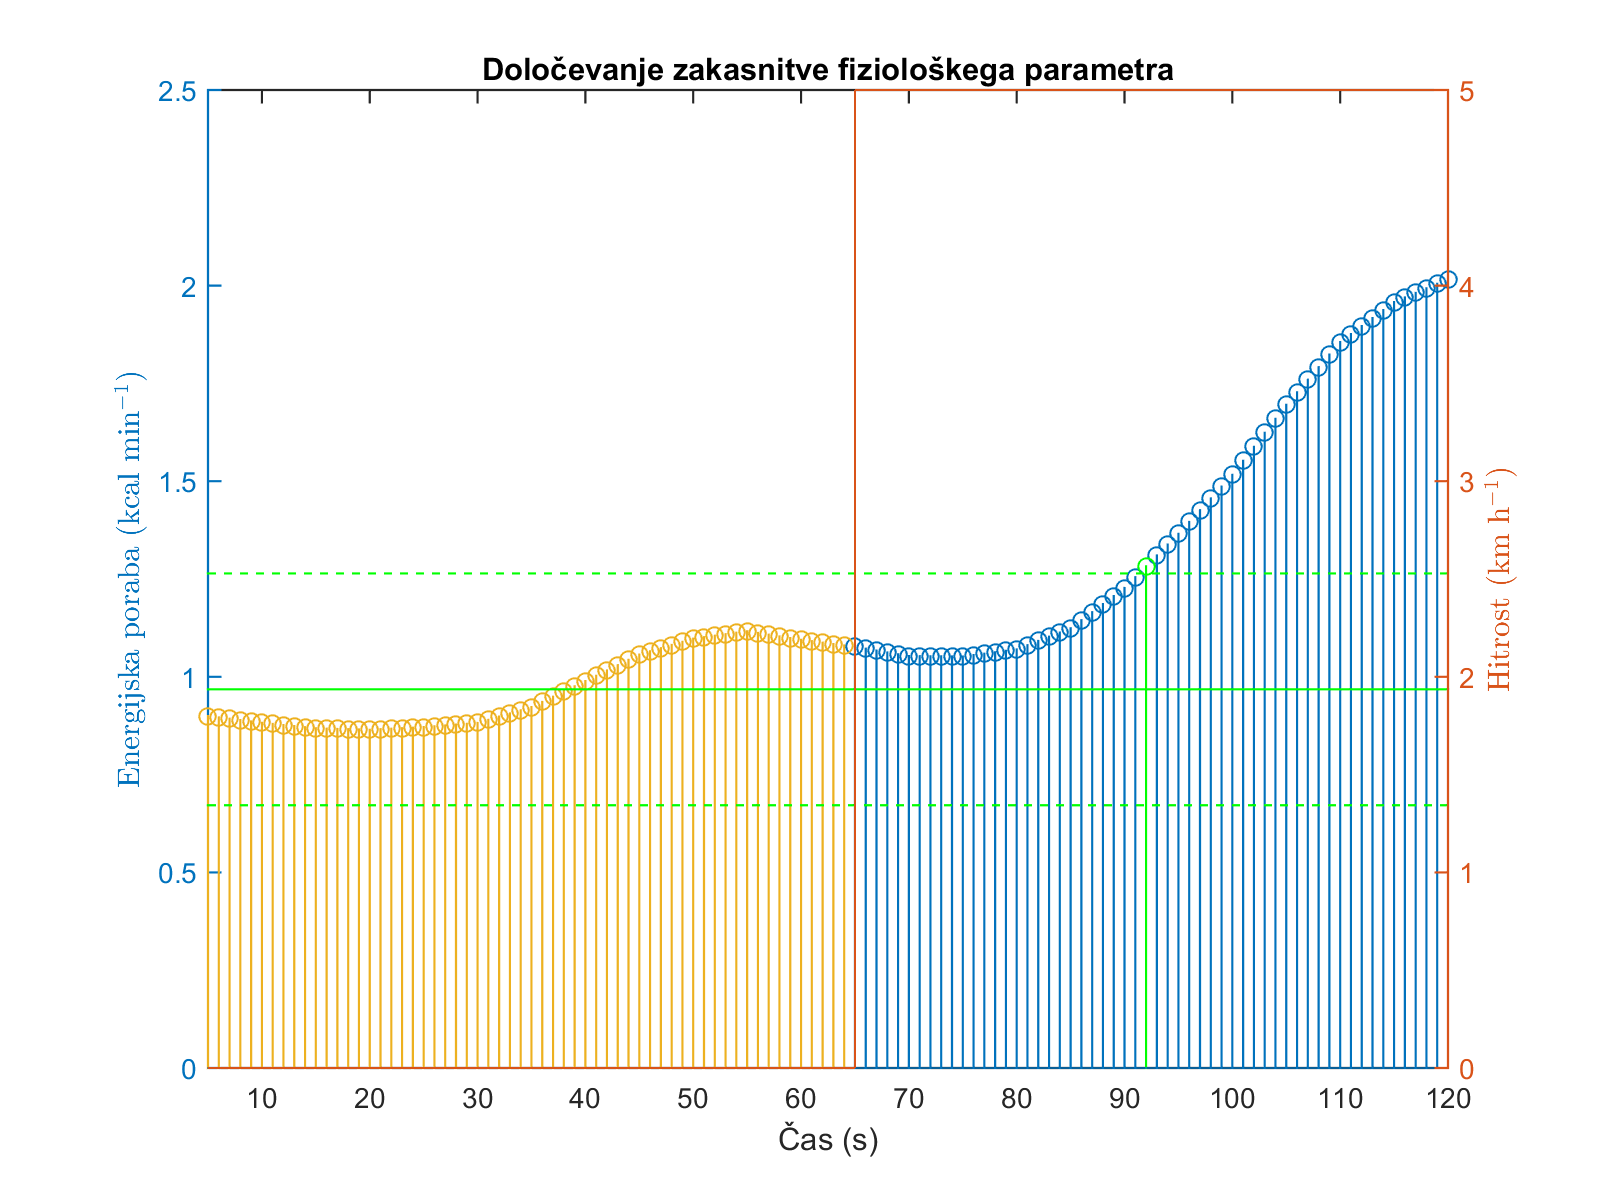
\includegraphics[width=\columnwidth]{./Slike/lag-estimation-2-eem.png}
\caption{Zakasnitev za subjekt 2.}
\label{fig:lag-estimation-train-hr}
\end{subfigure}
~
\begin{subfigure}[t]{0.45\columnwidth}
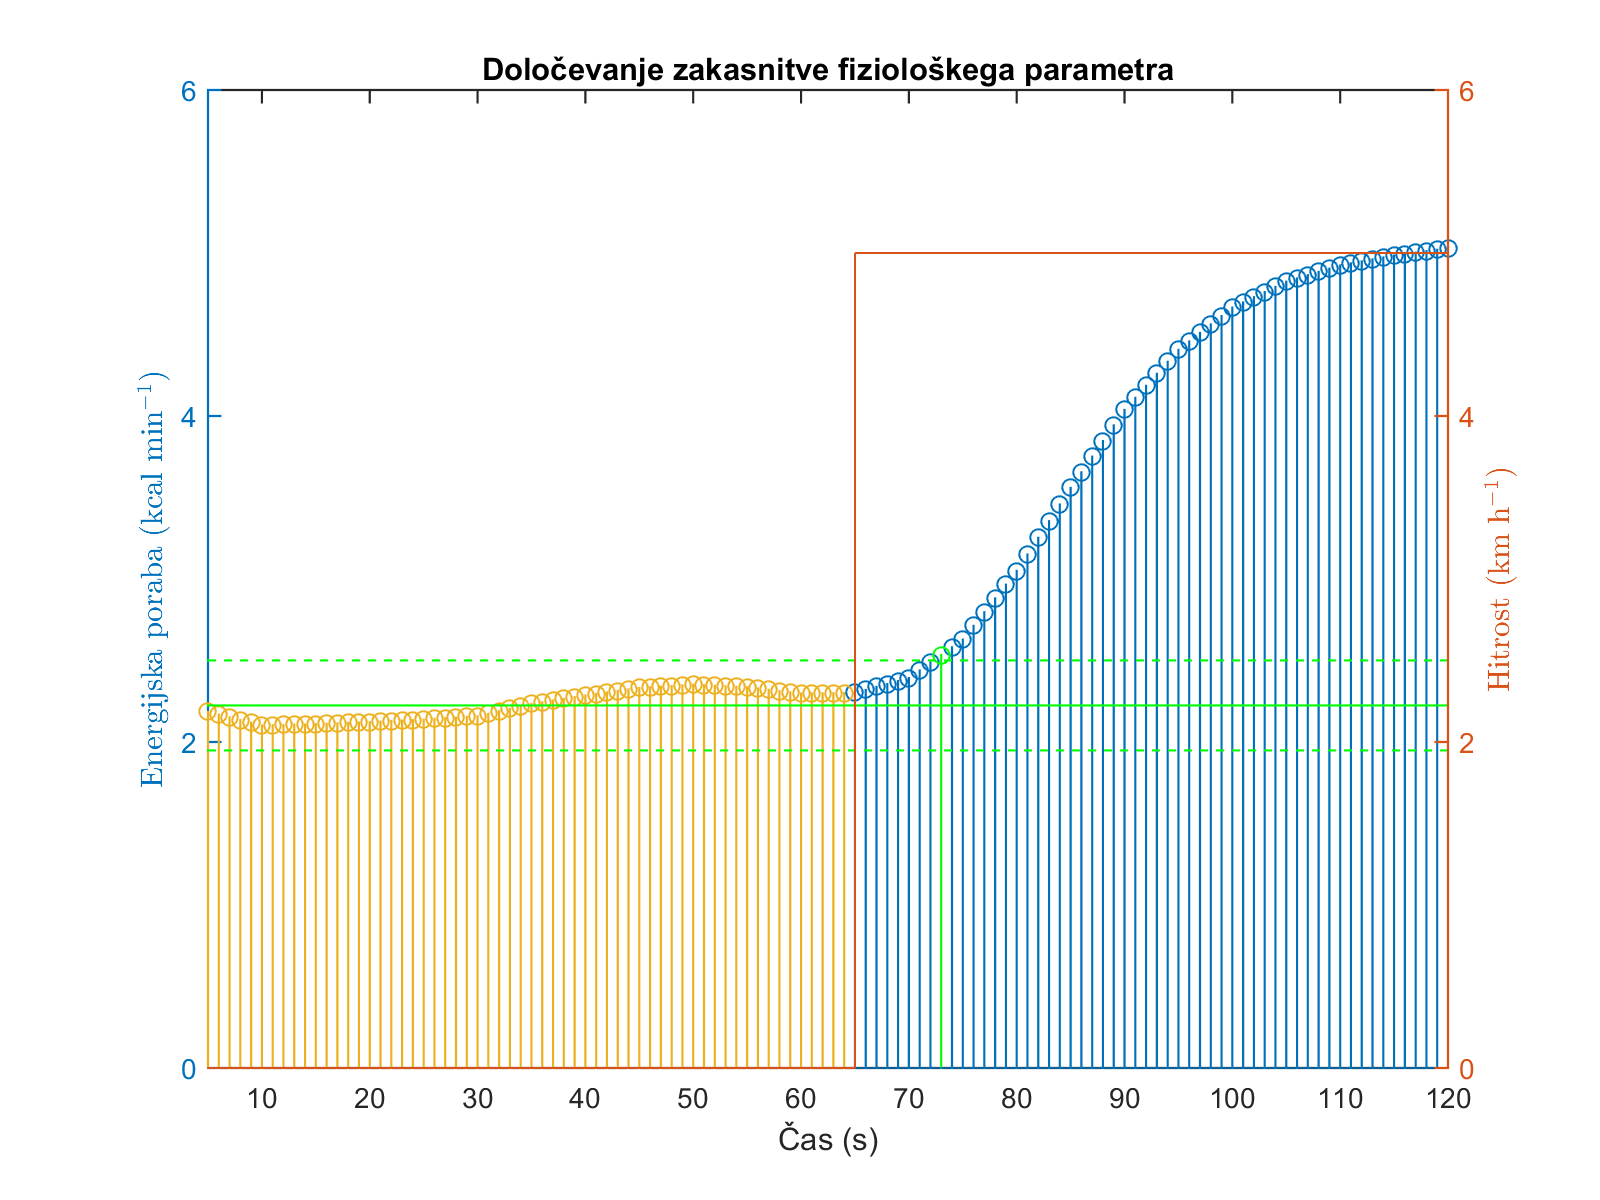
\includegraphics[width=\columnwidth]{./Slike/lag-estimation-3-eem.png}
\caption{Zakasnitev za subjekt 3.}
\label{fig:lag-estimation-train-eem}
\end{subfigure}
~
\begin{subfigure}[t]{0.45\columnwidth}
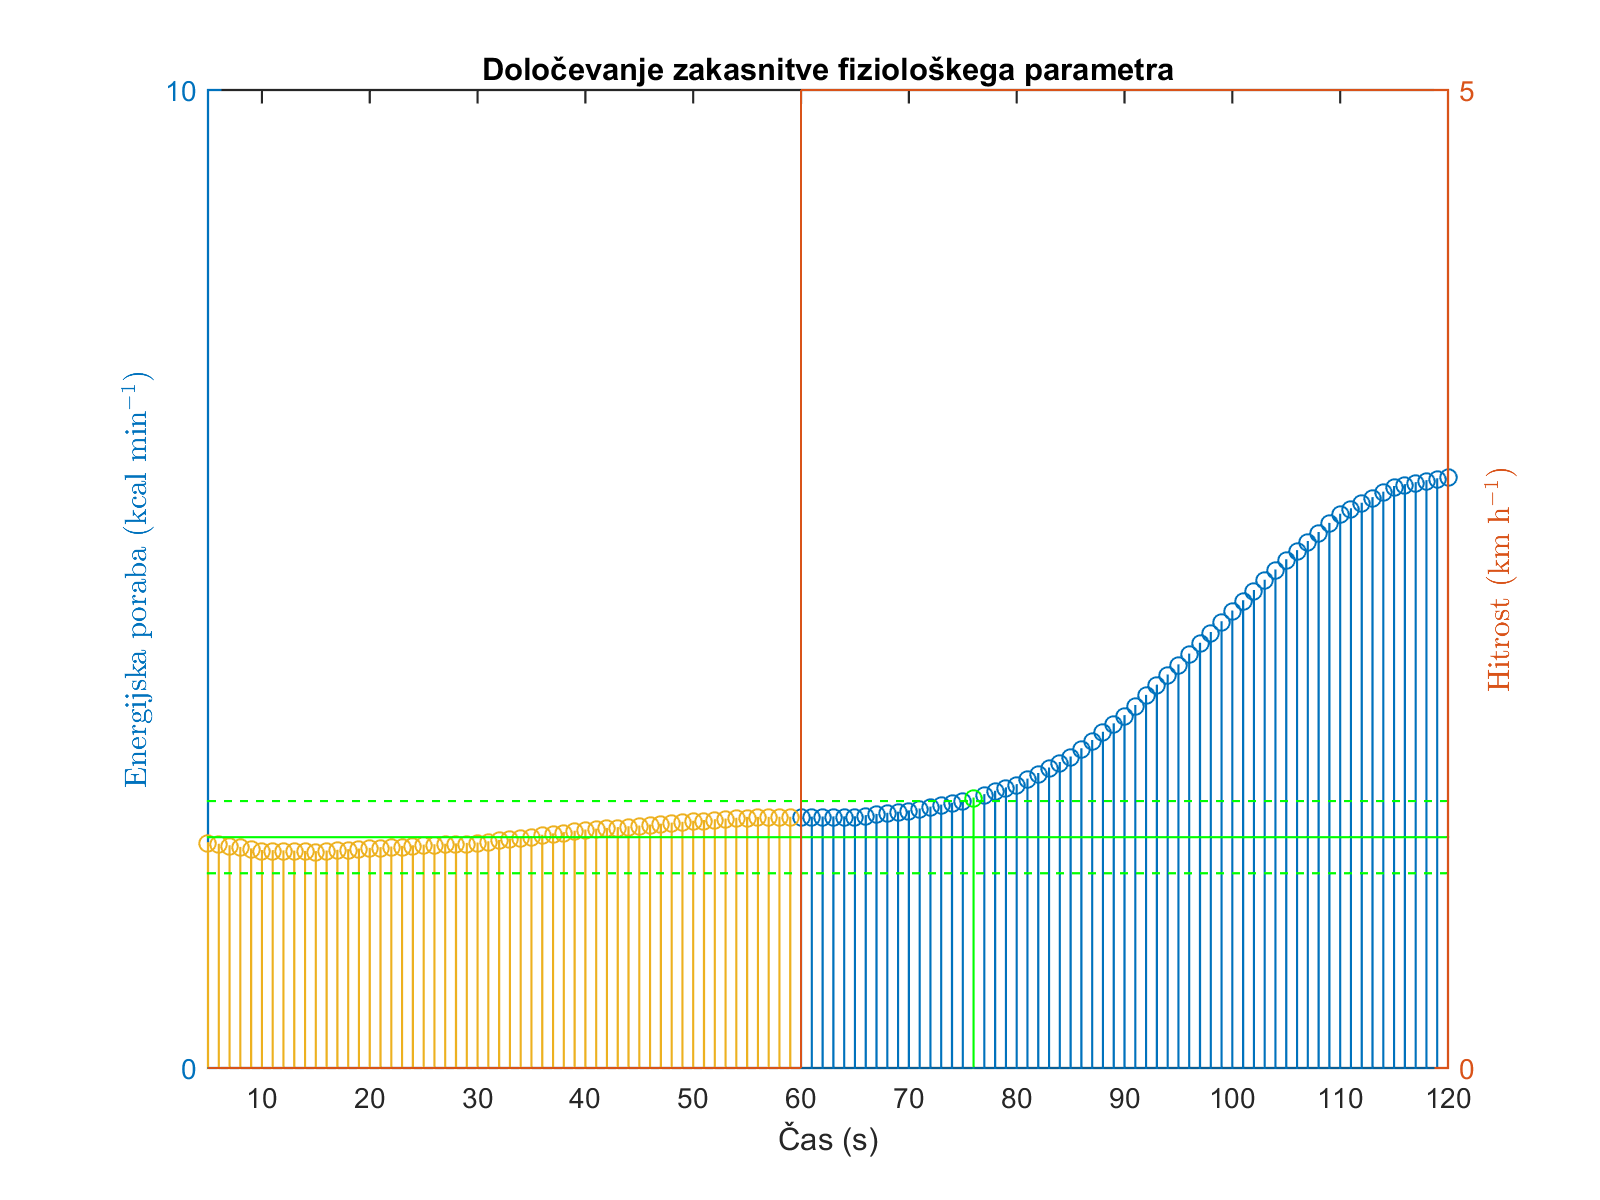
\includegraphics[width=\columnwidth]{./Slike/lag-estimation-4-eem.png}
\caption{Zakasnitev za subjekt 4.}
\label{fig:lag-estimation-train-eem}
\end{subfigure}
~
\begin{subfigure}[t]{0.45\columnwidth}
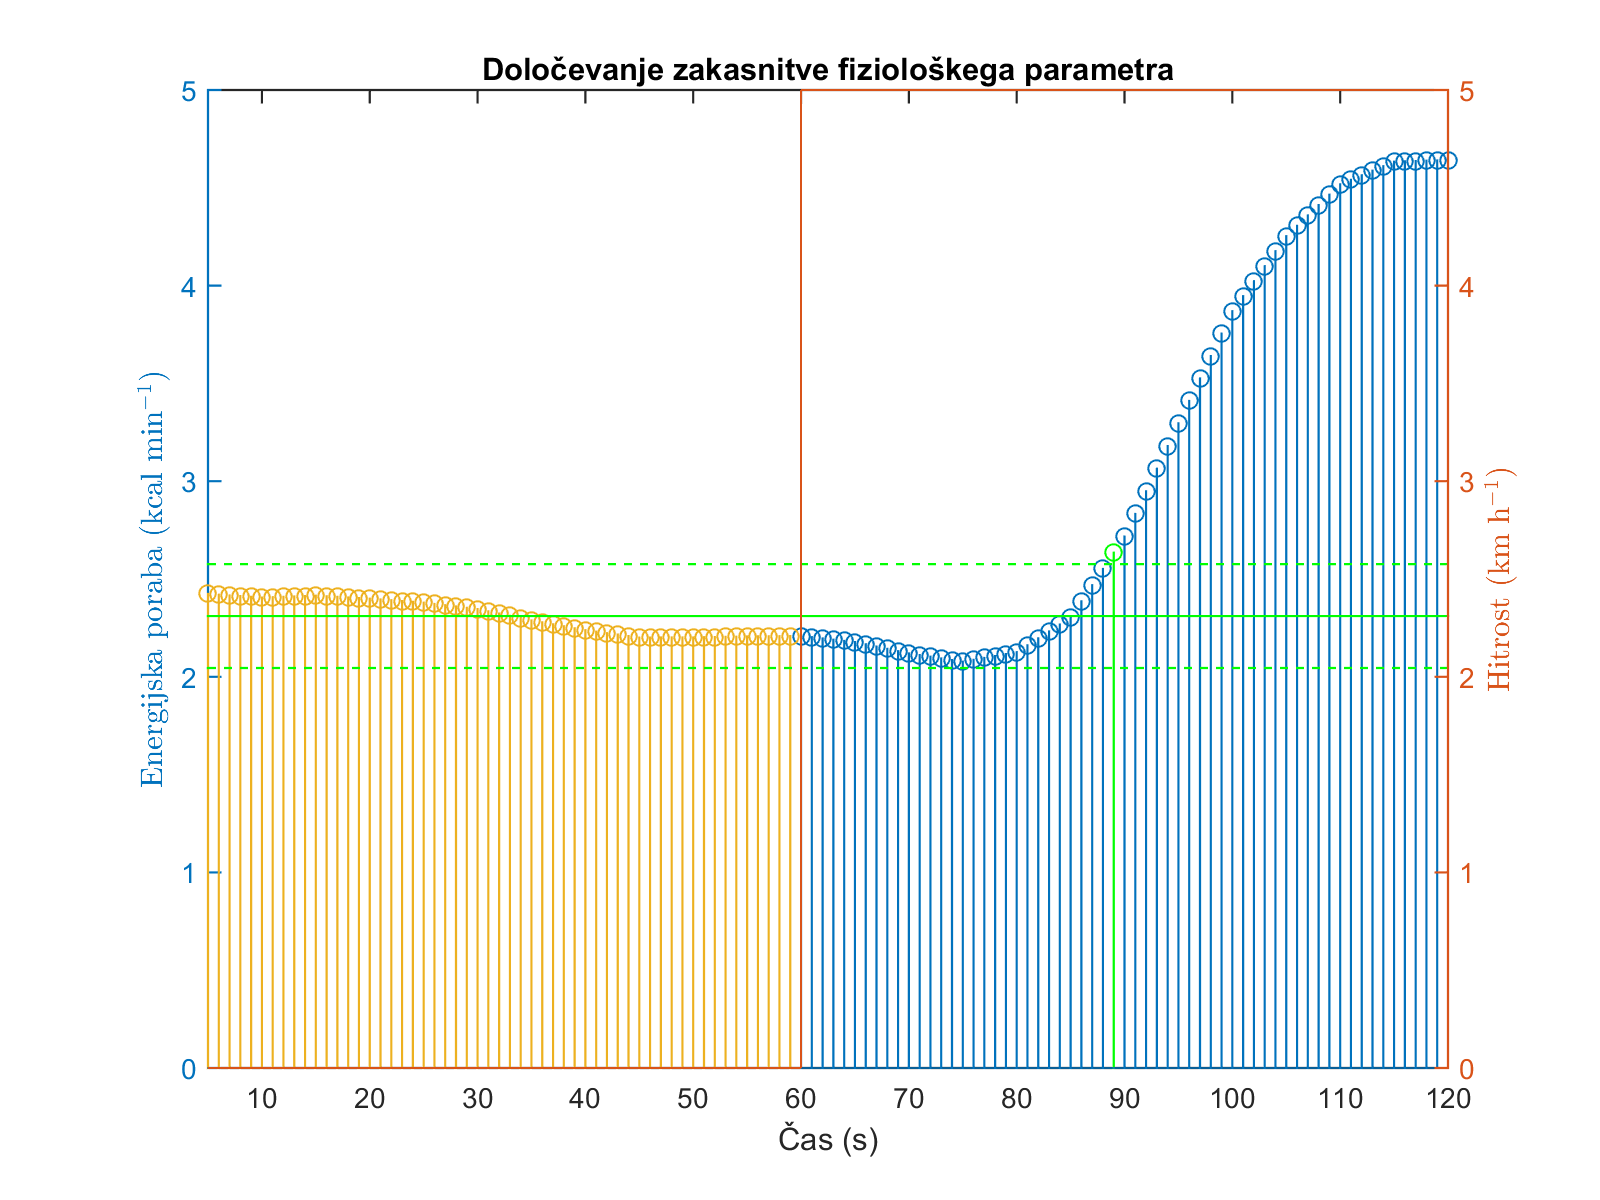
\includegraphics[width=\columnwidth]{./Slike/lag-estimation-5-eem.png}
\caption{Zakasnitev za subjekt 5.}
\label{fig:lag-estimation-train-eem}
\end{subfigure}
~
\begin{subfigure}[t]{0.45\columnwidth}
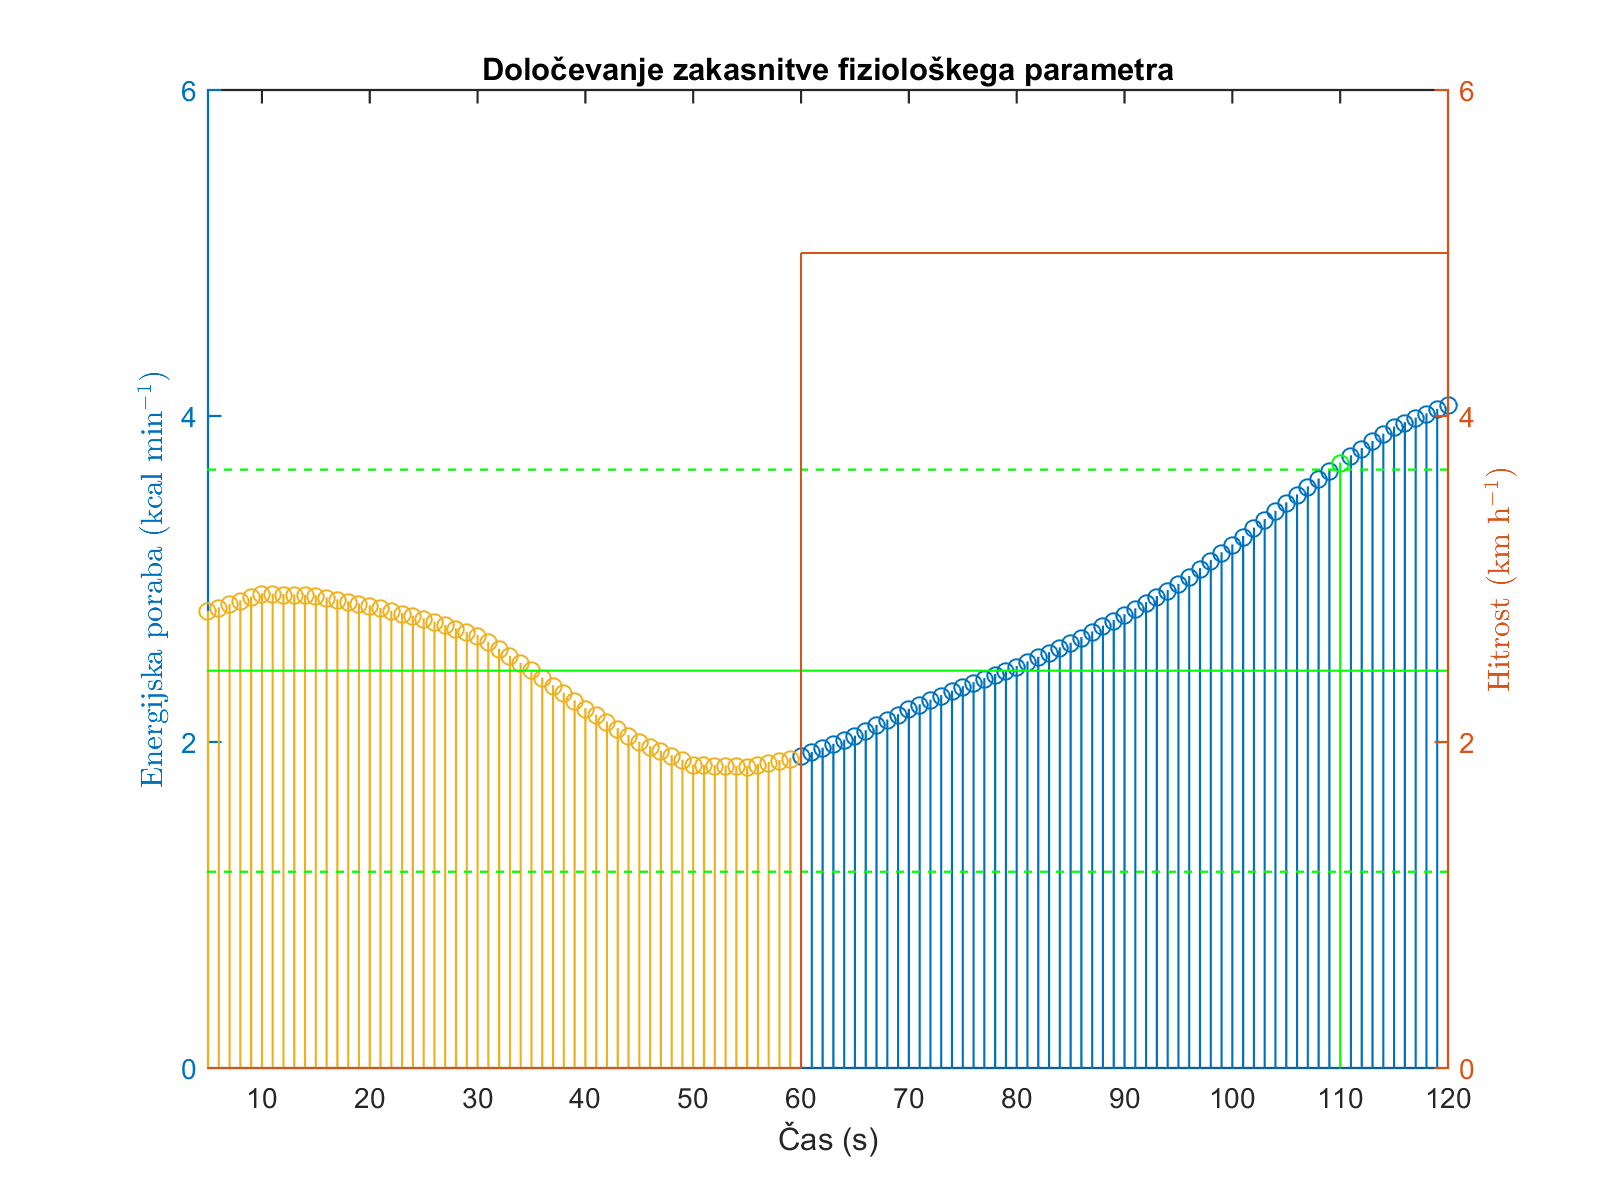
\includegraphics[width=\columnwidth]{./Slike/lag-estimation-6-eem.png}
\caption{Zakasnitev za subjekt 6.}
\label{fig:lag-estimation-train-eem}
\end{subfigure}
\caption{}
\label{fig:lag-estimation-stage1}
\end{figure}



\subsection{Optimizacija Gaussovega filtra}
Pri optimizaciji Gaussovega filtra smo določili optimalni standardni odklon $\sigma$ z uporabo dveh metrik, in sicer: koren srednje kvadratične napake (RMSE) in razmerje med signalom in šumom (SNR). Pri RMSE metriki smo določili napako med učnimi vzorci in njihovo predikcijo. Pri SNR metriki smo za signal uporabili referenčne učne vzorce. Za šum smo uporabili rezidualni ali preostali šum. Tega smo dobili z odštevanjem filtriranih vzorcev od referenčnih. SNR metrika tako določa uspešnost izločevanja šuma, RMSE metrika pa pravilnost določevanja kateri podatki spadajo v signal in kateri v šum.


Teste smo izvajali na vseh eksperimentih 1. sklopa, pri čemer smo uporabili $\nu$-RBF jedro s \SI{50}{\%} podpornih vektorjev. Za filtriranje pri mrežnem iskanju smo izbrali najmanjši filter s $\sigma = 1$. Testirali smo naslednje standardne odklone Gaussovega filtra: $1, 3, 5, 11, 21, 31$ in $51$. 

Rezultati povrprečnih vrednosti uporabljenih metrik so vidni v tabeli \ref{tab:gauss}. Za pravilno razlago rezultatov, moramo upoštevati tudi grafe metrik posameznih eksperimentov, ki so prikazani na slikah \ref{fig:sigma1-5}, \ref{fig:sigma-rmse5-21} in \ref{fig:sigma21-51}. 



\begin{table}[htb]
	\centering
    \begin{tabular}{S[table-format=2.0] S[table-format=2.3] S[table-format=2.3]}
    \toprule
    \thead{$\mathbf{\sigma}$} & \thead{RMSE} & \thead{SNR [dB]}  \\
    \midrule%nSV
    1 & \boldentry{2.3}{8.614} & 24.278 \\
    3 & 11.236 & 25.470 \\
    \boldentry{2.0}{5} & 11.596 & 25.746 \\
    11 & 11.783 & 25.746 \\
    21 & 11.842 & 25.975 \\
    31 & 11.871 & 26.194 \\
    51 & 11.907 & \boldentry{2.3}{26.306} \\
    \bottomrule
    \end{tabular}
    \caption[Povprečne vrednosti RMSE in SNR metrik pri optimizaciji parametra $\sigma$ Gaussovega filtra]{Povprečne vrednosti RMSE in SNR metrik pri optimizaciji parametra $\sigma$ Gaussovega filtra. Najmanjši standardni odklon ima najmanjšo napako, vendar je tudi filtriranje majhno. Pri $\sigma=3$ in $\sigma=5$ so še opazne razlike pri filriranju. Za višje vrednosti ni več opazne razlike, vendar pa se napaka povečuje. $\sigma=5$ je tako optimalna vrednosti parametra.}
    \label{tab:gauss}
\end{table}

Najmanjšo napako dobimo, če uporabimo $\sigma=1$, vendar pa imamo pri tem najmanjše filtriranje, zato so rezultati še vedno lahko zelo šumni. Z višanjem parametra filtra, se napaka po metriki RMSE povečuje, vendar ima večji vpliv razmerje SNR, saj je predstavljeno v logaritemski skali. 

\begin{figure}[htb]
\centering
\begin{subfigure}[t]{0.45\columnwidth}
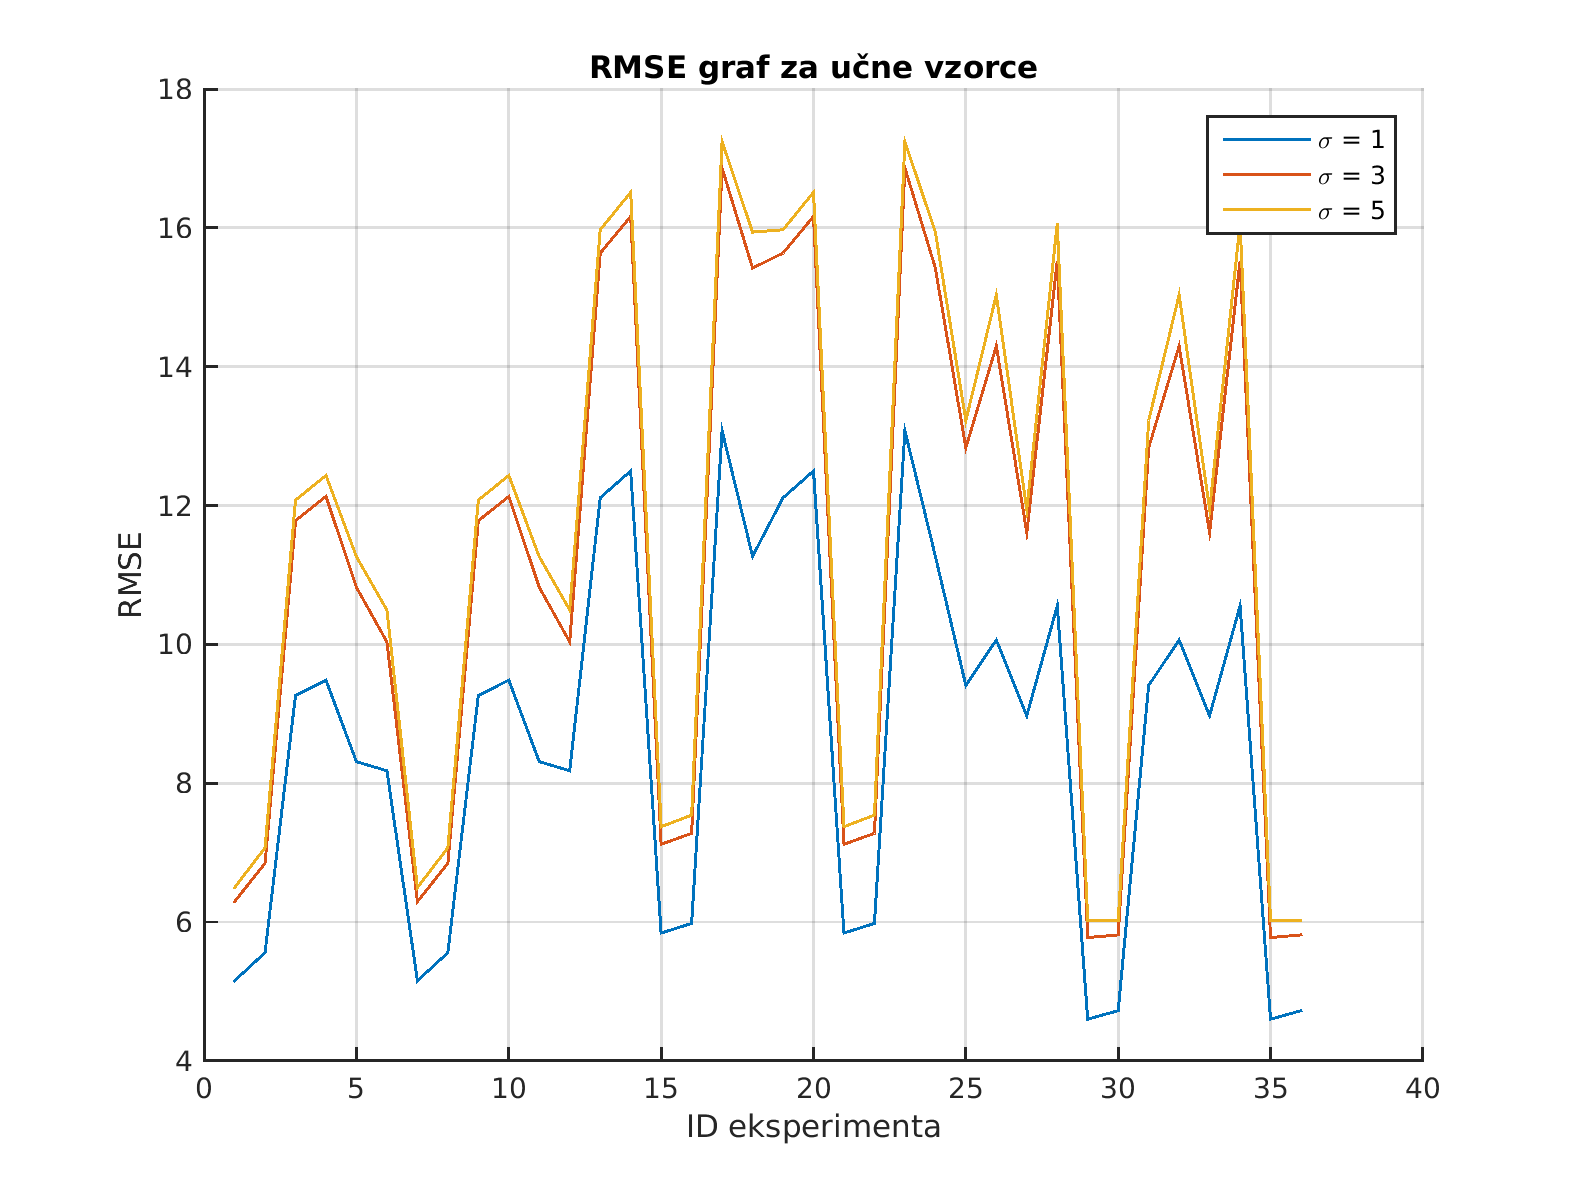
\includegraphics[width=\columnwidth]{./Slike/sigma-rmse1-5.png}
\caption{Graf RMSE  učnih vzorcev }
\label{fig:sigma-rmse1-5}
\end{subfigure}
~
\begin{subfigure}[t]{0.45\columnwidth}
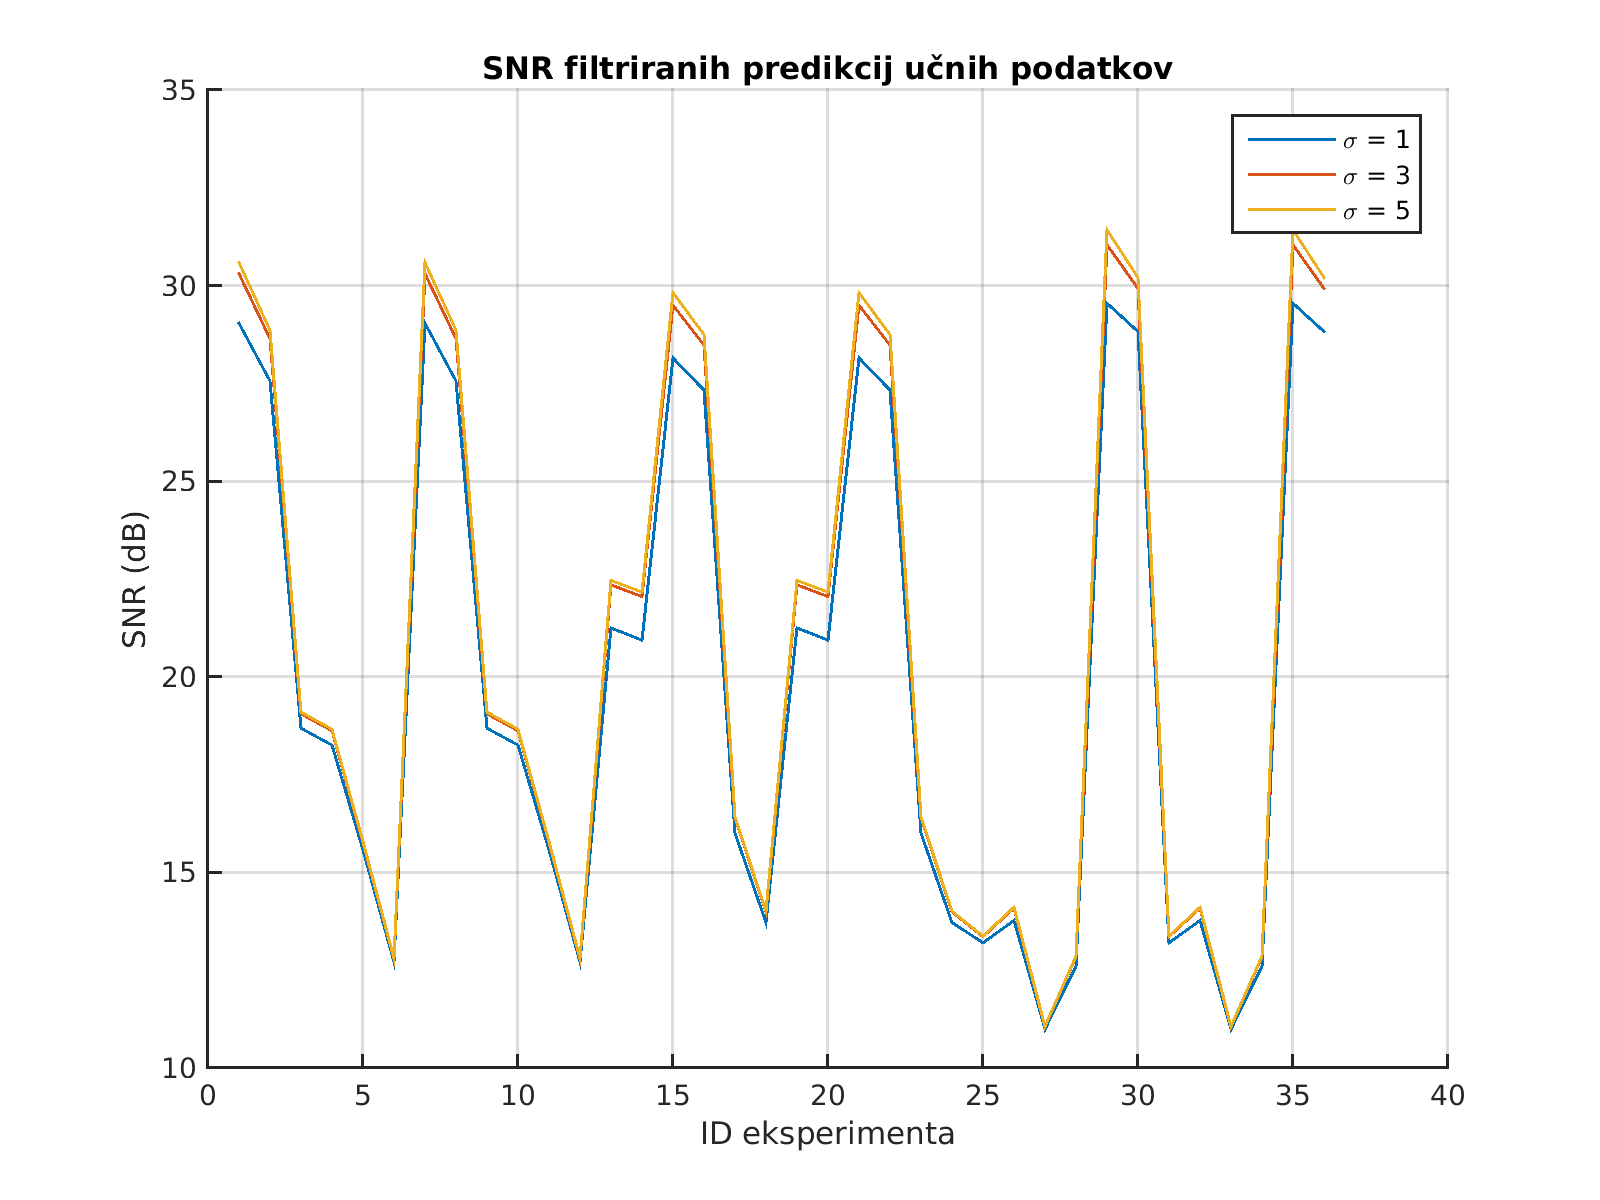
\includegraphics[width=\columnwidth]{./Slike/sigma-snr1-5.png}
\caption{Graf SNR  učnih vzorcev}
\label{fig:sigma-snr1-5}
\end{subfigure}
\caption{Grafa RMSE in SNR učnih vzorcev za \mbox{$\sigma \in [1,5]$}}
\label{fig:sigma1-5}
\end{figure}

Čeprav pri uporabi $\sigma=51$ dobimo največje filtriranje šuma, lahko na slikah grafov opazimo, da se obe metriki bistveno ne razlikujeta za vrednosti parametra na intervalu $[5,51]$. Kljub dobremu filtriranju želimo zagotoviti čim manjšo napako med referenčnim signalom in predikcijo, zato je logična izbira čim manjši standardni odklon. Ker so na sliki \ref{fig:sigma1-5} med $\sigma=3$ in $\sigma=5$ še opazne razlike, lahko zaključimo, da je $\sigma=5$ optimalna izbira parametra za naš problem. 


\begin{figure}[htb]
\centering
\begin{subfigure}[t]{0.45\columnwidth}
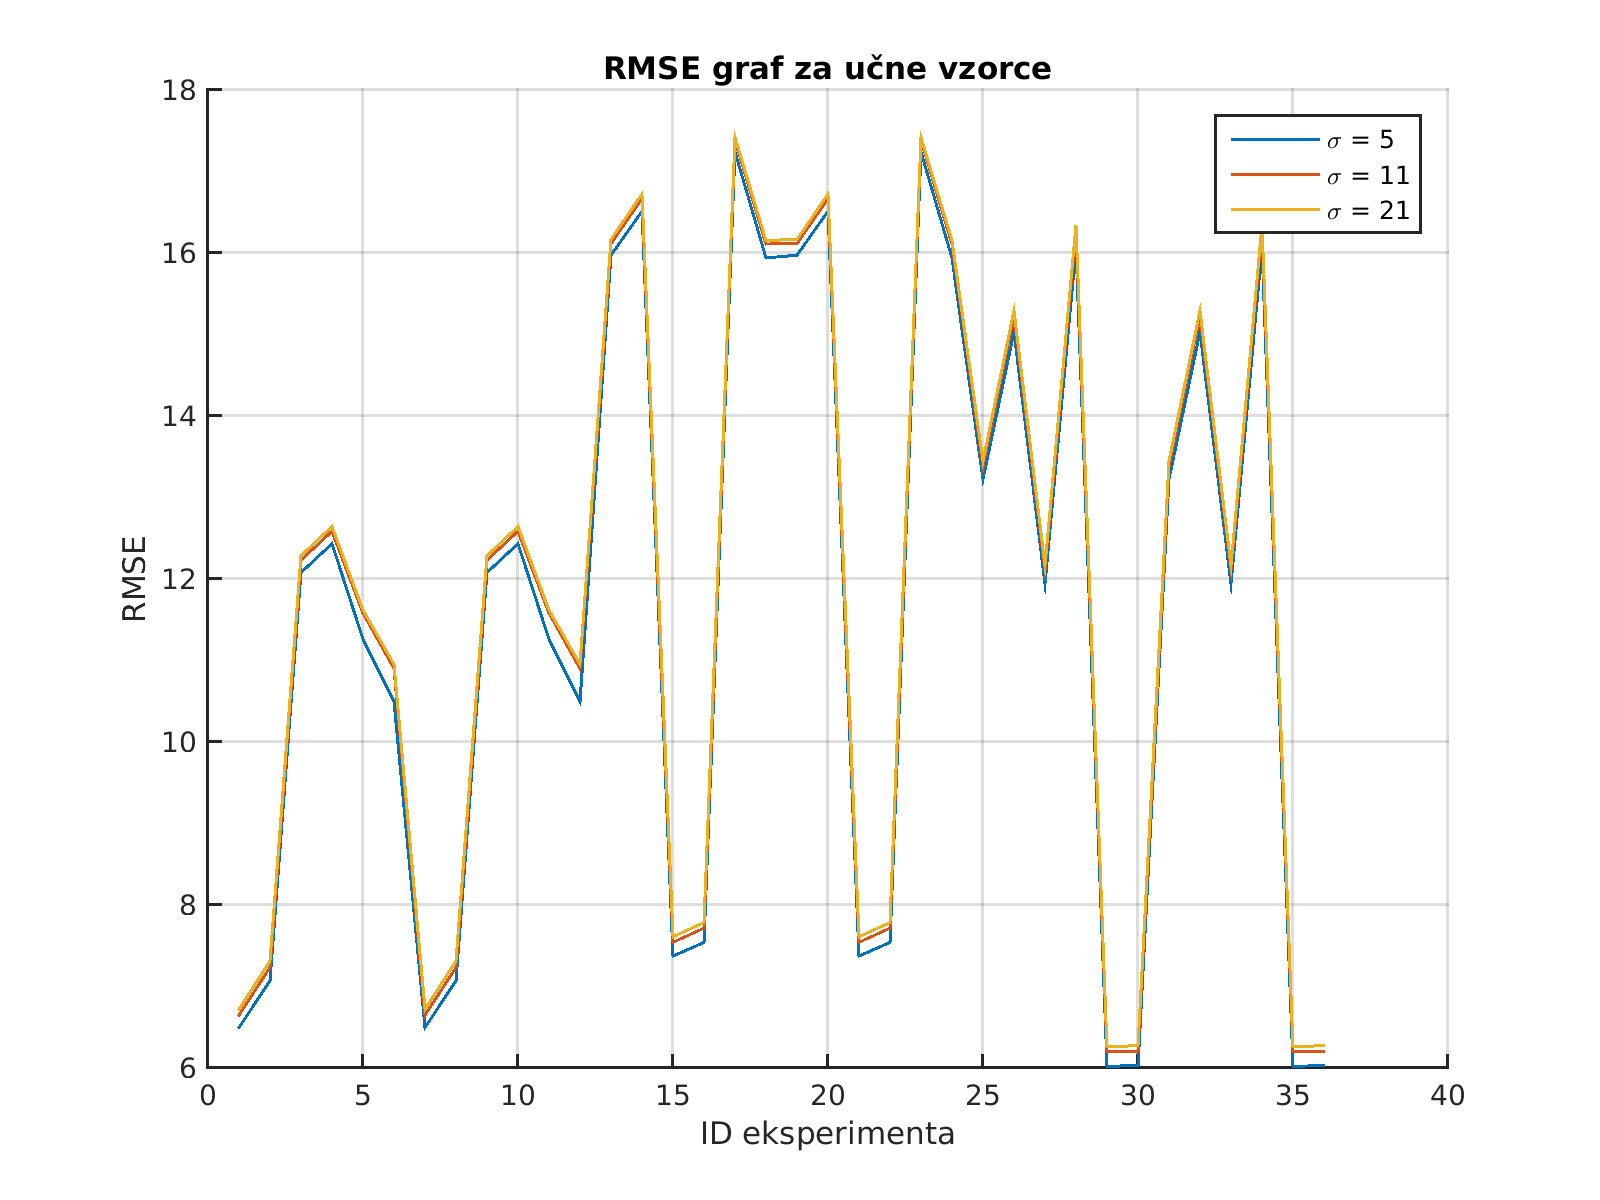
\includegraphics[width=\columnwidth]{./Slike/sigma-rmse5-21.png}
\caption{Graf RMSE  učnih vzorcev}
\label{fig:sigma-rmse5-21}
\end{subfigure}
~
\begin{subfigure}[t]{0.45\columnwidth}
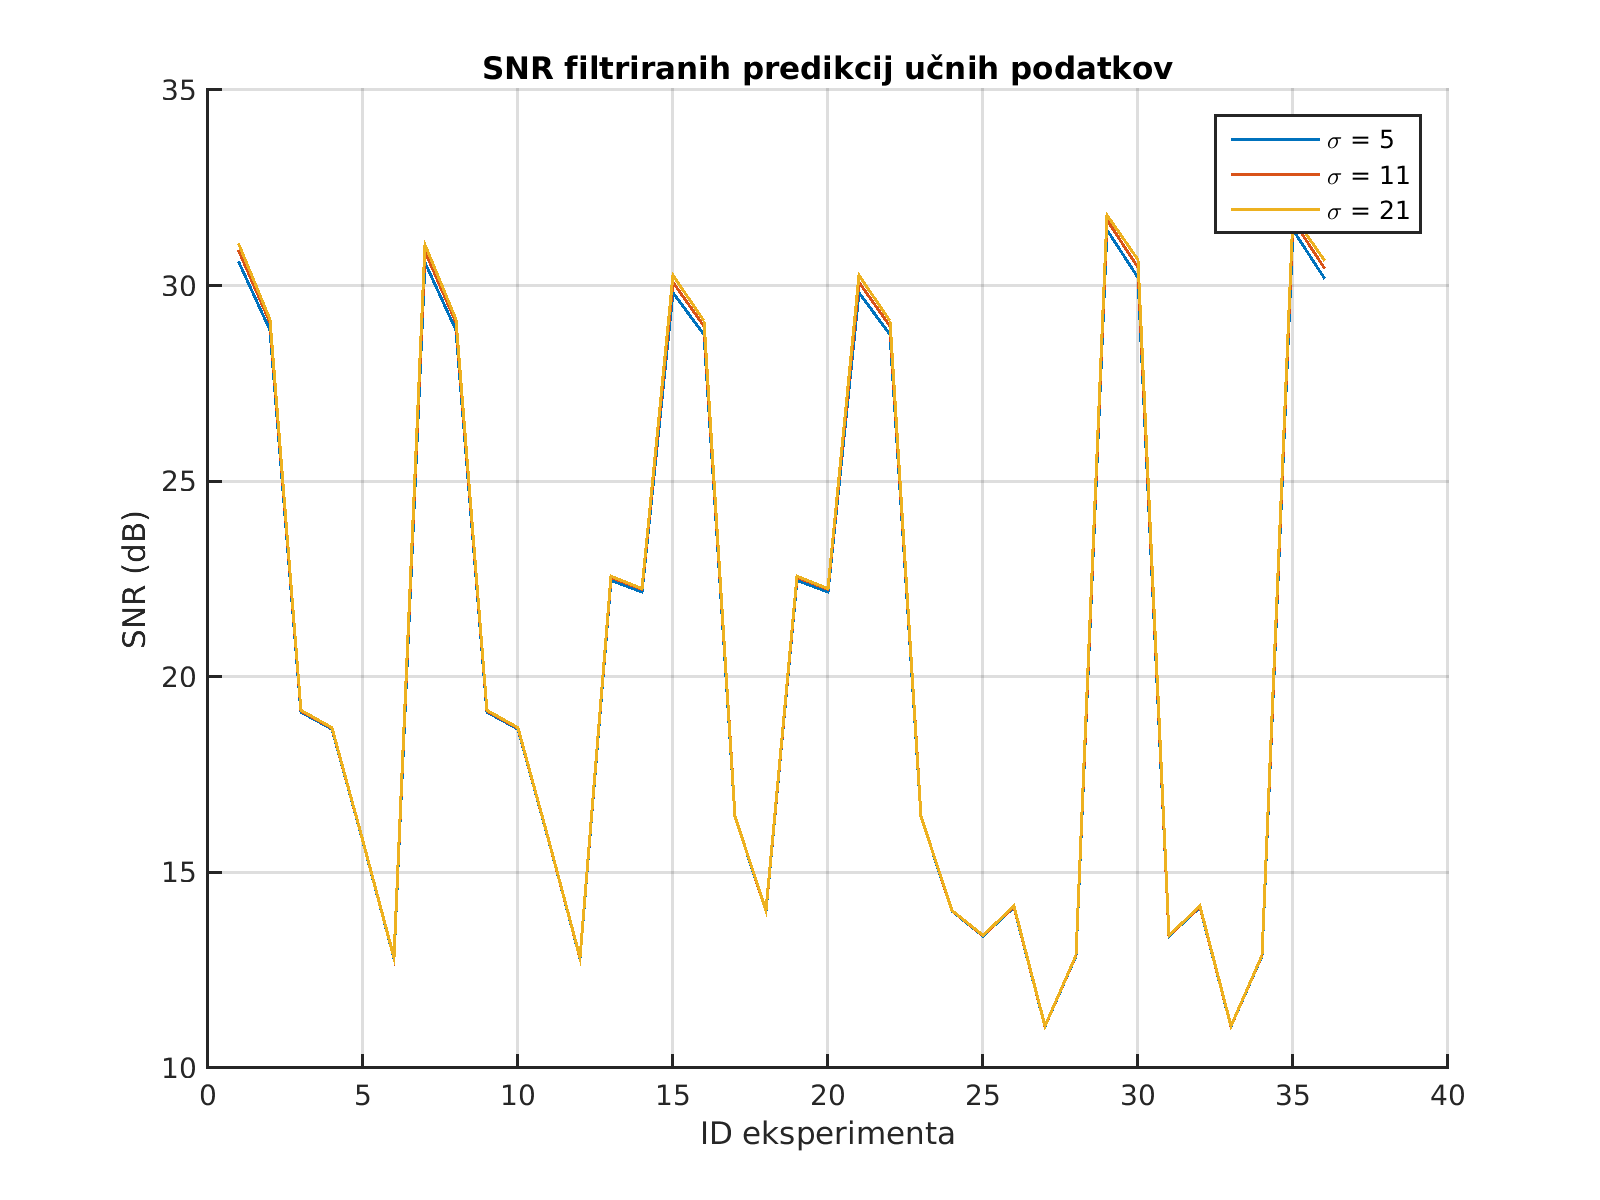
\includegraphics[width=\columnwidth]{./Slike/sigma-snr5-21.png}
\caption{Graf SNR  učnih vzorcev}
\label{fig:sigma-snr5-21}
\end{subfigure}
\caption{Grafa RMSE in SNR učnih vzorcev za \mbox{$\sigma \in [5,21]$}}
\label{fig:sigma5-21}
\end{figure}



\begin{figure}[htb]
\centering
\begin{subfigure}[t]{0.45\columnwidth}
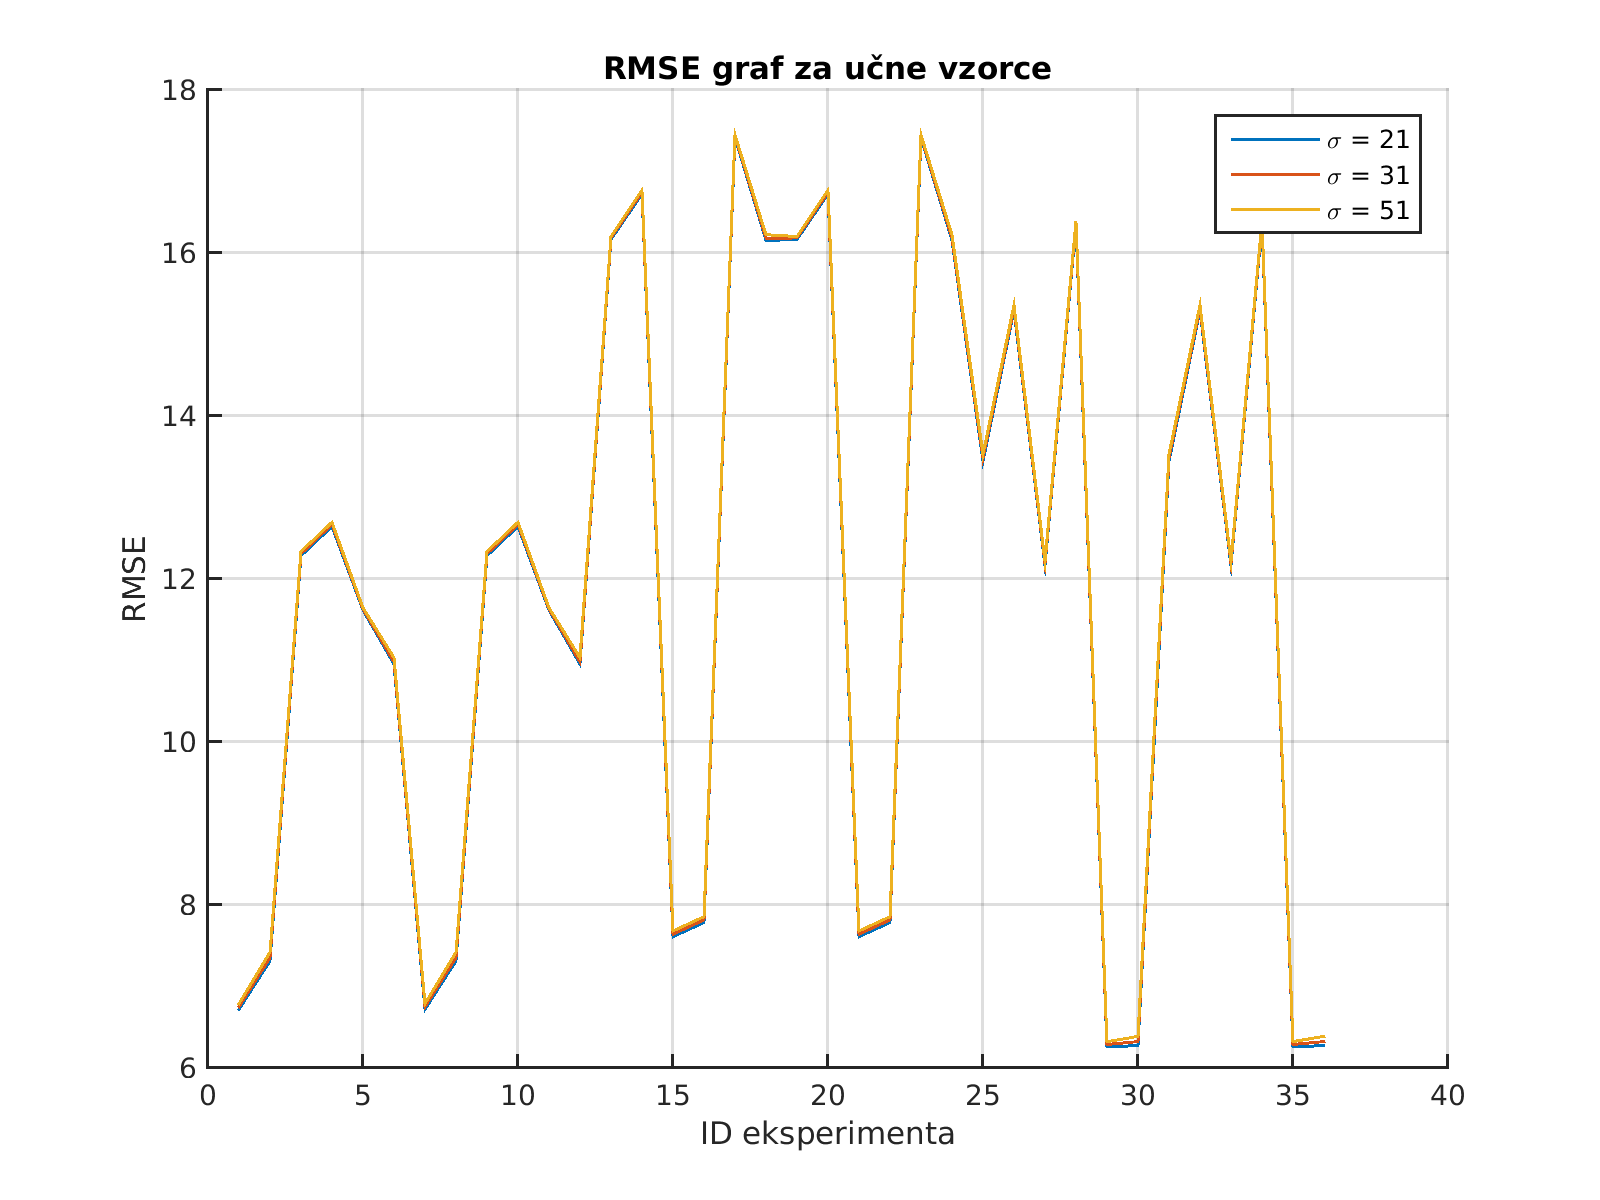
\includegraphics[width=\columnwidth]{./Slike/sigma-rmse21-51.png}
\caption{Graf RMSE učnih vzorcev}
\label{fig:sigma-rmse21-51}
\end{subfigure}
~
\begin{subfigure}[t]{0.45\columnwidth}
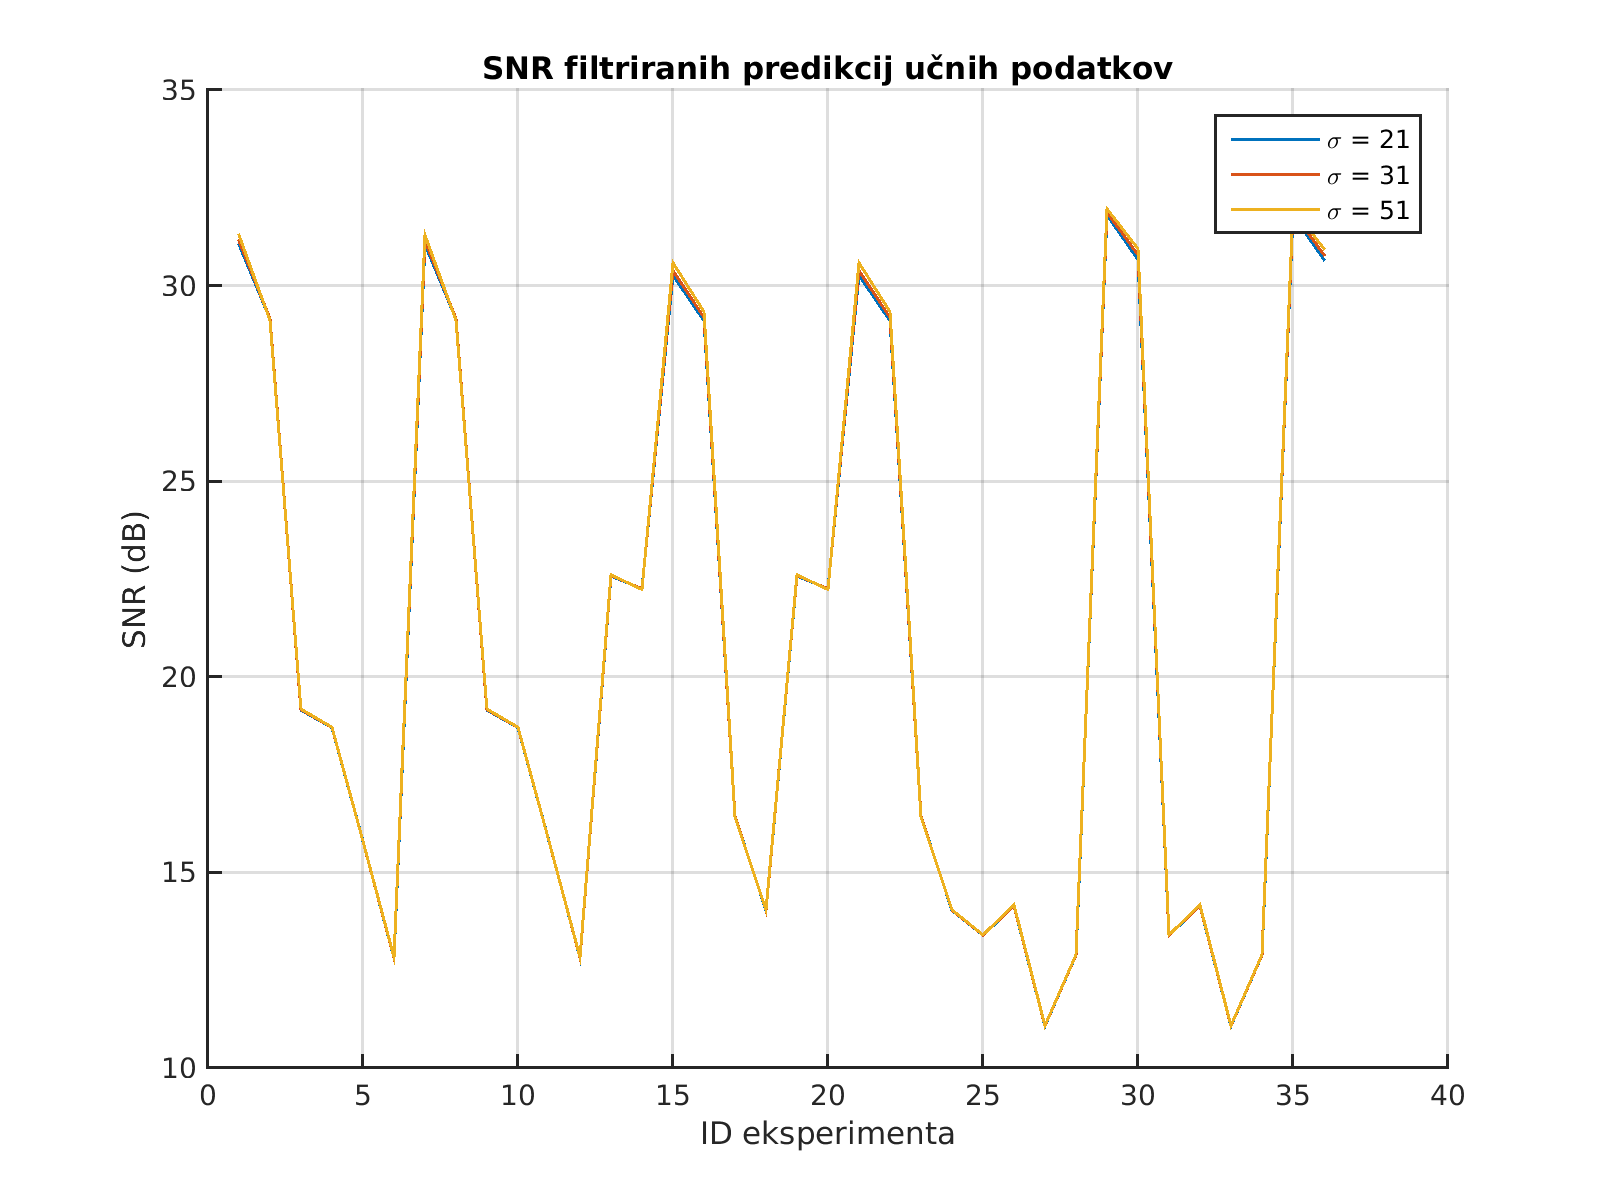
\includegraphics[width=\columnwidth]{./Slike/sigma-snr21-51.png}
\caption{Graf SNR  učnih vzorcev}
\label{fig:sigma-snr21-51}
\end{subfigure}
\caption{Grafa RMSE in SNR učnih vzorcev za \mbox{$\sigma \in [21,51]$}}
\label{fig:sigma21-51}
\end{figure}


\subsubsection{Regresija \texorpdfstring{$\nu$}{nu}-RBF}



\subsection{Laboratorijski eksperimenti}
a

\subsection{Terenski eksperimenti}
a

\section{Rezultati}
All energy consumption and heart rate models were validated on previously described test samples. For comparison between the different models we have chosen validation measures: correlation coefficient (CORR), relative absolute error (RAE) and root relative square error (RRSE) \cite{witten2005data}.The higher the value of the CORR the better, with RAE and RRSE is other way around.

% Dodati moram da sem 8 initial modelov potem cross teste delal
Models were also evaluated with cross testing. This testing was done only by the type of input data---side-view or back-view. \textit{sv} models, that were made with learning samples from side-view camera were first tested with testing samples from side-view camera and then with back-view camera. Hereafter tests with input data from side-view camera are marked with \textit{sv} in brackets and tests with input data from back-view camera are marked with \textit{bv} in brackets.

\subsection{Treadmill results}\label{sec:initial-models}
As can be seen in the Table \ref{tab:initial-models-validation}, we get relatively poor results in the prediction of heart rate.

\begin{table}[!htb]
	\centering
	{\footnotesize
      \begin{tabular}{l S[table-format=3.2, detect-weight, detect-shape, detect-mode] S[table-format=3.2, detect-weight, detect-shape, detect-mode] S[table-format=3.2, detect-weight, detect-shape, detect-mode]}
          \toprule
          \textbf{Model} & \multicolumn{1}{c}{\textbf{CORR}} & \multicolumn{1}{c}	{\textbf{RAE} (\%)} & \multicolumn{1}{c}{\textbf{RRSE} (\%)} \\
          \midrule
          hr-sv(sv) & 0.90 & 75.42 & 76.66	\\
          hr-sv(bv)	&	-0.66	&	104.61	&	110.17	\\
\bfseries hr-sv-lag(sv)		&	\bfseries 0.93	&	\bfseries 74.37	&	\bfseries 75.51	\\
          hr-sv-lag(bv)	&	-0.87	&	138.60	&	136.62	\\
          hr-bv(sv)	&	0.83	&	311.95	&	295.66	\\
          hr-bv(bv)	 	&	0.88	&	81.07	&	79.27	\\
          hr-bv-lag(sv)	&	0.49	&	84.71	&	89.40	\\
          hr-bv-lag(bv) 	&	0.91	&	79.15	&	76.93	\\
          eem-sv(sv)		&	0.87	&	47.08	&	49.75	\\
          eem-sv(bv)	&	-0.75	&	109.27	&	117.62	\\
          \bfseries eem-sv-lag(sv)	&	\bfseries 0.92	&	\bfseries 38.15	&	\bfseries 40.18	\\
          eem-sv-lag(bv)	&	-0.74	&	121.86	&	121.88	\\
          eem-bv(sv)	&	0.61	&	94.92	&	95.92	\\
          eem-bv(bv)		&	0.85	&	44.51	&	56.24	\\
          eem-bv-lag(sv)	&	0.86	&	56.60	&	68.61	\\
          eem-bv-lag(bv)	&	0.90	&	45.51	&	49.50	\\
          \bottomrule        
      \end{tabular}
	}
	\caption{The results of the initial model evaluations with cross testing. For each model, we calculated the correlation coefficient (CORR), relative absolute error (RAE) and root relative square error (RRSE).}
	\label{tab:initial-models-validation}
\end{table}

In terms of using different view angles, we get best results for side-view. We assume that this is due to the fact that with a back-view camera (without any cropping) we also recorded the movement of the operator, who is not visible in side-view recordings. Despite the fact that the HOOF features get rid of the noise of the optical flow, the movement of the operator is intensive enough to be able to influence the results. Worse results for back-view camera could also indicate that we get less descriptive features from it. 
%V smislu uporabe različnih zornih kotov, smo dobili najboljše rezultate pri stranskem pogledu. Predvidevamo, da je to posledica dejstva, da smo s kamero pri hrbtnem pogledu snemali tudi gibanje operaterja, česar pa v stranskem pogledu ni. Kljub dejstvu, da se s HOOF značilkami znebimo šuma optičnega toka, je gibanje operaterja dovolj intenzivno, da bi lahko vplivalo na rezultat.

The results of the models, where we assume the delay between excitation and response are better, which indicates that the assumption is justified.
%Rezultati modelov, kjer smo predpostavili časovni zamik med vzbujanjem in odzivom so boljši, kar nakazuje na to, da je predpostavka upravičena.

Considering cross testing we can see, that all models produce poorer results if we test them with data from different viewing angle.

The best results were obtained in the prediction of the energy expenditure (EEM). Output signals of the best results for the prediction of energy expenditure and heart rate are presented in Figure \ref{fig:rezultat}. The curves of the results have the same form because they are correlated physiological parameters.
%Najboljši rezultat smo dobili pri predikciji hitrosti porabe energije (EEm). Izhodni signali najboljših rezultatov za predikcijo energijske porabe in srčnega utripa so predstavljeni na sliki \ref{fig:rezultat}.

\begin{figure}[!htb]
	\centering
    %\includegraphics[width=0.9\linewidth]{./slike/best-results.eps}
    \caption{The best results for prediction of energy expenditure and heart rate when validating the models. The figure shows the output of models eem-sv-lag(sv) and hr-sv-lag(sv) and the actual value of energy expenditure and heart rate.}
    %\caption{Najboljša rezultata za predikcijo porabe energije in srčnega utripa pri validaciji modelov. Slika prikazuje izhod modelov eem-sv-l in hr-sv-l ter dejanske vrednosti hitrosti porabe energije na minuto in srčnega utripa.}
    \label{fig:rezultat}
\end{figure}

\subsection{Mixed-view experiments}
As in \ref{sec:initial-models}, when comparing models with different physiological parameters in Table \ref{tab:mixed-models-validation}, heart rate models produce worse results. Lag models are better than normal models and best result is still produced by lagged model, which predicts energy expenditure.

\begin{table}[!htb]
	\centering
	{\footnotesize
      \begin{tabular}{l  S[table-format=3.2, detect-weight, detect-shape, detect-mode]  S[table-format=3.2, detect-weight, detect-shape, detect-mode]  S[table-format=3.2, detect-weight, detect-shape, detect-mode]}
          \toprule
          \textbf{Model} & \multicolumn{1}{c}{\textbf{CORR}} & \multicolumn{1}{c}	{\textbf{RAE} (\%)} & \multicolumn{1}{c}{\textbf{RRSE} (\%)} \\
          \midrule
        hr-mixed(sv)	&	0.89	&	67.18	&	68.17	\\
        hr-mixed(bv)	&	0.88	&	59.84	&	61.89	\\
        hr-mixed-lag(sv) &	0.92	&	65.24	&	66.44	\\
        \bfseries hr-mixed-lag(bv) &	\bfseries 0.91	&	\bfseries 57.75	&	\bfseries 60.31	\\
        eem-mixed(sv)	&	0.85	&	45.90	&	53.89	\\
        eem-mixed(bv)	&	0.84	&	57.44	&	62.78	\\
        \bfseries eem-mixed-lag(sv)	&	\bfseries 0.90	&	\bfseries 44.19	&	\bfseries 46.09	\\
        eem-mixed-lag(bv)	&	0.89	&	56.70	&	55.04	\\
          \bottomrule        
      \end{tabular}
	}
	\caption{The results of the mixed model evaluations with cross testing. For each model, we calculated the correlation coefficient (CORR), relative absolute error (RAE) and root relative square error (RRSE).}
	\label{tab:mixed-models-validation}
\end{table}

The main difference in mixed models can be seen, when comparing cross tests. If we compare results from Table \ref{tab:initial-models-validation} and \ref{tab:mixed-models-validation}, we can see that results, when testing models with data from different viewing angle as they were trained, are significantly better. This results indicate that better models could be trained with recordings from different viewing angle.

\subsection{Treadmill with tracking}
Results of models with enabled tracker are represented in Table \ref{tab:tracker-models-validation}. If we compare them with results of initial models in Table \ref{tab:initial-models-validation}, the mean absolute difference of RRSE between them is \SI{28}{\%}. We can assume that this is due to the fact that tracker does not track selected object perfectly. In some cases it cannot find object, or detects wrong object. It can also track only part of the object. This anomalies can affect calculation of physiological parameters.

\begin{table}[!htb]
	\centering
	{\footnotesize
      \begin{tabular}{l S[table-format=3.2, detect-weight, detect-shape, detect-mode] S[table-format=3.2, detect-weight, detect-shape, detect-mode] S[table-format=3.2, detect-weight, detect-shape, detect-mode]}
          \toprule
          \textbf{Model} & \multicolumn{1}{c}{\textbf{CORR}} & \multicolumn{1}{c}	{\textbf{RAE} (\%)} & \multicolumn{1}{c}{\textbf{RRSE} (\%)} \\
          \midrule
        hr-sv-tr(sv)	&	0.93	&	90.82	&	86.55	\\
        hr-sv-tr(bv)	&	-0.18	&	133.17	&	145.74	\\
        \bfseries hr-sv-lag-tr(sv)	&	\bfseries 0.96	&	\bfseries 91.57	&	\bfseries 86.72	\\
        hr-sv-lag-tr(bv)	&	-0.11	&	108.99	&	124.40	\\
        hr-bv-tr(sv)	&	-0.55	&	132.25	&	146.66	\\
        hr-bv-tr(bv)	&	0.89	&	116.38	&	111.78	\\
        hr-bv-lag-tr(sv)	&	-0.62	&	131.09	&	140.59	\\
        hr-bv-lag-tr(bv)	&	0.91	&	118.69	&	113.24	\\
        eem-sv-tr(sv)	&	0.90	&	41.55	&	45.25	\\
        eem-sv-tr(bv)	&	-0.34	&	135.25	&	141.63	\\
        \bfseries eem-sv-lag-tr(sv)	&	\bfseries 0.94	&	\bfseries 31.66	&	\bfseries 37.05	\\
        eem-sv-lag-tr(bv)	&	0.65	&	126.00	&	130.04	\\
        eem-bv-tr(sv)	&	-0.44	&	107.47	&	107.91	\\
        eem-bv-tr(bv)	&	0.91	&	53.21	&	52.92	\\
        eem-bv-lag-tr(sv)	&	-0.68	&	110.55	&	113.64	\\
        eem-bv-lag-tr(bv)	&	0.93	&	41.57	&	51.53	\\
        hr-sv-tr-sh(sv)	&	0.92	&	90.39	&	87.15	\\
        hr-sv-tr-sh(bv)	&	0.84	&	90.98	&	112.00 \\
        \bfseries hr-sv-lag-tr-sh(sv)	&	\bfseries 0.95	&	\bfseries 88.86 	&	\bfseries 86.99	\\
        hr-sv-lag-tr-sh(bv)	&	-0.10	&	111.46	&	118.79	\\
        hr-bv-tr-sh(sv)	&	0.83	&	286.16	&	268.48	\\
        hr-bv-tr-sh(bv)	&	0.87	&	113.11	&	111.15	\\
        hr-bv-lag-tr-sh(sv)	&	0.89	&	293.45	&	275.83	\\
        hr-bv-lag-tr-sh(bv)	&	0.87	&	114.98	&	113.90	\\
        eem-sv-tr-sh(sv)	&	0.90	&	50.18	&	59.92	\\
        eem-sv-tr-sh(bv)	&	0.89	&	119.57	&	128.17	\\
        eem-sv-lag-tr-sh(sv)	&	0.93	&	51.47	&	56.55	\\
        eem-sv-lag-tr-sh(bv)	&	-0.08	&	135.85	&	133.27	\\
        eem-bv-tr-sh(sv)	&	0.75	&	179.11	&	172.30	\\
        eem-bv-tr-sh(bv)	&	0.90	&	52.85	&	54.43	\\
        eem-bv-lag-tr-sh(sv)	&	0.91	&	175.29	&	171.63	\\
        \bfseries eem-bv-lag-tr-sh(bv)	&	\bfseries 0.94	&	\bfseries 50.02	&	\bfseries 48.93	\\
          \bottomrule        
      \end{tabular}
	}
	\caption{The results of the tracker model evaluations with cross testing. For each model, we calculated the correlation coefficient (CORR), relative absolute error (RAE) and root relative square error (RRSE).}
	\label{tab:tracker-models-validation}
\end{table}

The mean absolute difference of RRSE between normal tracking models and models with shaking video is about \SI{30}{\%}. Results are worse with videos that incorporate shaking (motion noise), but this is still acceptable, because the selected tracker can stabilize our video and improve results.

\subsection{Squash match experiments}
If we compare Table \ref{tab:initial-models-validation} and Table \ref{tab:squash-models-validation}, we can see that result for squash model is not far behind one of the best results in initial models, despite the fact that we used different subjects for training and testing. 

\begin{table}[!htb]
	\centering
	{\small
      \begin{tabular}{l D{.}{.}{-1} D{.}{.}{-1} D{.}{.}{-1}}
          \toprule
          \textbf{Model} & \multicolumn{1}{c}{\textbf{CORR}} & \multicolumn{1}{c}	{\textbf{RAE} (\%)} & \multicolumn{1}{c}{\textbf{RRSE} (\%)} \\
          \midrule
        hr-bv-lag-tr-sq	&	0.45	&	68.65	&	54.24	\\
          \bottomrule        
      \end{tabular}
	}
	\caption{The results of the squash match evaluation. For model, we calculated the correlation coefficient (CORR), relative absolute error (RAE) and root relative square error (RRSE).}
	\label{tab:squash-models-validation}
\end{table}

If we further explore our model from realistic data, we can see in Figure \ref{fig:squash-result} that predicted working point is about \SI{7}{bpm} lower. The reason could be that training data is extracted only from one subject. The second reason could be imperfections of used equation from \cite{charlot2014improvement}. Despite these errors a coarse prediction is still possible, even if we don't train the algorithm on the same subject.

% Razlaga rezultatov je, da so vredu, le delovna točka je faljena zaradi majhne variacije učnih vzorcev (učimo namreč le na eni osebi) in pa nenatančnosti same enačbe, ki jo uporabljamo za pretvorbo. Če učimo z eno osebo in probamo na drugi osebi ji lahko napovemo srčni utrip s cca. 7 bpm napake

\begin{figure}[!htb]
	\centering
    %\includegraphics[width=0.9\linewidth]{./slike/squash-result.eps}
    \caption{Result for prediction of heart rate when validating the models. The figure shows the output of model hr-bv-lag-tr-sq and the actual value of heart rate.}
    \label{fig:squash-result}
\end{figure}

\subsection{Breathing experiment}

For breathing detection, which was formulated as a classification problem, we used standard metrics for evaluation of two-class classification problems. With ''breathing'' considered the ''true'' value, and ''not breathing'' the ''false'' we get the following results: false positive rate, FPR = \SI{13}{\%}, true positive rate, TPR = \SI{87}{\%}, false negative rate, FNR = \SI{26}{\%}, true negative rate, TNR = \SI{74}{\%}.


\chapter{Diskusija}\label{sec:diskusija}

%**************** LITERATURA ************************
\bibliographystyle{ieeetrslo}
\bibliography{./bib/physical-activity,./bib/related-work,./bib/fatigue,./bib/sleep-apnoea,./bib/hr-motion-sensor,./bib/metabolism} 

%**************** PRILOGE ************************
\appendix

\end{document}
